
\documentclass[a4paper,12pt, twoside]{book}

\usepackage{latexsym,amssymb}
\usepackage{epsfig,bm}
\usepackage{settings,algorithm,algorithmic}
\usepackage{graphicx}
\usepackage{amsmath}
\usepackage[usenames,dvipsnames]{color}
%\usepackage[backgroundcolor=green!10,linecolor=green!70, textsize=footnotesize]{todonotes}
\usepackage{hyperref}


\usepackage{multirow}
\usepackage{rotating}

% Table packages
\usepackage{booktabs}
\usepackage{array}
\usepackage{dcolumn}
\usepackage[table]{xcolor}

\usepackage{setspace}



%\usepackage{showframe}
%\usepackage{fullpage}


% !!!!!!!!!!!!!!!!!! ---- proof reading
%\usepackage[top=2.0in, bottom=0.5in, inner=2cm,outer=5cm]{geometry}
%\linespread{1.2}


% !!!!!!!!!!!!!!!!!! ---- Original
\usepackage[top=1.2in, bottom=1.1in, inner=2.5cm,outer=2.5cm]{geometry}



%\setlength{\oddsidemargin}{5.5pt}
%\setlength{\evensidemargin}{5.5pt}

%\usepackage{lineno}
%\linenumbers


%\usepackage{subfigure}


% Short [BWB05]
\bibliographystyle{alpha}

% Names [Bruhn et al]
%\bibliographystyle{apalike}

% Count [1]
%\bibliographystyle{ieeetr}


%\headsep 6.3mm

\newcommand{\myImageSize}{0.4}
\newcommand{\opticalflow}{optical flow }
\newcommand{\Opticalflow}{Optical flow }

\newcommand{\rub}{\textit{RubberWhale} }
\newcommand{\hyd}{\textit{Hydrangea} }
\newcommand{\mar}{\textit{New Marble} }

\setcounter{secnumdepth}{3}


%\definecolor{good}{RGB}{152,251,152}
%\definecolor{norm}{RGB}{255,250,205}
%\definecolor{bad}{RGB}{240,128,128}

\definecolor{good}{RGB}{174,210,147}
\definecolor{norm}{RGB}{255,250,205}
\definecolor{bad}{RGB}{222,135,136}

\definecolor{darkgreen}{RGB}{138,43,226}


%\linespread{1.3}

%\newcommand{\myFigureSize}{0.65}

%\setlength{\marginparwidth}{2.6cm}
%\reversemarginpar

%---------------------------------------
% Additional mark up
%---------------------------------------
\newif\ifmarkup

%\markuptrue  % use document mark up: comments, todo, show text quality
\markupfalse % do not show additional mark up

\ifmarkup
		%\newcommand{\todo}[1]{(\colorbox{Goldenrod}{\textbf{ToDo}} \textcolor{Gray}{#1})}
		\newcommand{\comment}[1]{[\textcolor{red}{\sffamily #1}]}
		\newcommand{\change}[1]{\textcolor{blue}{[#1]}}
		%\newcommand{\change}[1]{\colorbox{yellow}{[#1]}}
		\newcommand{\todo}[1]{\colorbox{green}{TODO} [\textcolor{darkgreen}{#1]}}
\else
		%\newcommand{\todo}[1]{}
		\newcommand{\comment}[1]{}
		\newcommand{\change}[1]{#1}
		\newcommand{\todo}[1]{}
\fi


\newcommand{\includegraphicslabeledw}[3][,]{%
	\setbox1=\hbox{\includegraphics[#1]{#2}}% Store image in box
	\leavevmode\rlap{\usebox1}% Print image
	\rlap{\hspace*{5pt}\raisebox{\dimexpr\ht1-1\baselineskip}{\textcolor{white}{\sffamily \large \textbf{#3}}}}% Print label
	\phantom{\usebox1}% Insert appropriate spcing
}

\newcommand{\includegraphicslabeledb}[3][,]{%
	\setbox1=\hbox{\includegraphics[#1]{#2}}% Store image in box
	\leavevmode\rlap{\usebox1}% Print image
	\rlap{\hspace*{5pt}\raisebox{\dimexpr\ht1-1\baselineskip}{\textcolor{black}{\sffamily \large \textbf{#3}}}}% Print label
	\phantom{\usebox1}% Insert appropriate spcing
}




\begin{document}


\begin{titlepage}
\newfont{\HUGE}{ptmb scaled 3000}

\begin{center}
 
  \vspace{100pt}

  %{\LARGE \textbf{Time-resolved X-ray Data Analysis using Optical Flow Methods}}\\[5ex]
  
  %{\LARGE \textbf{Automated Analysis of Time-resolved  2D/3D X-ray Data using Optical Flow Methods}}\\[5ex]
  
    %{\LARGE \textbf{Automated Analysis of Time-resolved 2D/3D X-ray Data using Optical Flow}}\\[5ex]
    
    {\LARGE \textbf{Automated Analysis of Time-resolved X-ray Data using Optical Flow Methods}}\\[5ex]
  
  
 
%  \vspace{10pt}
%  {\LARGE (draft)}

  \vspace{35pt}
  
  
  {\large zur Erlangung des akademischen Grades eines}
  
  \vspace{15pt}
  
  {\Large Doktors der Ingenieurwissenschaften /} \\
  {\Large Doktors der Naturwissenschaften }
  
  
  \vspace{40pt}
  
  
  {\large der Fakult\"at f\"ur Informatik} \\
  {\large des Karlsruher Instituts f\"ur Technologie (KIT)}
  
  \vspace{15pt}
  
  {\large \textbf{vorgelegte}}
  
  \vspace{35pt}
  
  
  {\Large \textbf{Dissertation} }
  
  \vspace{15pt}
  
  
  {\large von}
  
  \vspace{15pt}
  

  {\Large \textbf{Alexey Ershov}} \\
  %\includegraphics[width=0.15\textwidth]{figures/dancing.png}~\\[1cm]
  %\includegraphics[scale=0.6]{figures/dancing.png}
  
  \vspace{15pt} 
  
  {\large aus Jakutsk}
 
  \vspace{40pt}
  
   
\end{center}

\vspace{100pt} 

{Tag der m\"undlichen Pr\"ufung: 13 November 2015}

\vspace{15pt} 
  
{Erster Gutachter: Prof. Dr. R\"udiger Dillmann}

\vspace{15pt} 
    
{Zweiter Gutachter: Prof. Dr. Tilo  Baumbach}

\end{titlepage}






\chapter*{Abstract}
\thispagestyle{empty}

\begingroup\doublespacing

X-ray imaging is a genuine tool to reveal internal structures of opaque objects. This is possible due to the penetration properties of its probe - X-ray radiation.
Modern synchrotron facilities, equipped with high-resolution detector systems, provide  X-ray radiation of unique quality and allow to investigate a broad range of \textit{dynamical} processes, both in materials and biological specimens.
To perform \textit{automated} and \textit{quantitative} analysis of \textit{time-resolved} X-ray data, a method capable to retrieve dynamical information is required. In this work we develop a general-purpose framework for X-ray data analysis based on \textit{optical flow}.


\textit{Optical flow} methods traditionally belong to the field of Computer Vision. Finding correspondences between time-lapse images is a key problem in a variety of applications such as robot vision, tracking systems and video analysis.
In the scope of this work we adapt  \textit{variational} \opticalflow methods - a specific class of approaches used to determine the optical flow - to the task of X-ray data analysis.


The quality of time-resolved X-ray data is diverse, ranging from high-resolution datasets to low-contrast, noisy images with artifacts. We provide a detailed classification of X-ray data. This taxonomy serves as a reference point for the development of image preprocessing, motion estimation and data analysis techniques. Image preprocessing is employed to enhance the original (raw) X-ray data in order to improve the accuracy of optical flow estimation for the case of challenging data.
 

To develop an accurate and \textit{robust} motion estimation model, we perform a systematic evaluation of state-of-the-art \opticalflow techniques and make quantitative performance analysis of their components. 


On the top of the optical flow estimation we provide an extensive \textit{data analysis toolkit} including automated tracking, flow analysis, motion-based segmentation, image registration and detection of temporal changes. All the devised techniques can be applied in 4D (3D + time) to enable analysis of tomographic data.
The implementation of the developed techniques incorporates advanced numerical schemes and computations on GPU. Thereby, the processing of a vast amount of X-ray data is feasible. 


Finally, we present the application of the optical flow methods to a number of scientific problems from various research fields. These examples include flow analysis and particle segmentation in semi-solid alloys, analysis of morphogenesis in living frog embryos, coalescence events estimation and stability studies during the foaming process, and tracking of morphological dynamics in living insects.


\endgroup






\include{ch00_abstract_de}

%
\thispagestyle{empty}

\begin{flushright}

{\LARGE \textit{To my parents}}\\
{\LARGE \textit{and my new family}}\\
  \vspace{30pt}

\end{flushright}


\clearpage

\chapter*{Acknowledgements}
\thispagestyle{empty}

\begingroup\onehalfspacing

I would like to thank Prof. Tilo Baumbach for giving me an opportunity to work with a team of dedicated scientists who use X-rays to reveal the hidden structure of things, and for his constant support. 

I want to express gratitude to Prof. R\"udiger Dillmann for supervising this work in my beloved field of Computer Science.

The interaction with Anton Myagotin and Artem Starostin was a pivotal point for me to start my work in the fields of X-ray Imaging and Image Analysis. Anton was the first one who successfully used optical flow methods for the analysis of time-lapse X-ray images of metal foams. 

Also I want to thank Prof. Joachim Weickert and Prof. Andr\'es Bruhn for introducing me to elegant and very useful variational optical flow methods.

This work would not be possible without insightful and fruitful collaboration with many scientists from various research fields. Among them are Anton Myagotin, Lukas Helfen, Alexander Rack, Simon Zabler, Ralf Hofmann, Jubin Kashef, Julian Moosmann, Venera Weinhardt, Thomas van de Kamp, Tomy dos Santos Rolo, Tom\'a\v{s} Farago, Dmitry Karpov, Martin K\"ohl and Tilo Baumbach.
It was a pleasure to work with them. I have learned so much along the way.

Many thanks goes to Martin K\"ohl for proofreading and useful feedback. I incorporated almost all his suggestions.

Igor Karlinskiy made a great contribution by helping me to implement optical flow methods on GPUs and visualization of 3D vector fields. He also assisted to create good-looking diagrams and analysis plots.

I appreciate many pleasing conversations, disputes and our fun teamwork with Dmitry Karpov.

And last but not least, I want to thank my family for their patience and infinite support. 

\endgroup


%\clearpage

\tableofcontents


%******************************************************************
%******************************************************************
\chapter {Introduction}
%******************************************************************
%******************************************************************


In this chapter we give a motivation for our work, discuss the possibilities of time-resolved X-ray imaging methods and arising problems for data analysis. The imaging principles and application fields are shortly described for radiography and tomography experiments. Further we give an introduction to optical flow methods and a general mathematical model behind their principle. We proceed with an overview of related work on the optical flow methods. In the end of the chapter we specify the aims of this work.



%--------------------------------------------------------
\section{Motivation}
%--------------------------------------------------------

%\subsection{Time-Resolved X-Ray Imaging}
%\label{time_resolved}

The discovery of physical phenomena such as X-rays, ultrasound, radioactivity, magnetic resonance, and the development of imaging instruments based on their principles, has revolutionized the fields of medical imaging and materials research.  Among other techniques, X-ray imaging is recognized as a genuine tool to image the internal structure of opaque objects, which is possible due to the penetration properties of X-ray radiation.
X-rays usually do not require special sample treatment and allow to use dedicated sample environments for \textit{in-situ} experiments. 
New methods emerged with the development of synchrotron radiation
X-ray sources. Modern synchrotron facilities, equipped with high-resolution detector systems provide intense radiation and high spatial resolution. This allows to investigate a broad spectrum of dynamical processes  in materials and biological samples.


Conducting an \textit{in-situ} experiment, triggering the process of interest, and then collecting time-lapsed data, enables to visualize and study dynamical phenomena. After the X-ray experiment is performed, all underlying events and internal changes are captured in a sequence of radiographic images or tomographic volumes. This makes time-resolved X-ray imaging a powerful tool that offers the exciting possibility to observe real-time dynamics and reveal internal structural information.


A vast variety of X-ray imaging methods, experiment types and sample forms give rise to a numerous challenges in the subsequent data analysis. Application examples of time-resolved X-ray imaging include evolution of morphological structures, monitoring of fabrication processes, investigation of materials under mechanical stress or heat treatment, velocimetry of liquid flows and diffusion processes, examination of living organisms and many other studies from various research fields. 

The common point of interest of these problems is the dynamics of a process. From the data processing perspective we can identify several topics of interest for time-resolved data analysis. First, it is \textit{motion analysis}, which includes the analysis of various qualitative and quantitative characteristics of the moving scene or objects, such as motion type, existence of sources and sinks, velocity or acceleration profiles. Another task is to perform the detection of objects by the analysis of their motion, the so-called \textit{motion-based segmentation}. The next typical task is \textit{object tracking}, which is a procedure for estimation of the trajectory of an object as it changes its position over time. To perform such a broad spectrum of data analysis tasks, a method capable of retrieving temporal changes and capturing dynamical information is required. In this work we present a general-purpose framework for time-resolved data analysis based on \textit{optical flow}. 
 

\textit{Optical flow} methods traditionally belong to the field of Computer Vision. A problem of finding correspondences between time-lapse images is useful for a variety of applications such as robot vision, tracking systems, video analysis and stereo reconstruction. The application of optical flow methods become increasingly important in other fields, such as medical imaging, materials research and life sciences. 
In this work we adapt \opticalflow methods to the task of time-resolved X-ray data analysis and show that these methods are well suited for a broad range of scientific problems. We restrict ourselves to a specific class of approaches that can be used to determine the optical flow, the so-called \textit{variational methods}. These methods are recognized among the currently most accurate, flexible and robust techniques for the \opticalflow computation \cite{Middl, Sun14}. 


%--------------------------------------------------------                
\section{Outline}
%--------------------------------------------------------
This work is organized in the following way.

In the beginning of Chapter 1 we shortly discuss the possibilities of time-resolved X-ray imaging methods and arising data analysis problems. X-ray imaging principles will be described shortly for radiography and tomography experiments. Additionally, we discuss their advantages and shortcoming with respect to time-resolved imaging. Further we give a short introduction to optical flow methods and describe the related work. In the end of the chapter we state the aims of this work.

Chapter 2 is dedicated to an extensive description and evaluation of \opticalflow methods. Quality and confidence measures for motion estimation are introduced.  We present different approaches for the construction of variational models and discuss how these techniques can be applied for particular types of X-ray data. We proceed with an extension of the devised 2D methods into a 3D model, which enables us to perform data analysis of tomographic data.  Next, we explain how a variational functional can be solved numerically using iterative methods. Furthermore, we discuss various computational aspects such as the coarse-to-fine strategy.

In Chapter 3 we consider important topics of data preprocessing and motion analysis. Several strategies will be presented to cope with the most important data challenges such as image noise filtering, correction of inhomogeneous brightness and enhancement of features contrast. The influence of the proposed filtering techniques on the performance of \opticalflow methods results will be discussed in detail. Then, we switch to the analysis of the computed flow field and temporal data.  We cover data analysis methods including advanced flow analysis, automated tracking,  motion-based segmentation, image registration and detection of temporal changes. All the presented techniques will be tested on synthetic data in the experimental part of the work (see Chapter \ref{experiments}) and employed in the part devoted to applications (see Chapter \ref{applications}).

In Chapter 4 we describe our computational framework. First, we present our software modules and describe their components and responsibilities. Then, we discuss an important topic of efficient and high performance computation of the \opticalflow. A number of optimization strategies will be presented. Next, we provide an efficient implementation of the \opticalflow algorithms on the GPU computing architecture. The last section of the chapter is dedicated to visualization methods. Here we present our own implementation of vector fields visualization, which allows for interactive inspection of the optical flow results.

%Moreover, we perform a brief overview of the existing data visualization and analysis software and provide a comparison of the their main features.

In Chapter 5 we perform  systematic numerical experiments on synthetic data, designed to test the performance of computational methods.  In the beginning of the chapter we provide a taxonomy of X-ray data. We present the quantitative evaluation of the performance, influence of preprocessing, modeling of noise and data outliers in dedicated sections. For all the experiments we outline important observations and draw the respective conclusions, which we summarize at the end of the chapter.

In Chapter 6 we apply our framework to various scientific examples from different research fields. These application examples include flow analysis and particle segmentation in semi-solid alloys, analysis of morphogenesis in living frog embryos, estimation of coalescence events and stability studies during the foaming process in various kinds of foams, and tracking of morphological dynamics in a living insect.
For each application we give a short description of a problem and specify our data analysis tasks. We evaluate the dataset according to our data taxonomy. Then we provide a detailed discussion on the choice of the appropriate data preprocessing  routines, selection of a suitable \opticalflow model and the selection of the specific data analysis technique, which will lead to the solution of the declared scientific aim.

In Chapter 7 we summarize the main results of our work and give our conclusions about the developed techniques. We also discuss a number of possible extensions and promising ideas which might further improve the results and extend our capabilities for analysis of challenging X-ray data.  




%--------------------------------------------------------
\section{X-ray Imaging}
%--------------------------------------------------------

\subsection{Introduction to X-ray Imaging}

X-rays were discovered by W. C. R\"ontgen on 8 November 1895 \cite{Roentgen1896}. In 1901 for this discovery and his investigations he obtained the first Nobel Prize in Physics. X-rays are electromagnetic radiation with a wavelength in the range of 0.01 to 10 nanometers, which corresponds to frequencies in the range $3 \times 10^{16}$ Hz to $3 \times 10^{19}$ Hz and energies in the range 100 eV to 100 keV. 

Due to their penetrating ability, hard X-rays (with photon energies between 10 - 100 keV) are an invaluable tool to image the internal structure of optically opaque objects. Already shortly after the discovery, X-ray imaging became widely used for medical applications, non-destructive testing and security systems. During propagation through the matter the intensity of X-rays is attenuated along their path of propagation. For 2D radiography imaging, the variations in thickness or properties of materials provide a contrast to resolve  different  structures. However, in this case one obtains only a projected image and loses any depth information due to superimposed structure details.

\textit{Computed tomography} (CT) overcomes this limitation and provides a three-dimensional information about the internal structure. To achieve this, a series of projections from different angles are acquired. Then, a reconstruction algorithm is used to yield a 3D digital representation of an object.  The mathematical foundations  for tomographic reconstruction were established by J. Radon in 1917 \cite{Radon17} and the CT technology was developed by G. Hounsfield and A. Cormack in 1960s-1970s.  Since then the computed tomography has revolutionized the fields of medical imaging and materials research.

\begin{figure*}[t]
  \centerline{
  %\mbox{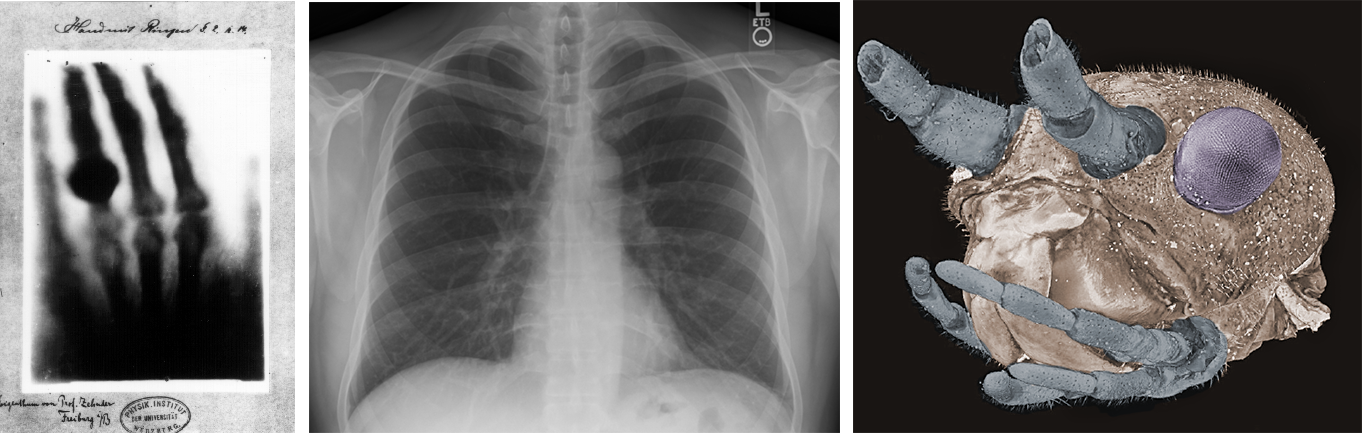
\includegraphics[scale=0.325]{figures/xrays_examples_all.png}}%
    \mbox{\includegraphicslabeledw[scale=0.32]{figures/xrays_hand.png}{a}}
    \mbox{\includegraphicslabeledw[scale=0.288]{figures/xrays_chest.png}{b}}
    \mbox{\includegraphicslabeledw[scale=0.368]{figures/xrays_insect2.png}{c}}
  }
  \caption[]{Evolution of X-ray imaging techniques. \textbf{(a)} First medical X-ray by Wilhelm R\"ontgen of his wife's hand. Image: Wikipedia, public domain. \textbf{(b)} X-ray radiography of a chest. Image: Wikipedia, public domain   \textbf{(c)} Volume rendering of the head of the stick insect \textit{Peruphasma schultei} imaged by a high resolution microtomography  \cite{vandeKamp13}.}
  \label{fig:xray_examples}
\end{figure*}

New methods and imaging techniques emerged with the development of \textit{synchrotron radiation}
sources. This radiation is generated using charged particle
accelerators.  Synchrotron radiation is emitted by the charged particles which are accelerated by magnetic fields on a circular trajectory in a storage ring. 

Modern 3rd-generation synchrotron radiation sources, equipped with high-resolution detector systems provide small beam size, high radiation intensity and high spatial resolution.
With the introduction of various X-ray optics the beam quality can be controlled, providing polychromatic or monochromatic radiation.
Synchrotron sources are expensive, not portable and usually are operated by large-scale facilities, which could limit a broad use of this technology. However, the unique quality of its probe make them a powerful tool for a wide range of X-ray experiments and applications.


\subsubsection*{X-ray Imaging Principles}
\label{xray_imaging_prnciples}

X-rays interact with matter either by \textit{photoelectric absorption} or \textit{scattering} (Compton and Rayleigh).  An absorption effect occurs when the X-ray photon is absorbed  in the course of liberating an electron from the inner shells of an atom. This contributes to the radiation dose defined as the amount of absorbed energy per unit of mass. This aspect is crucial for imaging of biological specimens. For a Compton scattering only a part of the X-ray photon  energy is used to free an electron  from an outer shell and the photon itself changes its direction, i.e. scatters \cite{Dougherty09}.
 
As a result of these interactions the intensity of the incoming beam is reduced. Various tissues or materials affect the changes in radiation intensity differently. In a homogeneous object this depends on its thickness $l$ along the direction of propagation and the attenuation coefficient $\mu$ of the material. The intensity $I$ of the incident X-ray beam after propagation through the sample of thickness $l$ is related to its initial intensity $I_0$ by the following expression:
$$I = I_0 e^{- \mu l},$$
which is known as a Beer - Lambert law.
    

%\change{From: Dougerty.
%Photoelectric absorption depends on the effective atomic number of the material, Zeff,
%and the x-ray energy, E, roughly as Zeff
%3/E3; and Compton scattering depends on the
%electron density of the material, ρelect, which varies roughly as Zeff, and the x-ray energy,
%as ρelect/E. Thus materials such as bone have a higher value of attenuation coefficient
%and attenuate x-rays more than soft tissues, as a consequence of their larger Zeff, and
%(photoelectric) absorption is the dominant interaction. Materials with a high effective
%atomic number, such as iodine (Zeff = 53) or barium (Zeff = 56), can be used to increase
%attenuation. They can be injected or swallowed to change the attenuation of soft tissues
%filled with the material compared to other soft tissues, and are known as contrast agents.
%For higher-energy x-rays, the overall attenuation is smaller with very much smaller
%photoelectric absorption and Compton scattering becoming dominant.}

Depending on the main effect of X-ray interaction with matter it is possible to classify  imaging techniques into \textit{absorption imaging} and \textit{phase-sensitive imaging}.
For the absorption imaging the contrast is produced by the attenuation of x-rays and is described as an amplitude modulation of the wave-field. In the case of  phase-sensitive imaging, contrast is governed by the
phase modulations due to the differences in spatial distribution of the refractive index.    
A number of phase sensitive imaging techniques might be used. A simple and popular method exploits the effect of propagation of the X-ray wave-field after its  interaction with the sample. Due to interference effects caused by the propagation,  the phase modulation can be reconstructed and visualized. For this technique a quantitative retrieval of the phase modulations is possible \cite{Cloetens99ab}, which allows to extract the real part of the refractive index in the interior of the investigated sample. 


%\subsubsection*{X-ray Sources Properties}
%X-ray source: flux, brilliance, coherence
%
%\change{From: Lukas. Important characteristic parameters of synchrotron sources are the source size and the
%brilliance [Rao93]. If the average electron velocity is defned parallel to y the brilliance
%is dened as (brightness/) where x and z are a measure of the source size in the
%x and z directions, respectively (i.e. FWHM of the spatial intensity distribution). The
%brightness is dened as the number of photons emitted per unit time into a unit solid
%angle and in a spectral bandwith = 10. }
%
%\change{From: Lukas. In the context of imaging applications, the low divergence of SR (especially of wigglers
%and undulators) allows one to place the object at a large distance from the source
%without losing a large portion of the emitted power. This is especially important for
%phase-contrast imaging (see Sect. 2.5.6): the high source-to-sample distances (and low
%source sizes compared to earlier generation synchrotron sources) enhance beam coherence
%signicantly. }


\subsubsection*{Beam Geometry}
Depending on the instrumental implementation of a X-ray source a number of different beam geometries are possible:

\begin{itemize}
\item \textit{Pencil beam}. The first X-ray source was implemented using a so-called pencil beam. For this geometry the cone of generated X-ray beams is filtered by a pinhole and, thus a point-like X-ray source is produced. A single detector is placed to the opposite side of the source to detect the X-rays.

\item \textit{Fan beam}. In this case the beam geometry is represented by a flat fan shape (divergent beam) and a detector system consists of an array of detector elements. Typically, the angle of beam divergence is small, as well as the size of the detection array.

\item \textit{Cone beam}. In this geometry the beam is a 3D cone with a wide angle of divergence and a large 2D detector is used. This technique is widely used in a laboratory-based X-ray setups. For this type of geometry the distance between the sample and the source is important, since it influences the object magnification in the detector plane.
Additionally, for image reconstruction algorithms the angular distribution of the incoming rays with respect to the rotation axis has to be taken into account \cite{Kak01}.

\item \textit{Parallel beam}.  The X-rays are coming parallel to each other and impinge on the sample perpendicular to its rotation axis. The 3D image reconstruction procedure for this type of geometry is the simplest and can be realized in an efficient way \cite{Kak01}.
\end{itemize}

%\begin{figure*}[t]
%  \centerline{
%    \mbox{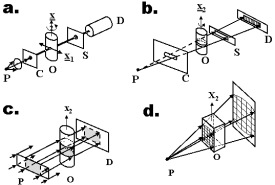
\includegraphics[scale=0.75]{figures/beam_geometry.png}}
%  }
%  \caption[]{Fast radiography of a feeding cockroach \textit{Periplaneta americana}. \textbf{Left:} Fist frame of the  radiographic sequence. (The background is removed and contrast is adjusted). \textbf{Right:} Computed motion field.  Color shows particular movement direction.}
%  \label{fig:beam_geometry}
%\end{figure*}

 
 In the current work all experimental results presented in the application sections are obtained using the parallel beam geometry. The most important aspect related to data analysis is the quality of 3D reconstructed images. Each beam geometry is associated with its own set of reconstruction artifacts \cite{Buzug08}. Therefore, the beam geometry, experimental parameters and the reconstruction algorithm strongly influence the later stages of data processing and analysis. We discuss these aspects in the Section \ref{computed_tomography} devoted to tomographic reconstruction.    




\subsubsection*{Detector System}

After the interaction with an object and propagation to the detector plane, X-rays are registered by a detector system. Two distinct classes of detectors are used in synchrotron radiation imaging \cite{Gruner01}:
\begin{itemize}
  \item \textit{Direct photon detectors}.  For this type of detector systems X-ray photons are converted directly into an electric charge. 
  \item \textit{Indirect detectors}. For the indirect detection system the incident photons first strike a material layer, called scintillator, which converts X-ray photons into visible-light photons. These photons are then detected by a visible-light detector.  
\end{itemize}

For each detector system a number of technologies are available, such as charge-coupled devices (CCD) and complementary metal-oxide-semiconductor (CMOS) cameras.
A substantial advantage of the indirect detector system is that a wide range of commercially available high-performance, visible-light cameras is available. With the recent developments such cameras can achieve a very high spatial resolution (down to 1.0 $\mu m$) and ultra fast data acquisition rates (up to 100.000 frames per second) \cite{Rack10}.    


\subsubsection*{Digital Image}
\label{digital_image}

\textit{Spatial resolution} is the capability of an image to represent object details. It can be characterized as the minimum separation distance of nearby features of the object which can still be recognized on the image as different structures.  In general, the spatial resolution of a digital image depends on the resolution of the imaging system described by its point spread function (PSF) and the pixel size of the detector system \cite{Dougherty09}.
The \textit{pixel size} of the digital detector is determined by the sampling frequency used to digitize the image signal and by the physical size and separation of the array elements within a 2D detector. Increasing the pixel size reduces the effective resolution, but can lead to the increased signal sensitivity.
The \textit{point spread function} describes the response of the imaging system given a point source or a point object. The width of the PSF function determines the size of the smallest detail that can be resolved. According to the sampling theorem \cite{Nyquist28}, the pixel size should be less or equal half the width of the point spread function in order to correctly sample an analog signal. For smaller pixel sizes the PSF spreads to several pixel locations and the resolution is reduced.

%\change{From: Lukas. The detective quantum e±ciency of a detector system is de¯ned by the signal-to-noise
%ratios (SNR) at the input and the output according to: (FORMULA) where at the input for photons with Poisson statistics (FORMULA)
%can be assumed. For an ideal detector the DQE equals 1 whereas real detectors show
%a DQE smaller than 1. Therefore the latter require increasingly better input statistics
%(e.g. by increase of the exposure time) the worse their DQE is.}



Another important characteristics of the digital image is the \textit{brightness resolution}. In a digital image differences between structures are represented by variations in brightness values. In X-ray imaging, these variations are determined by or related to the physical properties of a sample, such as sample thickness, material density and chemical composition. The aim of an imaging process is to distinguish between various parts of the sample, which differ in their structure or material composition. Ideally, this should also be valid if both materials differ from each other only slightly. To achieve this a detector system with a good brightness resolution should be used. This property is also called the \textit{dynamic range} of the detector system. The range of brightness variations which is recorded depends also on the number of bits used for quantization procedure (converting the analog signal to digital).  Most modern camera systems allow to record images in 12, 16 or 32-bit value formats. We discuss further aspects related to the brightness resolution in the Section \ref{contrast_adjustment}, which is dedicated to preprocessing of low-contrast image data.

\subsection{Experimental Methods}

In this section we briefly describe two imaging techniques, which will be employed in this work to acquire a sequence of time-lapsed X-ray images - radiography and tomography. For both experimental techniques we describe the advantages and shortcomings of its application with respect to its ability to capture spatio-temporal information. Moreover, we introduce typical challenges that arise during data processing and optical flow computation.

\subsubsection{Radiography}

\textit{Radiography} is a simple, yet powerful technique to visualize internal structures of a sample. For this purpose a sample is placed in the beam and properly aligned using manipulation devices (e.g. translation stages), so the optimal position in the field of view is achieved. As soon as the process of interest is triggered, a high speed camera records time-lapse projection images, called "radiograms". Many instrumental modifications for the radiography experiment setup are possible. They include the choice of the X-ray beam properties, positioning devices, source-to-sample and sample-to-detector distances, detector optics and the choice of digital camera or sensor.

We now describe a number of characteristic properties associated with the radiography technique.
Among the advantages of this method are:
 \begin{itemize}
  \item   High spatio-temporal resolution: Spatial resolution down to the micrometer scale and temporal resolution down to the microsecond range are achievable with modern detector systems \cite{Rack10}.
  %\item   Temporal resolution depends on the motion of the sample and the frame rate of a detector system. Assuming that the sample movement cannot be controlled, in order to improve temporal resolution, the acquisition frame rate should be increased. Having only one parameters to adjust, makes it is easier to perform an \textit{in-situ} or \textit{in-vivo} experiment.
  \item In most cases no complicated alignment of the sample is needed  - the sample is simply placed in the field of view of the detector system.
  \item Since the sample stage does not move during the data acquisition, the usage of complex or bulk sample environments is possible (e.g. furnace, high-pressure chamber, etc).
\end{itemize}
However, there are also a number of major drawbacks, that limit applicability of the radiography:
 \begin{itemize}
    \item   The main drawback of the radiography technique originates from the projection of 3D structures on a single 2D image plane. As a result, any depth information about internal 3D structures is inevitably lost.
    \item   For data processing methods, including correspondence problems (e.g. optical flow, object recognition), the superposition of 3D structures into a 2D plane imposes a critical challenge - the underlying assumptions on data constancy and the affine transformation model are no longer valid. For example, the change in orientation of the object in 3D space causes a redistribution of the projected thickness on the image plane. Thus, no reasonable assumption about the image data can be enforced. In some situations the movement in 3D space does not cause a change in the distribution of grey values in the projected 2D image. One example is  an object, which undergoes a translational movement perpendicular to the projected plane and the parallel beam geometry is used.         
 \end{itemize}


\begin{figure*}[ht]
  \centerline{
    \mbox{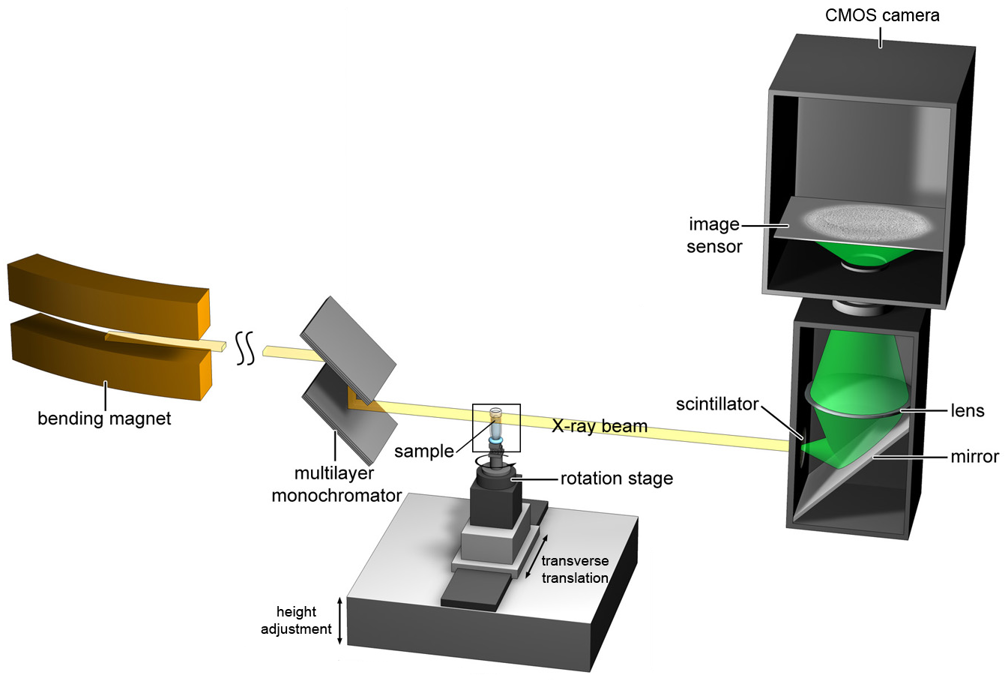
\includegraphics[scale= 0.30]{figures/tomo_setup.png}}
  }
  \caption{Experimental setup for propagation-based phase-contrast X-ray
microtomography. A photon beam is generated by the synchrotron. After the beam is shaped and filtered by the monochromator, the X-rays propagate over a large distance
to interact with the sample mounted on a rotation stage for
tomographic data acquisition. The 2D detector system consists of a scintillator, which converts X-rays into a visible light, a mirror, a lens and a CMOS digital camera. Image: \cite{Nature13} }
  \label{fig:tomo_setup}
\end{figure*}



\subsubsection{Computed Tomography}
\label{computed_tomography}

The previously described radiographic technique suffers from a major drawback - it only produces a projection of three-dimensional objects on the 2D detector plane. As a result the structures are superimposed with each other, which complicates their identification and analysis. Computed Tomography (CT) is a technique which has been developed to overcome this limitation. It provides a three-dimensional information about the inner structures of an object.
This technique consists of two stages. First, a series of radiographic projections from different directions are taken.
Then, a dedicated  algorithm is used to reconstruct a 3D volumetric image. 
The task for tomographic reconstruction is to perform the retrieval of the unknown object function from a series of its Radon transformations taken from different angles \cite{Kak01}.
There are two distinct classes of tomographic reconstructions:
\begin{itemize}
\item \textit{Analytical methods} are based on reconstruction steps using the Fourier transformation \cite{Kak01}. It is important to note, that such methods yield an exact solution of the inverse problem if a number of requirements are fulfilled. For large tomographic datasets these methods a preferred since they are typically less computationally demanding. Moreover, they are also less sensitive to noise and small data artifacts, thus producing more accurate results. One popular choice for such type of techniques is the \textit{filtered back-projection} (FBP) \cite{Kak01}.

\item \textit{Algebraic methods} represent an object as an array of unknown coefficients and model a ray transmission through the object as a mathematical function of these coefficients. Then a system of algebraic equations is solved to estimate the object. Usually this class of reconstruction methods is used if the requirements for the analytical methods are not satisfied. For instance, if the number of angular projections is insufficient. Or if the beam geometry and tomographic acquisition is hard to be modeled analytically, e.g. for diffraction tomography.         
\end{itemize}


A typical tomography setup is shown in Figure \ref{fig:tomo_setup}. Here we list advantages and drawbacks of the computed tomography technique.  Among the advantages are:
 \begin{itemize}
  \item   Computed tomography provides a 3D structural information about a sample. 
  \item   For the computation of optical flow having a 3D representation of a  scene and its objects means that there are no occlusions between different structures (as it happens for 2D images). This highly influence the accuracy of motion estimation and leads to better results.
\end{itemize}
Nevertheless, there are also a number of limitations:
 \begin{itemize}
  \item   The need of tomographic acquisition, which involves imaging of an object from multiple directions, can limit temporal resolution. This is especially critical for imaging rapid dynamical processes. 
  \item   The rotation of the sample on the tomographic stage could also restrain the use of sample environments (wiring, bulky instrumentation, etc), which cannot be rotated freely around an axis. 
  \item   To obtain tomographic volumes of a high quality, a large number of radiographic projections is required. Depending on the sample and properties of the X-ray radiation, it may result in a high dose deposition. This aspect is crucial for imaging living specimens and can limit the applicability of X-ray computed tomography.   
  \item Depending on the number of projections, image quality and specific image artifacts could appear and degrade the resulting 3D data. Compared to such image characteristics, such as noise and low contrast, these artifacts are difficult to correct. The presence of reconstruction artifacts significantly reduces the performance of optical flow methods. 
\end{itemize}



%\subsubsection{[OPTIONAL] Laminography}
%
%\begin{itemize}
%	\item   Method
%  \item   Setup. Setup scheme
%  \item   Advantages and shortcomings: Similar to CT. What else?
%  \item Short experiment example (Inspection Flip-chip devices)
%	\item References
%\end{itemize}



%--------------------------------------------------------
\section{Variational Optical Flow}
%--------------------------------------------------------

\textit{Optical flow} is one of the major problems in \textit{Computer Vision}.  Given a sequence of images the aim is to determine the correspondences between them. A method to find the displacement field which maps all image points from the first frame to their new locations within the second frame is called \textit{optical flow}. Following a formulation from the seminal work of Horn and Schunck \cite{HornSchunck81}, the motion field is the 2D projection of the actual 3D motion of objects and scene, where the \opticalflow is the \textit{apparent} motion of the brightness patterns depicted on the image.   In our work we extend the definition of optical flow as an actual 3D motion of internal structures when applied to 3D tomographic volumes.

\Opticalflow is useful for a variety of different applications such as robot vision, driver assistant systems, object tracking and stereo reconstruction, video analysis and processing \cite{Wolf96, Sudhir96, Kastrinaki03, Hu04}.    In this work we employ \opticalflow methods to perform data analysis and investigate of a wide range of applications related to the field of X-ray imaging. One example is given in Figure \ref{fig:example_feeding_insect}, where \opticalflow is used to capture real-time movements of the feeding cockroach.

\begin{figure*}[ht]
  \centerline{
    \mbox{\includegraphicslabeledb[scale=0.33]{figures/bug_full_original_enh.png}{a}}
    \mbox{\includegraphicslabeledb[scale=0.33]{figures/bug_full_colors.png}{b}}
    \mbox{\includegraphicslabeledb[scale=0.5]{figures/color_code_inverted.png}{c}}
  }
  \caption[]{Fast radiography of the feeding cockroach \textit{Periplaneta americana}. \textbf{(a)} First frame of the  radiographic sequence (the background is removed and contrast is adjusted). \textbf{(b)} Computed flow field, which captures the movements of the insect. \textbf{(c)}  Color coding: color represents direction and its brightness represents flow magnitude.}
  \label{fig:example_feeding_insect}
\end{figure*}


\subsection{Related Work}

The research on \opticalflow estimation advances is rapidly. The methods become more accurate, robust with respect to challenging data and flexible to model various scene and motion scenarios. In the scope of this work we restrict ourselves to a specific class of approaches used to determine the optical flow, so-called \textit{variational methods}. These methods are recognized as one of the most accurate and best understood techniques for the \opticalflow computation \cite{Middl, Sun14}. 

Recently a number of important contributions to the field of \opticalflow estimation were made. In the work of Bruhn \cite{BruhnThesis} a systematic taxonomy and quantitative evaluation of variational \opticalflow methods was presented. A common notation as well as an extensive list of available models allows to construct an optical flow framework, suitable for a wide range of applications. 
Development of a novel database for the evaluation of optical flow techniques has led to rapid improvements and understanding of optical flow methods \cite{Middl} . 
A vast amount of literature on motion estimation techniques propose sophisticated models and multiple features. This  makes it hard to evaluate the performance of the individual components. In Refs. \cite{Sun10, Sun14} the authors provide an overview over current state-of-the-art \opticalflow methods and reveal the "secrets" behind the most successful models.
Recently, some of the authors reported that even the most advanced approaches yield poor results on a challenging real-life data. This highlights the importance of work on  robust optical flow methods designed for a particular task or application. A number of application specific optical flow evaluation databases has already emerged \cite{Adato07, Geiger12}.

Many of the today's state-of-the-art variational \opticalflow methods still resemble the original
formulation by Horn and Schunck \cite{HornSchunck81}. This model combines a \textit{data term} that imposes constraints on image features which should be matched and a \textit{smoothness term} which regulates the properties of the flow field. A global energy functional containing both constraints is then minimized to find the solution. In this section we describe important work related to the modeling of data and smoothness assumptions, as well as the optimization procedure.  We also give a short outlook of works where optical flow methods has been applied.

There are many approaches and interesting concepts which go beyond the scope of this work. For example, we exclude the discussion of photometric data terms constancy assumption based on color information \cite{Mileva07},  motion with transparency or layered models \cite{Jepson93, Wang93, Ju96},  incorporation of feature descriptors (i.e. SIFT) to refine motion estimation during coarse-to-fine strategy \cite{Xu10},  combination of optical flow estimation and image segmentation \cite{Black96b, Zitnick05, Xu08}, or the use of non-convex optimization strategies.  We will restrict ourselves only to those approaches which are suitable for the application on the X-ray image data and can be incorporated to the variational framework. 

\subsubsection{Data Assumptions}

In the literature, there are two major directions for the formulation of data constraints: design of robust data terms, which improve the performance on problematic image data and incorporation of additional information to model various aspects, such as illumination changes and different motion models. 
The first approach for the robust data term was proposed in the work of Black and Anandan \cite{Black91, Black96}, where the quadratic function of the original Horn and Schunck method was replaced by a non-quadratic variant. The robust modeling of data constraints become an important factor in the construction of accurate optical flow methods \cite{Brox04, Lempitsky08, Xu10, Middl, Sun14}. 
In order to handle varying illumination conditions,  higher order constancy assumptions \cite{Schnorr93, Schnorr94,  Brox04, Papenberg06, HarmonyFlow} or special image filtering are proposed \cite{Mileva07, Wedel09, HarmonyFlow}. To improve the performance of data constraints for noisy images some of the authors suggested a local-global data term \cite{Bruhn02, Bruhn05a}, which takes into account the information around a local region.  

\subsubsection{Regularization}

The regularization of flow fields involves two main aspects: discontinuity preserving motion estimation and incorporation of temporal information.
The first approach to use adaptive smoothness was proposed by Nagel et al. \cite{Nagel83, Nagel86}. This idea has been developed in a number of approaches which assume image-driven \cite{Schnorr93, Alvarez99} or flow-driven smoothness \cite{Shulman89, Schnorr94}.  In Ref. \cite{Sun08} the authors combined the advantages of both methods to obtain precise motion discontinuities and avoid oversegmentation problems. In their work the smoothness direction is adjusted to image edges and smoothing amount to the flow gradient. In Ref. \cite{HarmonyFlow} the authors generalized this idea to obtain a \textit{complementary smoothness} term.  Such approach regulates the smoothness direction according to the data constraint, instead of image edges.

The idea to assume the smoothness also in temporal direction was first investigated  by \cite{Murray87} and extended for continuous models in \cite{Nagel90}. A discontinuity-preserving spatio-temporal smoothness was proposed in \cite{Weickert2001b} and used for a number of highly accurate \opticalflow models \cite{Brox04, HarmonyFlow, Volz11}.

\subsubsection{Solution}

To find a solution of variational methods in the presence of large displacements it is common to use a coarse-to-fine strategy \cite{Black96, Memin98, Brox04, Xu10}. For the construction of image pyramids and in order to perform image warping a bicubic interpolation is commonly used \cite{Sun10}.
In order to represent image gradients a second order derivatives, as well as temporal averaging are among good practices \cite{Wedel09, Sun14, HarmonyFlow}. A number of efficient computation models were proposed, such as multigrid methods \cite{Bruhn05, Bruhn06b}. Furthermore, a popular trend is a fast implementation of variational methods using graphical processing units (GPU) \cite{Wedel09, Gwosdek12, Bao14}.


\subsubsection{Applications}


Optical flow methods are widely used in the native field of Computer Vision, for such applications as video surveillance and analysis \cite{Kastrinaki03, Hu04}, video compression \cite{Wolf96} and video annotation \cite{Sudhir96}. Recently, the usage of optical flow methods become important for data analysis in the fields of biological imaging and life sciences, as well as in other research fields. Examples include: zebrafish development \cite{Amat13}, monitoring of plant growth \cite{Barron97}, in-vivo blood flow measurements \cite{Vennemann07}, modeling and correction of respiratory motion \cite{McClelland13} and analysis of cardiac images \cite{Xu10b}.


Various parts of the current work were presented in publications, dedicated to  X-ray imaging \cite{Baumbach09, Rack10, Altapova12}, applied for \textit{in-situ} studies of advanced materials \cite{Zabler10, Myagotin12, Zabler13} and for \textit{in-vivo} investigation of various biological questions \cite{Betz08, Nature13, van13, Moosmann14, dosSantosRolo14}. 


\subsection{General Model}
\label{general_model}

A general model for variational methods was proposed by Horn and Schunck in 1981 \cite{HornSchunck81}. This technique determines the unknown displacement field as a minimal solution of the  \textit{energy functional}. In general, such energy-based formulations are composed of two parts: a data term which assumes constancy of specific image features, and a smoothness term which regularizes the spatial variation of the flow field.
 
The classical \opticalflow approach of Horn and Schunck consists of a \textit{brightness constancy} assumption and a \textit{homogeneous} smoothness term. The first constraint states that after the displacement the  brightness value remains constant and the second constraint assumes that the motion field varies smoothly in all directions.

In order to formulate the \opticalflow model we consider a time-lapse sequence of images $I(x,y,t)$, where $(x,y)$ are the pixel coordinates within an image domain $ \Omega_{2} \subset     \mathbf{R}^2$ and $t$ denotes time frame. Then, the brightness constancy assumption can be expressed by:
\begin{equation}
	I(x+u(x,y), y+v(x,y), t+1) = I(x,y,t),
	\label{eq:brightness}		
\end{equation}
where ($u(x,y),v(x,y)$) is the displacement field from frame $t$ to $t+1$. To simplify the formulation of model assumptions, we will use the short notation $u, v$ for the displacement field components  instead of $u(x,y),v(x,y)$.
Assuming that the displacement components are small and changing continuously, we can approximate the non-linear equation (\ref{eq:brightness})  using a first order Taylor expansion. We obtain the so-called \textit{ linearized optical flow constraint}:
\begin{equation}
	I_{x}u + I_{y}v +I_{t} = 0.
\end{equation}

The \opticalflow cannot be  uniquely computed at a single point since the displacement is given by two components, while the change in image brightness provides only one constraint. In the literature this is known as the \textit{aperture problem} \cite{Bertero88}. There are two different cases of this issue. If only one component of the image gradient can be computed, it is possible to determine the flow component parallel to the direction of image gradient, so-called \textit{normal flow}.
In the second case, in homogeneous image regions the brightness gradient vanishes completely, so no appropriate correspondence can be found. 

To overcome this problem, the method proposed by Horn and Schunck introduces an additional constraint which assumes the spatial smoothness of the flow field. Such constraint can be expressed by penalizing the spatial flow gradients, given by $\nabla_{2}u$ and $\nabla_{2}v$.
Both, the brightness constraint and the smoothness constraint can be integrated in the energy functional to obtain the classical Horn and Schunck method:

\begin{equation}
E_{\text{HS}}(u,v) = \int_{\Omega_{2}}{(I_{x}u + I_{y}v +I_{t})^2 + \alpha (|\nabla_{2}u|^2 + |\nabla_{2}v|^2) \text{d}x \text{d}y},
\end{equation}
where $|f| = \sqrt{f^2_x + f^2_y}$ is the magnitude and $\nabla_2 = (\partial_{x}, \partial_{y})$ denotes the spatial gradient. The parameter $\alpha$ is called \textit{regularization} or \textit{smoothness parameter} and controls the amount of required smoothness of the resulting flow field. 

The variational \opticalflow methods based on the Horn and Schunck model can be written in a more general form:

%$$E(u,v) = \int_{\Omega_{2}}{D(I,u,v) + \alpha \: S(I,u,v) dx dy},$$
$$E_{\text{general}} = \int_{\Omega_2}{(D(I, u,v) + \alpha  \: S(I, u,v)) \: \text{d}x \text{d}y},$$
where $D(I,u,v)$ imposes constraints on image features which should be matched and $S(I, u,v)$ regulates the smoothness properties of the flow field. Both parts of this general \opticalflow framework can be customized and adapted for the specific data properties and motion models. In Chapter \ref{optical_flow_methods} we present different approaches to construct accurate and robust variational \opticalflow models and discuss how these techniques could be applied for the particular task of X-ray data analysis.

In order to find the solution of the \opticalflow problem we are interested to have energy functionals which are \textit{convex}. For such functionals a \textit{unique solution} exists and it can be found using \textit{globally convergent} algorithms. In contrast, for non-convex approaches \textit{multiple local minima} can be present and optimization algorithms may suffer from getting trapped in local minima, thus providing inaccurate results. For the Horn and Schunck method linearization of the brightness constraint must be performed in order to obtain a convex functional. Such linearization step does not affect the accuracy of the result as long as only small displacements for the scene are considered. In order to cope with large displacements linearization procedure cannot be applied and the original non-linear variant of the data term must be used. In Section \ref{large_displacements} we will introduce a \textit{coarse-to-fine strategy} based on the theory of warping which allows to solve non-convex energy functionals for our problem.


 
%--------------------------------------------------------
\section{Aims of the Work}
%--------------------------------------------------------

As it was discussed in the introductory section, time-resolved X-ray imaging methods provide a wide range of possibilities for the research of dynamical processes. 
It is a challenging task, however, and involves many steps to get from the initial idea of the experiment to the final scientific result. 
After an experimental setup is prepared and carefully adjusted, the original raw data is recorded by a detector system.  The acquired data have to be inspected and evaluated to ensure that the desired image quality is achieved and the events of interest are captured.
At this step important adjustments could be introduced to improve the results. The raw experimental data coming from the detector system is usually not suited for the immediate analysis, since images often contain artifacts.  Thus, an artifact correction and data enhancement procedure is desirable. The quality of time-resolved X-ray data is immensely diverse. Data related properties, such as image resolution, signal-to-noise ratio, features contrast and underlying motion model, influence the performance of data processing routines. To automatically capture the dynamics of a process an appropriate computation algorithm should be employed.  In this work we use \textit{variational optical flow} as the core method to extract temporal information. 
%An overview of a typical experiment workflow is presented in Figure \ref{fig:pipeline_scheme}.   
%\begin{figure*}[ht]
%  \centerline{
%    \mbox{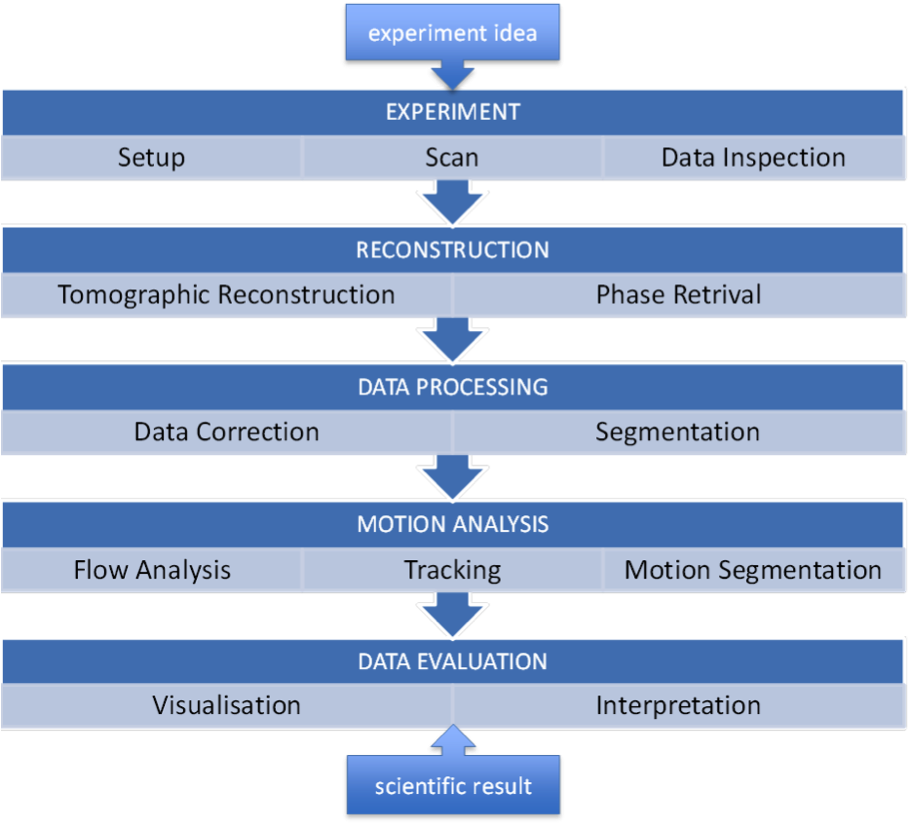
\includegraphics[scale=0.75]{figures/pipeline_scheme.png}}
%  }
%  \caption[]{\todo{Change} A general workflow for  time-resolved X-ray data analysis.}
%  \label{fig:pipeline_scheme}
%\end{figure*}
      
The main goal of our work is to cover, investigate and implement all the aspects that are important for automated analysis of time-resolved X-ray data. To achieve this we proceed with the following steps:
        
\begin{itemize}
    \item provide a detailed classification of X-ray data, including the description of image quality, motion types and features of interest. This taxonomy should serve as a reference point for the development of image preprocessing, data analysis and motion estimation procedures
    
	\item develop image preprocessing methods to enhance the original (raw) X-ray data
	
	\item perform systematic evaluation of state-of-the-art \opticalflow techniques, make quantitative analysis of their components and choose the most robust and accurate approaches
	
	\item introduce a flexible framework based on variational \opticalflow methods to extract dynamical information from time-lapsed datasets
	
	\item provide automated confidence measures to ensure the reliability of motion estimation. Such measures should also assist with the automated optimization of model parameters
	
	\item develop an extensive data analysis toolkit including automated tracking, flow analysis, motion-based segmentation, image registration and detection of temporal changes
	
	\item implement the developed techniques for 4D data (3D + time) to enable analysis of tomographic data
	
	\item provide an efficient implementation of optical flow methods using advanced numerical schemes and computations on graphics processing units (GPUs). Thereby, the processing of a vast amount X-ray data - long image sequences and large tomographic volumes - becomes feasible 
	
	\item apply the devised optical flow and data analysis techniques to investigate a number of scientific problems from various research fields 
\end{itemize}

All the aforementioned topics are essential for the subject of this thesis, therefore we consider them as a complete framework. However, some parts of this work are also useful as isolated topics.  As an example - in Section \ref{data_taxonomy} we provide an approach for qualitative data taxonomy and in Section \ref{data_preprocessing}  we present image processing routines to enhance the original X-ray data. These steps are general for various data analysis problems that are not related to analysis of dynamics (e.g. image segmentation). The variational \opticalflow methods which we use in this work could be substituted by any other technique solving the same class of problems, i.e. finding correspondences between time-lapse images. Therefore, the information presented in other parts, such as in the chapters dedicated to data analysis or applications are still valuable. The current work is interdisciplinary and closely related to the fields of Computer Science, X-ray imaging, Material and Life Sciences.

 






%******************************************************************
%******************************************************************
\chapter {Optical Flow Methods}
\label{optical_flow_methods}
%******************************************************************
%******************************************************************

This chapter is dedicated to a detailed description of \opticalflow methods. First we introduce quality measures for motion estimation. Using these measures it is possible to assess the accuracy of the result of the optical flow estimation if the ground truth is known. Then, we present different approaches for the construction of variational models and discuss how these techniques could be applied for X-ray data. This part is divided into several sections, which are devoted to (i) the construction of data constancy assumptions, (ii) robust data terms and (iii) smoothness assumptions. Afterwards we introduce of automated confidence measures.
Next, we extend the devised 2D optical flow models to 3D, which enables us to perform data analysis of tomographic data.  Afterwards, we explain how a variational functional is solved numerically using iterative methods. Furthermore, we discuss various computational aspects such as derivatives discretization and implementation of multi-level computation.


%--------------------------------------------------------
\section{Modeling}
%--------------------------------------------------------

\subsection{Quality Measures}
\label{quality_measures}

Before we start with the description of \opticalflow methods, we first present quality measures which allow for quantitative comparison of different approaches if the ground truth  for \opticalflow is known. We will employ these measures in our extensive performance studies of optical flow methods and data processing techniques in the section \ref{experiments_synthetic_data}. It is important to note, that the performance of an algorithm cannot be described by a single measure. Instead, to show the performance with respect to different characteristics of an image we employ a set of measures. However, we do not show all the available measures for every evaluation. Instead, we use only those measures which are of interest for the particular evaluation case.



\subsubsection{Angular Error}
\label{angular_error}

In the recent years the most widely used performance measure for \opticalflow was the \textit{angular error} (AE). It is given by an angle between a computed flow vector $ \textbf{w} = (u, v)$ and a ground truth flow $\textbf{w}_{GT} = (u_{GT}, v_{GT})$, which can be computed as a dot product of both vectors, divided by the product of their length: 
$$ AE = \text{arccos} \Bigl (\frac{u \cdot u_{GT} + v \cdot v_{GT} + 1.0} {\sqrt{u^2 + v^2 + 1.0} \sqrt{u_{GT}^2 + v_{GT}^2 + 1.0}   } \Bigr ). $$

Note, that angular error contains an additional scaling constant (1.0) to convert from
pixels coordinates to the angular space. This measure was introduced in Ref. \cite{Fleet90} and was used in one of the first surveys on the performance of \opticalflow methods by \cite{Barron94}. The main purpose of the \textit{AE} is to provide a relative performance measure that could be used for all flow scales and is not causing problems for zero motion. However, it is important to note that errors in regions with fast motion are penalized less than errors in slow regions, which is a result of length normalization for this measure. Despite the fact, that the angular error was widely used in the previous work on \opticalflow methods its properties are not desirable for a robust and unbiased measure.


\subsubsection{Endpoint Error}
\label{endpoint_error}

Another measure to estimate the performance of flow field computation is the \textit{endpoint error} (EE) \cite{Otte94}. This measure captures the absolute difference between two flow vectors $\textbf{w} = (u, v)$ and $\textbf{w}_{GT} = (u_{GT}, v_{GT})$:
$$ EE = \sqrt{(u_{GT} - u)^2 + (v_{GT} - v)^2}. $$
The endpoint error does not suffer from the drawbacks of angular error measure: it can be applied for the whole range of flow scales and all of them contribute equally. It is also a much more appropriate way to evaluate the differences between vectors if not only the direction, but also the difference in magnitude of the flow is important. Currently this measure is prevalent in the literature \cite{Sun10, Middl} and will also be used to evaluate the performance of \opticalflow methods in this work. 


\subsubsection{Error Statistics}
\label{error_statistics}

In order to evaluate the result of an \opticalflow computation for a given image sequence one is interested in a quantitative description of the quality of the output. A straightforward statistical measures are the average error  and the standard deviation \cite{Barron94}. Despite the fact, that both measures can be used to evaluate the overall performance, they are not optimal for measuring the performance on challenging image data or more complex scenes (e.g. a scene for which the background with little or no motion is prevalent).

Following the ideas presented in Ref. \cite{Middl} we compute robustness measures \cite{Scharstein02}. For simplicity we also keep their notation for the presented statistical measures and denote by \textit{RX} the percentage of pixels that have an error measure larger then \textit{X}. In particular, we compute \textit{R0.5}, \textit{R1.0}, and \textit{R2.0} for the endpoint error. 

%In addition, we compute robust accuracy measure \cite{Seitz06} for which \textit{AX} denotes the accuracy of the error measure at the X-percentile, after sorting the errors. We report the statistics for \textit{A50}, \textit{A75}, and \textit{A95}.

\subsubsection{Statistics Regions}
\label{statistics_regions}

The reliability of \opticalflow methods differs in various image regions. In particular, it is difficult to compute the flow around motion discontinuities, inside noisy regions, near artifacts or in homogeneous regions. Thus, it is reasonable to distinguish between such regions and evaluate their statistics separately. This can provide insights how different \opticalflow models perform for in a particular situation.  In the common benchmark for \opticalflow methods \cite{Middl} three types of regions were evaluated: all image data (\textit{All}), around motion discontinuities (\textit{Disc}), and in textureless regions (\textit{Untext}). In \cite{Middl} it is concluded that \textit{Disc} regions contain the most challenging data for the computation of optical flow. In contrast, 
textureless regions are not hard to recover, as soon as global optimization techniques (employing smoothness constraints) are used.
In the Section \ref{modeling_xray_data} to evaluate the performance of \opticalflow models on corrupted data we intentionally introduce synthetic artifacts. In this case we are interested to measure error statistics inside these regions and in a local neighborhood around them. We denote such regions with data outliers as \textit{Err} regions.

To compute a mask for the \textit{Disc} regions we take the gradient of
the ground truth displacement field, compute its magnitude, apply a threshold for the magnitude, and then dilate the resulting mask with a $9 \times 9$ stencil. \textit{Untext} regions are computed in a similar manner, but using a $3 \times 3$ stencil size \cite{Middl}. 


%\todo{Consider object and background regions}.



%-------------------------------------
\subsection{Data Constancy Assumptions}
\label{data_constancy_assumptions}
%-------------------------------------


To solve a correspondence problem one has to assume constancy of certain image features. For the choice of an appropriate constancy assumption all prior knowledge about the acquisition method, imaging conditions and the underlying scene should be taken into account. The selection of suitable data  assumptions is essential and should be well adapted for the specific image data. In this section we provide an overview of data constancy assumptions. For each data assumption we discuss the aspects related to its usage on X-ray data.  Note, that in the current work we do not aim to provide a complete list of all data constraints available in the literature. We focus only on those approaches, which can be practically used for highly challenging  X-ray data. For example, we exclude the discussion of data terms based on color information.

\subsubsection{Image Smoothing}
\label{image_smoothing}

The computation of optical flow is usually preceded by a \textit{presmoothing} step. The aim of this step is to eliminate image noise. The most common procedure is to convolve the initial image $I_0$ with a \textit{Gaussian kernel} $K_{\sigma}$ with a standard deviation $\sigma$. High frequency variations are removed due to \textit{low-pass} filtering effect of Gaussian filter.
Furthermore, presmoothed image becomes infinite times differentiable, which is an important property to guarantee \textit{well-posedness} of the inverse problem \cite{HSSW01}. 
%------------------
% Not very useful
%------------------
%An example of the Gaussian filtering of X-ray radiographic image is presented in Figure \ref{fig:2_smooth}.

It is important to note that an appropriate choice of the smoothness degree is a crucial task. On the one hand, image presmoothing allows to improve image data and increase signal-to-noise ratio. On the other hand, oversmoothing destroys small image details and edges, which can lead to an inaccurate \opticalflow estimation. For the description of an optical flow model we always provide the initial smoothness level together with other model parameters.

%\begin{figure*}[ht]
%  \centerline{
%    \mbox{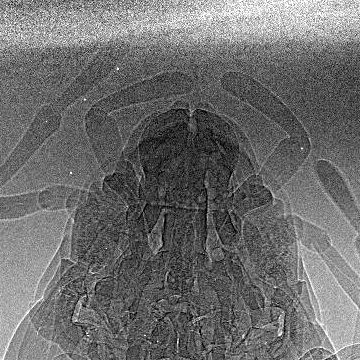
\includegraphics[scale=0.4]{figures/noisy_insect_0p0.png}}
%    \mbox{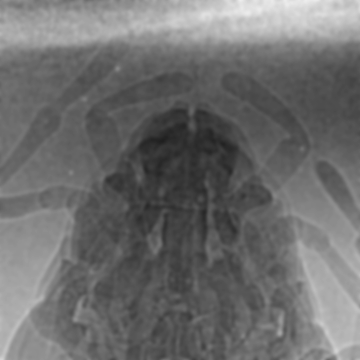
\includegraphics[scale=0.4]{figures/noisy_insect_2p0.png}}
%    \mbox{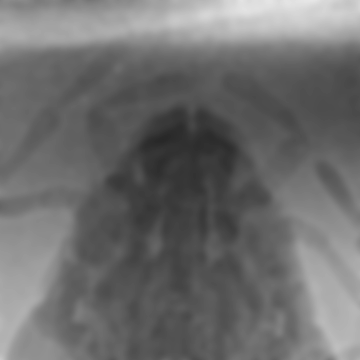
\includegraphics[scale=0.4]{figures/noisy_insect_4p0.png}}
%  }
%  \vspace{3pt}
%  
%  \caption[Performance of Gaussian smoothing]{Performance example of Gaussian smoothing on noisy images of feeding cockroach. Standard deviations $\sigma$ = 0, 2.0 and 4.0 respectively.}
%  \label{fig:2_smooth}
%\end{figure*}



\subsubsection{Brightness Constancy Assumption}
\label{brightness_constancy_assumption}

The simplest assumption is that moving objects within a scene do not change their appearance. In other words, the corresponding pixels have the same brightness values \cite{LucasKanade81, HornSchunck81}. This data constraint combines assumptions about the reflectance properties of the scene and illumination changes. For two subsequent image frames on time $t$ and $t+1$ the brightness constancy assumption can be expressed by:
\begin{equation}
I(x+u, y+v, t+1) = I(x,y,t).
\label{eq:constraint}	
\end{equation}
Under the assumption that the displacement components are small, this non-linear implicit equation for $(u,v)$ can be linearized by performing a first-order Taylor expansion. For a function $I(x+u, y+v, t+1)$ around the point $p = (x, y, t)$ the Taylor expansion is given by:
%------------------
% Not very useful
%------------------
%\begin{figure*}[!h]
%  \centerline{
%    \mbox{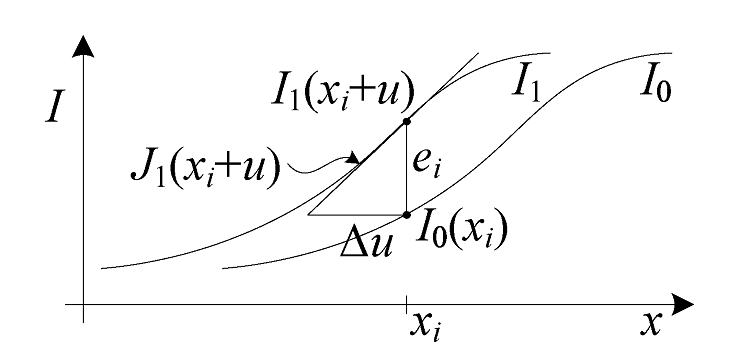
\includegraphics[scale=0.3]{figures/taylor.png}}
%  }
%  \caption[Taylor]{\todo{Correct image} Taylor series approximation of a function $I$ around a point $x_i$ and the incremental computation of the
%optical flow correction amount.}
%  \label{fig:taylor}
%\end{figure*}
$$I(x+u, y+v, t+1) \approx I(x,y,t) + I_{x}u + I_{y}v +I_{t}.$$
Using this approximation, the equation (\ref{eq:constraint}) can be rewritten as:
\begin{equation}
I_{x}u + I_{y}v +I_{t} = 0.
\label{eq:constraint2}	
\end{equation}
which is known in the literature as the \textit{linearized \opticalflow constraint}.

To shorten the formulation of \opticalflow constraints we follow the idea presented in \cite{Bruhn2006} and rewrite the equation (\ref{eq:constraint2}) in the following way:
$$ I_{x}u + I_{y}v +I_{t} = \nabla_{3}^{\top}I\textbf{w}   $$
where $ \textbf{w} = (u, v, 1)$ and $\nabla_{3} = (\partial_{x}, \partial_{y}, \partial_{t})$ denotes the image gradient.

Since both positive and negative deviations from the data constraint should be taken into account, in the work of  \cite{LucasKanade81, HornSchunck81} the authors incorporate its square to the final version of data term. The brightness constancy assumption in a short notation is given by:
$$ D_{grey}(I,\textbf{w}) = (\nabla_{3}^{\top}I\textbf{w})^2.$$



\subsubsection{Gradient Constancy Assumption}
\label{gradient}

The brightness constancy assumption can be used as long as illumination conditions and thus the corresponding pixel grey values between successive frames are not changing. If these assumptions are violated, data constraints that are invariant under brightness changes must be imposed.  To cope with such situations, spatial brightness derivatives are introduced \cite{Uras88, Schnorr93, Brox04, Papenberg06}, since they remain constant in the presence of \textit{additive} illumination.

Taking spatial derivatives of the image brightness for both spatial components we obtain two constraints given by:
$$ I_{x}(x+u, y+v, t+1) = I_{x}(x,y,t), $$
$$ I_{y}(x+u, y+v, t+1) = I_{y}(x,y,t). $$
After linearization step is performed, both constraints using a short notation are given by:
$$ \nabla_{3}^{\top}I_{x}\textbf{w} = 0, $$
$$ \nabla_{3}^{\top}I_{y}\textbf{w} = 0. $$
Combining both constraints gives us the required data term using gradient constancy assumption:
$$ D_{grad}(I,\textbf{w}) = (\nabla_{3}^{\top}I_{x}\textbf{w})^2 + (\nabla_{3}^{\top}I_{y}\textbf{w})^2. $$

It is important to note - that in contrast to the brightness assumption - the gradient assumption provides two independent constraints instead of one. This gives an additional information and could be used to overcome the aperture problem \cite{HornSchunck81}.
However, despite the advantages of gradient assumption in the presence of global brightness changes, this constancy assumption is much more sensitive to noise.
This property of a data constraint is crucial for noisy data, such as often encountered in time-resolved X-ray imaging.  We investigate the influence of noise on the performance of data constancy assumptions in the experimental section \ref{experiment_data_terms_for_noisy_data}.


\subsubsection{High-Order Constancy Assumptions}
\label{high_order_constancy}

The use of derivative-based constancy assumptions is not limited to the constancy of the brightness gradients. Higher-order derivatives, such as the Laplacian could also be employed for formulations of constancy assumptions. However, some of them are not suited for all types of motion. This is due to the fact, that some of these assumptions (e.g. brightness gradient) contain directional information, so they are dependent on the spatial orientation of image features. For an extended taxonomy of possible higher-order constancy assumptions the reader is referred to the literature \cite{Papenberg06}. Here we describe two constraints based on higher-order derivatives which can be potentially useful.
\\
\\
\textbf{Laplacian Constancy Assumption}
\\
As it was mentioned in the previous section, directional information contained in data constraints may introduce some difficulties in the presence of fast rotational motion. To overcome this problem one can restrict to direction-invariant features such as constancy of Laplacian \cite{Papenberg06}, which is given by:
$$ \Delta_{2} I(x+u, y+v, t+1) - \Delta_{2} I(x,y,t) = 0, $$
where $\Delta_{2} I = I_{xx} + I_{yy} $.
The linearized data term in a compact form reads:
$$ D_{lapl}(I,\textbf{w}) = ( \nabla_{3}^{\top}(\Delta_{2}I) \textbf{w})^2.$$

In general, all constraints based on higher-order derivatives are more sensitive to noise and data artifacts than their counterparts based on image intensity. This crucial property must be taken into account for modeling of a suitable energy functional. We compare the performance of the brightness constancy assumption and assumptions based on  derivatives in the evaluation section \ref{experiment_data_terms_for_noisy_data}.
\\
\\
\textbf{Gradient Norm Constancy Assumption}
\\
Another possibility to deal with  fast rotational motion is to use the magnitude of the gradient, instead of spatial gradients themselves (\cite{Papenberg06}).
The obtained data constraint and its corresponding data term are given by:
$$ |\nabla I(x+u, y+v, t+1)| - |\nabla I(x,y,t)| = 0 $$
$$ D_{grad-norm}(I,\textbf{w}) = (\nabla_{3}^{\top}|\nabla I| \textbf{w})^2, $$
where $|\textbf{f}| = \sqrt{f^2_x + f^2_y}$.

\subsubsection{Assumptions on Multiple Image Features}
\label{assumptions_on_multiple_image_features}

To improve the accuracy of \opticalflow computation it might be a good idea to combine assumptions on various image features. The model based on multiple constancy assumptions provides more flexibility and may lead to a significant improvement of the results. An example for this approach a linear combination of both brightness and gradient constancy assumptions \cite{Brox04, HarmonyFlow}. Its data term reads:
$$ D_{brigh+grad}(I,\textbf{w}) = \beta_{1}( \nabla_{3}^{\top}I \textbf{w})^2 + 
\beta_{2} ((\nabla_{3}^{\top}I_{x}\textbf{w})^2 + (\nabla_{3}^{\top}I_{y}\textbf{w})^2), $$
where $\beta_{1}$ and $\beta_{2}$ are parameters to control the contribution of the individual constancy assumption to the overall data term.

Multiple image assumptions might also be useful to incorporate the information obtained by different contrast mechanisms, for example absorption and phase contrast. An alternative approach to include multiple assumptions on image features (and more generally, on different optical flow models) was presented in \cite{Lempitsky08}. In this work a series of candidate flow fields is computed using different algorithms or model parameters. Then a final flow is determined by an additional optimization problem. This idea corresponds to a so-called \textit{fusion} approach. 


\subsubsection{Landmarks-driven approach}
\label{landmarks}


It is possible to incorporate user-defined landmarks to an \opticalflow model. This procedure is especially useful if the manual tracking of some objects or their parts is performed. Thus, it is possible to combine the  information specified by an user with an automated flow computation. As it was shown in \cite{Fischer03} it is not convenient to embed the information about landmarks into the original energy functional. It is much more straightforward to modify the corresponding Euler-Lagrange equations (see Section \ref{minimization_procedure}) directly. We illustrate this on the example of the Horn and Schunck model. 
For this purpose we introduce a confidence map $c_{GT}(x,y)$, which equals to 1 or 0, depending on whether for a pixel position $(x,y)$ the ground truth landmark is given.

Embedding the confidence map $c_{GT}(x,y)$ into the Euler-Lagrange equations (\ref{eq:euler}) we obtain:
$$ (1 - c_{GT}) (I^2_x u + I_x I_y v + I_x I_t - \alpha \: \textrm{div} (\Psi'(|\nabla u|^2 + |\nabla v|^2) \cdot \nabla u )) + c_{GT}(u - u_{GT}) = 0, $$
$$ (1 - c_{GT}) (I_y I_x u + I^2_y v + I_y I_t - \alpha \: \textrm{div} (\Psi'(|\nabla u|^2 + |\nabla v|^2) \cdot \nabla v )) + c_{GT}(v - v_{GT}) = 0. $$
If the ground truth displacement is not provided we obtain the original version of Euler-Lagrange equations.
For the other case the solution is set to the ground truth result $u = u_{GT}, v = v_{GT} $. After the flow field is modified according to information provided by landmarks it is propagated to the neighbouring pixels via the regularization term (see Section \ref{smoothness_assumptions}). Furthermore, to enhance the influence of the ground truth it makes sense to increase the smoothness constraint around locations where the correct flow is given. This could be regarded as an adaptive smoothness approach and can be implemented in a similar way as presented in Section \ref{adaptive_smoothness}. 


%-------------------------------------
\subsection{Robust Data Assumptions}
%-------------------------------------


\subsubsection{Robust Modeling}
\label{robust}


To obtain data constraints which take into account both positive and negative deviations from constancy assumptions in the previous sections we used squared data terms. The effect of such a quadratic, energy-like penalty function can be undesired in the presence of image artifacts or other cases, when constancy assumptions cannot be satisfied.  As a result, such data outliers provide a large contribution to the overall energy functional, decreasing the quality of \opticalflow estimation. To overcome this, it is reasonable to penalize such deviations less strictly using a more robust function. There are a number of different penalty functions available in the literature \cite{Black91, Black96, Sun10, Middl}. The most popular choices are: quadratic function $ \Psi(x) = x^2 $, the Charbonnier penalty $\Psi(x) = \sqrt{x^2 + \epsilon^2} $ \cite{Charbonnier94} and the Lorentzian $\Psi(x) = log (1 + \frac{x^2}{2 \sigma^2}) $ \cite{Black96}, which is a non-convex sub-quadratic penalty function. The comparison between them is presented in Figure \ref{fig:2_penalisers}. An important aspect for the modelling of robust data terms is the convexity of the resulting energy functional.  This property implies that a global minimum solution exists and we may use globally convergent algorithms to search for it. For this reason convex penaliser functions are preferred.

\begin{figure*}[ht]
  \centerline{
    %\includegraphics[scale = 1.0]{2_penalisers.JPG} 
    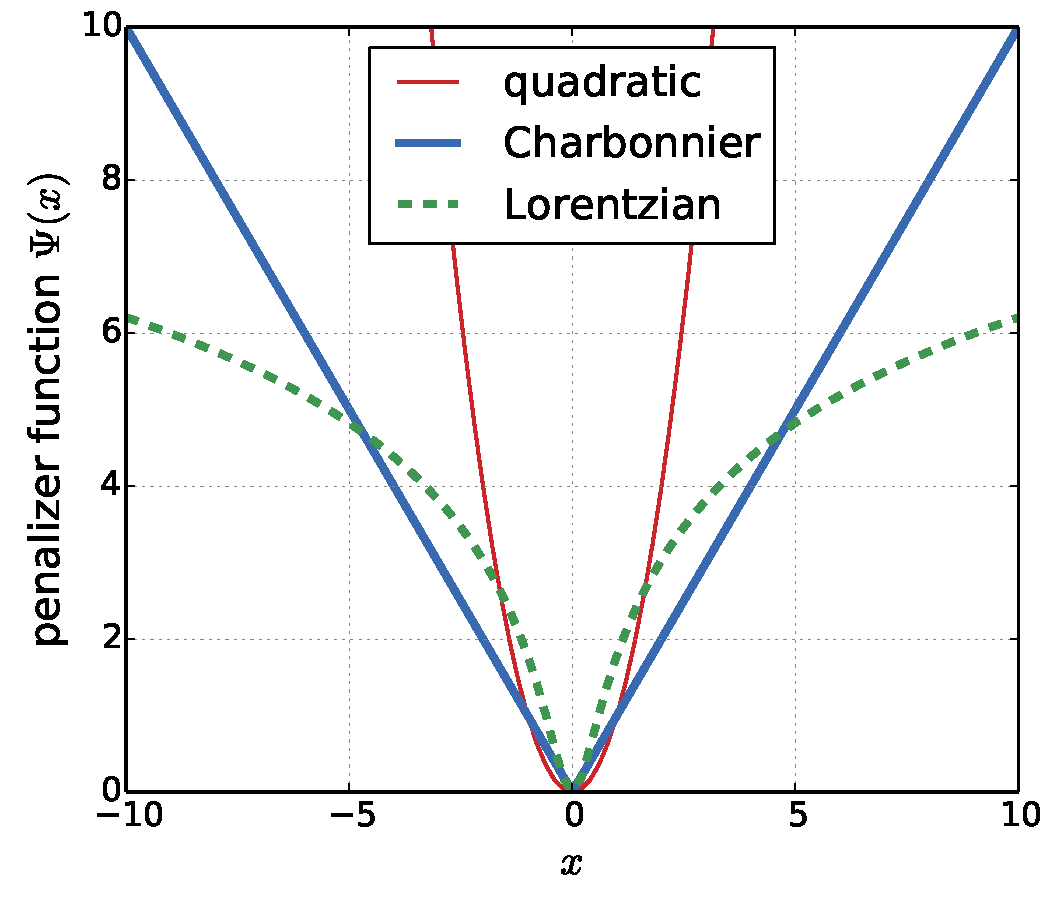
\includegraphics[width=0.45\textwidth]{figures/robust_functions.pdf} 
  }  
  \caption{Comparison between penalising functions: quadratic, Charbonnier and Lorentzian.}
  \label{fig:2_penalisers}
\end{figure*}
For our purpose we choose a penaliser function, which is a differentiable variant of $L_1$-norm \cite{Brox04}:
$$ \Psi_R(x) = \sqrt{x^2 + \epsilon^2},$$
where $\epsilon$ is a small positive constant used to avoid a problem of division by zero after differentiation step.

An example of a robust data term for brightness constancy assumption (see Section \ref{brightness_constancy_assumption}) is given by:
$$ D_{R}(I,\textbf{w}) = \Psi_R ( \nabla_{3}^{\top}I\textbf{w}).$$
As a result of such robust modelling the quality of \opticalflow estimation significantly improves \cite{Sun10, Middl, HarmonyFlow}. We perform quantitative and qualitative evaluation of robust settings in the presence of image artifacts in the experimental sections \ref{experiment_robust_data_term_low_contrast} and \ref{experiment_robust_data_term_low_contrast}.
%\todo{Mention about low contrast here?}

\subsubsection{Joint and Separate Modeling}
\label{joint_and_separate}

In the case when multiple data constraints are used, as we discussed in Section \ref{assumptions_on_multiple_image_features}, an important aspect is how to penalize individual data terms.
One approach is to apply a single penalty function on both data constraints.  On the example of combined brightness and gradient data constancy assumptions this  can be illustrated as:
$$ D_{joint}(I,\textbf{w}) = \Psi_R (\beta_{1}( \nabla_{3}^{\top}I \textbf{w}) + 
\beta_{2} (\nabla_{3}^{\top}I_{x}\textbf{w} + \nabla_{3}^{\top}I_{y}\textbf{w})). $$

Evidently, it is not necessary that both constraints should be satisfied at the same time for all data points. As it was previously shown, brightness constraint fails in regions where illumination changes and gradient constraint is sensitive to noise. However, the deviations from both constraints are penalized jointly. Note, that weight parameters $ \beta_1, \beta_2$ are coupled as an argument of the penalty function, which slightly changes its mathematical formulation. 
 
In the work of \cite{Bruhn05b} the authors introduced a concept of \textit{separate robustification}.
Such strategy takes into account all the data constraints independently and allows to use a different penalty function for each counterpart. Using this approach, we rewrite the combined constraint as:
$$ D_{sep}(I,\textbf{w}) =  \beta_{1}\Psi_{R_1}( \nabla_{3}^{\top}I \textbf{w}) + 
\beta_{2} \Psi_{R_2} (\nabla_{3}^{\top}I_{x}\textbf{w} + \nabla_{3}^{\top}I_{y}\textbf{w}). $$
 
Following the performance analysis from the literature \cite{Bruhn05b, HarmonyFlow}, if multiple image features are used to impose data constancy assumption we choose a separate robustification strategy. Such setting is more flexible and provides better results in most cases.

\subsubsection{Combined Local-Global Approach}
\label{clg}

A useful approach to improve robustness of \opticalflow methods on noisy data is to consider the information not only from a particular data point, but also in a local neighbourhood. The modified data term would then impose a constancy assumption within a fixed region. Such constraint strongly resembles an original \opticalflow method by Lucas and Kanade \cite{LucasKanade81}. In the work of \cite{Bruhn02} so-called \textit{combined local-global} (CLG) approach was introduced. The name highlights the fact that such technique combines the local information for the modelling of data term and provides dense results of global variational methods. 

It is reasonable to weight contributions within a local region according to a distance from the central location (e.g. using weighted least squares fit). In \cite{Bruhn02} it is presented how this approach could be incorporated for the construction of robust data terms. For brightness constancy assumption a least square fit is given by convolution with a Gaussian function: 
$$ D_{CLG}(I,\textbf{w}) =  K_{\rho} \ast (\nabla_{3}^{\top}I\textbf{w})^2, $$
with the standard deviation $\rho$. The standard deviation parameter is also called \textit{integration scale} \cite{Bruhn02}, since it regulates the size of spatial region which is taken into account. 

This approach is not frequently used in the recent works since in cases when a high quality, noise-free data is available it could provide more blurry flow results. However, the combined local-global approach can lead to significant improvements for images which are highly degraded by noise \cite{Bruhn02, Bruhn05a}. We present numerical experiments on noisy data and discuss the usefulness of the local-global approach in the experimental section \ref{experimen_combined_local_global_approach}.


\subsubsection{Normalization of Data Terms}
\label{normalization}

To provide additional robustness in unreliable regions influenced by noise or artifacts it is possible to further adjust the data term.  In the recent work of  \cite{HarmonyFlow} the authors used the ideas presented in \cite{Simoncelli91, Lai98} to perform \textit{normalization} of data constraints. One can show that image locations with large gradient and smooth regions are weighted differently \cite{HarmonyFlow}. As a result, high-gradient features provide more contribution to overall energy of the data term and thus largely influence the estimation of optical flow. Such behaviour can be undesired since high image gradient may be caused by noise or artifacts.
Following \cite{Lai98, HarmonyFlow} the original data constraint can be normalized by a factor:
$$n =  \frac{1}{|\nabla_2 I(x,y,t)|^2 + \eta} , $$
where positive parameter $\eta$ avoids division by zero and controls the normalisation process depending on the noise scale. 

%The influence of normalization is shown in Figure \ref{fig:data_normalization}. 

%\begin{figure*}[ht]
%  \centerline{
%    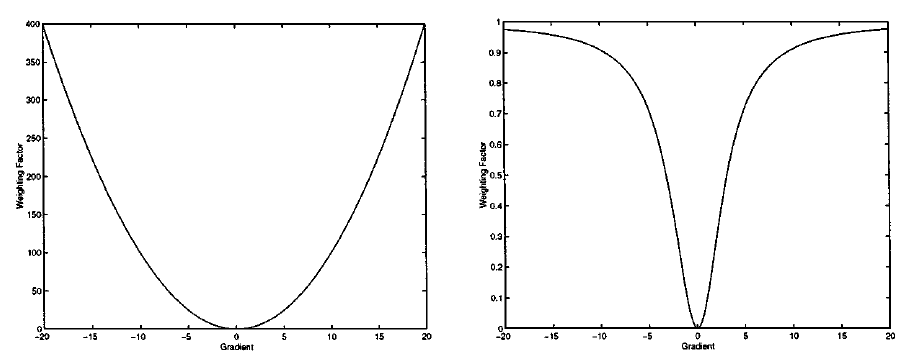
\includegraphics[scale = 0.4]{figures/data_normalization.PNG} 
%  }  
%  \caption{\todo{Remake image}Comparison between the original and normalized data constraint.  \textbf{Left:} Original quadratic weighting. \textbf{Right:} Normalized weighting. }
%  \label{fig:data_normalization}
%\end{figure*}

After the normalization procedure the resulting data term is still convex and can be easily incorporated in our variational computation scheme. The normalized brightness constancy constraint is given by:
$$ D_{norm}(I,\textbf{w}) = n (\nabla_{3}^{\top}I\textbf{w})^2.$$

For low contrast and noisy X-ray images the use of normalized data terms can be especially beneficial. We discuss the influence of proposed correction procedure, as well as choice of the appropriate $\eta$ parameter on various amounts of noise in Section \ref{experiment_normalization_data_term}.

\subsubsection{Refinement Model}
\label{refinement}

In the work of \cite{Xu10} authors proposed to explicitly model occlusions (or other data outliers) and reduce the influence of data term in these regions.  First, a motion estimation is performed using appropriate model assumptions, then a confidence map is constructed using an occlusion detection. Then, a second run of optical flow algorithm is done using occlusion-aware refinement:
$$E_{refine}(I, \textbf{w}) = \int_{\Omega}{(c(\textbf{x}) \cdot \: D(I, \textbf{w}) + \alpha   S(I, \textbf{w})) \: \text{d}\Omega},$$
where $c(\textbf{x})$ is a confidence map, which downweights the contribution of data constraint for unreliable image regions, $D(I,\textbf{w})$ is a data constraint and $S(I, \textbf{w})$ regulates the smoothness properties of the flow field. 

We discuss various approaches for the estimation of confidence maps in Section \ref{confidence_measures}.


%-------------------------------------
\subsection{Smoothness Assumptions}
\label{smoothness_assumptions}
%-------------------------------------


As it was mentioned previously, assuming constancy constraints based only on local image data is not sufficient to uniquely find a solution for optical flow. In order to overcome the aperture problem additional assumptions about the  flow field itself are employed. The first idea to impose such assumptions goes back to the seminal work of Horn and Schunck \cite{HornSchunck81}. Smoothness constraints allow a \textit{filling-in} \cite{Weickert00b} of the flow information from the adjacent regions at image locations where no unique correspondence can be determined. Most of the approaches impose smoothness constraint by penalizing the magnitude of the flow gradient. 
According to the specific properties of the smoothness one may distinguish between \textit{homogeneous}, \textit{isotropic} and \textit{anisotropic} smoothness. For a more detailed description of various models we refer the reader to the work of \cite{Weickert00b}.

\subsubsection{Homogeneous Smoothness}
\label{homogeneous_smoothness}

The original method of Horn and Schunck \cite{HornSchunck81} introduces smoothness assumption by penalizing magnitude of the flow gradient:
$$ S_{HS}(u,v) = u_{x}^2 + u_{y}^2 + v_{x}^2 + v_{y}^2 = |\nabla_2 u|^2 + |\nabla_2 v|^2,$$
where $|\textbf{f}| = \sqrt{f^2_x + f^2_y}$ is a spatial magnitude and $\nabla_2 = (\partial_{x}, \partial_{y})$ denotes a spatial gradient.
This \textit{homogeneous} regularization requires uniformly smooth flow fields and does not adapt to any supplementary information about image data and the flow field. Assuming that depicted objects may move differently from the background or with respect to each other it is evident that such constraint can hardly be fulfilled. Therefore, smoothness assumptions which allow to model discontinuities more thoroughly are required.

\subsubsection{Image-Driven Smoothness}
\label{image_driven}

In order to take into account motion discontinuities one may assume that the flow field coincides with the boundaries of moving object, thus the smoothness degree can be adjusted according to image edges  \cite{Nagel86, Alvarez99}. To implement this approach one can multiply the original smoothness term by a scalar weighting function $g(x)$ that decreases on image edges \cite{Schnorr93, Alvarez99}. One possibility for such function is:
$$ g(x) = \frac{1}{2 \sqrt{x + \epsilon}}, $$
where $\epsilon$ is a small positive constant used to avoid a problem of division by zero.

The obtained \textit{image-driven} smoothness term is given by:
$$ S_{image}(I,u,v) = g(|\nabla I|^2)(|\nabla u|^2 + |\nabla v|^2), $$
where the magnitude of the spatial gradient $|\nabla I|$ is used to identify image edges \cite{Weickert00b}. It should be noted, that such smoothness term is isotropic, since it treats all directions in image gradients in the same manner. To enhance the smoothing process along image edges, and suppress across them one can use an anisotropic image-driven approach \cite{Nagel86}. 

Despite the fact that image-driven regularization provides sharp edges on the boundaries of moving object, it is prone to errors if the image gradient does not correspond to the actual flow discontinuities. For instance, this occurs in highly textured regions. Image noise is another challenge for this method, which causes the smoothness value to be adjusted to noise variations. In both cases image-driven approaches produce oversegmentation artifacts in the computed flow field. 

\subsubsection{Flow-Driven Smoothness}
\label{flow_driven}

To preserve motion discontinuities the smoothness can be adapted to the unknown flow field. In this case the smoothness is reduced at flow edges described by the flow gradient \cite{Shulman89, Schnorr94}.
The regularization based on the \textit{flow-driven} approach is thus given by:
$$ S_{flow}(u,v) = \Psi_{S}(|\nabla u|^2 + |\nabla v|^2), $$
where the smoothness penalty function reads  $\Psi_{S}(x) = \sqrt{x + \epsilon}$ and corresponds to the total variation (TV) regularization \cite{ROF92}.

In comparison to image-driven method the flow-driven approach provides less strict estimation of flow edges on the boundaries of the moving objects. However, for high-texture or noisy data the flow-driven approach is more robust and outperforms image-driven flow regularization \cite{Brox04, Papenberg06, Wedel09}.   



%\subsubsection{Anisotropic Smoothness}
%\label{anisotropic_driven}
%
%\comment{Info from Bruhn thesis}
%
%\change{From: \cite{Middl}. In (10) the weighting function is isotropic, treating all directions equally. A variety of approaches weight the smoothness
%prior anisotropically. For example, Nagel and Enkelmann
%(1986) and Werlberger et al. (2009) weight the direction
%along the image gradient less than the direction orthogonal
%to it, and Sun et al. (2008) learn a Steerable Random
%Field to define the weighting. Zimmer et al. (2009) perform
%a similar anisotropic weighting, but the directions are defined
%by the data constraint rather than the image gradient.}
%
%\change{From: \cite{HarmonyFlow} An anisotropic counterpart that also exploits the
%directional information of image discontinuities was introduced by Nagel and Enkelmann (1986). Their method regularises the flow field along image edges but not across them.
%As noted by Xiao et al. (2006), this comes down to convolving the flow field with an oriented Gaussian where the orientation is adapted to the image edges.}
%
%\change{From: Bruhn. Flow-driven regularisers take into account discontinuities of the unknown flow field u
%by preventing smoothing at or across flow discontinuities. If the resulting diffusion process
%uses a scalar-valued diffusivity that only depends on |ru|2 := |ru1|2 + |ru2|2, it
%is an isotropic process [Sch94b]. Cases where also the direction of ru1 and ru2 matters
%are named anisotropic [WS01a]. Flow-driven regularisers lead to nonlinear diffusion
%processes.}
%
%For more in-depth qualitative and quantitative comparison of isotropic and anisotropic settings we refer the reader to the work of [WS01a] and Bruhn thesis.


\subsubsection{Spatial-Temporal Smoothness}
\label{spatial_temporal}

In case if more then two frames are given for the estimation of optical flow, it is reasonable to additionally assume temporal smoothness of the flow fields \cite{Murray87, Black91}. For variational approaches such spatial-temporal smoothness terms were proposed by \cite{Nagel90} and \cite{Weickert2001b}.
Implementation of the spatial-temporal smoothness term is done by the extension of spatial derivatives to the spatial-temporal dimension:
$$ S_{temp}(u,v) = u_{x}^2 + u_{y}^2 + u_{t}^2+ v_{x}^2 + v_{y}^2 + v_{t}^2 = |\nabla_3 u|^2 + |\nabla_3 v|^2,$$
where $\nabla_3 = (\partial_{x}, \partial_{y}, \partial_{t})$ denotes the spatial-temporal gradient.


The usage of temporal information provides a significant improvement for the estimation of optical flow \cite{Brox04, HarmonyFlow}. In the case when stationary regions are corrupted by noise the temporal regularization helps to smooth noise contributions and correctly estimate zero flows. This property of spatial-temporal smoothness is especially useful if one is interested in separation between moving objects and a static background, i.e. for motion-based segmentation.
For moving objects the applicability of the temporal smoothness depends on the type and magnitude of displacements. In the case of small, linear displacements the extension to the temporal domain will not cause problems since the influence of spatial and temporal smoothness will be approximately equal. However, in the presence of fast motion large discontinuities in a temporal direction may emerge. To appropriately handle them a number of strategies can be used. One way would be to use the coarse-to-fine computation scheme which allows to solve for large displacements. We describe this technique in details in Section \ref{coarse_strategy}. Another option would be to employ discontinuity preserving smoothness terms using robust penalty function presented in Section \ref{flow_driven}. This approach will result into a joint spatial-temporal discontinuity preserving smoothness term:
$$ S_{flow-temp}(u,v) = \Psi_{S}(|\nabla u|^3 + |\nabla v|^3), $$
where $\Psi_{S}(x) = \sqrt{x + \epsilon}$  and  $\nabla_3 = (\partial_{x}, \partial_{y}, \partial_{t})$.

An important aspect for modeling temporal smoothness is a number of time frames used to impose constraints in temporal direction. In the works of \cite{BruhnThesis}, \cite{HarmonyFlow} it was shown that increasing the number of frames significantly improved the results. However, it was also observed that there is an upper limit after which there is no longer an improvement in the result. The usage of both spatial and temporal information about the flow field allows to decrease the optimal value for smoothness parameter, which result in a sharper flow edges. Additionally, it is reasonable to apply presmoothing step described in Section \ref{image_smoothing} also in temporal direction \cite{BruhnThesis}. The temporal smoothness parameter should be chosen according to constancy of the motion in time and amount of noise.
In general, spatial-temporal smoothness provides a robust approach to compute the optical flow, especially for noisy or corrupted data.



\subsubsection{Adaptive Smoothness}
\label{adaptive_smoothness}


The smoothness term can be further adapted using a number of different strategies.
One approach would be to use a weighting function based on segmented masks representing particular data objects. Such objects could be identified during the optical flow computation or can be pre-labeled using an a-priori knowledge. An example of such masks could be a reduction of smoothness weight on the boundary of closely moving objects, which may improve the separation between them. Another example corresponds to the case when the motion in separate regions expected to exhibit different properties.

The adaptive variant of the smoothness term is then given by:
$$ S_{adapt}(I,u,v) = \alpha_{S_{i}}(|\nabla u|^2 + |\nabla v|^2), $$
where $\alpha_{S_{i}}$ represents the smoothness parameter inside or around the segment $S_{i}$.

Another strategy is to adapt the smoothness according to the computation procedure.
In \cite{HarmonyFlow} authors proposed to adjust the smoothness weight on each level of multiscale computation of optical flow. One may note, that on coarser image levels the data term provides less details resulting from smoothing properties of the downscaling procedure. In this case it makes sense to increase the influence of the smoothness term. This can be done by adjusting the flow regularization according to the warping computation level $k$:
$\alpha(k) = \frac{\alpha}{\eta^k},$
where  $\eta$ is a downscaling factor.



\subsubsection{Joint Image and Flow Driven Smoothness}
\label{image_flow_smoothness}


As it was discussed in Sections \ref{image_driven} and \ref{flow_driven} both image- and flow-driven smoothness approaches have their advantages and drawbacks. To improve the performance of optical flow estimation it makes sense to combine the advantages of both methods to obtain precise motion discontinuities and avoid oversegmentation problems in highly textured image regions. 
The first idea which achieves that was presented in \cite{Sun08}. In this work the smoothness direction is adapted to image edges and smoothing amount to the flow gradient. In \cite{HarmonyFlow} the authors presented a more general approach, which they call \textit{complementary smoothness term}.  Such approach regulates the smoothness direction according to the data constraint, which could be different from information given by image gradients. As a result the smoothness is reduced in the direction where data constraint provides useful information and increased in regions where data constraint is vanished.  





%-------------------------------------
\subsection{Measures of Confidence}
\label{confidence_measures}
%-------------------------------------

In Section \ref{quality_measures} we have described measures for quantitative evaluation of \opticalflow algorithms in the case when the ground truth result is known. In this section we discuss measures to check the reliability of optical flow based only on the computed flow field and initial image data. 
     
Until the recent works of \cite{Sun10, HarmonyFlow} only little attention was dedicated to the application of confidence measures for \opticalflow methods.  
These measures can allow us to determine errors in the computed flow fields caused by artifacts. Moreover, we may use these measures to evaluate the quality of the computed result and automatically optimize the model parameters for the \opticalflow computation.  


\subsubsection{Gradient-based Measure}

The first confidence measure for variational \opticalflow methods was presented by \cite{Barron94}.
It was proposed to relate the quality of the flow estimation with the image gradient, since as it was discussed in Section \ref{general_model} the correspondence problem can only be solved if there is enough information provided by the local image gradient. The confidence measure based on image data is thus given by:
$$ C_{gradient}(\textbf{x}) = |\nabla I(\textbf{x})|. $$
Clearly, this measure does not take into account any dynamical information and assumes only local image data. Additionally, this measure is not capable to evaluate global optical flow approaches which use additional smoothness term to overcome the aperture problem. Moreover, the variations in image brightness can be caused by noise or artifacts. These drawbacks make image-based confidence measure not well suited for the evaluation of optical flow estimation.


\subsubsection{Energy-based Measure}
\label{energy_based_measure}

In the work of \cite{Bruhn06, ErshovThesis} the authors presented an intuitive way to evaluate the quality of variational optical flow methods based on energy minimization. 
Since during minimization  procedure such functionals penalize deviations from model assumptions, it is very natural to consider such deviations as a confidence measure. 

For the case of method of Horn and Schunck the energy-based confidence measure for a pixel \textbf{x} reads:
$$ C_{energy}(\textbf{x}) = \frac{1}{(\nabla_{3}^{\top}I(\textbf{x})\textbf{w})^2 + \alpha ( |\nabla_2 u(\textbf{x})|^2 + |\nabla_2 v(\textbf{x})|^2)}. $$

At this point one may consider to evaluate energy contributions from both data and smoothness terms jointly or, alternatively, evaluate only the data term which constitutes the optical flow problem, i.e. correspondence between pixels (see Section \ref{data_constancy_error}).  
In the presence of artifacts or other data outliers the model assumptions are violated, which results in a high values of energy in those regions.  

As it was discussed in \cite{Bruhn06} energy-based confidence measures have a number of advantages: 1) it is based on the same assumptions as the computational model 2) it is general and could be extended or modified for a particular optical flow model 3) it does not require additional parameters.


\subsubsection{Data Constancy Error}
\label{data_constancy_error}

A similar concept to the energy-based confidence measure is a data constancy error, which evaluates only the data constraint. For the case of brightness constancy assumption, the confidence measure for a pixel \textbf{x} reads:

$$ C_{data}(\textbf{x}) = (I(\textbf{x} + \textbf{w}, t+1) - I(\textbf{x}, t)). $$

This measure shares the same set of advantages as the energy-based confidence measure, as it is also directly based on an optical flow model.


\subsubsection{Motion Uniqueness Criteria}
\label{motion_uniqueness_criteria}

Another approach to evaluate the computed flow field is to examine its spatial distribution. 
We assume that if the motion is applied (source image is warped towards the target image) all pixels should still be uniformly distributed \cite{Brown03, ErshovThesis, Xu10}. However, in the presence of data outliers or problems with appearing and disappearing information the flow vectors could point to nearly the same position. Such multiple pixels mapping could indicate a location of unreliable motion estimation. This idea is illustrated in Figure \ref{fig:4_uniqueness}. 

\begin{figure*}[ht]
  \centerline{
    \mbox{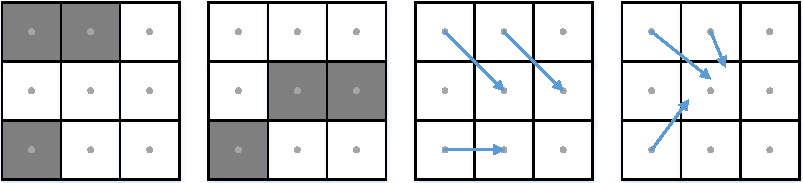
\includegraphics[width=0.9\textwidth]{figures/fig_22_p42.pdf}} 
  }
  \caption[Flow Uniqueness.]{Flow uniqueness criteria. \textbf{Left:} First image frame. \textbf{Middle Left:} Second image frame. \textbf{Middle Right:} One-to-one correspondence. Pixels are mapped to uniformly distributed positions. \textbf{Right:} Pixels are mapped nearly to the same position, indicating a  sink in a vector field.}
  \label{fig:4_uniqueness}
\end{figure*}

In order to implement this approach we count a number of arrived pixels $\textbf{x}+\textbf{u}(\textbf{x})$  to the target image position $\textbf{x}$ . In order to handle real-valued displacements we redistribute contributions from neighboring flow vectors according to their distance to the target pixel location. The confidence measure based on motion uniqueness mapping is then expressed by:
$$ C_{unique}(\textbf{x}) = \frac{1}{|1 - count(\textbf{x})| + \epsilon}, $$
where $\epsilon$ is a small posotive contstant to avoid a division by zero problem.
The deviations from the one-to-one mapping will be captured and the confidence degree will be reduced.


        
\subsubsection{Forward-Backward Check}
\label{forward_backward_check}

A common way to ensure consistency of a motion field solution in the presence of occlusions is to perform a so-called \textit{forward-backward check} (or \textit{cross-checking}) \cite{Chang91, Fua93, Brown03}. In this approach we assume that the flow field computed in forward (from  $I(\textbf{x}, t)$ to $I(\textbf{x}, t+1)$) and the backward direction is equal, but opposite:

%$$ u^{forw}_{ij} = - u^{back}_{i+ u^{forw}_{ij}, j +  v^{forw}_{ij}} $$   
%$$ v^{forw}_{ij} = - v^{back}_{i+ u^{forw}_{ij}, j +  v^{forw}_{ij},} $$
%where $\textbf{w}^{fw}$ and $\textbf{w}^{bw}$ is a flow field computed in forward and backward %direction respectively.

$$ \textbf{w}^{f}(\textbf{x}) = - \textbf{w}^{b}(\textbf{x} + \textbf{w}^{f}(\textbf{x}))$$   
where $\textbf{w}^{f}$ and $\textbf{w}^{b}$ is a flow field computed in a forward and a backward direction respectively.

In the case of occlusions or other image artifacts, forward and backward vectors do not match, which could be exploited to identify problematic regions. For the consistency based confidence measure we estimate the magnitude of the difference vector between forward and backward flow vectors:
$$ |\Delta \textbf{w}(\textbf{x})| = \sqrt { \left ( \textbf{w}^{f}(\textbf{x}) + \textbf{w}^{b}(\textbf{x} + \textbf{w}^{f}(\textbf{x})) \right )^2  }$$

%$$ |\Delta \textbf{w}_{ij}| = \sqrt { \left (u^{forw}_{ij} + u^{back}_{i+ u^{forw}_{ij}, j +  v^{forw}_{ij}} \right )^2 + \left (v^{forw}_{ij} + v^{back}_{i+ u^{forw}_{ij}, j +  v^{forw}_{ij}} \right )^2 }$$

\begin{figure*}[h]
  \centerline{
    \mbox{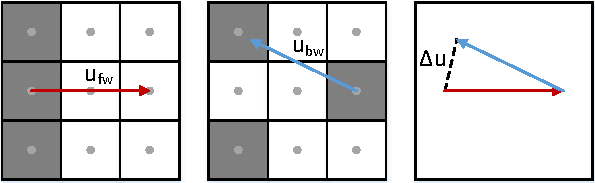
\includegraphics[width=0.7\textwidth]{figures/fig_23_p43.pdf}} 
  }
  \caption[Forward-Backward check method]{Forward-Backward check method. \textbf{Left:} First image frame with the forward flow vectors. \textbf{Middle:} Backward flow vectors for interchanged images. \textbf{Right:} Discrepancy vector between forward and backward displacement vectors.}
  \label{fig:4_forw_back}
\end{figure*}

The idea for forward-backward check approach is illustrated in Figure \ref{fig:4_forw_back}. 

As a result we consider pixels, where consistency check failed as locations with a low confidence value:
$$ C_{consist}(\textbf{x}) = \frac{1}{|\Delta \textbf{w}(\textbf{x})| + \epsilon}. $$
 We will employ this measure in the section dedicated to analysis of temporal changes in metal foams of various kind in the application Section \ref{application_foams}. 


\subsubsection{Optimal Prediction Principle}
\label{optimal_prediction_principle}

Recently, in \cite{HarmonyFlow} the authors proposed a confidence measure based on the principle of optimal prediction (OPP). It states that the flow field computed with optimal model parameters allows for the best flow prediction for the next image frames. For this, one assumes that the objects are moving with a constant velocity and linear trajectory. 
This can be implemented by scaling the flow vector by 2.  
In order to estimate the prediction quality a data term between the first and the third frame is evaluated. The resulting data constancy error (DCE) measure is given by: 

$$ C_{predict}(\textbf{x}) = (I(\textbf{x} + \textbf{2w}, t+2) - I(\textbf{x}, t)). $$

Despite its simplicity, confidence measure based on the optimal prediction principle gives good results \cite{HarmonyFlow}. The only drawback is a restriction imposed by the assumption of temporally constant flow field, which can be frequently violated.

We test the performance of automated confidence measures and give conclusions regarding their use in the experimental section \ref{exp_confidence_evaluation}.




%%-------------------------------------
%\subsection{Advanced Techniques}
%%-------------------------------------
%
%\comment{Which advanced methods to show?}
%\comment{Why these methods are not implemented then? Think about how to explain}
%
%\begin{itemize}
%  \item My median data term + selective data term
%\end{itemize}
%
%
%\subsubsection{[OPTIONAL] Fusion of Multiple Results}
%
%\todo{Read Fusion Flow (Lempitsky et al. 2008)}
%
%\change{From: \cite{Middl}. Fusion Flow (Lempitsky et al. 2008) uses a sequence
%of binary graph-cut optimizations to refine the current
%flow estimate by selectively replacing portions with one
%of the candidate solutions.}
%
%\comment{2 approaches: joint minimization of different models, separate minimization and merging}
%

%-------------------------------------
\subsection{Generalization to 3D Optical Flow}
\label{extension_3d}
%-------------------------------------

In order to apply \opticalflow methods on tomographic data, the extension from the 2D variational model into a 3D model should be performed.
This step is done in a straightforward way by including an additional spatial dimension. The advantages for 3D optical flow are discussed in the section, describing computed tomography experiments (see Section \ref{computed_tomography}).

%\begin{figure*}[h]
%  \centerline{
%    \mbox{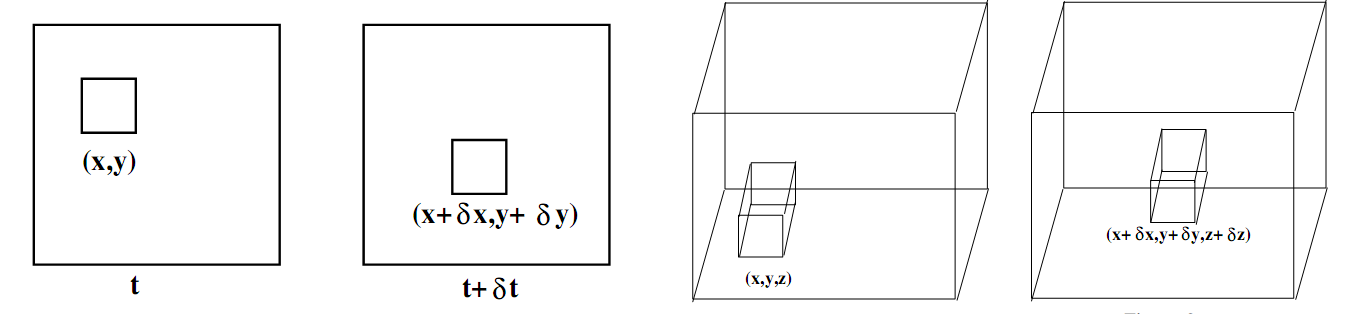
\includegraphics[scale = 0.3]{figures/2D_3D.png}} 
%  }
%  \caption[2D_3D]{Extension of optical flow methods for 3D. \textbf{Left:} Image model for 2D.  \textbf{Right:} Image model for 3D.}
%  \label{fig:2d_3d}
%\end{figure*}

The 2D variational \opticalflow model using the flow-driven smoothness approach (Section \ref{flow_driven}) is given by:
$$ E_{2D}(u,v) = \int_{\Omega_{2}}{(I(x+u,y+v,t+1) - I(x,y,t))^2 + \alpha \Psi(|\nabla_{2}u|^2 + |\nabla_{2}v|^2) \text{d}x \text{d}y}. $$
For a volume image $I(x,y,z,t)$, where $(x,y,z)$ are the voxel coordinates within an image domain $ \Omega_{3} \subset \mathbf{R}^3$, the extension to the 3D variational model reads:
\begin{eqnarray}
E_{3D}(u,v,w) &=& \int_{\Omega_{3}}{}(I(x+u,y+v, z+w, t+1) - I(x,y,z,t))^2 + \nonumber \\  
 &+& \alpha \: \Psi(|\nabla_{3}u|^2 + |\nabla_{3}v|^2 + |\nabla_{3}w|^2) \text{d}x \text{d}y \text{d}z. \nonumber
\end{eqnarray}

It is important to mention that some of the problems of 2D optical flow estimation disappear after the extension into a 3D domain. For example, there are no problems related to the projection geometry, such as occlusions between moving objects or divergent motion due to the perspective change.

As a drawback, solving 3D optical flow problem is a resources demanding task. It requires both large memory consumption and intense computational power. We further discuss performance aspects in Chapter \ref{performance} we describe a number of efficient computation schemes and present high-performance implementation of 3D optical flow methods on GPUs. 

\todo{Put examples of 3D data terms}  


%--------------------------------------------------------
\section{Numerical Solution}
%--------------------------------------------------------

In this section we explain how a variational optical flow model can be solved numerically. For this purpose we introduce a minimization procedure and iterative methods. We also discuss important implementation aspects, such as discretization and a derivatives approximation. In the first part of the section we derive underlying equations assuming small displacements between image frames.  Then we present an extension of the energy functional and its minimization procedure which allows to handle large displacements. To shorten the derivation of the corresponding formulas we assume 2D images. The extension to 3D domain can be performed in similar manner.   


\subsection{Minimization Procedure}
\label{minimization_procedure}

In the previous chapter we have discussed the construction of a variational energy functional. Next, our aim is to  find such a displacement field $u(x,y)$ and $v(x,y)$ which minimizes deviations from the model assumptions.

According to calculus of variations \cite{elsgolts62}, the minimum of the convex variational functional of the general form:
$$ E(u,v) = \int_{\Omega_{2}}{F(x,y,u, v, u_x, u_y, v_x, v_y})\text{d}x \text{d}y. $$
can be found at the location where its first-order derivatives vanish.
Such coupled differential equations are called \textit{Euler-Lagrange equations} and given by:
\begin{eqnarray}
F_u - \frac{\partial}{\partial x}F_{u_x} - \frac{\partial}{\partial y}F_{u_y} &=& 0 \\  \nonumber 
F_v - \frac{\partial}{\partial x}F_{v_x} - \frac{\partial}{\partial y}F_{v_y} &=& 0 
\label{eq:euler}	
\end{eqnarray}
with reflecting Neumann boundary conditions $\textbf{n}^\top \nabla u = 0$ and $\textbf{n}^\top \nabla v = 0$, where $\textbf{n}$ is a normal vector.


We show an example of minimization procedure on a flow-driven optical flow model with brightness constancy assumption. First, we calculate partial derivatives with respect to the unknown functions $u$ and $v$:
$$ F_u = 2 I^2_x u + 2 I_x I_y v + 2 I_x I_t $$ 
$$ F_v = 2 I_y I_x u + 2 I^2_y v + 2 I_y I_t $$
$$ F_{u_x} = 2 \alpha \: \Psi'(|\nabla u|^2 + |\nabla v|^2) \: u_x$$ 
$$ F_{u_y} = 2 \alpha \: \Psi'(|\nabla u|^2 + |\nabla v|^2) \: u_y$$
Embedding these terms into the Euler-Lagrange equations (\ref{eq:euler}) we obtain:
$$ I^2_x u + I_x I_y v + I_x I_t - \alpha \: \textrm{div} (\Psi'(|\nabla u|^2 + |\nabla v|^2) \cdot \nabla u ) = 0, $$
$$ I_y I_x u + I^2_y v + I_y I_t - \alpha \: \textrm{div} (\Psi'(|\nabla u|^2 + |\nabla v|^2) \cdot \nabla v ) = 0. $$
Solving this coupled system of equations with respect to the unknown displacement functions $u$ and $v$ gives us the minimum of our energy functional. 

\subsection{Discretization}
\label{discretization}

To solve Euler-Lagrange equations numerically we should perform a discretization procedure. We consider the unknown functions $u(x,y,t)$ and $v(x,y,t)$ on a rectangular image with the grid size of $h_x$ in $x$-direction and $h_y$ in $y$-direction. The values $u_{ij}$ and $v_{ij}$ denote the approximation of functions $u(x,y)$ and $v(x,y)$ at a pixel position $(i,j)$ with $i = 0 \ldots N-1, j=0 \ldots M-1$, where $N$, $M$ indicate image dimensions. 

In order to represent image derivatives we must assume a particular approximation of the differential operator. 
Second order approximations of the spatial image derivatives using central differences are given by:
$$ \left[ I_x \right]_{i,j} = \frac{I_{i+1,j,t} - I_{i-1,j,t} }{2 h_x} $$
$$ \left[ I_y \right]_{i,j} = \frac{I_{i,j+1,t} - I_{i,j-1,t} }{2 h_y} $$

To improve the accuracy of derivatives approximation one may also use fourth order approximations:
$$ \left[ I_x \right]_{i,j} = \frac{-I_{i+2,j,t} +  8  I_{i+1,j,t} - 8 I_{i-1,j,t} + I_{i-2,j,t} }{12 h_x} $$
$$ \left[ I_y \right]_{i,j} = \frac{-I_{i,j+2,t} +  8  I_{i,j+1,t} - 8 I_{i,j-1,t} + I_{i,j-2,t} }{12 h_y} $$

For further improvement with respect to noise it is common to use a temporal averaging of spatial derivatives \cite{Sun10, HarmonyFlow}.
For the second order central difference such a temporal averaging is given by:
$$ \left[ I_x \right]_{i,j} = \frac{(I_{i+1,j,t+1} - I_{i-1,j,t+1}) + (I_{i+1,j,t} - I_{i-1,j,t})  }{4 h_x} $$
$$ \left[ I_y \right]_{i,j} = \frac{(I_{i,j+1,t+1} - I_{i,j-1,t+1}) + (I_{i,j+1,t} - I_{i,j-1,t}) }{4 h_y} $$


To compute temporal derivatives we choose a forward difference:
$$ \left[ I_t \right]_{i,j} = \frac{I_{i,j,t+1} - I_{i,j,t}}{h_t},$$
where time step $h_t$ is chosen to be equal to 1.0.

We proceed with the discretization of others terms such as  $\textrm{div}(\Psi'(|\nabla u|^2 + |\nabla v|^2) \nabla u)$. 
Additionally to the second-order derivative approximation, we can also employ the discretization approach based on nested central differences with the halved grid sizes  $\frac{1}{2}h_x$ and $\frac{1}{2}h_y$.
Using this strategy the term $\textrm{div}(\Psi'\nabla u)$ can be expressed as: 
\begin{eqnarray}
\textrm{div}(\Psi'\nabla u) &=& (\Psi' u_x)_x + (\Psi' u_y)_y \nonumber \\
&=& \frac{ (\Psi' u_x)_{i + \frac{1}{2},j} - (\Psi' u_x)_{i - \frac{1}{2},j} }{2 (\frac{1}{2} h_x)} + 
\frac{ (\Psi' u_y)_{i,j + \frac{1}{2}} - (\Psi' u_y)_{i,j- \frac{1}{2}} }{2 (\frac{1}{2} h_y)} \nonumber \\
&=& \frac{\frac{\Psi'_{i+1,j} + \Psi'_{i,j}}{2} \left ( \frac{u_{i+1,j} - u_{i,j} }{2 (\frac{1}{2} h_x)} \right )   - \frac{\Psi'_{i,j} + \Psi'_{i-1,j}}{2}  \left (\frac{u_{i,j} - u_{i-1,j}}{2 (\frac{1}{2} h_x)} \right ) }  {2 (\frac{1}{2} h_x)} \nonumber \\
&+& \frac{\frac{\Psi'_{i,j+1} + \Psi'_{i,j}}{2} \left (  \frac{u_{i,j+1} - u_{i,j}}{2 (\frac{1}{2} h_y)} \right ) - \frac{\Psi'_{i,j} + \Psi'_{i,j-1}}{2} \left ( \frac{u_{i,j} - u_{i,j-1}}{2 (\frac{1}{2} h_y)} \right ) } {2 (\frac{1}{2} h_y)} \nonumber \\
 &=& \frac{\Psi'_{i+1,j} + \Psi'_{i,j}}{2} \left( \frac{u_{i+1,j} - u_{i,j}}{h^2_x} \right ) - \frac{\Psi'_{i,j} + \Psi'_{i-1,j}}{2} \left ( \frac{u_{i,j} - u_{i-1,j}}{h^2_x} \right ) \nonumber \\
 &+& \frac{\Psi'_{i,j+1} + \Psi'_{i,j}}{2} \left( \frac{u_{i,j+1} - u_{i,j}}{h^2_y} \right ) - \frac{\Psi'_{i,j} + \Psi'_{i,j-1}}{2} \left ( \frac{u_{i,j} - u_{i,j-1}}{h^2_y} \right ), \nonumber
\end{eqnarray}
where the nonlinear terms $[\Psi']_{i,j}$ are given by:
$$ [\Psi']_{i,j} = \Psi'(|\nabla u|^2 + |\nabla v|^2) = \Psi'([u_x]^2_{i,j} + [u_y]^2_{i,j} + [v_x]^2_{i,j} + [v_y]^2_{i,j}) $$ 
The discretization of  the term $\textrm{div}(\Psi'\nabla v)$ is done in a similar way.

Finally, after all necessary discretization schemes are introduced we can write down the discrete Euler - Lagrange equations:
$$ [I^2_x]_{i,j} u_{i,j} + [I_x I_y]_{i,j} v_{i,j} + [I_x I_t]_{i,j} - \alpha \: \sum_{l \in x,y} \sum_{(\bar{i}, \bar{j}) \in N_d(i,j)} \frac{[\Psi']_{\bar{i}, \bar{j}} + [\Psi']_{i,j} }{2} \Bigl (\frac{u_{\bar{i}, \bar{j}} - u_{i,j}  } {h^2_d} \Bigr) = 0 $$
$$ [I_y I_x]_{i,j} u_{i,j} + [I^2_y]_{i,j} v_{i,j} + [I_y I_t]_{i,j} - \alpha \: \sum_{l \in x,y} \sum_{(\bar{i}, \bar{j}) \in N_d(i,j)} \frac{[\Psi']_{\bar{i}, \bar{j}} + [\Psi']_{i,j} }{2} \Bigl (\frac{v_{\bar{i}, \bar{j}} - v_{i,j}  } {h^2_d} \Bigr) = 0, $$
where $N_d(i,j)$ denotes neighbor pixels for the position $(i,j)$ in the direction $d \in (x,y)$.

Now, this coupled system of equations has to be solved with respect to the unknown displacements $u_{ij},  v_{ij}$. 

\subsection{Iterative Methods}
\label{iterative_methods}

After the discretization of the Euler-Lagrange equations is performed we obtain a linear system of equations, which can be formulated in the following form:
$$ A \textbf{x} = \textbf{b} $$
To solve it directly, we may invert the system matrix and multiply it by the result vector:
$$ \textbf{x} = A^{-1} \textbf{b} $$
However, for large systems of equations this procedure is computationally expensive. As an alternative, it is possible to decompose the initial matrix $A$ into two terms:
$$ A = A_1 + A_2, $$
and try to approximate the solution iteratively: 
$$ A_1 \textbf{x}^{k+1} = \textbf{b} - A_2 \textbf{x}^k $$
$$ \textbf{x}^{k+1} = A_1^{-1} (\textbf{b} - A_2 \textbf{x}^k)$$
The appropriate choice of matrix $A^{-1}_1$ should be done in such a way, that it is a good approximation to the initial inverse matrix $A^{-1}$. Additionally, it should be easily computable. This matrix splitting strategy is a core idea for a number of iterative methods such as \textit{Jacobi} and \textit{Gau\ss - Seidel methods}. 

\subsubsection{Jacobi method}
\label{jacobi_method}



The Jacobi method is an iterative algorithm to solve a system of linear equations \cite{Saad03}. The system of linear equations $A \textbf{x} = \textbf{b}$ has an unique solution, if the coefficient matrix $A$ contains no zeros on its main diagonal. On each iteration step, one finds the approximate solution for each diagonal element and use it in the next step. The iterative process is then repeated until it converges. 

The Jacobi method can be expressed in a matrix form, using the following decomposition of the initial matrix $A$:
%
\begin{equation}
A = D - L - U,
\end{equation}
%
where $D$, $L$ and $U$ represent the diagonal, strictly lower triangular and strictly upper triangular matrices of $A$, respectively. After the substitution of the decomposed matrix $A$ in the equation $A \textbf{x} = \textbf{b}$, it can be reformulated in the following way::
%
\begin{equation}
D \textbf{x} = (L + U)\textbf{x} + \textbf{b},
\end{equation}
%
and the corresponding iterative solution can be found via:
%
\begin{equation}
\textbf{x}^{k+1} = D^{-1}(L + U)\textbf{x}^{k} + D^{-1}\textbf{b}.
\end{equation}


Using the Jacobi method, the new value of $x_i^{k}$ on the iteration step $k+1$ can be estimated in the following way:
%
\begin{equation}
x_i^{k+1} = \frac{1}{a_{ii}} \left( 
b_i - 
\sum_{j=1, j \neq i}^{n} \left( a_{ij}x_j^{k}
\right) \right) .
\end{equation}

It is important to mention that  the order in which the matrix entries are evaluated is irrelevant since the Jacobi method uses only the matrix values from the old time step. Such property of the method is advantageous for the parallel implementations of the iterative algorithm.




\subsubsection{The Gau\ss -Seidel Method}
\label{gauss_method}

One of the most simple and commonly used iterative solvers for linear system of equations is the Gau\ss -Seidel method \cite{Saad03}. In this approach the initial matrix A is decomposed into the following parts:
$$ A = D - L - U = \underbrace{(D - L)}_{A_1} + \underbrace{(-U)}_{A_2}, $$
where $D, L, U$ represent the diagonal, strictly lower triangular, and strictly upper triangular parts of the system matrix $A$. Using such decomposition we can rewrite the initial equations:
$$ (D-L)\textbf{x} = (\textbf{b}+ U \textbf{x}) $$
The solution using  Gau\ss -Seidel methods is then given by:
$$ \textbf{x} = (D-L)^{-1}(\textbf{b}+ U \textbf{x}). $$
And the corresponding iterative solution scheme reads:
$$ \textbf{x}^{k+1} = (D-L)^{-1}(\textbf{b}+ U \textbf{x}^{k}). $$






\subsection{Large Displacements}
\label{large_displacements}

In Section \ref{discretization} we assumed that displacements between two consequent images are  small, so the linearization of the data constancy assumption can be performed. This procedure is important since it allows us to construct convex energy functionals, which we can minimize using globally convergent algorithms. However, in case of a large displacements the linearization procedure cannot be performed, since no reliable approximation is possible using the Taylor expansion. In order to handle whole range of displacements in this section we introduce an extension of the variational approach and describe the steps related to its minimization.

\subsubsection{Euler - Lagrange Equations}

As a first step, we formulate the energy functional in its original form  without linearized data constraints:
\begin{eqnarray}
E(u,v) = \int_{\Omega_{2}} {(I(x+u, y+v, t+1) - I(x, y, t))^2 + \alpha \Psi(|\nabla_{2}u|^2 + |\nabla_{2}v|^2) dx dy}.
\label{eq:energy_func}	
\end{eqnarray}
The corresponding Euler-Lagrange equations, which have to be solved to find the minimum of the energy functional are given by:
$$ I_{x}(x+u, y+v, t+1) (I(x+u, y+v, t+1) - I(x, y, t)) - \alpha \: \textrm{div} (\Psi'(|\nabla u|^2 + |\nabla v|^2) \cdot \nabla u ) = 0,   $$
$$ I_{y}(x+u, y+v, t+1) (I(x+u, y+v, t+1) - I(x, y, t)) - \alpha \: \textrm{div} (\Psi'(|\nabla u|^2 + |\nabla v|^2) \cdot \nabla v ) = 0   $$

Note, that the energy functional (\ref{eq:energy_func}) is not convex, since the data term implicitly depends on the unknown flow components $u, v$. From the non-convexity property it follows that multiple local minima may exist and numerical algorithms could be trapped in such a local minimum away from the best solution.

In order to find a solution the incorporation of a suitable minimization strategy is required.


\subsubsection{Coarse-to-fine Strategy}
\label{coarse_strategy}

The common approach to deal with large displacements in many optical flow methods is a coarse-to-fine strategy \cite{Black96, Memin98, Brox04}. In the current work we follow this idea and use the incremental hierarchical approach. First, on each computation level we decompose the flow field into an already computed solution from the previous coarser level $u,v$ and a small unknown motion increment for the current level $du,dv$ (see Figure \ref{fig:coarse_to_fine}):
$$ u^{k+1} = u^{k} + du^{k}, $$
$$ v^{k+1} = v^{k} + dv^{k}. $$
\begin{figure*}[h]
  \centerline{
    \mbox{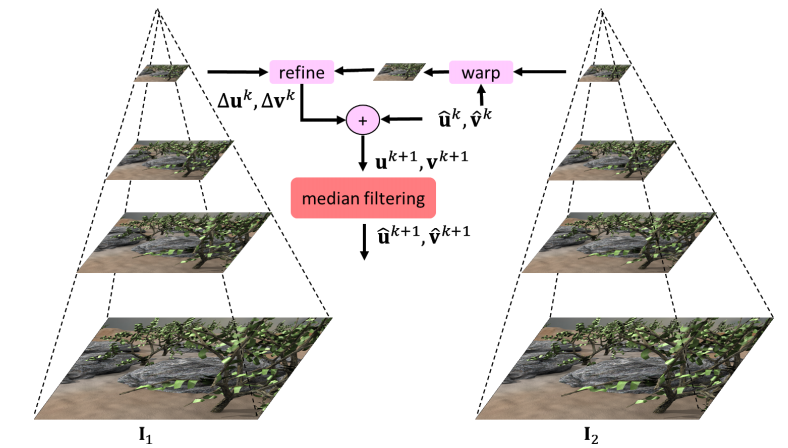
\includegraphics[scale = 0.45]{figures/coarse_to_fine.png}} 
  }
  \caption[coarse_to_fine]{A schematic example of a multi-level coarse-to-fine computation strategy. The top level of image pyramids represent the coarsest level and the bottom level of pyramid corresponds to the original image representation. The computation scheme includes image warping \ref{compensation} and median filtering of intermediate flow results \ref{flow_median}.  Image: \cite{Sun14}}
  \label{fig:coarse_to_fine}
\end{figure*}

Putting the incremental definition of the overall flow field we rewrite the image function $I(x+u^{k+1}, y+v^{k+1}, t+1)$ in the following way:
$$ I(x+u^{k+1}, y+v^{k+1}, t+1) = I(x+u^{k}+du^{k}, y+v^{k}+dv^{k}, t+1) $$
Next, we perform a first-order Taylor expansion around the point $I(x+u^{k+1}, y+v^{k+1}, t+1)$, which gives us:
\begin{eqnarray}
I(x+u^{k}+du^{k}, y+v^{k}+dv^{k}, t+1) &=& I(x+u^{k}, y+v^{k}, t+1) \nonumber \\ &+& I_{x}(x+u^{k}, y+v^{k}, t+1)du^{k} \nonumber \\ &+& I_{y}(x+u^{k}, y+v^{k}, t+1)dv^{k} \nonumber
\end{eqnarray}
Finally we can write the Euler-Lagrange equations:
\begin{eqnarray}
I_{x}(x+u^k, y+v^k, t+1) (& & I_{x}(x+u^{k}, y+v^{k}, t+1)du^{k} \nonumber \\ &+&  I_{y}(x+u^{k}, y+v^{k}, t+1)dv^{k} \nonumber \\ &+& I(x+u^{k}, y+v^{k}, t+1) - I(x,y,t)) \nonumber \\ &-& \alpha \: \textrm{div} (\Psi'(|\nabla (u^{k} + du^{k})|^2 + |\nabla (v^{k} + dv^{k} )|^2) \cdot \nabla (u^{k} + du^{k}) ) = 0 \nonumber
\end{eqnarray}
\begin{eqnarray}
I_{y}(x+u^k, y+v^k, t+1) (& & I_{x}(x+u^{k}, y+v^{k}, t+1)du^{k} \nonumber \\ &+&  I_{y}(x+u^{k}, y+v^{k}, t+1)dv^{k} \nonumber \\ &+& I(x+u^{k}, y+v^{k}, t+1) - I(x,y,t)) \nonumber \\ &-& \alpha \: \textrm{div} (\Psi'(|\nabla (u^{k} + du^{k})|^2 + |\nabla (v^{k} + dv^{k} )|^2) \cdot \nabla (v^{k} + dv^{k}) ) = 0 \nonumber
\end{eqnarray}

This system of equations has to be solved on each computation level $k$ with respect to the motion increments $du^{k}$ and $dv^{k}$. Since we assume that these increments are small the linearization procedure is valid and can be applied. After the flow increments for the current level are computed we find the overall solution as $u^{k+1} = u^{k} + du^{k}, v^{k+1} = v^{k} + dv^{k}$. With such a coarse-to-fine strategy we perform the flow computation step-by-step, so instead of a non-convex optimization we solve a series of convex problems and successively refine the result.
 
In order to implement such a hierarchical approach we have to consider an appropriate implementation to obtain the motion compensated image $I(x+u^k, y+v^k, t+1)$ at a computation level $k$  and the realization of a multi-level strategy (construction of image pyramids).

%----------------- TO CHECK ------------------

%\change{From: \cite{Secrets}. We adaptively determine the number of pyramid levels so that the top level has a width or height of around 20 to 30 pixels.}
%\comment{Give small discussion here}
%\change{From: \cite{Middl}. A limitation of many coarse-to-fine algorithms, however, is the tendency to over-smooth fine structure and to fail to capture small fast-moving objects. Make a reference to Middl paper}


\subsubsection{Motion Compensation}
\label{compensation}

We first discuss the implementation of the motion compensation procedure. The computation of the image function $I(x+u, y+v, t+1)$ and its derivatives $I_x(x+u, y+v, t+1)$, $I_y(x+u, y+v, t+1)$ requires to "apply"  the computed flow field on the initial image, so-called \textit{image warping} \cite{Memin98}.  In this work we follow the approach proposed in \cite{Memin98, Brox04} and perform a \textit{backward registration}. A number of different implementations are possible (see Section \ref{multilevel}). Here we show an example of motion compensation using bilinear interpolation.

We decompose the real-valued computed flow field $u$ and $v$ into two parts: $u = \hat{u}  + \epsilon_u, v = \hat{v}  + \epsilon_v$ where $\hat{u}, \hat{v}$ denote the integer fraction of $u, v$ and $\epsilon_u, \epsilon_v$ denote the subpixel displacement. Then we compute the motion compensated image $I(x+u,y+v,t+1)$ by means of bilinear interpolation using:
\begin{eqnarray*}
[I(x+u,y+v,t+1)]_{i,j,t+1} = & & (1-\epsilon_u)(1 - \epsilon_v) I_{(i+\hat{u}),(j+\hat{v}), t+1} \\
&+& ( \epsilon_u)(1 - \epsilon_v) I_{(i+\hat{u}) + 1,(j+\hat{v}), t+1} \\
&+& (1-\epsilon_u)(\epsilon_v) I_{(i+\hat{u}),(j+\hat{v})+1, t+1}  \\
&+& (\epsilon_u)(\epsilon_v) I_{(i+\hat{u})+1,(j+\hat{v})+1, t+1} 
\end{eqnarray*}
The motion compensation procedure for the image derivatives $I_x(x+u,y+v,t+1)$, $I_y(x+u,y+v,t+1)$ can be performed in the analogous way.

\subsection{Multi-level Computation}
\label{multilevel}

In order to implement a coarse-to-fine strategy we need to specify a transfer function which downscales the original image version to a coarser resolution level and interpolates the obtained results back to the finer computation level. 
On each computation level $k$ the image size is determined via:
$$ N^k_{d} = N^{orig} _{d} \eta^k,$$
where $\eta$ is a warping scale parameter, $N_d$ denotes the image size in the dimension $d \in (x,y)$.

For this purpose a number of approaches can be used such as nearest neighbour averaging, area-based averaging \cite{Bruhn05}, billinear or bicubic interpolation. 
%-------------------------------
%  Not useful
%-------------------------------
%\begin{figure*}[ht]
%  \centerline{
%    \mbox{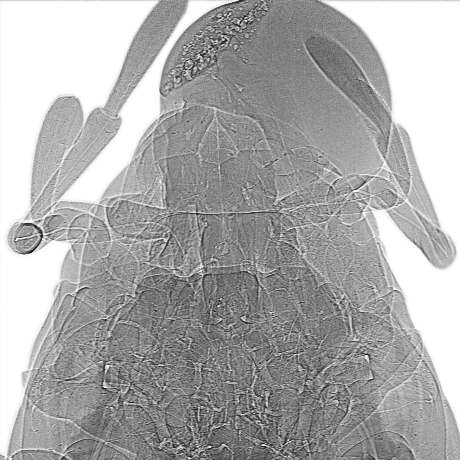
\includegraphics[scale=0.3]{figures/bug_scale1.png}}
%    \mbox{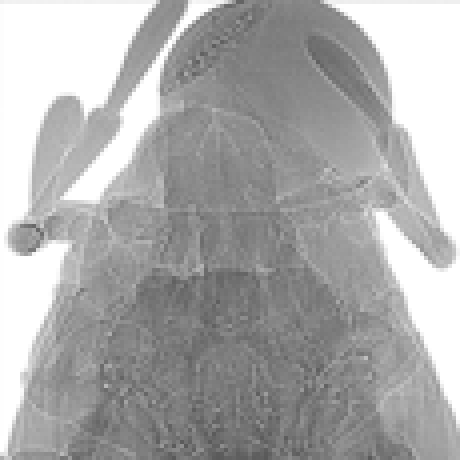
\includegraphics[scale=0.3]{figures/bug_scale4.png}}
%    \mbox{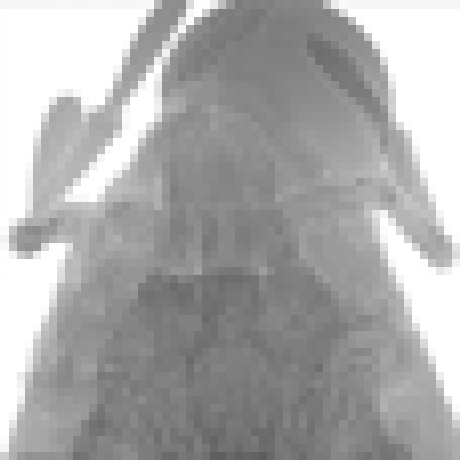
\includegraphics[scale=0.3]{figures/bug_scale8.png}}
%  }
%  \caption[]{Image pyramid constructed using bicubic interpolation on different computation levels. \textbf{Left:} Original level. Original size = (460, 460). \textbf{Center:} Coarse scale = 0.25. Coarse size = (115, 115). \textbf{Right:} Coarse scale = 0.125. Coarse size = (57, 57).}
%  \label{fig:image_pyramid}
%\end{figure*}
In the current work for the construction of image pyramids we use bicubic interpolation using Coons patches \cite{Coons67}. This method gives good results \cite{Sun14, HarmonyFlow}, efficient and easy to implement. For the case of using 3D tomographic data as an input, we employ tricubic interpolation.



\subsection{Intermediate Flow Filtering}
\label{flow_median}

In the work of \cite{Sun10, Sun14} authors reveal a preprocessing step which allows to significantly improve the accuracy and, which  is more important, robustness of optical flow estimation \cite{Wedel09}. It is proposed to apply a median filtering to the intermediate flow result prior to the warping step to the next computation level.

The reason for its surprisingly good results is straightforward. The errors in flow estimation which appear on the coarse image scale are propagated via a warping step to the next level. On this level the incorrect flow serves as an initialization for optical flow estimation.  This results in an accumulation of errors during incremental computation procedure. The median filtering allows to suppress flow errors already on earlier computation levels. With this approach the current optical flow solution is computed via $\textbf{w}^{k+1} = M_p (\textbf{w}^{k} +\textbf{dw}^{k})$, where $M$ is a median filter and $p$ is its mask size. 

In \cite{Sun10, Sun14} it is concluded that optimal size of the median mask is ($5 \times 5$), which outperforms both ($3 \times 3$) and ($7 \times 7$) settings.
In our work we generalize the median filtering approach and use a more adaptive strategy for the flow correction. First, we might observe that on the most coarse computation level, when the image size is the smallest (around 20-50 pixels) median mask of size ($5 \times 5$) may oversmooth the flow result, which can lead to inaccurate flow estimation. To avoid that, we apply less strict filtering on coarse levels using a smaller mask of $3 \times 3$ pixels.

Additionally, in the presence of high amounts of noise or severe artifacts we use a selective filtering using a larger mask ($7 \times 7$ and $9 \times 9$ ). We perform such filtering in homogeneous image regions determined using the same median filtering ($7 \times 7$ or $9 \times 9$) on the original image.  
We present evaluation results in the experimental section \ref{exp_flow_median}.

% \subsection{Anti-aliasing}
% \label{antialiasing}

% In the recent work of \cite{HarmonyFlow} it was shown that high frequency brightness variations in combination with certain amount of displacements can introduce artifacts related to image aliasing.
% The authors proposed to apply a low-pass filtering prior to downsampling for the construction of image pyramids.

% Since X-ray data can potentially contain such high frequency features (for example, morphological structures, tissues, etc) we follow the idea presented in \cite{Sun14} and apply Gaussian filter with a standard deviation $ \frac{1}{\sqrt{2 \eta}} $, where $\eta$ denotes the downsampling factor.


%\subsection{[OPTIONAL] Data Range}
%
%\begin{itemize}
%	\item Discuss the influence of extended data bit range on precision of OF.
%	\item Show on examples: 8-bit and 32-bit floating point \comment{How to make a GT image for floating point?}
%\end{itemize}



%%--------------------------------------------------------
%\section {Performance}
%\label{performance}
%%--------------------------------------------------------
%
%\subsection{Motivation}
%
%\subsection{Advanced Numerical Schemes}
%\label{advanced_numerics}
%
%\subsubsection{Successive-Overrelaxation}
%
%\comment{Write down possible disadvantages. Oversmoothing?}
%
%\subsubsection{Adaptive Interations}
%
%Adapt number of iterations according to current warping level: the less is the size -- the less iteratins we need. Show difference 
%
%\subsubsection{Multigrid Methods}
%
%\comment{What else? Should be added something}
%
%%\section{Input splitting strategies}
%%Including multiprocessors and GRID
%
%\subsection{Efficient Strategies}
%\label{efficient_strategies}
%
%
%\subsubsection{Efficient multi-level strategy}
%\todo{Add more information about efficient implementation of multi-level strategy. \cite{CGF3013}}
%\change{From: \cite{CGF3013} Adaptive multi-scale strategy which tries to isolate image regions where the flow changes slowly. In these regions we replace the computationally expensive energy minimization operation by a simple interpolation. } 
%
%
%\subsubsection{Combining Different Algorithms}
%
%\todo{Give reference to Fusion Flow paper}
%\comment{Add information about combination of efficient and fast implementation with a successive run of high precision OF implementation . From \cite{CGF3013} Show references}
%
%\subsection{Parallelization on  GPU}   
%\label{gpu} 
%
%\todo{Check and include references}
%\change{From: \cite{HarmonyFlow} Following the trend of parallel
%implementations on modern GPUs (Zach et al. 2007;
%Grossauer and Thoman 2008; Sundaram et al. 2010; Werlberger
%et al. 2010) we recently came up with a GPU version
%of our method that can compute flow fields of size 640×480
%pixels in less than one second (Gwosdek et al. 2010).}
%


%--------------------------------------------------------
\section{Summary}
%--------------------------------------------------------

In this section we summarize all models and features which are available in our optical flow framework. In  Table \ref{tab:models_overview} we provide the references to the original papers, where a particular approach  was introduced or discussed, as well as give a reference to the corresponding parts of this work. 
\renewcommand{\arraystretch}{1.2}
\begin{table}[!ht]  \small
  \centering
  \caption{A summary of methods implemented within the optical flow framework presented in this work.}
\begin{tabular}{ |l|l|l|l| } 
%\begin{tabular}{ |c|c|p{7cm}|c| }
\hline
 & Model & References & Section \\ \hline
\multirow{8}{*}{\begin{sideways} Data term \hspace{0pt} \end{sideways}}
 & Brightness constancy 	& \cite{LucasKanade81, HornSchunck81} & \ref{brightness_constancy_assumption}  \\
 & Gradient constancy 	& \cite{Schnorr93, Brox04, Papenberg06} 	& \ref{gradient} \\
 & Higher-order derivatives & \cite{Papenberg06} 							& \ref{high_order_constancy} \\
 & Multiple image features & \cite{Brox04, HarmonyFlow} 				& \ref{assumptions_on_multiple_image_features} \\
 & Combined Local-Global& \cite{Bruhn02, Bruhn05a} 						& \ref{clg} \\
 & Robust Modeling & \cite{Black91, Black96, Sun14, Middl} 			& \ref{robust} \\
 & Joint and Separate Modeling & \cite{Bruhn05b, HarmonyFlow}		& \ref{joint_and_separate} \\
 & Data Normalization & \cite{Lai98, HarmonyFlow} 						& \ref{normalization} \\ 
\hline
\multirow{5}{*}{\begin{sideways}Smoothness \hspace{3pt}\end{sideways}} 
 & Homogeneous & \cite{HornSchunck81}   &  \ref{homogeneous_smoothness} \\
 & Image-driven & \cite{Schnorr93, Alvarez99, Weickert00b}   & \ref{image_driven}  \\
 & Flow-driven &  \cite{Schnorr94, Brox04, Papenberg06}   & \ref{flow_driven}  \\
 & Spatial-temporal & \cite{Nagel90, Weickert2001b}    & \ref{spatial_temporal} \\
 & Adaptive smoothness & \cite{HarmonyFlow}   & \ref{adaptive_smoothness} \\ 
\hline
\multirow{6}{*}{\begin{sideways}Optimisation\end{sideways}} 
 & Coarse-to-fine strategy & \cite{Black96, Memin98, Brox04}   & \ref{coarse_strategy} \\
 & Flow median filtering & \cite{Wedel09, Sun14}   & \ref{flow_median} \\
 %& Anti-aliasing & \cite{HarmonyFlow, Sun14}   & \ref{antialiasing} \\
 & Multiple results fusion & \cite{Lempitsky08}   & \ref{assumptions_on_multiple_image_features} \\
 & User-driven landmarks & \cite{Fischer03}     & \ref{landmarks} \\
 & Confidence measures & \cite{Fua93, Brown03, Bruhn06, Xu10}   & \ref{confidence_measures} \\
 & Parameters optimization & \cite{HarmonyFlow}   & \ref{parameters_optimization} \\ 
\hline
\multirow{3}{*}{\begin{sideways} Compute \hspace{7pt}  \end{sideways}} 
 & 2D images & ---    &  \ref{data_constancy_assumptions}, \ref{smoothness_assumptions} \\
 & 3D images & ---    &  \ref{extension_3d} \\
 & Efficient schemes & \cite{Brox04, BruhnThesis, CGF3013}    &  \ref{advanced_numerics}  \\
 & GPU computation & ---   & \ref{gpu} \\
\hline
\end{tabular}
\label{tab:models_overview}
\end{table}


%******************************************************************
%******************************************************************
\chapter {Data Analysis Framework}
\label{data_preprocessing}
%******************************************************************
%******************************************************************

This chapter is dedicated to analysis of time-resolved X-ray data. It divides into two extensive sections: data enhancement (Section \ref{data_processing}) and further analysis of the computed optical flow results (Section \ref{data_analysis}).
 
In Section \ref{data_processing} we start the discussion of data pre-processing (or filtering) to correct image defects. This step always precedes any further data treatment and optical flow computation. We consider three topics which are of key importance: image noise filtering, brightness corrections and contrast adjustment.     

In Section \ref{data_analysis} we give a list of data analysis routines which we employ in the application section of the current work. These routines, together with a variety of optical flow methods constitute our framework for time-resolved data analysis. We distinguish five individual \textit{tasks}: analysis of the computed motion field; motion-based segmentation; detection of temporal changes which are not attributed to the motion itself; automated tracking and image registration/alignment.

%In Section \ref{visualization} we present and briefly discuss data visualization methods used in the scope of this work to depict the result of optical flow computation (i.e. the displacement field) and results of the further motion analysis.       
 

%--------------------------------------------------------
\section{Data Preprocessing}
\label{data_processing}
%--------------------------------------------------------

In this section we present a first step in our data treatment pipeline, namely data preprocessing. The purpose of this step is to correct various image defects that might be present due to  non-optimal experimental conditions, physical properties of the process, imprecise detector system, or  artificial errors introduced by an image reconstruction procedure. Such image defects might deteriorate the result of data analysis and thus should be corrected before any further optical flow computation or analysis steps are undertaken.

We assume that data which is provided for the image processing already represents the best possible quality which can be achieved by the data acquisition process. Otherwise, the experimental conditions should be readjusted and optimized. However, this is not always possible and frequently the image acquisition system is employed to its technical limits. 

As an example, image noise affects the ability to detect small feature details, especially for the low contrast data - when brightness level differs only slightly for separate image features. To increase signal-to-noise ratio and, thus, to improve data quality, it is necessary to increase the number of detected photons. This can be done by increasing the beam intensity, increasing the exposure time or acquiring and averaging several image frames. All of this, however, will lead to a higher dose deposition, which can affect the viability of the specimen in the case of biological applications. Another option is to increase the pixel size by combining several neighbor pixels, which will allow to detect more photons, resulting in a higher signal-to-noise ratio. But, in this case, the improvement in signal-to-noise ratio is obtained at the expense of poorer spatial resolution. This illustrates a fundamental trade-off between image quality and dose deposition. Moreover, there is also a trade-off between individual parameters of image quality, i.e. spatial resolution, features contrast and noise. Furthermore, the optimization of experimental setup could be time consuming and, given the limited time for experiments on a synchrotron, dealing with image data as a post-processing step could be more practical. That is why it is reasonable to sacrifices the image quality for the ability to capture physical characteristics of dynamical process, and then utilize data processing as a correction step. 

It is important to emphasize, that by the term \textit{data preprocessing} we assume both data restoration (correction) and data enhancement. However, both procedures are not the same and serve different purposes. Unlike data enhancement, which is a subjective routine and aimed on improving visual appearance of certain image details or features, image restoration is based on mathematically justified image correction. There might be cases when the same image processing procedure serves both purposes. For example, correcting image brightness variations could improve visual analysis of image sequences, since image flickering could be distracting and obscure important changes. On the other hand, it could also correct pixel data for the use of certain optical flow models (e.g. grey value constancy assumption).



 


\subsection{Noise Filtering}
\label{noise_filtering}

\textit{Image noise} is the unwanted fluctuations of the pixel brightness in an image. This results in a degradation of image quality and deteriorates data analysis.  The noise which is generated within an imaging system is usually a combination of a number of independent noise
sources. In general, it is not possible to identify, and thus to filter individual noise contributions separately. To quantify image variations due to the noise, a scene in which the resulting image is expected to have a uniform brightness might be used. Then, a noise content of the image (noise power $P_n$) is given by the variance, i.e. the square of the standard deviation, of the pixel grey values in local image region. To estimate the noise influence one should compare it with the average amount of intensity in the same region (signal power $P_s$).  The \textit{signal-to-noise} ratio (SNR) is the ratio of the intensity of the signal (pixel brightness) to the noise power $SNR = \frac{P_s}{P_n}$. However, in cases when noise properties cannot be described as random or having \textit{normal} statistical distribution, it is more difficult to estimate the amount of noise. 

In the following sections we shortly describe a number of \textit{noise models} which are the most relevant for the processing of X-ray images and optical flow analysis. Then we provide correction techniques (noise filters) which allow us to reduce the amount of noise and to recover useful information. This, in turn, will improve the results of optical flow computation.   




\subsubsection{Noise Models}
\label{noise_models}

The common sources of noise in images taken with X-ray imaging systems are photon noise, which originates due to the discrete nature of X-ray radiation (and electromagnetic radiation in general) and interaction of X-ray with matter, and electronic noise from the digital detector systems. Additionally, the process of digitization also adds noise (quantization noise), but we assume that this type of noise does not contribute much to the overall noise level.
\\
\\
\textbf{Gaussian noise}
\\
A popular noise model which is considered in various fields of Signal Processing and Computer Vision is \textit{Gaussian noise}. It has a probability density function (or normalized histogram), which is given by:
$$G(x,\mu, \sigma)= \frac{1}{\sigma \sqrt{2 \pi}} e^{-\frac{(x-\mu)^2}{2\sigma^2}}, $$
where $x$ is the pixel brightness, $\mu$ is the mean brightness value and $\sigma$ is its standard deviation.
This model is a very convenient from the mathematical point of view and simulates many real world random (stochastic) processes. That is why it is widely used in image processing to contaminate images with noise.  However, this model does not adequately represent physical properties of image acquisition process in most medical systems, including X-ray imaging, where an image has a spatial and temporal randomness characterized by Poisson statistics. 

In the current work we decide to keep this noise model for the sake of having a systematic experimental approach and direct comparability with the literature on optical flow. We start all the experiment on noisy images with this simple model and then proceed with the more suitable ones such as photon and impulse noise models. 
\\
\\
\textbf{Photon noise}
\\
\textit{Photon noise} (also known as quantum noise or shot noise) arises from the statistical properties of electromagnetic radiation - an imaging sensor receives within a time interval of $\Delta t$ (exposure time) on average $N$ electrons by absorption of photons. The average rate of received photons per unit time $\lambda$ is given by $\lambda = \frac{N}{\Delta t}.$  During each exposure a different number of photons are registered by the detector element. A random process in which an average $\lambda \Delta t$ events are counted is described by a Poisson distribution $P(\lambda \Delta t)$:
$$ P(\lambda \Delta t) = \frac{(\lambda \Delta t)^n}{!n}  e^{- \lambda \Delta t}, n \geq 0,$$
with the mean and variance: $\mu = \lambda \Delta t $ and $\sigma^2 = \lambda \Delta t$ respectively.  An important property of a random process according to Poisson distribution is that it is not independent of a signal and is not additive. Additionally, the signal-to-noise ratio increases as an average brightness level gets larger, which means that the more x-ray photons are detected, the higher the signal-to-noise is and the less noise is contained in the image data. The
photon noise is a fundamental and unavoidable source of noise in medical imaging. For an efficient and optimized imaging system it is the dominant source of random fluctuation in image data \cite{Dougherty09}.

An important contribution of our work is that in addition to a classical Gaussian noise model we include an extensive discussion of performance of optical flow methods on a physically justified noise model such as photon noise.
\\
\\
\textbf{Spike noise}
\\
Another type of noise which could be useful to consider for our class of applications is so-called \textit{impulse noise} (also salt-and-pepper or \textit{Spike} noise). This type of noise is usually caused be the errors in data transmission or damaged sensor elements  of the digital detector system ("dead" or saturated pixels).  The strength of the corruption by impulse noise is usually of much more influence compared to other types of noise, since such type of noise is recorded as an extreme values, so they are equal or close to the maximum and minimum values of dynamic range of an image.
This type of noise is usually quantified by the percentage of pixels which are corrupted.

Despite the fact, that sometimes it is possible to correct such corrupted pixels using the dark field correction (which will be described later in Section \ref{flat_field_correction}), we choose to include this type of noise in our experiments on noise. We consider this type of noise as very helpful to evaluate  the performance of optical flow methods and data correction techniques with respect to data outliers.
   


\subsubsection{Noise Filters}
\label{noise_filters}
         
In the previous section we introduced several noise models which we will use for our experiments on noisy data (Sections \ref{exp_noise} and \ref{experiment_noise_reduction}). Here we present methods to restore image details from the noisy images, with the aim to possibly improve results of optical flow computation. There is a tremendous amount of literature on image denoising methods. For this work we limit our experiments only on those methods which are widely available, easy to implement and are well understood from the mathematical point of view. Here we do not aim to fully cover this topic. For in-depth information on denoising methods the reader is referred to the extensive literature. To enhance image data with respect to noise we consider four filters: Gaussian filter, bilateral filter, median filter, anisotropic diffusion filter.

An important assumption for any denoising method is that the pixel size (resolution) is much smaller then the important details which we aim to recover.  
\\ 
\\
\textbf{Gaussian Filter}

A commonly used approach to filter noise is a \textit{Gaussian smoothing}. 
It can be implemented as a convolution of the image with the Gaussian function. This  filter reduces noise  from the image, however, it also blurs image edges and reduces image contrast.   It can introduce other artifacts such as merging of nearby structures. Moreover, the data outliers are not completely filtered, but only averaged in a local neighborhood, which means that the corrupted pixel data could be spatially extended. Note, that Gaussian smoothing corresponds to the linear isotropic diffusion process. The implementation of Gaussian low-pass filtering is done via computing a weighted average of pixel values in the neighborhood, with the
weights decreasing with the distance from the neighborhood center.
\\ 
\\
\textbf{Bilateral Filter}

\textit{Bilateral filtering} removes the noise while preserving image
edge information, which is done by a weighted average of intensity values from nearby pixels.
An important property of the bilateral filter, is that the weights depend on both geometrical closeness of the pixels and their photometric differences (e.g. grey values) \cite{Tomasi98}.

The filtering procedure can be expressed in the following way:
$$I_{bilateral}(\textbf{x}) = \frac{1}{W_p} \sum_{\textbf{x}_i \in \Omega} I(\textbf{x}_i) f_r(|I(\textbf{x}_i) - I(\textbf{x})|) g_r(|\textbf{x}_i - \textbf{x}|),$$
where the normalization factor is:
$$W_p = \sum_{\textbf{x}_i \in \Omega} f_r(|I(\textbf{x}_i) - I(\textbf{x})|) g_r(|\textbf{x}_i - \textbf{x}|),$$
where $I$ is the original image, $x$ is the coordinate of the current pixel being processed; $\Omega$ is the spatial window mask centered at location $x$; $f_r$ is the range kernel to filter differences in pixel brightness; $g_s$ is the spatial kernel to filter differences in geometrical distances. 

Among the advantages of the bilateral filter are simple implementation and non-iterative nature of the algorithm.
\\
\\
\textbf{Rank Filters}

A drawback of smoothing or averaging filters is that they produce undesirable blurring on object boundaries, which are represented by image edges. A possible solution to this problem is to discriminate pixel values by ranking them in a local neighborhood. A common choice is a \textit{median filter} which selects the median value in the ordered list of grey values and uses this value as a new result for the central pixel.  
Median filter provides excellent performance for certain types of noise, especially impulse noise, which was discussed in the previous section. If a pixel contains an extreme brightness value ("dead" or saturated pixel), it is substituted by an acceptable value from a local neighborhood.
The important property of the median filtering is that is an \textit{edge-preserving filter}. However, for very large neighborhood sizes small image details could be completely eliminated.  

To implement a median filtering one may choose between different  sizes and shapes of the neighborhood. Several mask patterns are possible: a 4-nearest neighbor cross, a ($3 \times 3 $) square,  a ($5 \times 5 $) circular, etc. This different neighborhood patters are shown in Figure \ref{fig:median_mask}. Typically, a square mask is easier to implement, however, as the mask size increases the use of a pattern which approximates a circular region is important to produce more isotropic filtering \cite{Russ11}. For implementation of median filtering in the current work we opt to use a circular median filtering mask. 


\begin{figure*}[ht]
  \centerline{
    \mbox{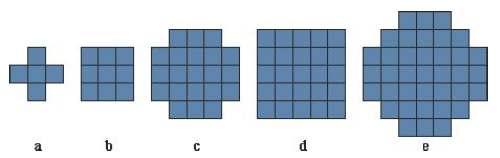
\includegraphics[scale=0.55]{figures/median_mask.png}}
  }
  \caption[]{Shapes of 2D neighborhood mask for median filtering. \textbf{(a)} 4-nearest neighbor cross. \textbf{(b)} a ($3 \times 3 $) square. \textbf{(c)} ($5 \times 5 $) circular. \textbf{(d)} ($5 \times 5 $) square. \textbf{(e)} ($7 \times 7 $) circular. Image: \cite{Russ11}.}
  \label{fig:median_mask}
\end{figure*}

Another useful approach is to consider a more sophisticated ranking of neighborhood information. This step is driven by the fact, that median filter removes small details which are twice smaller then the size of the median mask and also removes sharp corner details. A special case of corner-reserving median filter, is a \textit{hybrid median filter} \cite{Nieminen87, Russ11}. This filter ranks all the pixels in different sets. In the first group there are 4 nearest neighbours forming a "+" sign and the second group are pixels which are located in diagonal locations with respect to the central pixel (forming a "x" sign). Then, median values from these two sets are compared with the central pixel. The idea is sketched in  Figure \ref{fig:hybrid_median_filter}.
\begin{figure*}[ht]
  \centerline{
    \mbox{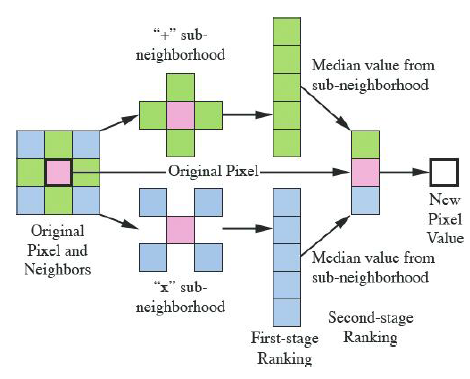
\includegraphics[scale=0.65]{figures/hybrid_median_filter.png}}
  }
  \caption[]{A sketch of hybrid median filter, which preserve corners and small coherent structures. Image: \cite{Russ11}}
  \label{fig:hybrid_median_filter}
\end{figure*}
\\
\\
\textbf{Anisotropic Diffusion}

\textit{Anisotropic diffusion} (also known as Perona - Malik diffusion \cite{Perona90}) is a method which aims to reduce image noise without removing image edges representing an important features. Additionally, such types of filters can posses even edge-enhancing properties \cite{Weickert98}. The smoothing is done by means of a diffusion process in which the strength of the diffusion is controlled by derivatives of the image brightness values.
Anisotropic diffusion is define as:
$$ \frac{\partial I}{\partial t} = \text{div} ( c(x,y,t) \nabla I),$$
where $I(x,y,t)$ is an image in a domain $ \Omega_{2} \subset \mathbb{R}^2$, $\nabla$ denotes gradient operator, div() is a divergence operator, $c(x,y,t)$ function controls the rate of diffusion depending on image data at pixel location $(x,y)$.
In a seminal paper of Perona and Malik the diffusivity $c(x,y,t)$ are:
$$c(|\nabla I|) = e^{-(|\nabla I| / \epsilon)}$$
or
$$c(|\nabla I|) = \frac{1}{1 + (\frac{|\nabla I|}{\epsilon})}$$
where $|\nabla I|$ is a magnitude of the image gradients and $\epsilon$ is constant which is choose experimentally or depending on a noise scale.

Anisotroipic diffusion is a flexible and highly adjustable filter. With different parameters one my obtain a very distinctive filtering results. However, what might be an advantage to produce better results, also can be a drawback, since it is not easy to optimize numerous parameters to get the best possible result. Additionally, the implementation is not trivial and the filter is computationally demanding (being an iterative method). 

Carefully weighting all pros and cons we use this filter for our quantitative comparison of denosing filters, since anisotropic diffusion is a powerful and flexible method, with many degrees of freedom. 

We use an implementation based on the paper of \cite{Tschumperle05}. A freely available implementation can be access via a web link: \\
\url{http://rsb.info.nih.gov/ij/plugins/anisotropic-diffusion-2d.html}.  

%-------------------------------
% Temporally excluded
%-------------------------------
%\\
%\\
%\textbf{Non-Local Means}
%\todo{Include or exclude from thesis}



\newcommand{\imageSize}{0.65}

\begin{figure*}[!ht]
  \centerline{
    \mbox{\includegraphicslabeledw[scale= \imageSize]{figures/noise_rub1_original_crop.png}{a}}
    \mbox{\includegraphicslabeledw[scale= \imageSize]{figures/noise_rub1_sigma_2p0_crop.png}{b}}
  }
  \vspace{3pt}
  \centerline{
    \mbox{\includegraphicslabeledw[scale= \imageSize]{figures/noise_gauss_2p0_crop.png}{c}}
    \mbox{\includegraphicslabeledw[scale= \imageSize]{figures/noise_median_3p0_crop.png}{d}}
  }
  \vspace{3pt}
  \centerline{
    \mbox{\includegraphicslabeledw[scale= \imageSize]{figures/noise_bilateral-5p0-70_crop.png}{e}}
    \mbox{\includegraphicslabeledw[scale= \imageSize]{figures/noise_anisotropic-iter20_a1_0p5_a2_0p9_dt_20_edge_15_crop.png}{f}}
  }
  \caption[Noise filterst]{Performance of noise filters on \rub dataset with Gaussian noise with $n_{\sigma}$=10. \textbf{(a)} First frame of original image. \textbf{(b)} With Gaussian noise with $n_{\sigma}$=10 added.  \textbf{(c)} Gaussian smoothing filter. \textbf{(d)} Median filter. \textbf{(e)} Bilateral filter. \textbf{(f)} Anisotropic diffusion filter.}
  \label{fig:noise_filters}
\end{figure*}
\vspace{7pt}

\noindent Comparison of different noise filtering methods is presented in Figure \ref{fig:noise_filters}.

                 
\subsection{Brightness Correction}
\label{brightness_correction}


The most commonly used assumption in image analysis to identify or compare pixel values is that the region representing the same object or feature should have the brightness value. However, in practice for real-world imaging scenarios such strict conditions could not always be fulfilled. 

For X-ray imaging the constancy and uniformity of the background brightness distribution can be affected because of various reasons, such as non-uniform beam profile due to spatio-temporal fluctuations of a light source, etc.  
Usually such effects can be corrected by recording a background image (without an object in the field of view) and then removing non-constant brightness variation (see Section \ref{flat_field_correction}). Depending on the image content, this can be implemented as a subtraction or division operation with a background and the image with an object. However, this procedure is not always feasible, especially for \textit{in-situ} or \textit{in-vivo} experiments, when one acquires a continuous sequence of images and brightness variations occur during the recording time. For this case we propose a proper brightness correction procedure. Here we describe the most popular methods to achieve this and later evaluate how different correction procedures influence the accuracy of optical flow estimation (see Section \ref{experiment_nonuniform_brightness}).          


\subsubsection{Illumination Models}
\label{illumination_models}

As we outlined previously, background brightness distribution can be non-constant over time or non-uniform spatially for a sequence of X-ray images. This property of X-ray data is of crucial importance for the choice of appropriate data constancy assumptions for the design of optical flow models (see Section \ref{data_constancy_assumptions}). In the literature on optical flow methods this problem is referred to as "changing illumination conditions". 

To correctly model optical flow assumptions it is important to consider realistic illumination scenarios. Two important models in the literature on the optical flow are: \textit{additive} illumination and \textit{multiplicative} illumination \cite{Weijer04, Mileva07}. Additionally, one may distinguish between \textit{global} and spatially \textit{local} changes.
In Section \ref{data_constancy_assumptions} on the available data terms  we already discussed that the gradient constancy assumption is invariant under global additive illumination changes, however it is not suited for the case if there is also a multiplicative part.

It is important to note, that increasing an exposure time while recording an X-ray image corresponds to global multiplicative brightness changes. Thus, to apply optical flow methods, an appropriate choice of the data term which is robust under this type of brightness changes is an crucial aspect. This will be discussed in the experimental section \ref{exp_data_terms_brighntness}.

Typically, to tackle with varying brightness conditions optical flow methods make use of different photometric invariants derived from color models \cite{Mileva07, HarmonyFlow}. Such transformations are invariant under general illumination changes.  
However, since color information is not available for X-ray images we are enforced to search for another reliable solutions, which we present in the following sections. 

        

        
\subsubsection{Flat-field Correction}
\label{flat_field_correction}

The simplest approach to correct background non-uniformities is to perform so-called \textit{flat-field correction}. In this case a "flat" image, without an object in the field of view is recorded. Then this image is used to eliminate the brightness pattern from the image with a specimen. In a general form the flat-field correction can be computed as:
$$I_{filt} = \frac{I_{raw} -  I_{dark} }{I_{flat} - I_{dark}},$$
where $I_{raw}$ is a recorded raw image, which has to be corrected, $I_{flat}$ is a flat-field image and $I_{dark}$ is a dark-field image. The dark-field image is an image captured with no illumination. In other words, it is an image of the sensor noise. An average of several dark-field frames provides a possibility to correct for the fixed-pattern noise, including dark ("dead") and saturated ("hot") pixels. 
For the case of X-ray data, since the recorded images represent the absorption of a sample according to the Beer's law (for the case when absorption is dominating the image contrast) we may also perform a logarithm transformation to recover the physical thickness of structures:
$$I_{filt} = \frac{\text{log}(I_{raw} -  I_{dark}) }{\text{log}(I_{flat} - I_{dark})}$$

However, as we mentioned before, a flat-field correction is not always possible for \textit{in-situ} or \textit{in-vivo} experiments.      

\subsubsection{Fitting Background}

One approach to eliminate uneven background from the recorded image, without a flat-field image available is to measure an overall brightness in different parts of the image and then interpolate the result. Then the obtained brightness pattern might be used for image correction. A good choice for the interpolation function is a polynomial interpolation, which gives good results for relatively gradual brightness variations. Another choice is to perform least-squares fitting of sample points distributed over the image domain. The distribution of sample points could be automated (for example using a grid or object detection) or manual.  

\subsubsection{Image Leveling}
\label{image_leveling}

In the case when the background changes more irregularly, so the fitting of a simple function cannot be performed, a different approach might be useful. For this method one assumes that the image features have smaller size then the scale of brightness variations.
The background image is estimated by applying an averaging or ranking filter with a large spatial mask. Than, this background image is subtracted from the original image frame to remove brightness variations.

In the current work we employ two types of filters, namely Gaussian smoothing filter and median filter (See Section \ref{noise_filters}). Important parameters for such a filter are the shape and the size of a spatial mask.  One should note that brightness variations can be one-dimensional (e.g. horizontal stripes patters), in this case the filter can be implemented as a 1D stencil. Figure \ref{fig:image_leveling} shows the application of image leveling methods to correct uneven brightness patterns.

\begin{figure*}[ht]
  \centerline{
    \mbox{\includegraphicslabeledw[scale= 0.38]{figures/contrast_adjust_orig.png}{a}}
    \hspace{3pt}
    \mbox{\includegraphicslabeledw[scale= 0.38]{figures/contrast_adjust_corr.png}{b}}
  }
  \caption[Noise filterst]{Non-uniform background correction using image leveling with the Gaussian smoothing filter with a spatial mask $\sigma=15$. \textbf{(a)} Original image. \textbf{(b)} Corrected image. }
  \label{fig:image_leveling}
\end{figure*}




\subsubsection{Log Transform}

Another approach to deal with local brightness variations (including additive and multiplicative intensity changes) is to use a so-called log-derivatives \cite{Mileva07}.
In this case the original image grey values are transformed into a logarithmic scale, then gradients of these log-derivatives are considered as constancy assumptions for the computation of optical flow. Such transformation is more robust under multiplicative intensity changes.

We evaluate this approach in the experimental Section \ref{exp_data_terms_brighntness}, where we check the performance of different data terms for changing brightness conditions. 




\subsection{Contrast Adjustment}
\label{contrast_adjustment}

The range of brightness values represented on the image is known as the \textit{dynamic range}. It can be measured as a difference between maximum and minimum values. Ideally, the dynamic range obtained by the interaction of the radiation with the sample - for the case of X-ray imaging - should coincide with the available  dynamic range of the detector system. In a case if it is wider than the one of the detector, the image histogram is cutted. The brightness values which fall inside this cutted regions are inevitably lost. Additionally, extreme pixel values which corrupt the range of histogram can be caused by data outliers, such as "dead" or "hot pixels" and can be corrected as a preprocessing step to improve the visibility of image details.

An image property which is related to the dynamic range is a \textit{contrast}. In the case when the dynamic range of an image covers all brightness values produced by the imaging system (including interaction of X-rays with a sample), the image exhibits high contrast. On contrary, when dynamic range is low (only a narrow range of similar grey values present in the image), the image has a low contrast. 
It is important to note, that the dynamic range and image contrast are related, but not identical concepts. For instance, images with bimodal histogram (peaks on the lower and upper parts of the histogram) exhibit higher contrast than images with smooth, even histogram.  For the ideal imaging session one is interested to both cover the full dynamic range of the image and provide maximum feature contrast.    

Since for optical flow methods the pixel grey values are the source of information to solve a correspondence problem, one may try to correct the image contrast not only to enhance the visibility of image details, but also to improve results of optical flow computation. In this section we present a number of techniques to achieve that and in Section \ref{experiment_local_contrast} we evaluate the influence of these methods on the accuracy of optical flow.    



\subsubsection{Contrast Estimation}
\label{contrast_estimation}

In Section \ref{noise_filtering} we discussed an important characteristic of the image, which is a signal-to-noise-ratio (SNR). Here we emphasize that for the analysis of X-ray images (and medical image in general) a concept which is even more important is a \textit{contrast-to-noise ratio} (CNR):
$$C = \frac{|S_1 - S_2|}{\sigma},$$
where $S_1, S_2$ are the brightness of structures in the region of interest and $\sigma$ is the standard deviation of image noise.  
For medical imaging applications the goal is to distinguish between different structures or between an object and a background. For this case the contrast-to-noise ratio is more descriptive and useful measure, since it relates both image noise and image contrast.  


\subsubsection{Contrast Enhancement}
\label{contrast_enhancement}

A frequent situation, especially for X-ray imaging with low exposure conditions, is when the images do not have the brightness range that covers the full dynamic range available for a detector system. On Figure \ref{fig:histogram_stretch} brightness values on the light and dark ends of the histogram are not used.
Expanding the brightness value to cover the full dynamic range may improve the visibility of local image features. This can be implemented with the linear brightness values mapping \cite{Gonzalez08}. This operation is often called the \textit{histogram stretching}. The result of this transformation is shown in Figure \ref{fig:histogram_stretch}b.

\begin{figure*}[ht]
  \centerline{
        \mbox{\includegraphicslabeledw[scale= 0.27]{figures/egg1.png}{a}}
        \mbox{\includegraphicslabeledw[scale= 0.27]{figures/egg2.png}{b}}
  }
  \vspace{3pt}
    \centerline{
    	\mbox{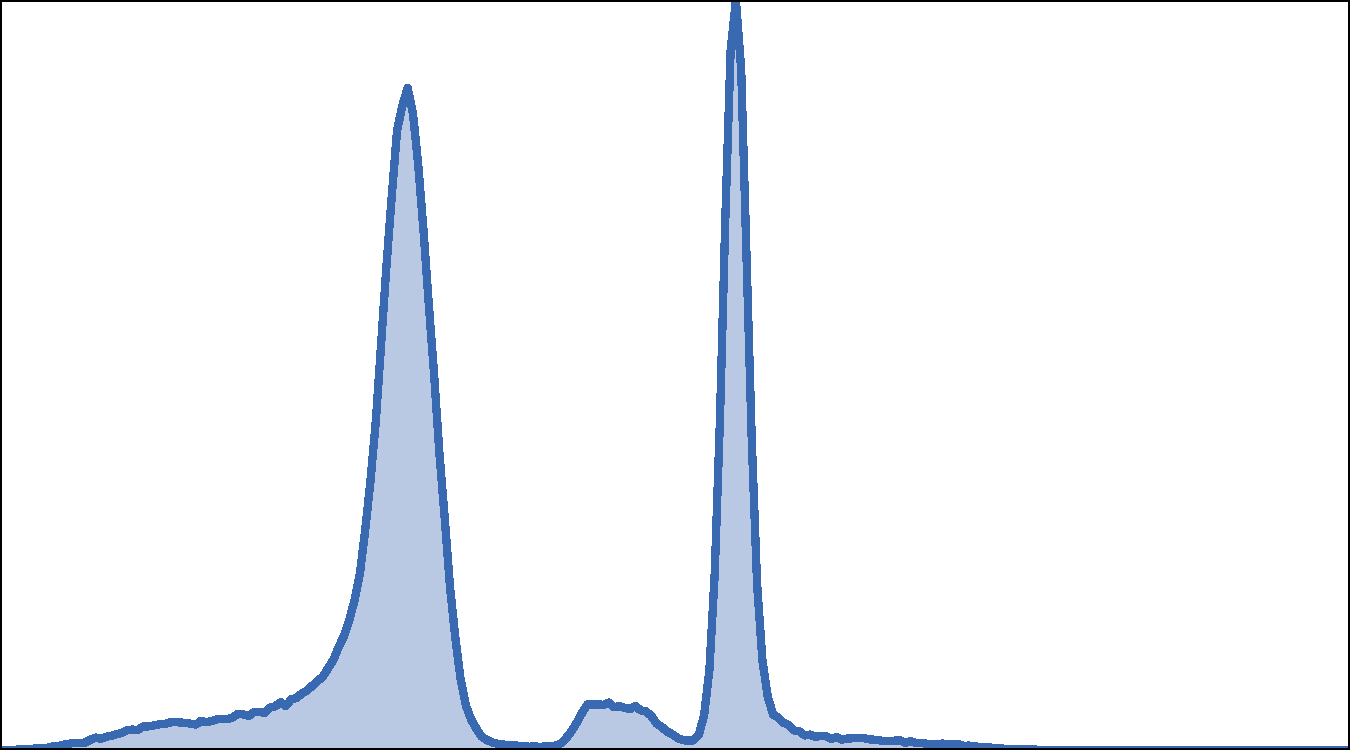
\includegraphics[scale= 0.29]{figures/egg1_hist.pdf}}
    	\mbox{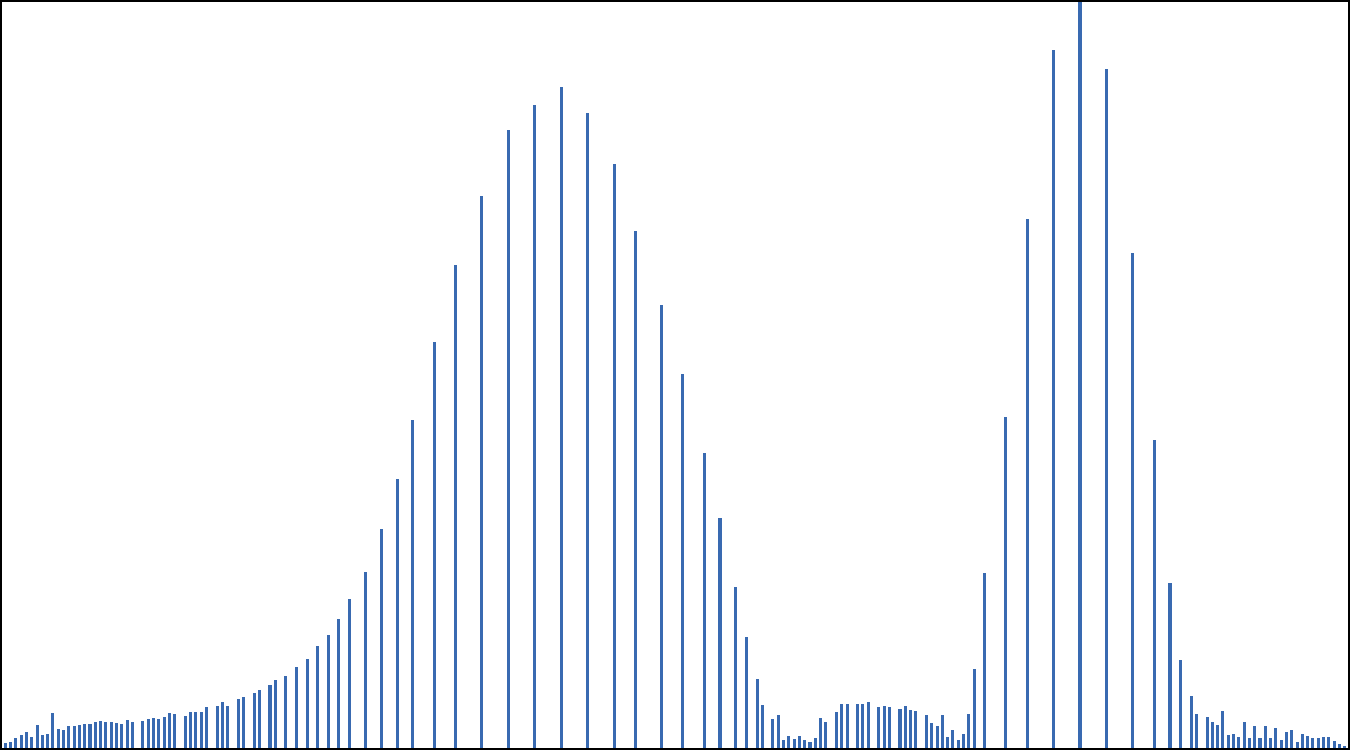
\includegraphics[scale= 0.29]{figures/egg2_hist.pdf}}
    }

  \caption[]{Example of a histogram stretching to improve the visibility of local image features. \textbf{(a)} Original radiograph with poor contrast. \textbf{(b)} Radiograph corrected using histogram stretching.}
  \label{fig:histogram_stretch}
\end{figure*}

In some cases the majority of pixel values occupy a narrow range of a histogram, but a few number of outliers represent extreme values (e.g. hot and dead pixels). In this case the histogram stretching cannot be performed, since the whole histogram range is used. This results in an ineffective use of dynamical range. One way to solve this, is to filter these outliers, e.g. using median filtering. However, this procedure also affects the pixel values in the correct range of brightness range. Alternatively, it is possible to dismiss a certain percentage of pixels on the histogram ends. As a result, these pixels will be saturated with minimum and maximum values, but the rest of histogram range will be used effectively. 

Note, that the aforementioned procedure is global and linear. To improve local visibility of image features, one may perform nonlinear, \textit{local contrast enhancement} \cite{Pizer87}. This technique perform brightness stretching based on a histogram of a local image region.    



%\subsection{[OPTIONAL] Image Decomposition}
%
%\comment{Find further information}

%\subsubsection{OPTIONAL: Edge Enhancement}

%\comment{Check!}


%--------------------------------------------------------
\section{Analysis Based on Optical Flow}
\label{data_analysis}
%--------------------------------------------------------



This section is devoted to an overview of data analysis methods, which can be applied after the optical flow results are computed. By further analysis of the obtained motion field one can extract a vast amount of quantitative information about dynamical processes. Although, several techniques can be closely related, in our \textit{data analysis framework} we identify four separate topics:
\begin{itemize}
	\item Motion / flow analysis 
	\item Motion-based segmentation
	\item Object tracking
	\item Image registration and alignment
	
\end{itemize}
In the following sections we describe in details each of these analysis methods.
   

%--------------------------------------------------------
\subsection{Motion Analysis}
\label{motion_analysis}
%--------------------------------------------------------
            
In this section we present a common techniques to analyze the motion field after the optical flow is computed.  The aim of these methods is to provide quantitative information about dynamical process. 
All of the presented methods are available in our data analysis framework. 

We define a \textit{vector field}  as a map $\textbf{F}: \textbf{R}^n \mapsto \textbf{R}^n $ that assigns each coordinate $\textbf{x}$ a vector $\textbf{F}(\textbf{x})$. 
A vector $\textbf{F}$ in an $n$-dimensional Euclidean space can be defined as an ordered list of $n$ real numbers  $\textbf{F} = \lbrace x_1, x_2, \ldots, x_n \rbrace$.
 
            
\subsubsection{Magnitude}
\label{magnitude}

An important property of a vector is its \textit{magnitude} or length (also referred as velocity). It is commonly defined as a Euclidean norm:
$$| \textbf{F} | = \sqrt{x_1^2 + x_2^2 + \cdots + x_n^2 } $$

Magnitude of the vector field is a useful measure to quantitatively describe physical characteristics of the dynamical process, distinguish between different moving object and analyze the velocity changes over time. 
To compute the magnitude of the flow field one might be interested to distinguish 4 scales:
\begin{itemize}
  \item Magnitude of an individual pixel at the location $\textbf{x}$
  \item Average magnitude within a particular object $O$
  \item Average magnitude inside a certain region of interest (ROI)
  \item Average magnitude for the entire image frame $I(\textbf{x})$
\end{itemize}
    

\subsubsection{Divergence}
\label{divergence}

\textit{Divergence} is a vector operator that measures as a single scalar value to which extent a vector field behaves as a sink or source at a given point. It can be defined for a continuously differentiable vector field $\textbf{F}=(F_x,F_y,F_z)$ as follows:
$$\text{div} \, \textbf{F} = \nabla \cdot \textbf{F} = \frac{\partial F_x}{\partial x} + \frac{\partial F_y}{\partial y} + \frac{\partial F_z}{\partial z} $$


\begin{figure*}[ht]
  \centerline{
    \mbox{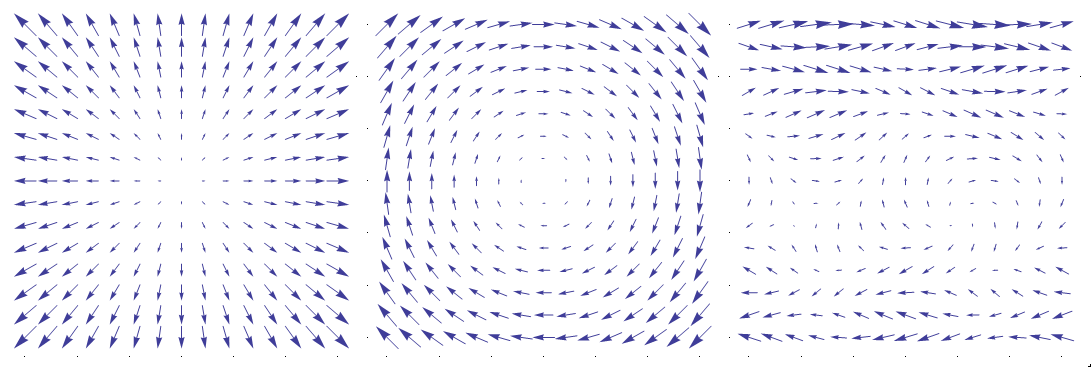
\includegraphics[scale= 0.4]{figures/vector_fields.png}}
  }

  \caption[Noise filterst]{Example of different types of vector fields.  \textbf{Left:} Divergent vector field. \textbf{Middle:} Rotational motion field. \textbf{Right:} Turbulent flow field with a significant amount of flow discontinuities.}
  \label{fig:vector_fields}
\end{figure*}

Divergence is a useful measure to analyze changes in velocity magnitude (i.e. acceleration). Additionally, divergence is a good indicator to identify potential errors in the computed optical flow field, since according to the smoothness assumption, the displacement field should vary slowly and violation of this fact can point out to problematic regions.  

An example of divergent vector field is given in Figure \ref{fig:vector_fields}. 

\subsubsection{Curl}
\label{curl}

\textit{Curl} is a vector operator which describes the rotation of a vector field. At a given point $\textbf{x}$ of the field $\textbf{F}(\textbf{x})$, it is represented as a vector, which characterizes the rotation at that point. The direction of the curl describes the rotations axis and the magnitude of the curl is the magnitude of rotation. 
For Cartesian coordinates, for a continuously differentiable vector field $\textbf{F}=(F_x,F_y,F_z)$ the curl is given by:
$$ \text{curl} \, \textbf{F} = \nabla \times \, \textbf{F} = \left( \frac{\partial F_z}{\partial y} - \frac{\partial F_y}{\partial z} \right) \textbf{i} + \left( \frac{\partial F_x}{\partial z} - \frac{\partial F_z}{\partial x} \right) \textbf{j} + \left(  \frac{\partial F_y}{\partial x} - \frac{\partial F_x}{\partial y} \right) \textbf{k},$$
where $\textbf{i}, \textbf{j}$ and $\textbf{k}$ are the unit vectors for x-,y-, and z-axes.
An example of rotational motion and corresponding vector field is given in Figure \ref{fig:vector_fields}. 


\subsubsection{Phase}
\label{phase}

Another useful measure to analyze the resulting flow field is a magnitude of the flow gradient. This measure is sensitive to any spatial variations of the motion field. 
For the 2-dimensional vector field $\textbf{F}=(F_x,F_y)$ the magnitude of the spatial gradient is given by:

$$ |\nabla_2 \textbf{F}|^2 =   \left( \frac{\partial F_x}{\partial x} \right)^2 + \left( \frac{\partial F_x}{\partial y} \right)^2 + \left( \frac{\partial F_y}{\partial x} \right)^2 + \left( \frac{\partial F_y}{\partial y} \right)^2 ,$$
where  $|f| = \sqrt{f^2_x + f^2_y}$ denotes the spatial magnitude and $\nabla_2 = (\partial_{x}, \partial_{y})$ the spatial gradient. For \textit{n}-dimensional vector field this expression can be generalized in a straightforward way by taking into account additional dimension.

It is important to note, that the given measure is equivalent to the formulation of homogeneous smoothness assumption \ref{homogeneous_smoothness} and can be used to measure discontinuities in the motion field. Figure \ref{fig:vector_fields} shows an example of a turbulent flow field with a large amount of flow discontinuities. 
      

%\subsection{Motion-Based Segmentation [TODO]}
%\label{motion_based_segmentation}
%
%
%\todo{Add content to this section}  
%Small overview for Motion based segmentation methods. 
%The general task for Motion based segmentation.
%Motion segmentation aims at decomposing a video in moving objects and background.
%
%%\comment{Which segmentation methods to show?}
%%\comment{IDEA: Present the adoption of popular segmentation methods (e.g. watershed or level sets) to vector data. Just show how to incorporate it.}
%
%\begin{figure*}[ht]
%  \centerline{
%    \mbox{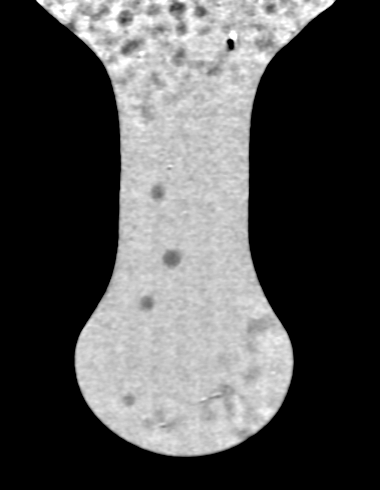
\includegraphics[scale= 0.28]{figures/seg_orig.png}}
%    \mbox{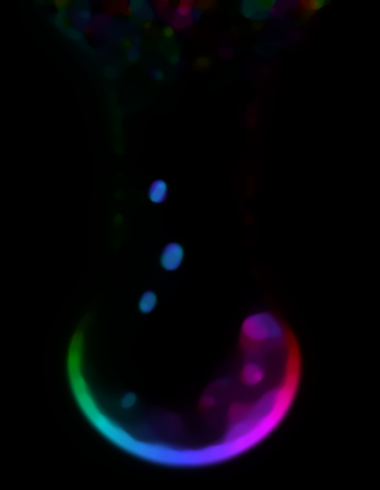
\includegraphics[scale= 0.28]{figures/seg_flow.png}}
%    \mbox{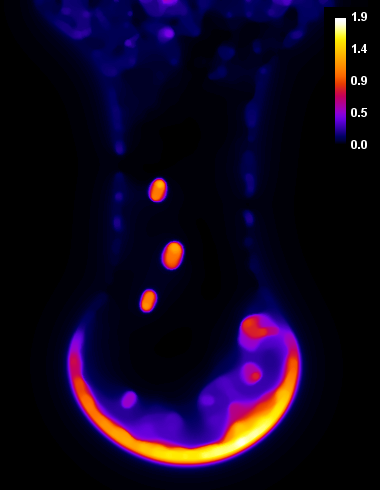
\includegraphics[scale= 0.28]{figures/seg_amp.png}}
%    \mbox{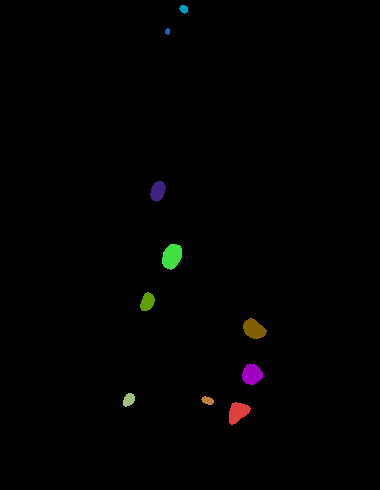
\includegraphics[scale= 0.28]{figures/seg_watershed.png}}
%  }
%
%  \caption[Noise filterst]{ \todo{Enlarge}. Examples of motion-based segmentation. \textbf{Left:} Input image of moving particles (dark spots). \textbf{Middle Left:} Flow field visualized using color-coding (color shows the direction, color brightness shows the magnitude). \textbf{Middle Right:} Segmentation using magnitude of the velocity field. \textbf{Right:} Motion-based segmentation using watershed segmentation on color-coded flow result. Both direction and flow magnitude are taken into account.}
%  \label{fig:motion_segmentation}
%\end{figure*}
%
%
%
%\begin{itemize}
%	  \item Using a flow-related measure as a label
%    \item Using contours?
%    \item Using colors + watershed
%\end{itemize}
       

\subsection{Object Tracking}
\label{tracking}


\textit{Object tracking} is an important task in the field of Computer Vision. It is used for a wide range of applications like video surveillance, human-computer
interaction, automated video analysis and autonomous vehicle navigation. For our application needs we are interested to track and analyses spatio-temporal evolution of various objects imaged by means of X-ray radiation: migrating cells, moving particles, changing structures, etc.


In the most general way, \textit{tracking} is a procedure of estimating the trajectory of an object within an 2D image plane (or 3D volume for tomographic data) as it changes its position over time.  Tracking involves three key steps: detection of moving objects, tracking of these objects within an image sequence, and analysis of their trajectories to learn about their dynamical behaviour.

In order to implement a tracking procedure one should consider a number of important aspects.
First, a suitable representation of the object should be defined. The next aspect is to choose an image feature which will be used to recognize the object. And, finally, an appropriate tracking strategy should be chosen. 

We describe these aspects step by step in the following sections. Note, that the object tracking is a well established and an extensive topic. Here we cover only those approaches which will be implemented within our data analysis framework (see Section \ref{data_analysis}), but additional methods could be  easily incorporated upon the need. For more details we refer the reader to the literature on tracking methods \cite{Yilmaz06, Trucco06}.  


\subsubsection{Object Representation}
\label{tracking_object_representation}

Here we describe common approaches to represent an object shape. In general, the choice of object representation determines the tracking algorithm. It is possible to distinguish the following representations:  
\begin{itemize}
   \item \textit{Points}. The simplest representation of an object is using a point. This point could be, for example, a geometrical center of the object (centroid) or some other characteristic feature. Moreover, complex objects can be represented by a set of points. In general,
a single point representation is well suited for tracking small objects (e.g. particles, cells).

  \item \textit{Primitive geometric shapes}. In this case an object is represented by a simple geometrical shape, such as a rectangle or an ellipse. The motion for such shapes is usually assumed to be described by affine transformations. Such geometrical shapes are useful to represent rigid object.
  
  \item \textit{Object contours}. Contour representation specify the boundary of an
object. This type of presentation is useful for tracking non-rigid objects. The contours are usually described using a special mathematical formulation, known as geodesic active contours or snakes \cite{Caselles95}. However, in the scope of our work we do not use this formulation. Instead, to represent a contour we use a multiple points, distributed on the edge of an object. This simplifies and reduces the number of tracking algorithms in our data analysis framework. 
    
\item \textit{Articulated shape or skeletal models}. Articulated objects are composed of several parts connected together with a joints mechanism. The relations between different parts are driven by a specified kinematic motion model (e.g. angles relations, stiffness). This representation is useful for tracking human or animal body parts. For our class of applications this model can also be useful, however in the current work we do not implement it.
\end{itemize}

As a base representation of objects we opt to choose a point representation, which is general and allows to define small objects with a single point, complex objects as a set of points and non-constant objects contours as a set of points distributed along the boundary of an object. Additionally, this allows us to have only one type of tracking algorithm (see Section \ref{object_tracking}).  


\subsubsection{Features for Tracking}
\label{tracking_features}

The crucial aspect is a choice of image features or object properties which are used for tracking. The requirements for such features are: they should be unique and provide a good description the object, they should also be robust to noise and other artifacts.
The commonly used visual features are:

\begin{itemize}
   \item \textit{Color}. The primary information about an object is its color or a brightness value. In the visual light imaging scenario the color is mainly determined by the illumination conditions of the scene and surface properties of the object (reflectance, diffusivity). In our case, the color represents the result of interaction of X-rays with a sample (e.g. attenuation of the upcoming radiation).  
   
   \item \textit{Edges}. Another characteristic property of an object is its boundaries.
   For this case an edge detection algorithm is used to identify the changes in image intensities, representing an object contour. There are several advantages for this feature. First, the edges are less sensitive to illumination changes. Second, they additionally provide orientational information. There are a number of easy to implement and accurate edge detection techniques available \cite{Canny86, Bowyer01}.   

	\item \textit{Optical Flow}. In this work the main feature used for tracking is a displacement vector computed by an optical flow algorithm. This vector is available for every pixel in the image (dense displacement field) and directly shows the new position of the given pixel on the next frame.

\item \textit{Texture}. Texture is feature which describes brightness variations on the surface or within an object. These variations might be caused by a pattern in the illumination or properties of the object itself. Usually, to quantify the texture a number of texture descriptors are used. Similar to an edge feature, texture based information is also robust with respect to illumination conditions and noise.
\end{itemize}

Depending on the application and available data, a combination of aforementioned features can be used. In the scope of this work we use an optical flow as the main source of information to perform tracking. In order to track contours of non-rigid or complex objects we additional may use the object edges to distribute a set of points for further tracking.  

\subsubsection{Object Tracking}
\label{object_tracking}

After the object representation and features of interest are chosen, the final step for the tracker algorithm is to estimate a trajectory of a moving object by locating its position in every frame of the image sequence.

The tracking procedure starts by detecting or identifying initial position of objects. In our work we mainly use the point representation for small objects and multiple points to represent complex objects. The distribution of points representing an object can be done manually by the user or distributed automatically. In case of automatic selection the points can be distributed randomly, using specified positions on a grid or according to image features discussed in Section \ref{tracking_features}.
 
The model which is selected to represent an object constraints the type of motion or deformation it can perform. For a point representation, the object motion is limited to translations. Tracking of an object represented by a single point is trivial, we just follow each point using a computed displacement vector.
A non-rigid object represented by multiple points defining its contour can move freely. In this case, by analyzing the new positions of the contour it is possible to learn about object's appearance. For a complex rigid object represented by multiple points we may introduce a number of motion constraints  \cite{Yilmaz06} to reconstruct its affine transformation. These constraints are schematically depicted in Figure \ref{fig:motion_constraints}.  
  
\begin{figure*}[ht]
  \centerline{
    \mbox{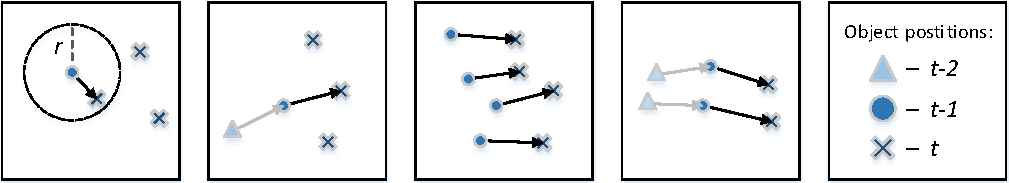
\includegraphics[width=0.98\textwidth]{figures/fig_38_p69.pdf}}
  }

  \caption[Noise filterst]{Different motion constraints. \textbf{Left:} Maximum velocity constrained to the radius $r$. \textbf{Middle Left:} Small velocity change constraint. \textbf{Middle Center:} Common motion. \textbf{Middle Right:} Rigidity constraints. Triangles denote object position at frame $t$-2, circles denote object position at frame $t$ - 1, and crosses  denote object position at frame $t$. \textbf{Right:} Scheme of pixel codes on different time frames. Image adopted from  \cite{Yilmaz06}.  }
  \label{fig:motion_constraints}
\end{figure*}

\begin{itemize}
	\item \textit{Maximum velocity} specifies an upper bound of the object velocity which it can undergo. This can be specified by a circular neighborhood around an object.
	\item \textit{Small velocity change} (temporal motion smoothness) assumes the direction and magnitude of the object's displacement does not change rapidly.
	\item \textit{Common motion} (spatial motion smoothness) constrains the displacements of nearby points within the object to be similar.
	\item \textit{Rigidity} assumes that objects are rigid, resulting that the distance between
any two points which belong to the object are unchanged after the .
\end{itemize}



%\subsection{Temporal Changes Detection}
%\label{temporal_changes_detection}
%
%Small overview for Temporal changes detection methods. The general task for Temporal changes detection.
%
%\subsubsection{Motion Compensated Difference}
%
%
%\begin{itemize}
%	\item Problem statement
%  \item Motivation
%  \item Limitations of Difference approach
%  \item The task for temporal changes detection method
%\end{itemize}


\subsection{Image Registration and Alignment}
\label{image_registration}


\textit{Image registration} is a process of aligning two or
more images of the same scene taken at different times,
from different views, or by different imaging techniques.  Registration is required in many fields, such as remote sensing, in medicine and in Computer Vision. An example of image registration of time-resolved tomographic data is shown in Figure \ref{fig:example_registration}.


%\begin{figure*}[ht]
%  \centerline{
%    \mbox{\includegraphicslabeledw[scale= 0.53]{figures/example_registration_a.png}{a}}
%    \mbox{\includegraphicslabeledw[scale= 0.53]{figures/example_registration_b.png}{b}}
%    \mbox{\includegraphicslabeledw[scale= 0.53]{figures/example_registration_c.png}{c}}
%    \mbox{\includegraphicslabeledw[scale= 0.53]{figures/example_registration_d.png}{d}}
%  }
%  
%  \vspace{3pt}
%  
%  \centerline{
%  	    \mbox{\includegraphicslabeledw[scale= 0.53]{figures/example_registration_e.png}{e}}
%  	    \mbox{\includegraphicslabeledw[scale= 0.53]{figures/example_registration_f.png}{f}}
%  	    \mbox{\includegraphicslabeledw[scale= 0.53]{figures/example_registration_g.png}{g}}
%  	    \mbox{\includegraphicslabeledw[scale= 0.53]{figures/example_registration_h.png}{h}}
%  }
%  \caption[Noise filterst]{Example of image registration using optical flow. Application: \textit{in-situ} analysis of void formation in flip-chip devices under electrical load. \textbf{(a)} First time frame of the image sequence. \textbf{(b)} Second frame. \textbf{(c)} Changes detection using image difference. Global sample movement cause a lot of falsely identified regions. \textbf{(d)} Image difference after image registration via optical flow. \textbf{(e-h)} After the image registration is performed, the tracking of voids evolution is possible . Colors show individual pores. Note, that all voids merge into a single one in the end of a sequence.}
%  \label{fig:example_registration}
%\end{figure*}

The task for image registration is to find the optimal  spatial and intensity transformations so the input images are matched. Image registration can be defined for two-dimensional images as a mapping between a target $I_1(x, y)$ and a reference $I_2(x,y)$ images, where $I(x,y)$ represents image intensity. Then, the mapping between these images can be expressed as following:
$$I_2(x,y) = g(I_1(f(x,y))),$$
where $f$ is a function which maps spatial coordinates $(x,y)$ into new locations $(x',y')$, such as $(x', y') = f(x,y)$ and $g$ is an intensity transformation.

Depending on the task and application field, it is possible to distinguish four classes of specific registration problems:
\begin{itemize}
\item \textit{Multimodal registration (different sensors)}: Registration of images of the same scene acquired using different imaging modalities. Example: Combine structural information form CT and functional brain activity from MRI imaging.

\item \textit{Template matching}: Match a reference pattern or a model with an image. Example: Registration of an image pattern with the model representation of the scene or atlas. 

\item \textit{Viewpoint registration (different views)}: Registration of a scene taken from different viewpoints. Example: Depth or shape reconstruction in Computer Vision.
 
\item \textit{Temporal registration}: Registration of images of the same scene taken at different time, under different imaging or physical conditions. Example: Detection and monitoring of changes in a scene, object or specimen.

\end{itemize}
In our work we mainly focus on the task of temporal registration to expose changes between subsequent images or perform image alignment of object position.

In general, image registration procedure consist of the four stages \cite{Zitova03}, which are similar to the common steps for object tracking (see Section \ref{tracking}):
\begin{itemize}

\item \textit{Feature detection}. Detection of salient and distinctive features such as objects, characteristic points, edges, contours, lines, corners, etc.
Such features can be placed manually or detected automatically.

\item  \textit{Feature matching}. Establish the correspondence between the features detected in the target and the reference image. To perform a matching procedure a number of spatial constraints and similarity measures are used.  

\item \textit{Transformation estimation}. A mapping between the target and the reference image is estimated according to established feature correspondences. 

\item \textit{Image resampling and transformation}. As a final step, the images are transformed towards each other using the estimated mapping function. For the mapping and resampling of intensity values an appropriate interpolation techniques is used.

\end{itemize}

All the differences within images in terms of pixel positions or intensity values due to the temporal changes or different acquisition conditions are referred as \textit{variations}.
It is important to distinguish between distortions and other variations. \textit{Distortions} are variations which are the source of misregistration.  Essentially it is the distortions between images which we would like to remove by registration procedure and reveal the changes of interest.
These distortions might be caused by the image noise, intensity changes, sample or detector movement or other unwanted effects \cite{Zitova03}.

Another important aspect, is to distinguish between global/local transformations and
global/local variations \cite{Brown92}.  A global transformation is described by the same mapping (e.g. single equation) and transforms the whole image. A local transformation maps different pixels according to their spatial localization.
The same holds for variations: some variations are due to the global process like camera misalignment or global sample movement, and some variations correspond to local differences.
To perform image registration it is crucial to take into account which kind of transformation is applied for which kind of variations. For instance, images may have local variations, but a global transformation can be used to align for a global change to assist in revealing small local changes.
We will cover these aspects in a Section \ref{image_registration_strategies} where we discuss different registration strategies. In the following section we describe all the relevant steps in image registration.



\subsubsection{Feature Detection}
\label{reg_feature_detection}

A crucial step for image registration is the selection of feature descriptors.
These features should be distinct, well distributed over the image and robust under different image artifacts (e.g. noise, brightness changes, artifacts).
It is possible to categorize most of the registration techniques according to feature detection approach in the following way: 
\\
\\
\textit{Area-based detection}. Area-based methods do not perform a separate feature detection step. Instead, these approaches perform the feature matching procedure directly, according to a specific similarity measure. We discuss these methods in the next Section \ref{reg_feature_matching}.
\\
\\
\textit{Feature-based detection}. This approach is based on the detection of salient and distinctive feature to perform image registration.  Whole range of characteristic information extracted from the image data can be used for this purpose. Such features might include: specific points, lines, corners, contours, texture, geometric shapes, etc. An important difference from the area-based methods is that this kind of features represent higher level of information and could correspond to a physical model of the scene. 
The procedure for feature detection is closely related to the similar task for object tracking discussed in Section \ref{tracking_features}, so the same set of feature detection tools might be used.






\subsubsection{Feature Matching}
\label{reg_feature_matching}

After the features are detected, the next step is to perform feature matching.
In this section we describe the methods which will be used in the scope of this work.
\\
\\
\textit{Area-based matching}. A first category of methods are called area-based methods.
Such methods are also known as \textit{correlation-like}
methods or template matching techniques \cite{Zitova03}. As we already mentioned in the previous Section \ref{reg_feature_detection}, these techniques combine the feature detection and matching procedures. The images are registered without characteristic data points, instead the whole image domain is used.

A classical approach for area-based registration is a \textit{cross-correlation}, which is a statistical method to find similarity between images.  For a template $T$ and target image $I$, the two-dimensional cross-correlation function estimates the similarity for each translation $(u,v)$ by:
$$ CC(u,v) = \sum_{x,y} T(x,y) I(x-u, y-v)). $$
If the best template match with a target image is given at a translation of $(i,j)$, the cross-correlation function will have its peak at $CC(i,j)$.

In the case, if the brightness of the image and template differs due to the varying  imaging conditions, the images can be first normalized. The normalized cross-correlation is then given by:
$$NCC(u,v) = \frac{\sum_{x,y} (T(x,y) - \mu_T) (I(x-u, y-v) - \mu_I)}{\sqrt{\sum_{x,y} (T(x,y) - \mu_T)^2 (I(x-u, y-v) - \mu_I)^2}}, $$
where $\mu_T$ and $\mu_I$ are mean values of the template $T$ and the image $I$ respectively.  

A similar, but more intuitive measure computes the sum of the squared differences (SSD) between a template and an image:
$$SSD(u,v) = \sum_{x,y} (T(x,y) - I(x-u, y-v))^2.$$

Another variant of area-based techniques is the so-called sequential similarity detection algorithm (SSDA). Which simply estimates an absolute differences between two images being matched.
This measure is given by:
$$SSDA(u,v) = \sum_{x,y} |T(x,y) - I(x-u, y-v)|.$$


Area-based techniques are useful for images which are misaligned by rigid transformation, preferably a translation. For more complex geometrical transformation (e.g. fast rotation) the model should be modified, which usually leads to a significant increase in computation load due to the extended search space. Another disadvantage of the area-based methods is a poor performance for noisy data or homogeneous images  without prominent details or structures. In these cases no distinct peak position could be estimated. For example, low-contrast data with noisy background or rotated spherical shape of the embryo with a lot of similar cell structures.
\\
\\
\textit{Feature-based matching}. For this class of techniques we assume that features in the reference and the target images are detected. The next step for feature-based matching is to establish correspondences between them.
There are a vast variety of methods to find such correspondences. We do not contemplate to describe  these algorithms. For the extensive overview of different matching techniques we refer the reader to surveys on image registration methods \cite{Brown92, Zitova03}.
One popular choice of feature-based matching technique is based on scale invariant feature transform (SIFT) \cite{Lowe04}. These methods show good performance for a broad range of transformation models between images. However, their use exceeds the scope of the current work.
In this work the feature correspondences for sparse or dense points are provided by the optical flow method and described by the computed displacement vector.


    
\subsubsection{Transformation Estimation}
\label{transform_estimation}

After correspondences between features are established
the mapping function which overlays the target image with the reference is constructed.
The key component of the registration procedure is a type and properties of a spatial transformation which implements such alignment.
 Since a wide range of transformation types may present within each image, the registration technique is restricted by a particular transformation model or parameters.
This transformation should remove only those image variations, which are the result of distortion and should be corrected. Other image difference (changes of interest) should remain unaffected be the registration procedure and will be used for further analysis. 

As we already disccussed in the Section \ref{image_registration}, transformation can be global and local.  The most common types of global transformations
are rigid, affine, projective, perspective
and polynomial. Within our work the most useful model is rigid transform, which we use to track  
objects that preserve their shape. Affine transformation is a more general type of transformation and includes translation, rotation, scaling, similarity transformation, reflection, shear mapping, and compositions of them.  Here we enlist three main transformation models:
\\
\\
\textit{Global mapping models}.
The most common global transformation is a rigid transform, which preserve all the geometric properties of the object. According to this transform each point $(x_1,y_1)$ of the first image is mapped to a point $(x_2, y_2)$ of the second image in the following way:

$${x_2 \choose y_2} = {t_x \choose t_y} + s
 \begin{pmatrix}
  \cos \theta & -\sin \theta  \\
  \sin \theta & \cos \theta \\
 \end{pmatrix} {x_1 \choose y_1},$$
where $t_x, t_y$ are translation vector components, $\theta$ is a rotation angle and $s$ is a scale factor. A rigid transform with a scaling factor could be useful to register datasets acquired with a cone beam geometry (with different object to beam distances). 


To estimate a transformation and its parameters global mapping methods based on point matching use a set of point correspondences. In this case, if a sufficient number of control points are provided, it is possible to derive the parameters of the transformation using two general methods: 
\begin{itemize}
\item \textit{Approximation} procedure estimates the overall transformation mapping in such a way, that matched points are aligned as close as possible. This is usually implemented with statistical optimization methods, e.g. least square approximation. The key assumption in this case, is that the matched points could be inaccurate, so the transformation should satisfy all the matches in an optimal way.
   
\item \textit{Interpolation} procedure finds the transformation mapping so the feature points match precisely and parameters in other locations are estimated using a special relation. This method is useful in the case if fewer, but more accurate matches are provided.    
\end{itemize}


\noindent \textit{Local mapping models}.
A significant drawback of global approaches is that these methods do not properly treat the transformations which are local. For this case a number of specific or modified registration methods are used. 
In this work we do not use this type of mapping models, so we opt to skip the description of such techniques.  For the overview of available methods the reader is referred to the works of \cite{Brown92, Zitova03}.
\\
\\
\textit{Elastic registration}.
A fundamentally different approach for the registration of images with
complex or local distortions is not to use
any parametric or global mapping functions.
The idea of \textit{elastic registration} was introduced in a seminal work of Bajcsy and Kovacic \cite{Bajcsy89}. In this method an image is represented as an elastic model (rubber-like) and transformations are described as deformation forces constrained by a stiffness or smoothness.
In the current work we use the results of optical flow to compute dense local displacements to perform elastic registration. In our case the data constancy assumption is serving as a metric for feature matching and smoothness constraint is a similar concept as in the case of elastic registration. Note, that the optical flow parameters should be chosen appropriately, depending on the task and amount of local variations to be corrected or revealed. 
   

\subsubsection{Image Resampling}

To apply a mapping transformation, which is computed in the previous steps, an appropriate image resampling and interpolation have to be employed. This transformation can be done in a forward and backward direction. The forward approach is hard to implement and could produce data outliers (hole or overlaps) due to multiple mapping or discretization problems. The backward registration is easier to implement and produce good results. 

There is a large number of choices for the interpolation procedure \cite{Parker83, Grevera98}. 
For our task we use a backward registration by means of bilinear interpolation described in Section \ref{compensation}. For the volumetric data we use a 3D variant of this transformation - trillinear interpolation.

\subsubsection{Image Registration Strategies}
\label{image_registration_strategies}


Here we summarize several strategies of image registration used in our data analysis framework:
\begin{itemize}
  \item \textit{Dense local registration via optical flow}. Features - dense pixels, matching procedure - dense optical flow,  transformation -  backward flow field interpolation. Application example: Register two images to obtain the maximum similarity. 
  \item \textit{Dense global registration via optical flow}. Global registration is achieved by using a coarse representation of the flow field or input images, i.e. using an increased smoothness constraints or presmoothing parameter. Features - dense pixels, matching procedure - optical flow, transformation - backward flow field interpolation. Application example: Register two images of the same scene to compensate for global elastic changes to reveal local changes. 
  \item \textit{Feature-based registration via optical flow}. Features - sparse set of landmarks, matching procedure - sparse optical flow correspondences, transformation - global transformation based  on approximation or interpolation (see Section \ref{transform_estimation}). Application example: align images based on automatically distributed landmarks.
  \item \textit{Global image registration with correlation-based technique}. Features - entire image (image-based matching) , matching procedure - correlation-based techniques (SSDA is a good choice, see Section \ref{reg_feature_matching} ).  Application example: align images to compensate for a global sample movement prior to the optical flow computation, which is sensitive for small changes.
\end{itemize}






%--------------------------------------------------------
%\section{[OPTIONAL] Visualization Methods}
%\label{visualization}
%--------------------------------------------------------

%The section gives a brief survey on existing visualization methods for time-varying data.
%The focus is on the practical use of the techniques for particular data analysis tasks.
%Examples of possible applications are also discussed.
%
%\subsection{Vector Field}
%
%[pages 1-2]
%
%\begin{figure*}[!ht]
%  \centerline{
%    \mbox{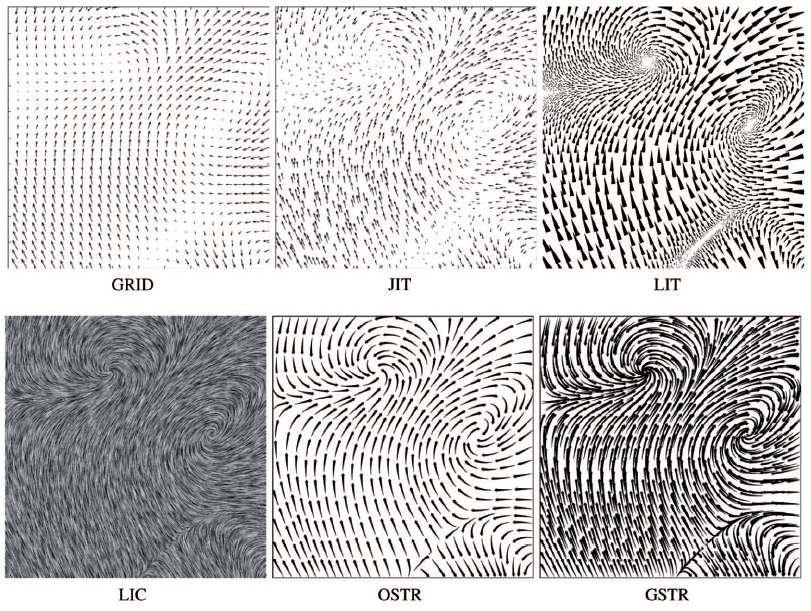
\includegraphics[scale= 0.55]{figures/vector_viz_types.png}}
%  }
%  \caption[]{\textbf{Left:} First frame of original image. \textbf{Middle:} With Gaussian noise.  \textbf{Right:} Parameter +2. Image source: \cite{Laidlaw05}}
%  \label{fig:lookup_tables}
%\end{figure*}
%
%\comment{Include information from vector fields visualization paper}
%        
%\begin{itemize}
%	\item Name
%  \item Description, Shows what?
%  \item Example image
%  \item Best usage examples
%\end{itemize}
%
%        
%\subsection{Scalar Field}
%
%[pages 0.5-1]
%
%\begin{itemize}
%	\item Name
%  \item Description, Shows what?
%  \item Example image
%  \item Best usage examples
%\end{itemize}
%
%
%Scalar field as a N-dimensional image can be repsesented in different color codes or Lookup tables (LUTs). 
%\change{From. Russ. Lookup tables (LUTs) can be implemented either in hardware or software. They use the original
%value as an index into a stored or precalculated table, which then provides the derived
%value. This process is fast enough that acquisition is not affected. LUTs
%are also used for displaying stored images, particularly to substitute colors for gray scale
%values to create pseudo-color displays.}
%
%\change{From. Russ.The use of color to encode richly multidimensional information must be distinguished from
%the very common use of false-color or pseudo-color to substitute colors for brightness in
%a monochrome image. Pseudo-color is used because of the limitation mentioned before in
%the visual ability to distinguish subtle differences in brightness. The use of color scales as a substitute for brightness values allows us to show and see small
%changes locally, and identify the same brightness values globally in an image. This should be
%a great benefit, since these are among the goals for imaging discussed below. Color might be used  to encode flow components, velocity, differently moving objects and other quantitative.
%These uses generally have little to do with the properties of the image and simply take advantage
%of the human ability to distinguish more colors than gray scale values.}
%An example of color coding using different LUTs is given in Figure \ref{fig:lookup_tables}.
%
%\begin{figure*}[!ht]
%  \centerline{
%    \mbox{\includegraphics[scale= 0.8]{figures/lookup_tables.png}}
%  }
%
%  \caption[Noise filterst]{\todo{Change image}. Taken from \cite{Russ11}. \textbf{Left:} First frame of original image. \textbf{Middle:} With Gaussian noise.  \textbf{Right:} Parameter +2.}
%  \label{fig:lookup_tables}
%\end{figure*}
%
%
%\subsection{Line Convolution}
%
%[pages 0.5-1]
%
%\begin{itemize}
%	\item Name
%  \item Description, Shows what?
%  \item Example image
%  \item Best usage examples
%\end{itemize}
%
%\subsection{Flow Streamlines}
%
%
%\begin{itemize}
%	\item Name
%  \item Description, Shows what?
%  \item Example image
%  \item Best usage examples
%\end{itemize}
%
%\subsection{Color Coding}
%
%Link: http://hci.iwr.uni-heidelberg.de/Static/correspondenceVisualization/
%
%To show:
%\begin{itemize}
%	\item 2D Bruhn colors
%	\item 2D Middl colors
%  	\item 3D RGB cube
%  	\item 3D projections: XY, YZ, XZ
%  	\item Simplified colors: 6, more
%\end{itemize}
%
%
%%\subsection{[OPTIONAL] Texture and Shape Coding}
%%
%%\comment{Find examples and code for texture-based coding}
%%
%%\begin{itemize}
%%	\item Name
%%  \item Description, Shows what?
%%  \item Example image
%%  \item Best usage examples
%%\end{itemize}
%
%\subsection{[OPTIONAL] Comparison of Visualization Methods}
%
%Comparison table of visualization methods. 
%Parameters to compare:
%\begin{itemize}
%	\item Direction
%    \item Magnitude
%    \item Density
%    \item Time evolution (like trajectories). Think about it. Check info in Vectors paper
%    \item 3D version
%\end{itemize}
%
%
%
%%--------------------------------------------------------
%\section {[OPTIONAL] Scientific software}
%%--------------------------------------------------------
%
%Section outline is here. \comment{Put the section here or to Appendix? Or skip completely?}
%
%\comment{Check Nature methods paper: Visualization of image data from cells to organisms}
%
%Description scheme:
%\begin{itemize}
%    \item Name
%    \item Short description
%    \item Features
%    \item Screenshot with visualization
%\end{itemize}
%    
%Comparison table in the end. TODO: Make a list of parameters to estimate.
%
%List of software to present:    
%\begin{itemize}
%	\item  ImageJ
%  \item  VTK
%  \item  Avizo/Amira
%  \item  Volume Studio MAX
%  \item  VisIt
%\end{itemize}



%******************************************************************
%******************************************************************
\chapter {Computational Framework}
\label{software}
%******************************************************************
%******************************************************************

In this chapter we describe our computational framework. First, we present the software architecture which is implemented as a modular approach. Then we describe main responsibilities of individual components of each module.
The second part is devoted to high performance computing. First, we show a number of efficient numerical techniques to speed up the computation process. Then we present an implementation of optical flow methods on graphical processing units (GPUs), which enables us to process large datasets in a reasonable time. In the last part of the chapter we describe visualization methods which are implemented in our data analysis framework.


%--------------------------------------------------------
\section {Software Framework}
\label{software_framework}
%--------------------------------------------------------

The software for optical flow computation and time-resolved data analysis is implemented using C++ programming language, is modular and follows the object-oriented design paradigm. The requirements for our implementation are high performance, platform independence and strict control for types and memory management.
Most of the components are implemented within a single unified framework, if not stated otherwise (e.g. some data analysis or data visualization packages are implemented as external routines). In the following section we describe all the software components in more details.


\subsection {Modules}

Our optical flow computation and data analysis framework is designed as a modular system. Each module is responsible for a specific class of functionality. A central part of the framework is a \texttt{CORE} module, which contains classes and methods to perform the optical flow computation. The integral class of this  module is a \texttt{Runner} class which serves as unifying interface and control routine between the core classes and external modules. 
With such organisational architecture it is possible to minimize interdependence between different parts. It also allows to simplify easily the extension or modification of the existing functionality.
The overall diagram of our framework is presented in Figure \ref{fig:software_scheme}.

\begin{figure}[h]
	\centering
	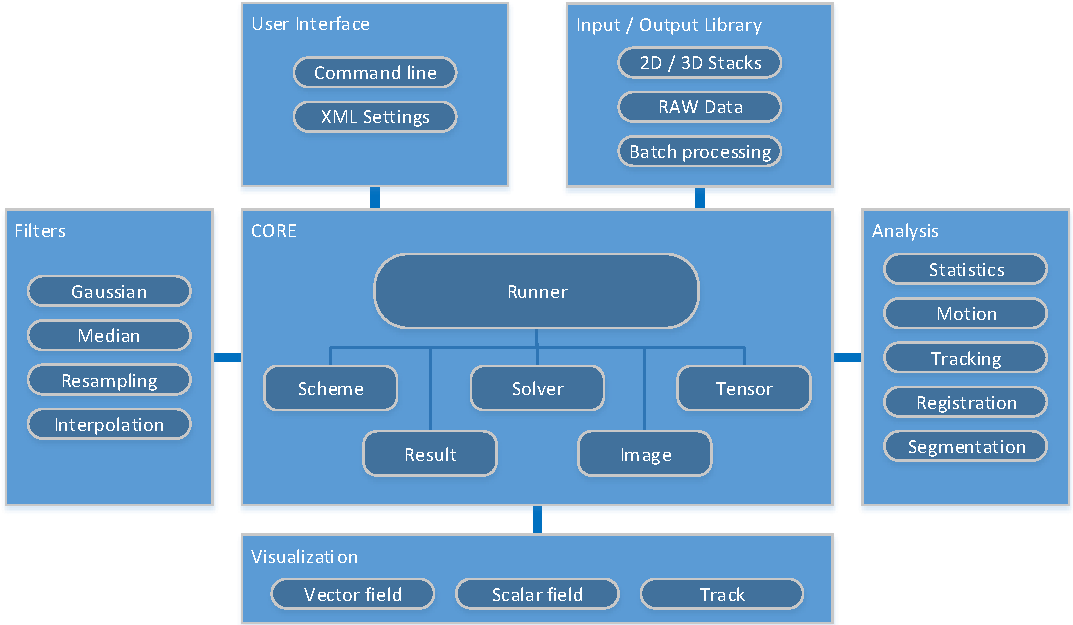
\includegraphics[scale=0.87]{figures/software_scheme.pdf}
	\caption{Optical flow computation and data analysis framework as a modular system. Each model is responsible for a specific class of functionally.  All modules are connected and controlled via the \texttt{Runner} class of the \texttt{CORE} module.}
	\label{fig:software_scheme}
\end{figure}

The developed software framework consists of the following modules:
\begin{itemize}
	\item User interface
	\item Input / Output Library
	\item Filters
	\item Core
	\item Analysis
	\item Visualization	
\end{itemize}

In the following part we describe the responsibility and essential functionality of each of these modules.
\\
\\
\textit{User Interface Module}. Provides an universal interface to setup and adjust the overall workflow, select optical flow models, adjust computation parameters, as well as perform further analysis of the optical flow results. It is implemented as a command line utility and a settings file in a easy-to-read XML format\footnote{\url{http://www.w3.org/XML/}}. 
\\
\\
\textit{Input / Output Library Module}. The module provides routines for data input and output. This includes the work with settings files, statistics, image data, resulting vector fields and other related information. The library allows to use the following data inputs:
\begin{itemize}
	\item 2D / 3D image sequences using common image formats.
	\item RAW data. Using various data types: 8-bit, 16-bit, 32-bit. 
	\item Batch processing. Allows to perform batch processing of long image sequences. Several input modes are possible: masking mode with the specified image indexes; a list of images; a list of image pairs. 
\end{itemize}

\textit{Filters Module}. The module contains various filter which are used during preprocessing, data analysis or optical flow computation. The list of possible image filters includes:
\begin{itemize}
	\item Gaussian smoothing. Implements image filtering via convolution with a Gaussian function  (See Section \ref{noise_filters}).
	\item Median filtering. Implements image filtering using a median filter (See Section \ref{noise_filters}).
	\item Image resampling. Using a number of methods: Averaging, Area-based resampling.
	\item Image interpolation. Available modes: nearest-neighbor, bilinear, trilinear, bicubic interpolations \cite{Parker83}. 
\end{itemize}

\textit{Core Module}.  This module is the central part of the framework and contains classes and methods to perform the optical flow computation, as well as to connect and control the classes from external modules. 
\begin{itemize}
	\item Image. Provides functionality to represent an image in various formats and dimensions. The implemented types of images are: \texttt{Image2D} \texttt{Image3D} and \texttt{ImageRGB}.
	\item Scheme. The main class to impose data constancy assumption via the computation of a motion tensor (See Section \ref{data_constancy_assumptions}). 
	\item Tensor. The class stores the entries of a motion tensor for 2D or 3D image data.
	\item Solver. The main class which performs numerical solution of the optical flow problem via solution of linear equations, which describe the minimum of the energy functional.
	\item Result. This class stores the results of optical flow computation and contains methods to analyze them. In our framework two versions of the optical flow results are implemented - \texttt{Result2D} and \texttt{Result3D} - for two-dimensional and three-dimensional cases respectively.  
\end{itemize}

\textit{Analysis Module}. Contains a set of routines for further analysis based on optical flow results. Some functionality implemented within the same framework and some as external tools.
\begin{itemize}
	\item Motion. A set of methods for further analysis of displacement fields. See Section \ref{motion_analysis} for theoretical description and Section \ref{component_motion} for the list of available functionality. 
	\item Tracking. A module for points or objects tracking using the computed displacement fields as a  feature (See Section \ref{tracking_features}). 
	\item Registration. A module for motion-based image registration (See Section \ref{image_registration}).
	\item Segmentation. Module for motion-based segmentation of moving objects. Thresholding methods are implemented as part of our framework, more advanced methods such as region-growing and level sets methods are implemented externally using Fiji / ImageJ software\footnote{\url{http://imagej.net}}. 
\end{itemize}




\subsection {Components}

%\subsubsection {Hierarchy of Software Components}
%
%\todo{Make figure: All components, interaction}

\subsubsection {Scheme Components}

Scheme components intend to perform the construction of a data term by computation of the corresponding motion tensor (See Section \ref{data_constancy_assumptions}).
A list of available data constancy assumptions implemented as separate \texttt{Scheme} classes includes:
\begin{itemize}
	\item \texttt{Scheme}\texttt{[DataConstancy]}. Performs a computation of a motion tensor for a given constancy assumption. The complete list of available constancy constraint is presented in Section \ref{data_constancy_assumptions}. The implemented constancy modes are \texttt{DataConstancy} = \{\texttt{Grey}, \texttt{Gradient}, \texttt{GreyGradient}, \texttt{GradientNorm}, \texttt{Laplacian}, \texttt{LogDerivatives}, \texttt{GreyRGB}, \texttt{GradientRGB}\}.
	  
	\item \texttt{SchemeNormalization}. All the previously presented data constancy assumptions (list \texttt{DataConstancy}) can be normalized according to the procedure described in Section \ref{normalization}.
	
	\item \texttt{SchemeCLG}. All data assumptions \texttt{DataConstancy} can be convolved with the Gaussian function to obtain a motion tensor which integrates the local information, to obtain the so-called Combined-Local-Global approach (See Section \ref{clg}).
	
	\item \texttt{SchemeMultiChannel}. This scheme allows to construct a data term using an arbitrary number of channels as the input (for example, 3-channel RGB color images). This might be useful to incorporate images obtained using multiple contrast modalities.
	
	\item \texttt{Scheme3D}. All the presented schemes can be implemented for 2D or 3D images. Moreover, implementation for higher dimensions can be extended in a straightforward way.
\end{itemize}


\subsubsection {Solver Components}

The \texttt{Solver} classes perform numerical computation of the optical flow problem, solving a system of  linear equations. Several algorithms are available in our computational  framework (See Section \ref{iterative_methods}): 

\begin{itemize}
\item \texttt{SolverJacobi}. Performs solution of a system of linear equations using a Jacobi method (see Section \ref{jacobi_method}). It is not an optimal solver methods in terms of performance and requires large amount of iteration to converge to the optimal solution. However, for the case of parallel computations, where each element of the matrix is evaluated separately, this solver is more suited (see discussion in Section \ref{jacobi_method}). 

\item \texttt{SolverGauss}. Solves a system of linear equations using a Gau\ss-Seidel method presented in Section \ref{gauss_method}. It speed ups the computation time comparing with the Jacobi methods, since all the entries of the approximation matrix are updated on each iteration. 

\item \texttt{SolverSOR}. Performs the solution using a Gau\ss-Seidel method with the successive overrelaxation technique, which is presented in the section dedicated to the advanced numerical techniques (see Section \ref{sor_method}).

\item \texttt{SolverMultiLevel}. This solver implements a multi-level computation as described in Section \ref{multilevel} and allows to perform high accuracy optical flow computation of large displacements. On each individual computation level the \texttt{SolverJacobi}, the \texttt{SolverGauss} or \texttt{SolverSOR} numerical solvers can be used.

\end{itemize}


\subsubsection {Results Components}
\label{components_results}

The responsibility of this module is to store and analyze the results of optical flow computation.
The following measurements are implemented:

\begin{itemize}
	\item \texttt{EndpointError}. This measure is used to compare two vector fields in terms of a distance between two vectors (See Section \ref{endpoint_error}). Presently it is the most popular measure to compare the computed results with a ground truth displacement field.  
	
	\item \texttt{AngularError}. Computes the angular differences between two vectors (See Section \ref{angular_error}).
	
	\item \texttt{DataConstancyError}. Computes a confidence measure based on the data constancy error (See Section \ref{data_constancy_error}).
	
	\item \texttt{EnergyError}. Computes a confidence measure based on the residual energy of the energy functional (See Section \ref{energy_based_measure}).
	
	\item \texttt{UniquenessError}. Computes a confidence measure based on the motion uniqueness criteria (See Section \ref{motion_uniqueness_criteria}).
	
	\item \texttt{ConsistancyError}. Computes a confidence measure based on the constancy between forward and backward flow fields (See Section \ref{forward_backward_check}).
	
	\item \texttt{PredictionError}. Computes a confidence measure based on the optimal prediction principle (See Section \ref{optimal_prediction_principle}).
	
	\item \texttt{ErrorStatistics}. For each of the error or confidence metrics presented above, a complete set of statistical measure is extracted and can be used. These measures include a minimum (\texttt{min}), a maximum (\texttt{max}), a mean (\texttt{avg}) and standard deviation (\texttt{std}). Moreover, for the endpoint error metrics a set of robust statistics measures is also available. They compute the percentage of pixels that have an error measure larger then a certain amount of pixels. In particular, we compute \texttt{R0.5}, \texttt{R1.0}, and \texttt{R2.0} for the endpoint error, which corresponds to half, one and two pixels error respectively.  
	
	\item \texttt{ErrorRegions}. For every error or confidence metric it is possible to evaluate their statistics in various image regions to get insights how optical flow methods perform in these regions. We provide the following regions of interest: whole image (\texttt{All}), around motion discontinuities (\texttt{Disc}), in textureless regions (\texttt{Untext}), around data artifacts (\texttt{Err}) or in an arbitrary region (\texttt{Roi}). All the regions of interest have to be supplemented to the results analysis routine as binary masks.
	
\end{itemize}

\subsubsection {Motion Analysis Components}
\label{component_motion}

These routines allow to perform further analysis of the computed motion field. The following methods are implemented within our analysis framework:
\begin{itemize}
	\item \texttt{Magnitude}.  See Section \ref{magnitude}.
	
	\item \texttt{Phase}. See Section \ref{phase}.
	
	\item \texttt{Curl}. See Section \ref{curl}.
	
	\item \texttt{Divergence}. See Section \ref{divergence}.
	
	\item \texttt{Components}. The module allows to save individual components of the computed flow field for further analysis.
	
	\item \texttt{Kinematics}.  Allows to extract kinematics components from a motion field. Under assumption of a rigid motion this computational module requires as an input a set of landmarks representing the object of interest, a center of coordinates and an axis of rotation. As an output the component produces a translational (\texttt{trans}) and rotational components (\texttt{rot}) of the object's motion. An example of such motion analysis is presented in Section \ref{app_kinematics_insects}.  
\end{itemize}


\subsubsection {Tracking Components}

These components perform object tracking or tracking of individual points using the results of optical flow computation. With the help of these routine it is possible to perform the following tracking operations:
\begin{itemize}
	\item \texttt{Tracks}. The tracking component takes as an input a set of initial points (landmarks) and performs the tracking procedure using the results of optical flow throughout an image sequence, specified by a number of frames. As an output a list of points and their coordinates on each time frame is produced. A possibility to filter the resulting tracks according to confidence measures, e.g. a consistency measure (See Section  \ref{components_results}), or according to the total distance is also available. An example of this tracking procedure is presented in Section \ref{app_kinematics_insects}. 
	
	\item \texttt{TracksAmira}. The same as the previous methods, but saves the output in a format compatible with the Amira/Avizo software\footnote{\url{http://www.fei.com/}}.
	
	\item \texttt{TracksVTK}. The same as the previous methods, but saves the output in a Visualization Toolkit (VTK) format\footnote{\url{http://www.vtk.org/}}. 
\end{itemize}


%\subsubsection {Temporal Changes Components}













%--------------------------------------------------------
\section {High Performance Computing}
\label{performance}
%--------------------------------------------------------

In this section we discuss such an important aspect as high performance computing. Since optical flow methods are very computationally demanding, an efficient implementation of these techniques should be provided to guarantee that the data processing on a given computational platform is feasible.

First, we discuss several numerical techniques, which allow to speed up the computation time. Then we focus our attention on the implementation of optical flow methods on the GPU architecture.


\subsection{Numerical Schemes}
\label{advanced_numerics}

\subsubsection{Successive-Overrelaxation}
\label{sor_method}

The convergence speed of the Gau\ss - Seidel method can be substantially improved by performing \textit{Successive Overrelaxation} (SOR) technique \cite{Yo71, Saad03}. This is done via extrapolation of the Gau\ss-Seidel result. If we denote by $\bar{\textbf{x}}$ the result of Gau\ss - Seidel method for the iteration step $k+1$, the SOR technique then given by:
$$ \textbf{x}^{k+1}_i = (1-w) \textbf{x}^k_i + w \: \bar{\textbf{x}}^{k+1}_i ,$$
where $w \in [0,2)$ is a \textit{relaxation} parameter.  
Then, The Gau\ss-Seidel method can be extended by the overrelaxation technique in the following way:
$$ x^{k+1}_i = (1-w) x^k_i + w \frac{1}{a_{i,i}} (b_i - \sum_{j < i} a_{i,j} x^{k+1}_j - \sum_{j > i} a_{i,j} x^{k}_j) $$
For the value of relaxation parameter $w=1$, the SOR method comes down to the original Gau\ss-Seidel method. The choice of the relaxation parameter has a strong influence on the convergence speed. A parameter $w$ smaller then 1.0 allows to perform underrelaxation which could lead to improved stability of the algorithm. For the values larger then 1.0 the method performs overrelaxation of the result and thus accelerate the convergence. An optimal value of the relaxation parameter should be chosen according the the specific task. For our applications we select values which are close to the maximum value, such as $w \in [1.9..1.95]$.
A major drawback of the method is a possible oversmoothning of the resulting displacement fields. 


\subsubsection{Adaptive multi-level strategy}

An interesting approach to decrease the computation time is to reduce the input on each computation level. For this purpose the computed flow field is evaluated according to a special criteria. For example one may use the fact that the flow field id varying slowly form one computation level to another. This may highlight that the correct flow has already been estimated. In such regions the computationally expensive energy minimization is substituted by a simple interpolation from the results of previous computation levels. Such approach was presented by the authors in \cite{CGF3013} and allowed to significantly reduce the computation time without serious impact on the accuracy of the overall result. This approach can be especially advantageous for datasets with small or isolated objects and dominance of the static background. In this cases an adaptive computation procedure removes most of the irrelevant computations in the background region.    


%\subsubsection{Combining Different Algorithms}
%
%\todo{Give reference to Fusion Flow paper}
%\comment{Add information about combination of efficient and fast implementation with a successive run of high precision OF implementation . From \cite{CGF3013} Show references}
%



\subsection{GPU Computing}   
\label{gpu} 


This section is dedicated to a GPU-based implementation of the optical flow algorithm. First, we briefly discuss the key features of the GPU architecture \cite{nvidiatoolkit, nvidia2010developer}. Then we introduce a GPU-based implementation that uses only one GPU device and is limited to the datasets that can be fitted in the GPU memory. The main aspects of the implementation are discussed in details. Finally, we show how a single GPU device version can be extended in order to process arbitrary large datasets.


%--------------------------------------------------------
\subsubsection{GPU Computing Architecture}
%--------------------------------------------------------
For the GPU implementation of 3D optical flow methods we choose a NVIDIA CUDA technology\footnote{\url{http://www.nvidia.com/object/cuda_home_new.html}}. However, all finding presented in the current section are valid or can be implemented by means of other GPU platforms, for example, OpenCL\footnote{\url{https://www.khronos.org/opencl/}}.
\\
\\
\textbf{Host-device execution model}
\\
\\
In general a GPU computing architecture is comprised of two essential parts - a \textit{host} and a \textit{device} \cite{nvidiatoolkit}. Alternative notation is a CPU for the host and a GPU for the device. The host manages the device by scheduling control commands and sending them to the device. The code execution on the host and the device can be done \textit{synchronously} or \textit{asynchronously}. For the case of synchronous execution mode, the host waits until a command is completed on the device and only after the continues to execute its pipeline. If the control commands are scheduled in an asynchronous mode, the host receives the control immediately after sending a command to the device. Such mechanism implements a strategy, for which the host and the device can perform different tasks simultaneously. All the commands sent by the host are queued for sequential execution on the device side. In terminology of CUDA such queues are called \textit{streams}. All the commands are executed in issue-order and there is no possibility to run several commands within the same stream. However, a single device has many processing streams which can be executed in parallel. 
\\
\\
\textbf{Device execution model}
\\
\\
The commands to be send from the host to the device can be memory management commands, such as memory allocation, deallocation or copy, and also control synchronization or profiling commands. Additionally, the host can send a special command to launch a \textit{kernel} on the device. Kernels are the core elements of the GPU computing.  A kernel is a user-defined function which can be run on the device. All the kernel's instructions are executed sequentially, while multiple copies of such kernels are run in parallel on the device. The kernel code is written in the CUDA C-based language and then compiled into a binary code for the specific GPU device \cite{nvidiatoolkit}.

Multiple kernels are organized in \textit{thread blocks}, which in turn make a grid of thread blocks. Both threads and thread blocks have unique indexes.  Thread blocks and a grids can be organized as one-, two- or three-dimensional structures.  Only a limited amount of thread can be run on a single GPU multi-processor. It is important to note, that the execution order of thread blocks and each thread within a block is not guaranteed.  
\\
\\
\textbf{Memory model}
\\
\\
In the GPU computing the memory model is divided into a host memory (system memory) and device memory (GPU memory).
Both parts have the direct access only to its own memory resources.  

There are several distinct types of GPU memory:
\begin{itemize}
	\item \textbf{Device memory} is a global memory shared between all streaming multi-processors. The access to the device memory has highest access latency, and therefore it is the slowest type of memory. The device memory can be accessed by all threads. Moreover, it can be accessed from the host by using memory management functions. The aim of many optimization strategies is to minimize the amount of memory accesses to the global memory and reduce the data transfer between the host and the device.  
	
	\item \textbf{Texture memory} is optimized for storing and accessing textures. This type of device memory is read-only.
	Using this memory one can benefit from the built-in hardware functionality (e.g. interpolation).
	
	\item \textbf{Constant memory} allows to store limited amount of constant data.
	
	\item \textbf{Shared memory} serves as a low latency storage accessible from all threads within an individual block. 
	
	\item \textbf{Registers} memory belong to the fastest GPU memory type. Each streaming multi-processor has a limited amount of registers which are shared between all threads within a thread block. Registers are used to store local variables of a single thread. 
\end{itemize}

Clearly, each type of GPU memory has its pros and cons. To achieve maximum performance we have to efficiently use all types of GPU memory and adjust the implementation of the GPU-based parallel algorithm accordingly.

\subsubsection{GPU implementation}


To maximize the performance of GPU-based optical flow algorithm, we provide a first GPU implementation, a \textit{full} GPU version. In this version all data is stored in the GPU memory. In this way the data transfer between the host and the device is minimized. Cleary a limitation factor for this kind of implementation is the size of available GPU memory. Now, we estimate the size of input frames which is possible to process using such GPU method. For a 3D image with $width \times height \times depth$ voxels, assuming that each voxel is represented by a single-precision floating-point number, the size of such a 3D image is then equals to $width \times height \times depth \times 4$ bytes. To solve the optical flow problem we need 2 such volumes. Additionally, we need containers for the vector field results, each having 3 flow components $u$, $v$ and $w$. Moreover, we need  auxiliary containers to store intermediate results of the optical flow algorithm. In total we need to allocate 15 single-precision floating-point containers with the size $width \times height \times depth \times 4$. Figure \ref{fig:data-copy} gives a schematic overview of allocated data and the data transfer procedure.  

\begin{figure}[h]
	\centering
	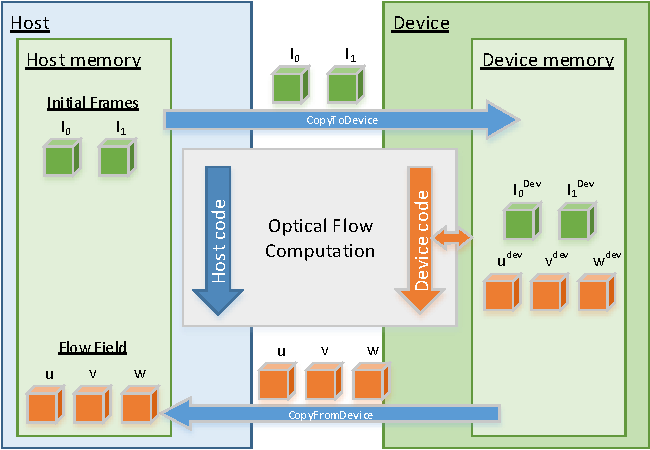
\includegraphics[width=.65\textwidth]{figures/data-copy.pdf}
	\caption{Data transfer between the host and the device for the GPU based implementation of the 3D optical flow algorithm. Image: \cite{KarlinskiyThesis}.}
	\label{fig:data-copy}
\end{figure}

Then, we can estimate the maximum size of the input frame which is possible to process using full GPU version: 
\begin{equation}
15 \times pitch \times height \times depth \times sizeof(float) \leq N.
\end{equation}  
As an example, if we have a GPU with 4GB of memory, we can process input volumes of approximately 273MB, which corresponds to a volume with the sizes about $400 \times 400 \times 400$ voxels.
Obviously, such data sizes are not adequate, if we consider the processing of high-resolution datasets. For large datasets it is then necessary to downsample the initial data, which could lead to a significant loss in resolution and accuracy. To overcome this limitation and enable the processing of large datasets in the next section we present an extension of our GPU implementation.

\subsubsection{Extension for large datasets}

In this section we show how the 3D optical flow method can be extended to support large datasets.
The main idea of the proposed method is to implement the so-called \textit{data partitioning strategy}. We store the dataset and corresponding vector fields in the host memory and transfer smaller portions to the device for parallel processing on GPU. In this strategy, the host performs managing of the data partitioning, execution on the device and collection of the results after each computation level. To perform data partitioning we make the slicing of the original volumes and extend each data chunk with overlapping regions, solve the data dependency problem.   
An example of such partitioning (slicing along Z-axis) is presented in Figure \ref{fig:slicing-overlap}.

\begin{figure}[h]
	\centering
	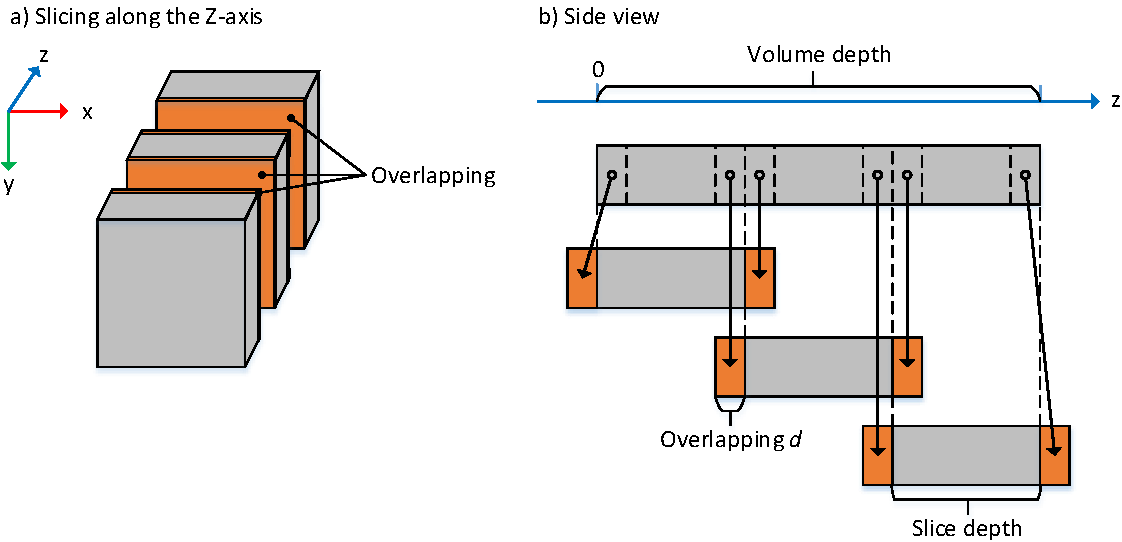
\includegraphics[width=0.8\textwidth]{figures/slicing-overlap.pdf}
	\caption{Data partitioning strategy. Slicing is done along the Z-axis with the overlapping regions (a). Partitioning of voxels in the full volume with overlapping regions (b). The overlapping regions that are outside the full volume are filled with "mirrored" values. Image: \cite{KarlinskiyThesis}.}
	\label{fig:slicing-overlap}
\end{figure}

Note, that in the previous implementation (\textit{full} GPU version) the whole dataset, the resulting vector fields and all auxiliary containers reside in the GPU memory and there is only one data transfer operation from the host to the GPU. In our \textit{extended} version data is transferred between the host and the device before and after processing of each data chunk. Therefore, data transfer can lead to serious performance issues and the bandwidth between the host and the device become a limiting factor. In the next section we provide quantitative performance analysis between CPU and GPU versions, as well as between \textit{full} and \textit{extended} GPU versions.


\subsubsection{Performance evaluation}

To measure the performance of our GPU based 3D optical flow implementation we run the method on datasets with different sizes. Instead of evaluating each individual component of the algorithm, we present the execution time and memory consumption for the whole computation pipeline. Moreover, we verify the correctness of the algorithms compared with the original CPU implementation.   

For the evaluation we use the computation hardware with the specifications presented in Table \ref{tbl:test-machines}.

\begin{table}[h] \scriptsize
	\centering
	\begin{tabular}{l c c}
		\hline
		& CPU Test machine           & GPU Test machine                                                                                  \\
		
		\hline
		CPU        & Intel Xeon Processor X5675 & Intel Xeon Processor E5-2637 v2                                                                   \\
		RAM        & 96 GB                      & 64 GB                                                                                             \\
		GPU        & ---                        & GeForce GTX 980 Ti
		 \\
		GPU Memory & ---                        & 6 GB                                                                                              \\
		CUDA Cores & ---                        & 2816                                                                                             
	\end{tabular}
	\caption{Technical specifications of computation machines used for the performance evaluation.}
	\label{tbl:test-machines}
\end{table}

We estimate how the size of the input data influences performance of 3D optical flow method and the memory consumption by the computation routines. For the evaluation we use  datasets with the following sizes: $100^3$, $200^3$, $400^3$, $600^3$, $800^3$. As it was highlighted previously for a GPU device with 4GB of memory the maximum size of the input data is $400^3$. Therefore, datasets with sizes $100^3$, $200^3$ and $400^3$ can be processed using \textit{full} GPU method; while larger dataset - $600^3$, $800^3$, can be processed only using an \textit{extended} version. 
Evaluation results for performance measurements and memory consumption are presented in Tables \ref{tb:perf-time} and \ref{tb:perf-mem} respectively.

\begin{table}[h] \footnotesize
	\centerline{
		\begin{tabular}{c|c|c|c|cc}
			\multirow{2}{*}{\begin{tabular}[c]{@{}c@{}}Size\\ (voxels)\end{tabular}} & \multicolumn{3}{c|}{\begin{tabular}[c]{@{}c@{}}Execution time\\ (hh:mm:ss)\end{tabular}}                                                                              & \multicolumn{2}{c}{\begin{tabular}[c]{@{}c@{}}Speedup\\ relative to CPU verion\end{tabular}}                                                     \\ \cline{2-6} 
			& \begin{tabular}[c]{@{}c@{}}GPU\\ \textit{Full} version\end{tabular} & \begin{tabular}[c]{@{}c@{}}GPU\\ \textit{Extended} vesion\end{tabular} & \begin{tabular}[c]{@{}c@{}}CPU\\ Version\end{tabular} & \multicolumn{1}{c|}{\begin{tabular}[c]{@{}c@{}}GPU\\ \textit{Full} version\end{tabular}} & \begin{tabular}[c]{@{}c@{}}GPU\\ \textit{Extended} version\end{tabular} \\ \hline
			$100^3$                                                                                 & 00:00:01                                                   & 00:00:13                                                      & 00:00:38                                              & \multicolumn{1}{c|}{41.8}                                                        & 2.9                                                            \\
			$200^3$                                                                                 & 00:00:03                                                   & 00:00:42                                                      & 00:06:02                                              & \multicolumn{1}{c|}{112.4}                                                       & 8.6                                                            \\
			$400^3$                                                                                 & 00:00:19                                                   & 00:03:52                                                      & 01:13:52                                              & \multicolumn{1}{c|}{\textbf{239.4}}                                                       & \textbf{19.1}                                                           \\
			$600^3$                                                                                 & ---                                                        & 00:11:48                                                      & 02:47:53                                              & \multicolumn{1}{c|}{---}                                                        & 14.2                                                            \\
			$800^3$                                                                                 & ---                                                        & 00:26:33                                                      & 07:30:49                                              & \multicolumn{1}{c|}{---}                                                        & 17                                                           
		\end{tabular}
	}
	\caption{Evaluation of execution time for dataset with different sizes $100^3$, $200^3$, $400^3$, $600^3$, $800^3$.}
	\label{tb:perf-time}
\end{table}

\begin{table}[h] \footnotesize
	\centering
	\begin{tabular}{c|c|c|cc}
		\multirow{2}{*}{\begin{tabular}[c]{@{}c@{}}Size\\ (voxels)\end{tabular}} & \multicolumn{2}{c|}{\begin{tabular}[c]{@{}c@{}}GPU\\ \textit{Full} version\end{tabular}} & \multicolumn{2}{c}{\begin{tabular}[c]{@{}c@{}}GPU\\ \textit{Extended} version\end{tabular}} \\ \cline{2-5} 
		& Device memory                          & System memory                          & \multicolumn{1}{c|}{Device memory}                 & System memory                 \\ \hline
		$100^3$                                                                                 & 73 MB                                  & 19 MB                                  & \multicolumn{1}{c|}{*}                           & 57 MB                         \\
		$200^3$                                                                                 & 586 MB                                 & 153 MB                                 & \multicolumn{1}{c|}{*}                           & 458 MB                        \\
		$400^3$                                                                                 & 3.64 GB                                & 1.19 GB                                & \multicolumn{1}{c|}{*}                           & 3.58 GB                       \\
		$600^3$                                                                                 & ---                                    & ---                                    & \multicolumn{1}{c|}{*}                           & 12.07 GB                      \\
		$800^3$                                                                                 & ---                                    & ---                                    & \multicolumn{1}{c|}{*}                           & 28.61 GB                     
	\end{tabular}
	\caption{Memory usage of the implemented framework. Note that the memory allocated on the device is padded to satisfy alignment requirements. (*) For the extended version the usage of the device memory is determined by the current needs for the sliced data and available GPU memory.}
	\label{tb:perf-mem}	
\end{table}

From time measurements we see the following results - for small datasets $\le 400^3$), \textit{full} GPU implementation gives the best performance. Clearly, the \textit{extended} version provides less performance compared to the \textit{full} version due to data transfer operations between the host and the device. However, for larger datasets ($> 400^3$), the \textit{full} version is no longer functional, since the data cannot be fitted into the memory of the GPU, so the data partitioning strategy of the \textit{extended} version has to be used. In this case, the \textit{extended} version significantly outperforms the CPU version of the optical flow method. The maximal performance speedup for the \textit{full} version was 33.5, for the \textit{extended} version -- 11.5. Therefore, we conclude that our 3D GPU-based implementation is efficient and provides a significant reduction in the computation time for large 3D datasets.




%--------------------------------------------------------
\section {Visualization}
%--------------------------------------------------------
\label{visualization}

The section gives a brief summary of visualization methods for time-varying data and results of optical flow computation which are available in our data analysis framework. We implement three main visualization methods:
\begin{itemize}
	\item Vectors fields using glyphs visualization 
	
	\item Scalar properties or other metrics using color pseudo-codes.
	
	\item Motion trajectories using track visualization 
\end{itemize} 

In the following part we describe in more details vector fields visualization using vector glyphs and omit the description of other methods. 

%Examples of vector field visualization and scalar field visualization using magnitude are shown in Figure \ref{fig:vis_vec_comp} alongside with the correspond 3D rendering.
%
%\begin{figure*}[t]
%	\centerline{
%		\mbox{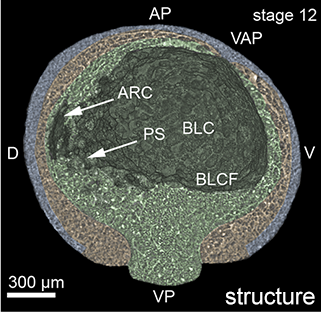
\includegraphics[scale=0.85]{figures/vis_vec_comparison1.png}}
%		\mbox{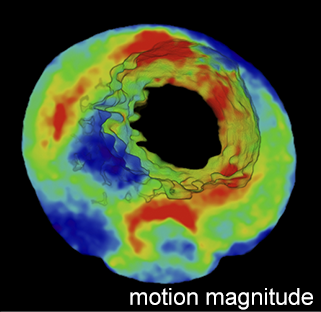
\includegraphics[scale=0.85]{figures/vis_vec_comparison2.png}}
%	}
%	\caption[]{\textbf{Left:} 3D rendering of a halved embryo. \textbf{Right:} 3D rendering of a scalar field representing velocity magnitude.}
%	\label{fig:vis_vec_comp}
%\end{figure*}


\subsection*{Vector Field}

A simple yet effective method for visualization of vectors fields is a glyphs method. In this case each vector of the displacement field is depicted as a glyph with a certain shape and color. 

For our implementation we use 3D cones. For the coloring of glyphs we use two modes: the first one assigns a color according to the magnitude of a vector and the second mode uses the direction of a vector. Both visualization using different coloring schemes are presented in Figure \ref{fig:vec_vis}.

\newcommand{\imageSizex}{0.29}

\begin{figure}[ht]
	\centerline{	
		\mbox{\includegraphicslabeledb[scale=\imageSizex]{figures/magnitude.png}{a}}	
		\mbox{\includegraphicslabeledb[scale=\imageSizex]{figures/direction.png}{b}}
	}	
	\centerline{	
			\mbox{\includegraphicslabeledb[scale=\imageSizex]{figures/threshold-1.png}{c}}	
			\mbox{\includegraphicslabeledb[scale=\imageSizex]{figures/threshold-0.png}{d}}
    }    	
   	\centerline{	
   		\mbox{\includegraphicslabeledb[scale=\imageSizex]{figures/regular.png}{e}}	
   		\mbox{\includegraphicslabeledb[scale=\imageSizex]{figures/jittered.png}{f}}
   	}
		
	\caption{Visualization of a 3D vector field. \textbf{(a)} Using magnitude of the vectors for coloring.  \textbf{(b)}  Using direction of the vectors for coloring.  \textbf{(c)} Regular grid, no threshold of magnitude value. \textbf{(d)} Regular grid, threshold is applied. \textbf{(e)} Regular grid, decreased number of grid points. \textbf{(f)} Jittered grid. Image adopted from: \cite{KarlinskiyThesis}.}
	\label{fig:vec_vis}
\end{figure}

In order to improve the usability of the 3D visualization tool we provide visualization parameters that can be changed interactively. It is possible to adjust the sample grid $G_x$, $G_y$, $G_z$, the glyphs scaling factor and the magnitude threshold. All different visualization modes are presented in Figure \ref{fig:vec_vis}. Moreover, it is possible to use the so-called \textit{jittered} grid. It allows to avoid possible artifacts associated with the regular grid (artifacts similar to aliasing, when viewed from different angles). This improves the clarity of user’s perception of different parts of the vector field. Comparison between a regular and a jittered grid is given in Figure \ref{fig:vec_vis}. All the visualization parameters can be adjusted interactively and the changes are immediately rendered.




%\begin{figure}[h]
%	\centerline{
%		\mbox{\includegraphicslabeledb[scale=0.27]{figures/threshold-1.png}{a}}
%		\mbox{\includegraphicslabeledb[scale=0.27]{figures/threshold-0.png}{b}}
%	}
%	\caption{Different visualization modes. \textbf{(a)} Regular grid, no threshold of magnitude value. \textbf{(b)} Regular grid, threshold is applied. Image: \cite{KarlinskiyThesis}.}
%	\label{fig:vis_modes}
%\end{figure}

%\begin{figure}[h]
%	\centerline{
%		\mbox{\includegraphicslabeledb[scale=0.27]{figures/regular.png}{a}}
%		\mbox{\includegraphicslabeledb[scale=0.27]{figures/jittered.png}{b}}
%	}
%	\caption{Different visualization modes. \textbf{(a)} Regular grid, decreased number of grid points. \textbf{(b)} Jittered grid. Image: \cite{KarlinskiyThesis}.}
%	\label{fig:vis_modes2}
%\end{figure}

For the implementation of our visualization tool we use OpenGL\footnote{\url{https://www.opengl.org/}} as a 3D graphics library, GLFW\footnote{\url{http://www.glfw.org/}} as a library for window and input management, GLM\footnote{\url{http://glm.g-truc.net/}} as a mathematics library for graphics software and AntTweakBar\footnote{\url{http://anttweakbar.sourceforge.net/}} as a light graphical user interface library. All the libraries are cross-platform and free to use.

        
%\subsection{Scalar Field}
%For visualization of scalar fields (see the whole list of metrics in Sections \ref{components_results} and \ref{component_motion}) in 2D or 3D we use a number of look-up tables (LUTs).
%\todo{change: From. Russ.}\change{The use of color scales as a substitute for brightness values allows us to show and see small
%changes locally, and identify the same brightness values globally in an image. This should be
%a great benefit, since these are among the goals for imaging discussed below. Color might be used  to encode flow components, velocity, differently moving objects and other quantitative.
%These uses generally have little to do with the properties of the image and simply take advantage
%of the human ability to distinguish more colors than grey scale values.}
%For visualization of scaler fields we use external software such as ImageJ / Fiji.
%An example of color coding using different LUTs is given in Figure \ref{fig:lookup_tables}.
%
%\begin{figure*}[!ht]
%  \centerline{
%    \mbox{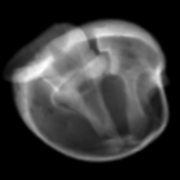
\includegraphics[scale= 0.6]{figures/lut_screw_grey.png}}
%    \mbox{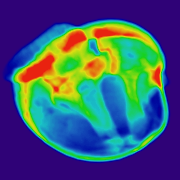
\includegraphics[scale= 0.6]{figures/lut_screw_physics.png}}
%    \mbox{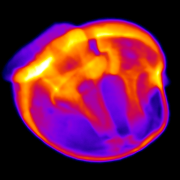
\includegraphics[scale= 0.6]{figures/lut_screw_fire.png}}
%  } 
%  \vspace{3pt}
%   \centerline{
%    	\mbox{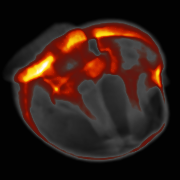
\includegraphics[scale= 0.6]{figures/lut_screw_smart.png}}
%    	\mbox{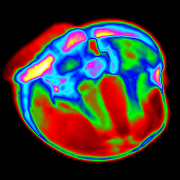
\includegraphics[scale= 0.6]{figures/lut_screw_6_shades.png}}
%    	\mbox{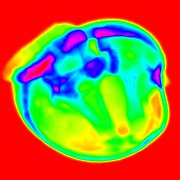
\includegraphics[scale= 0.6]{figures/lut_screw_spectrum.png}}
%    }
%
%  \caption[Noise filterst]{Color coding of a projection radiograph using different color-codes. Note that different local and global image features are highlighted by each look-up table.}
%  \label{fig:lookup_tables}
%\end{figure*}




%\subsection{Line Convolution}
%
%[pages 0.5-1]
%
%\begin{itemize}
%	\item Name
%  \item Description, Shows what?
%  \item Example image
%  \item Best usage examples
%\end{itemize}

%\subsection{Tracks}
%
%Visualization of tracking information is implemented using external software packages such as Amira/Avizo software\footnote{\url{http://www.fei.com/}} and Paraview\footnote{\url{http://www.paraview.org/}}.
%Our computational framework outputs the tracking information in formats, recognizable by these software packages. Few examples of tracks visualization using Avizo software are presented in Figure \ref{fig:vis_vec_comp}. 
%	 
%
%\begin{figure*}[!ht]
%	\centerline{
%		\mbox{\includegraphicslabeledw[scale=0.35]{figures/vis_tracks_random.png}{a}}
%		\mbox{\includegraphicslabeledw[scale=0.35]{figures/vis_tracks_arch.png}{b}}
%	}
%	\caption[]{\todo{Extend description}Visualization example of tracking information.  \textbf{(a)} Short tracks of cells distributed on a regular grid. The color denotes time. \textbf{(b)} Tracking of morphological changes in internal structures. \change{Colors correspond to outlines of different organs.}}
%	\label{fig:vis_vec_comp}
%\end{figure*}





%\subsection{Color Coding}
%
%Link: http://hci.iwr.uni-heidelberg.de/Static/correspondenceVisualization/
%
%To show:
%\begin{itemize}
%	\item 2D Bruhn colors
%	\item 2D Middl colors
%  	\item 3D RGB cube
%  	\item 3D projections: XY, YZ, XZ
%  	\item Simplified colors: 6, more
%\end{itemize}








%******************************************************************
%******************************************************************
\chapter {Evaluation on Synthetic Data}
\label{experiments}
%******************************************************************
%******************************************************************

In this chapter we perform  systematic experiments on synthetic data, designed to test the performance of optical flow methods.  In the beginning of the chapter we provide a taxonomy of X-ray data. Our classification includes evaluation of image quality, description of data features and artifacts, as well as the description of motion models. Then, we present synthetic datasets, which we employ for our experimental evaluation. Further, we discuss an important aspect of parameters optimization and describe the overall quantitative evaluation procedure.  We present a discussion on the performance, influence of preprocessing, modelling of noise and data outliers and the use of confidence measures. For all the experiments we outline important observations and draw the conclusions, which we summarize in the end of the chapter.


%--------------------------------------------------------
\section{Data Taxonomy}
%--------------------------------------------------------
\label{data_taxonomy}


Since correspondence problems are highly ill-posed and challenging to solve, before any data processing steps are performed, the input data should be systematically evaluated. Its quality, description of the moving objects or the scene, and the motion model should provided a basis for the choice of appropriate data preprocessing routines and optical flow models. Moreover, we emphasize that the clear definition of the application and description of the requirements on the algorithm should be specified. 

One approach to evaluate the data is to perform an explicit quantitative description of the input images. For example, compute a histograms of grey values and velocities, provide the distribution of image derivatives, use noise estimators, etc.
But, it is not always possible to provide such an extensive description - noise estimation can be a difficult task, the motion model prior to the optical flow computation is not known, artifacts are difficult to estimate. In our case we aim to provide a systematic, yet simple and consistent data classification model, which is handy to apply for a wide range of datasets and applications.

In the rest of this section we enlist the most important aspects for our data taxonomy classification. The first category is a description of the image quality.





\subsection{Image Quality}
\textbf{Image Noise}
\\
\\
Noise is a fundamental characteristic of image data. The presence of noise affects the image quality and deteriorates data analysis. To describe the image noise we consider two parameters - the noise model and the amount of noise (or noise level).
\\
\\
\textit{Noise Model}. Is an important characteristic, since it determines the choice of filtering procedure and impose certain requirements on the design of optical flow models. Various noise models that are important for our work are described in Section \ref{noise_models}. 
For our data taxonomy we distinguish the following noise models:
\begin{itemize}
	\item Gaussian noise. This noise model is an approximation model and is frequently used for synthetic datasets in a large body of work on optical flow methods. However, as we have discussed earlier, this model does not adequately describe a physical process of imaging, especially X-ray imaging. 
	
	\item Poisson noise. That is the most important source of noise for X-ray images due to the photon statistics and the detection process. Therefore, it is crucial to test the performance of optical flow methods and the processing techniques on the type of noise.
	
	\item Spike noise. An important noise model to evaluate the performance of computational methods with respect to data outliers.
	
	\item Granular noise. This type of noise is characterized by the varying size and the unknown distribution function. The presence of such noise can be a result of a preprocessing routine, e.g. tomographic reconstruction.
\end{itemize}
Examples of images contaminated with different noise are shown in Figure \ref{fig:noise_models}.
%\comment{Put away this? dont need to give solutions here}To cope with noisy image data two strategies or a combination of them can be employed: use preprocessing step and filter noise from the image data and then proceed with data analysis; use original noisy data as an input for a robust optical flow model. In Section \ref{} we described possible noise filtering methods and in experimental section(s) \ref{}, \ref{} made quantitative evaluation of these techniques.  Based on these experiments we can make the following conclusions: if the amount of noise is small - already a second strategy, i.e. robust optical flow model, can provide good results, otherwise, for high amount of noise - a careful preprocessing step, followed by a robust optical flow computation should be used.
\\
\begin{figure*}[ht]
	
	\centerline{
		\mbox{\includegraphicslabeledw[scale=0.38]{figures/noise_example_poisson.png}{a}}
		\mbox{\includegraphicslabeledw[scale=0.38]{figures/noise_example_spike.png}{b}}
		\mbox{\includegraphicslabeledw[scale=0.38]{figures/noise_example_granular.png}{c}}
	} 
	\caption[]{Examples of X-ray images containing different types of noise. \textbf{(a)} Radiographic image with a large amount of the Poisson noise, as a result of a short exposure time. \textbf{(b)} X-ray image with a good signal-to-noise ratio, but with a substantial amount of the Spike noise (saturated pixels). \textbf{(c)} Radiographic image with the granular noise resulting from a post-processing step of the raw data.}
	\label{fig:noise_models}
\end{figure*}

\textit{Noise Level}. This parameter specifies the amount of noise. As it was already mentioned in the previous section, adequate quantitative estimation of a noise level is a challenging task. Even when such procedure is feasible to perform, it is not clear how to employ this quantitative information to guide the design of processing procedures. For this reason, we omit a measurable estimation of a noise level and proceed with a qualitative, empirical estimation approach. For this purpose we distinguish the following noise levels: 
\begin{itemize}
	\item low: no noise or very little noise is present. In this case no special data treatment is required and design choices for the optical flow model are not restricted to methods that are robust with respect to noise.  
	
	\item average: there is a considerable amount of noise, but the image features are well discernible. A careful consideration of noise is required.
	
	\item high: image data is highly deteriorated with noise. An advanced noise filtering and robust optical flow methods are mandatory to obtain reliable optical flow results.
\end{itemize}

\vspace{0.4cm}
\textbf{Image Contrast}
\\
\\
We refer to the image contrast, as a general ability to distinguish between different image structures. As we already pointed out in Section \ref{contrast_estimation} the contrast-to-noise ratio (CNR) is a more descriptive and useful measure to evaluate the contrast and its implications on the data analysis, then the signal-to-noise ratio or solely image contrast measures.

In the same manner as for the classification of an image noise, we distinguish three contrast levels:
\begin{itemize}
	\item high: there is a pronounced difference in contrast of image features. This includes a high amount of textures and regions with large values of image gradients. This type of datasets is preferred for the  data analysis and usually leads to an accurate optical flow results.
	
	\item average: a contrast is enough to clearly distinguish between features of interest. Moreover, a signal-to-noise ratio for the dataset is acceptable.
	
	\item low: different image features can be hardly distinguished. Additionally, a signal-to-noise ratio is poor, which makes it difficult to enhance the contrast (e.g. using histogram stretching) without augmenting the noisy part of a signal. This case is one of the most challenging image analysis scenarios and an advanced data preprocessing procedure is mandatory to retrieve useful information. 
	 
	  
	
\end{itemize}

Examples of different contrast levels are shown in Figure \ref{fig:contrast_level_examples}.

\begin{figure*}[ht]
	
	\centerline{
		\mbox{\includegraphicslabeledw[scale=0.38]{figures/contrast_example_high.png}{a}}
		\mbox{\includegraphicslabeledw[scale=0.38]{figures/contrast_example_normal.png}{b}}
		\mbox{\includegraphicslabeledw[scale=0.38]{figures/contrast_example_low.png}{c}}
	} 
	\caption[]{Examples of X-ray images with different contrast levels. \textbf{(a)} Radiographic image of aqueous foam with high contrast and good signal-to-noise ratio. \textbf{(b)} Tomographic 2D slice through a \textit{Sitophilus granarius} beetle. The dataset has relatively low contrast between internal structures and poor SNR. \textbf{(c)} Radiographic image of a semi-liquid alloy. Contrast between liquid phase (bright part) and metal particles (dark spots) is very low. Moreover, SNR ratio  is very low.}
	\label{fig:contrast_level_examples}
\end{figure*}

\subsection{Data Features}


%pale green 	#98FB98 	(152,251,152)
%light coral 	#F08080 	(240,128,128)
%lemon chiffon 	#FFFACD 	(255,250,205)


%
%\begin{tabular}{l|c|r}
%  \hline
%  \cellcolor{good}Some & \cellcolor{norm}coloured & \cellcolor{bad}bad \\
%  \hline
%\end{tabular}
%\end{document}


In this section of our data taxonomy we provide a set of parameters to describe a visual appearance of the scene and its objects. Depending on the visual and morphological characteristics of moving objects, different types of optical flow models and their parameters might be optimal. 
In general, all the information about the scene should be identified and described in details. First, this imposes constraints on data constancy assumptions. Second, it describes the requirements for the flow field. Finally, it states the task for the optical flow computation - for which parts of the scene, which dynamical information should be computed. 

Here we list the main aspects of the description of a scene and its objects, that are used in our data classification:
\\
\\
\textit{Object size}.  One of the basic characteristics of an object is its size. The distribution of object sizes may vary a lot within a given dataset. For our classification we are interested to describe extreme values of object sizes, i.e. small and large objects. Additionally, it is important to identify cases, when both categories of objects are present within the same scene.   
Thus, we may distinguish the following categories of object sizes:
\begin{itemize}
	\item small: if the objects of interest are small, a special care should be taken when choosing computational methods and their parameters. For example, if we aim to compute the optical flow on small features, the size of a median mask (See Section \ref{flow_median}) should be adjusted accordingly, since it might eliminate the flow around such small features. In a similar way, the large flow regularization parameters may lead to an oversmoothing of the flow field, resulting in a loss of flow details for small objects.
	
	\item average: by an average size we assume a range of sizes, which do not belong to the extreme values of our categorization approach. In general, such kind of objects do not introduce any restrictions on optical flow models.   
	
	\item large: by a large object we define the object which size exceeds 10-20\% of an image size. In general, the computation of optical flow on large objects should not differ from the objects of average sizes. However, there is an exception. If the object is homogeneous (i.e. contains a small amount of details) and the task is to capture a dense flow field within this object, a large value of the smoothness parameter is required. This can affect the computation in other image regions that contain different data features. That is why the presence of large homogeneous objects should be noted. 
	
	\item mixed: for this case we consider a mixture of small and large objects. This situation is the most challenging, since it requires the simultaneous optimization of parameters for all objects sizes. It is a common problem in the literature that the small image features get smudged because of a significant contribution from the smoothness term. One way to deal with this problem is to use an adaptive smoothness (See Section \ref{adaptive_smoothness}) in different image regions. Another solution is a fusion of results obtained using different model parameters that are specifically tuned for each object category. In any case, a mixture of different objects sizes introduces a major problem for the optical flow computation.   
\end{itemize}

\noindent \textit{Object distribution}. A spatial relationship between objects, i.e. objects density. To describe the object distribution we use the following cases:
\begin{itemize}
	\item sparse: in this situation the objects are distant from each other, separated by a homogeneous background.  Despite the fact that this situation might seem to be easy to handle by optical flow methods, there are some pitfalls. The problem arises from the homogeneous background which separates the objects. In this region there is no contribution from the data term, i.e. aperture problem exists (See Section \ref{general_model}), so the smoothness term takes a lead. As a result, on the boundary between an  object and a background the oversmoothing problem might occur (which depends on the chosen parameter for the flow regularization $\alpha$). And if the object of interest also appears to be details-free, even a larger value of the smoothness parameter is required to precisely capture the motion within such object. In this situation severe oversmoothing artifacts may occur. To summarize, a sparse object distribution can be troublesome in conjunction with the low amount of object details (See next characteristic of object features).
	
	\item normal: this case describes a normal situation for object distribution. Objects might be close to each other or even share a common boundary, but the length of this interface is much smaller, then the perimeter of the corresponding objects. 
	
	\item dense: the objects are close to each other and share substantial amount of their boundaries with other objects. Clearly, in this case a special attention should be paid when choosing optical flow parameters that might lead to imprecise localization of object boundaries. Such parameters include, the gradient constancy assumption as a data term, the presmoothin parameter $\sigma$, the flow regularization parameter $\alpha$, the integration scale $\rho$ and the mask size for the flow median filtering.  
\end{itemize}


\noindent \textit{Object details}. This characteristic describes the amount of image features or details  for the objects of a scene. We distinguish the following quantities of object details:  
\begin{itemize}
	\item low: small amount or no image details (homogeneous objects). For such objects the optical flow computation may be a challenging task and the inappropriate choice of the regularization parameter may lead to oversmoothness artifacts. 
	
	\item normal: this case describes an ideal situation. It means that the amount of image gradients is sufficient to provide enough contribution to the data term. So, no aperture problem exists in most image regions.
	
	\item high: in general, the more details an object has, the more information is available for the data term. However, there might be some exceptions. For example, in \cite{HarmonyFlow} the authors found out that repeating high-frequency image texture can cause aliasing artifacts during the resampling procedure. As a result, the accuracy of optical flow estimation in these regions can be substantially impaired.  Thus, it is important to describe such high-frequency textures and any other periodic structures beforehand.
\end{itemize}


\subsection{Image Artifacts}
\label{image_artifacts}

In this section we present a description of various image artifacts, which affect results of data analysis. All artifacts, if existing, should be treated by an appropriate processing step or computed using a dedicated optical flow model. 
Here we provide a list of possible image artifacts:
\begin{itemize}
	\item \textit{Brightness variations}. Brightness of X-ray images can be non-uniform spatially and non-constant over time (See Figure \ref{fig:artifacts_examples}). Since the main component of every optical flow model is a data term, which imposes certain constancy assumptions on image brightness or other image-based features, the presence of brightness variations is crucial for the design of optical flow models.  
	
	\item \textit{Ring artifacts}. Damaged elements of a detector system cause individual pixels to remain constant during an image acquisition and in particular during the tomographic scanning process. As a result, line structures on sinograms appear. After the reconstruction is performed using the filtered backprojection algorithm these lines form the so-called ring artifacts (See Figure \ref{fig:artifacts_examples}). Such artifacts can significantly deteriorate the accuracy of data analysis. Thus, such artifacts should be removed prior to motion estimation.
	
	\item \textit{Star artifacts}. A non-linear relation between the attenuation coefficient in the material and the intensity values measured by the detector system give rise to the so-called beam-hardening artifacts. These artifacts appear along a geometric path of the respective X-ray beam. After the reconstruction such artefacts appear radially around the boundaries of on object and are called star artifacts (See Figure \ref{fig:artifacts_examples}). Usually, such artifacts are not so pronounced in the region within an object, however, can lead to the incorrect flow estimation on the boundaries of an object. As a possible remedy one can use a dedicated image reconstruction procedure, which is more robust to the beam-hardening artifacts, i.e. algebraic reconstruction techniques with a spatial image regularisation. 
	
	\item \textit{Motion blur}. For the conventional reconstruction methods such as the filtered-back projection, it is assumed that the object is not changing during the acquisition process, so one obtains radiographic projections of the same object from multiple angles. But, this assumption is not always fulfilled. This could be a result of sample motion due to poor experimental conditions, e.g. bad fixation of the sample. Additionally, the motion of a sample could be a part of the experiment, which aims to study dynamical processes. In any case, the inconsistent projection data will result in motion artifacts in the reconstructed volume. The amount of motion blur and the specific steps to take it into account should be described prior to the actual flow computation. 
	
	\item \textit{Projective geometry}. This kind of artifact is characteristic to the radiographic imaging where 3D structures are projected into a 2D detector plane. This effect is similar to the problem of occlusions in the classical optical flow. Such artifacts are non-existing for tomographic data, in which a 3D information about the scene is available. Projective geometry poses a major problem for optical flow computation, since it deteriorates the data constancy assumption.
\end{itemize}

For our data taxonomy, if any of the above mentioned artifacts exists, we mark it as a possible data challenge and provide a list of steps to compensate for it.

%Possible sources of brightness variations:
%\begin{itemize}
%	\item Monochromator stripes (variations)
%	\item Exposure changes
%	\item Changes in sample environment (background)
%	
%\end{itemize}

A list of examples of various image artifacts is shown in Figure \ref{fig:artifacts_examples}

\begin{figure*}[ht]
	
	\centerline{
		\mbox{\includegraphicslabeledw[scale=0.38]{figures/artifacts_examples_bright.png}{a}}
		\mbox{\includegraphicslabeledw[scale=0.38]{figures/artifacts_examples_rings.png}{b}}
		\mbox{\includegraphicslabeledw[scale=0.38]{figures/artifacts_examples_stars.png}{c}}
	} 
	\caption[]{Examples of X-ray images with various image artifacts. \textbf{(a)} Radiographic image of living embryo. Non-uniform brightness variations due to monochromator instabilities. \textbf{(b)} Tomographic 2D slice through a \textit{Xenopus leavis} embryo. Ring artifacts are highly pronounced and severely degrade the image data. \textbf{(c)} Tomographic 2D slice through a weevil incorporated in amber. Note star artifacts due to the beam hardening.}
	\label{fig:artifacts_examples}
\end{figure*}




\subsection{Motion Model}

In order to compute motion one needs to describe which transformations the objects of a scene undergo. In this section we list data properties, which are related to the motion model. We distinguish the following characteristics:
\\
\\
\textit{Motion model}. In general, a motion field is a vector-valued function of spatial coordinates. For practical reasons, it is useful to describe a motion field by means of a simplified model with fewer parameters. The most important motion models for our work are:
\begin{itemize}
	\item translation: the simplest motion model described by a single displacement vector. This transformation preserves the orientation of an object. In most cases this motion model do not pose troubles for the computation of the optical flow.
	\item rotation: is described by the axis of rotation and the angle of rotation. An important aspect of this transformation is that not all data constancy assumptions are invariant under it. For example, gradient constancy assumption, which contains directional information \ref{data_constancy_assumptions}. Clearly, this aspect should be taken into account for the selection of data term.
	\item rigid (translation + rotation): this transformation corresponds to the standard motion model of a rigid body. 
	\item non-rigid: this transformation is not represented by a parametric motion model. Instead, the motion assumed to be local with a certain constraint on its  smoothness (e.g. elastic transformation) or unconstrained at all. 
\end{itemize}

%A summary of 2D transformation is presented in Figure \ref{fig:motion_models} \cite{Szeliski06}.

%\begin{figure*}[ht]
%	
%	\centerline{
%		\mbox{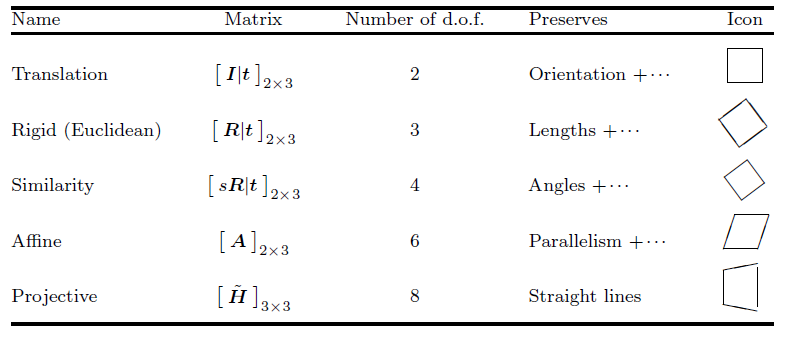
\includegraphics[scale=0.5]{figures/motion_models.png}}
%	} 
%	\caption[]{Hierarchy of 2D coordinate transformations. Image source \cite{Szeliski06}.}
%	\label{fig:motion_models}
%\end{figure*}

\noindent \textit{Motion range}. Another important measure to describe the motion model is to specify the range of velocities with which the objects of the scene move. We distinguish the following motion rates:
\begin{itemize}
	\item small displacement: typically in the range of 1-2 pixels. In this case the linearization of the data term can be performed via the first-order Taylor expansion leading to a convex formulation of the optical flow problem (See Section \ref{general_model}). 
	
	\item large displacement: as soon as large values of object displacements are assumed, we cannot employ linear data terms. This is why an appropriate computation strategy have to be used (See Section \ref{multilevel}). Also the optimal size for the coarsest resolution level is an important factor (See Section \ref{opt_warping_scale}).  
	
	\item mixed: a scenario when both small and large displacements are present and are of interest for the data analysis. For this case, the influence of the  smoothness term should be carefully controlled to preserve small displacements, which tend to be smeared out in the vicinity of a fast motion.
	Additionally, one may consider the adaptive smoothness approach (See Section \ref{adaptive_smoothness}) or a more sophisticated model to respect small movements.
\end{itemize}


\noindent \textit{Motion discontinuities}. It is important to describe the amount of motion discontinuities within a scene. This characteristics plays a key role for the choice of the smoothness constraint. Both spatial and temporal discontinuities should be reported. The following scenarios are important for our data taxonomy:
\begin{itemize}
	\item no discontinuities: for this case we assume a global motion of a scene, described by the same motion model.
	
	\item normal amount: this situation corresponds to a normal case of optical flow computation. There are always discontinuities between objects which are moving with different velocities or directions. Moreover, there is always a motion boundary between the moving object and the static background. It is important to note, that the smoothness assumption is always violated to some extent. The only aim of preserving discontinuities via the appropriate choice of a smoothness term is to allow for piecewise-smooth motion fields.
	
	\item large amount: the cause of discontinuities is the same. i.e. the differences in motion fields, but the amount of flow gradients is large, which requests a particular attention for the choice of a smoothness approach and the corresponding parameters.   
	 
	\item occlusions: in the literature on optical flow methods occlusions between objects or their parts is a major problem. As a result, in the occluded regions not only the information for the data term is lost, but also strong motion discontinuities occur. For X-ray imaging applications occlusions are not present for tomographic datasets, since a 3D information about objects is available. The case when the occlusion problem displays itself is a radiography method, where the projection of 3D structures into a 2D plane gives similar effects. Another important case is the appearance or disappearance of information. This might be a new object entering the scene or formation of a crack in a material, or the process of cell division. For these cases both the data constancy and the motion consistency assumptions are violated.              
\end{itemize}



%--------------------------------------------------------
\subsection{Results Characterization}
%--------------------------------------------------------

To complete our data taxonomy we introduce another important topic - characterization, or requirements, for the output of the  optical flow.
At this point we consider the following important aspects:
\\
\\
\noindent \textit{Accuracy}. No real-life optical flow application should be started without defining the requirements for the accuracy of a result. It can be specified as an upper bound for an average or a maximum error using a chosen error metric (e.g. endpoint error). After the flow field is computed, the results have to be evaluated according to the imposed accuracy limits. This can be achieved by the  comparison with a manual tracking, or using automated confidence measures (See Section \ref{confidence_measures}), or by checking the computed flow with the a-priori information (in the case if motion of some objects is known or can be deduced).   
Verification by visual means may also provide some clues about the accuracy of the computed flow field, but cannot be considered as a reliable way to justify the correctness of the results.  Without specification of error limits and subsequent quantitative verification of the result, the computed flow field cannot be conclusive and trustworthy.            
\\
\\
\noindent \textit{Density}. Specifies whether a dense (i.e. available at every pixel) flow field is required or a sparse representation, available at specified locations is sufficient for the given task. 
\begin{itemize}
	\item sparse: in some cases the requirement on the density of a flow field can be relaxed, which can give a certain degree of freedom to choose model parameters and strategies for the post-processing. For example, one can perform the averaging of the flow vectors from multiple locations or make interpolation of the result using points of high fidelity. These approaches can be especially beneficial for the case of challenging datasets.
	
	\item dense: this is the default scenario for the classical optical flow formulation, where the flow vector is computed for every pixel location.
\end{itemize}

\noindent \textit{Motion components}. Describes which feature of the motion field we are interested to compute. If only one component of the motion field is of relevance, this might give some flexibility to optimize model parameters.
\begin{itemize}
	\item magnitude: if one is interested to estimate the amount of motion, the directional information is not very useful. An example of such scenario is the task of computation of a time-to-impact in driver assistance systems.
	
	\item direction: f one is aimed to estimate directional distribution of the motion field. For this case, the magnitude of the flow field is not relevant.
	
	\item full flow: that is the classical formulation of optical flow, when a flow vector, containing both the direction and the magnitude, is required. 
\end{itemize}


\noindent \textit{Consistancy}. This requirement assumes the consistency of the computed flow field in a forward (between the first image and the second) and backward directions. This condition may be important for various tasks such as image registration and video processing. By the consistency we imply that the flow is the same, but opposite in direction.   
\begin{itemize}
	\item forward: the classical formulation of optical flow, which determines the flow field only in a forward direction.
	
	\item consistent: the motion field, computed in a forward and backward directions should be consistent.
\end{itemize}


\noindent \textit{Motion boundaries}. Before starting optical flow computation it is useful to specify how motion boundaries around moving objects should be treated. Again, this property may be different for various applications. 
\begin{itemize}
	\item strict: Accurate recognition of motion discontinuities is required. In this case a spacial attention should be given to the features of a computation model, which may lead to an oversmoothing or a coarsening of the motion boundaries.
	
	\item not strict: Overall (average) flow is more important and requirements on the precise boundaries estimation are relaxed.
\end{itemize}


\noindent \textit{Computation time}. An important requirement for an optical flow method is the time required to perform the computation. This aspect can significantly influence the choice of an optical flow model, its parameters and the overall accuracy. The requirement is governed by a particular application.       
\begin{itemize}
	\item real-time: for some kind of applications such as driver assistant systems the computation time is crucial. That is why the design of optical flow models is restricted to high-performance methods. 
	
	\item interactive: for some applications the real-time performance is not required, however, some feedback from an user is expected. For instance, if the user wants to inspect the computed flow fields and adjust computation parameters. 
	
	\item offline: for this case there are no limitation on the processing time, so the computation is completely offline. It means that the time complexity of an algorithm is not taken into account and the accuracy of a result is the top priority.
\end{itemize}


\noindent \textit{Data size}. Describes the data size of the input and whether it is possible to process using available memory resources and particular implementation. For the optical flow problem at least two image frames and the flow field should be stored in the memory of a computation unit. For more complex methods, such as a multi-level optical flow (See Section \ref{large_displacements}), motion increments and resampled input images should be additionally stored on each computation level. For some datasets, especially this is typical for a large tomographic volumes, the input data and all variables required for an algorithm, do not fit into the available memory. Thus, the input should be reduced (i.e. using downsampling or cropping), leading to a possible loss of resolution and accuracy. 


%--------------------------------------------------------
\section{Experimental Data}
%--------------------------------------------------------

In order to perform a systematic evaluation of different features of optical flow models, test the results of  data preprocessing routines and investigate the influence of image artifacts, we need to have a set of synthetic test data for which a ground truth result is known.
To obtain such datasets for X-ray images one may proceed in two directions: generate synthetic images exclusively for the X-ray data (see our data taxonomy Section \ref{data_taxonomy}) or, alternatively, one may use the existing datasets and model X-ray related image properties, such as image noise, low contrast and artifacts. 
In this work we proceed with the second approach and use synthetic datasets which are popular in the literature on optical flow methods. Our choice is based on a number of advantages, associated with the second approach. First, these datasets are extensively used and many optical flow methods are already evaluated using them, which makes it easy to compare our results with the previous work. Second, these datasets are publicly available, which can increase the reproducibility of the results. 


  

  

\subsection{Synthetic Datasets}
\label{synthetic_data}

Here we describe synthetic datasets, which we choose for our experimental studies. In total we include three datasets: two datasets depicting a real scenery and one synthetic dataset.

First two image sequences were developed and presented in the work of \cite{Middl}.  The authors made an extraordinary effort to obtain a realistic non-rigid scenes for which a highly accurate optical flow result is available.  In this technique a scene is built from real-life objects and each element of the scene is moved using a mechanical motion stage. The authors applied a fine spatter fluorescent pattern to surfaces of all scene objects. Then, the camera recorded a pair of high-resolution images under the ambient light and the UV illumination (which revealed fluorescent particles). 
The ground truth is obtained by tracking small image blocks in the high-resolution UV images to get integer-valued motion correspondences. As a second step the authors refined the ground truth to the sub-pixel precision using the Lukas-Kanade optical flow algorithm \cite{LucasKanade81}. As a result, a dense ground truth with a verified precision of about 1/10 pixel in the original size and 1/60 pixel in the downsampled size (used as the final result) is obtained.

Here we describe the selected datasets according to our data taxonomy (See Section \ref{data_taxonomy}). 
\\
\\
\textit{RubberWhale} dataset. It contains several independently moving objects, various motion types including non-rigid motion and rotation, different amount of textures.  
Evaluation according to our data taxonomy yields:
\begin{itemize}
	\item \textit{Image noise}: There is no noise in this dataset, perfect imaging conditions.
	
	\item \textit{Contrast level}:  The image contrast is high, the  separation between the objects is good.
	
	\item \textit{Object size}: The scene depicts objects of various sizes, but no small objects are present.
	
	\item \textit{Object distribution}: Objects are distributed normally.
	
	\item \textit{Object details}: Images contain objects with different amount of textures - some of them are highly textured and some of them are more homogeneous. In general, all objects have normal or high amount of details.
	
	\item \textit{Image artifacts}: There are no image  artifacts.
	
	\item \textit{Motion type}: Several types of motion, including translation, rotation, non-rigid motion are present within this dynamic scene. Note, that non-rigid movements (on the blanket, see Figure \ref{fig:gt_images}) vary smoothly, so we do not expect it to cause complications for the optical flow estimation.
	
	\item \textit{Motion range}: Objects are moving with the mixed range of velocities, including slow and fast motion.
	
	\item \textit{Motion discontinuities}: There are occlusions between moving objects, but not very strong ones.
\end{itemize}

\begin{figure*}[!t]
  \centerline{
    \mbox{\includegraphicslabeledw[scale=0.35]{figures/rub1.png}{a}}
    \mbox{\includegraphicslabeledw[scale=0.35]{figures/rub_grounfTruth_bruhn_scale_2px.png}{b}}
  }
  
  \vspace{3pt}
  \centerline{
    \mbox{\includegraphicslabeledw[scale=0.35]{figures/hyd1.png}{c}}
    \mbox{\includegraphicslabeledw[scale=0.35]{figures/hyd_groundTruth_bruhn_scale_2px.png}{d}}
  } 
  \vspace{3pt}
   \centerline{
    \mbox{\includegraphicslabeledw[scale=0.4]{figures/new_marble150.png}{e}}
    \mbox{\includegraphicslabeledw[scale=0.4]{figures/marble_groundTruth_bruhn_scale_2px.png}{f}}
  } 
  
  \caption[]{Synthetic datasets used in the scope of this work for quantitative evaluation of optical flow methods and preprocessing routines. \textbf{(a,b)}  \textit{RubberWhale} dataset. \textbf{(c,d)} \hyd dataset. \textbf{(e,f)}  \mar dataset. Left column: First frame of the corresponding image sequence. Right column:  Ground truth motion field using color code.}
  \label{fig:gt_images}
\end{figure*}
A summary of evaluation of the \rub dataset is given in Table \ref{tab:eval_rub}. The corresponding color codes to classify the influence of certain properties of input data according to our data taxonomy are given in Table \ref{tab:color_codes}.

\begin{table}[ht] \footnotesize
	\centering
	\caption{Color codes to classify the influence of certain properties of input data according to our data taxonomy.}
	\begin{tabular}{ccc}
		\toprule
		\textbf{Color} & \textbf{Description}  \\ 
		\midrule
		\cellcolor{good} good     	    & the feature is advantageous for data processing \\
		\cellcolor{norm} normal     	& in general, the feature should not cause problems  \\
		\cellcolor{bad} challenge     	    & the feature presents a significant challenge \\   
		\bottomrule
	\end{tabular}
	\label{tab:color_codes}%
\end{table}

\begin{table}[ht] \footnotesize
\centering
\caption{Evaluation of \rub dataset.}
\begin{tabular}{ccc}
\toprule
\textbf{Image} & \textbf{Data}   & \textbf{Motion}   \\ 
\midrule
\cellcolor{good} noise: no      	    & \cellcolor{good} size:  average/large  		& \cellcolor{norm}type: vary, non-rigid    \\ 
\cellcolor{good} contrast: high  	& \cellcolor{good} dist: norm     	& \cellcolor{norm} range: mixed  \\ 
\cellcolor{good} artifacts: no       & \cellcolor{good}detail: normal / high 	&  \cellcolor{norm} disc: occlusions   \\ 
\bottomrule
\end{tabular}
\label{tab:eval_rub}%
\end{table}



\textit{Hydrangea} dataset. Contains a large, highly-textured object, which rotates with a fast angular velocity in front of a large background. That background undergoes a translational movement.
Evaluation according to our data taxonomy yields:
\begin{itemize}
	\item \textit{Image noise}: There is no noise in these images, perfect imaging conditions.
	
	\item \textit{Contrast level}:  The image contrast is high, the  separation between the object and the background is good.
	
	\item \textit{Object size}: The scene depicts one object of a large size and large background.
	
	\item \textit{Object distribution}: Only one object is moving in front of the background.
	
	\item \textit{Object details}: The object (a plant) contains a lot of details (leaves). Background is highly textured. Individual leaves, however, have not much details.
	
	\item \textit{Image artifacts}: There are no image  artifacts.
	
	\item \textit{Motion type}: Translational motion of the background. Fast rotation of the object. 
	
	\item \textit{Motion range}: Objects are moving with approximately the same velocity range.
	
	\item \textit{Motion discontinuities}: There is a substantial amount of occlusions around and within the rotating object.
\end{itemize}
A summary of evaluation of the \hyd dataset is given in Table \ref{tab:eval_hyd}.
\begin{table}[ht] \footnotesize
\centering
\caption{Evaluation of \hyd dataset.}
\begin{tabular}{ccc}
\toprule
\textbf{Image} & \textbf{Data}   & \textbf{Motion}   \\ 
\midrule
\cellcolor{good} noise: no      	    & \cellcolor{good} size: large  		& \cellcolor{good} type: rigid, rotation   \\ 
\cellcolor{good} contrast: high  	& \cellcolor{good} dist: norm     	& \cellcolor{good} range: small  \\ 
\cellcolor{good} artifacts: no       & \cellcolor{good} detail: normal / high 	&  \cellcolor{bad} disc: flow discontinuities   \\ 
\bottomrule
\end{tabular}
\label{tab:eval_hyd}%
\end{table}
\\
\\
\textit{New Marble} dataset. It is a computer generated synthetic dataset, which contains two marble blocks moving on a marble floor. This sequence is available at  \url{http://i21www.ira.uka.de/image_sequences/}.
Evaluation according to our data taxonomy gives us:
\begin{itemize}
	\item \textit{Image noise}: There is no noise in these images, the scene is synthetically rendered.
	
	\item \textit{Contrast level}:  The image contrast is high.
	
	\item \textit{Object size}: The scene depicts objects of normal size.
	
	\item \textit{Object distribution}: Normal object distribution.
	
	\item \textit{Object details}: Objects and background  contains a lot of details.
	
	\item \textit{Image artifacts}: There are no image  artifacts.
	
	\item \textit{Motion type}: Translational motion of two blocks, static background. 
	
	\item \textit{Motion range}: Objects are moving with similar velocities.
	
	\item \textit{Motion discontinuities}: There are occlusions around moving objects.
\end{itemize}
A summary of evaluation of the \hyd dataset is given in Table \ref{tab:eval_hyd}.
\begin{table}[ht] \footnotesize
\centering
\caption{Evaluation of \mar dataset.}
\begin{tabular}{ccc}
\toprule
\textbf{Image} & \textbf{Data}   & \textbf{Motion}   \\ 
\midrule
\cellcolor{good} noise: no      	    & \cellcolor{good} size: average  		& \cellcolor{good} type: rigid   \\ 
\cellcolor{good} contrast: high  	& \cellcolor{good} dist: norm     	& \cellcolor{good} range: small  \\ 
\cellcolor{good} artifacts: no       & \cellcolor{good} detail: high 	&  \cellcolor{norm} disc: occlusions   \\ 
\bottomrule
\end{tabular}
\label{tab:eval_mar}%
\end{table}

All dataset are shown in Figure \ref{fig:gt_images}. As it is evident from comparing summary tables for different datasets, the \mar image sequence is the easiest sequence to process in terms of image quality, data features and motion model. On the other hand, the \rub dataset impose more challenges for the optical flow estimation (different motion types, occlusions), and the \hyd dataset is the most challenging in terms of accuracy of the results on the boundaries of the moving object or their parts. Indeed, the inspection of the quantitative results, obtained by the state-of-the-art optical flow methods on these datasets, are in a good agreement with the qualitative estimation based on our data taxonomy. This proves usefulness of our simple, yet adequate approach.    


%Another approach to obtain ground truth datasets is to use manual landmarks or dense motion annotation.
%
%\change{From: \cite{Middl} Most recently Liu et al. (2008) proposed a dataset of real
%imagery that uses hand segmentation and computed flow estimates
%within the segmented regions to generate the ground
%truth. While this has the advantage of using real imagery,
%the reliance on human judgement for segmentation, and on a
%particular optical flow algorithm for ground truth, may limit
%its applicability.}


%Fixed parameters (optimized for maximum performance on the original data):
%
%\begin{table}
%\begin{center}
%  \begin{tabular}{ l || c | r }
%    \hline
%    dataset & $\alpha$ & $\sigma$ \\ \hline
%    rub & 1.6 & 0.15 \\ \hline
%    hyd & 3.4 & 0.15 \\ \hline
%    mar & 3.5 & 0.15 \\ 
%    \hline
%  \end{tabular}
%  \label{tab:test}
%  \caption{A normal caption}
%\end{center}
%\end{table}


\subsection{Modeling Properties of X-ray Data}
\label{modeling_xray_data}

In the current work to test the performance of data processing routines, choose the appropriate optical flow models and their parameters we use synthetic data for which the ground truth result is known. In this way we have a possibility to perform an extensive quantitative evaluation of the devised techniques and deduce sound conclusions.  To achieve that we use synthetic datasets which are popular in the literature on optical flow methods, are publicly available, and extensively studied. As the next step we simulate all X-ray data related image properties, which account for different imaging scenarios. Note, that we do not aim to produce realistically looking synthetic X-ray datasets, however, such work could be useful. In this section we show our approach to model the most important properties of the X-ray data, which are image noise, low-contrast, illumination changes, and image artifacts.


\subsubsection{Image Noise}
\label{modeling_image_noise}

To perform experiments under different noise conditions we choose three noise models presented in Section \ref{noise_models}.
We start our evaluation with a \textit{Gaussian} model, which is a popular choice to introduce noise artifacts. Then we proceed with a more physically justified noise model - \textit{Poisson} noise. It is important to compare how the Gaussian and the Poisson noise models are differ and which implication it makes on the design of the robust optical flow techniques.
Then, we use a very specific \textit{Spike} noise model that aims to emulate the presence of data outliers, potentially caused by dead and saturate pixels. 
Here we describe which parameters and implementations we use to model image noise:

\begin{itemize}
	\item \textit{Gaussian noise}. For the implementation of
	 the Gaussian noise we used a plugin for an open-source ImageJ/Fiji software \cite{Schindelin12, Schneider12} called RandomJ, which is freely available at the website: \url{http://www.imagescience.org/meijering/software/randomj/}. We vary standard variation $\sigma$ to achieve different noise levels. An example of images contaminated with the  Gaussian noise is shown in Figure \ref{fig:noisy}.
	
	\item \textit{Poisson noise.}  For the implementation of photon noise according to the Poisson distribution we used the same plugin as for the Gaussian noise. To produce images with different level of Poisson noise we use different values of the mean value of the Poission distribution $\mu$.
	
	\item \textit{Spike noise}. For the implementation of the Spike noise we  used an open-source ImageJ/Fiji software \cite{Schindelin12, Schneider12}. By default the percentage of corrupted pixels affected by the routine is 5\%. To increase the amount of noise we run the method multiple times. 
\end{itemize}


On Figure \ref{fig:noisy} we show an example of \rub dataset contaminated with the \textit{Gaussian} noise. Histograms obtained from images with different noise levels reveal dramatic changes in the pixels content caused by noise. To check the performance of optical flow methods on images with varying amount of noise and accuracy of the results depending on the noise level we run a simple experiment on all three datasets. We vary use the Gaussian noise model and vary the standard deviation parameter. For all datasets we show the average endpoint error (AEE) in three regions: for the whole image domain (\textit{All}, on motion discontinuities and within the homogeneous image regions (\textit{Untext}). The evaluation results are shown in Figure \ref{fig:noise_evaluation}. From these plots and inspection of the quantitative results we can make the following observations and conclusions:

\begin{itemize}
	\item The \mar dataset is the simplest among our testing dataset and the optical flow computation gives best results. Both errors in \textit{All}, as well as in \textit{Disc} and \textit{Untext} regions are the smallest. In turn, the \rub and \hyd datasets are much more challenging to process. Our data taxonomy allowed to predict such results, since it highlights the characteristic properties of each dataset. Thus we, again, make certain that our approach is practical.
	
	\item The performance of optical flow methods on all datasets is quite different, both in terms of accuracy, as well as in influence of noise on the final result. For example, for \rub and \mar datasets, the dependence is more or less linear. For \hyd dataset more interesting behaviour takes place (see next). This confirms the rationale behind our data classification - every dataset should be carefully analysed and treated with the optimum algorithm and parameters.
	
	\item As it can be expected, the performance in various image regions is different. The most complicated cases are regions around object and motion discontinuities. However, this also depends on the noise level and original contrast of the input sequence. For example, for \hyd dataset for noise levels more then $\sigma=12$  in the region of homogeneous background, high amounts of noise results in a incorrect motion estimation and this becomes the dominant contribution to the overall error.
		
	\item There is a substantial statistical variability in the results depending on the concrete noise distribution. Note, that in some cases the results on images with higher amount of noise are more accurate then on images with lower amount of noise. This means that for the evaluation of noise it is not enough to make conclusions from a single noise dataset. Instead, statistical measurements should be performed. As a result, such measurement should include statistically sufficient number of experiments and report the average value and the standard deviation as a result.   
\end{itemize}

 


\begin{figure*}[!ht]
  \centerline{
    \mbox{\includegraphicslabeledw[scale=0.25]{figures/hyd1_n00.png}{a}}
    \mbox{\includegraphicslabeledw[scale=0.25]{figures/hyd1_n20.png}{b}}
    \mbox{\includegraphicslabeledw[scale=0.25]{figures/hyd1_n40.png}{c}}
  }
  \vspace{3pt}
   \centerline{
    \mbox{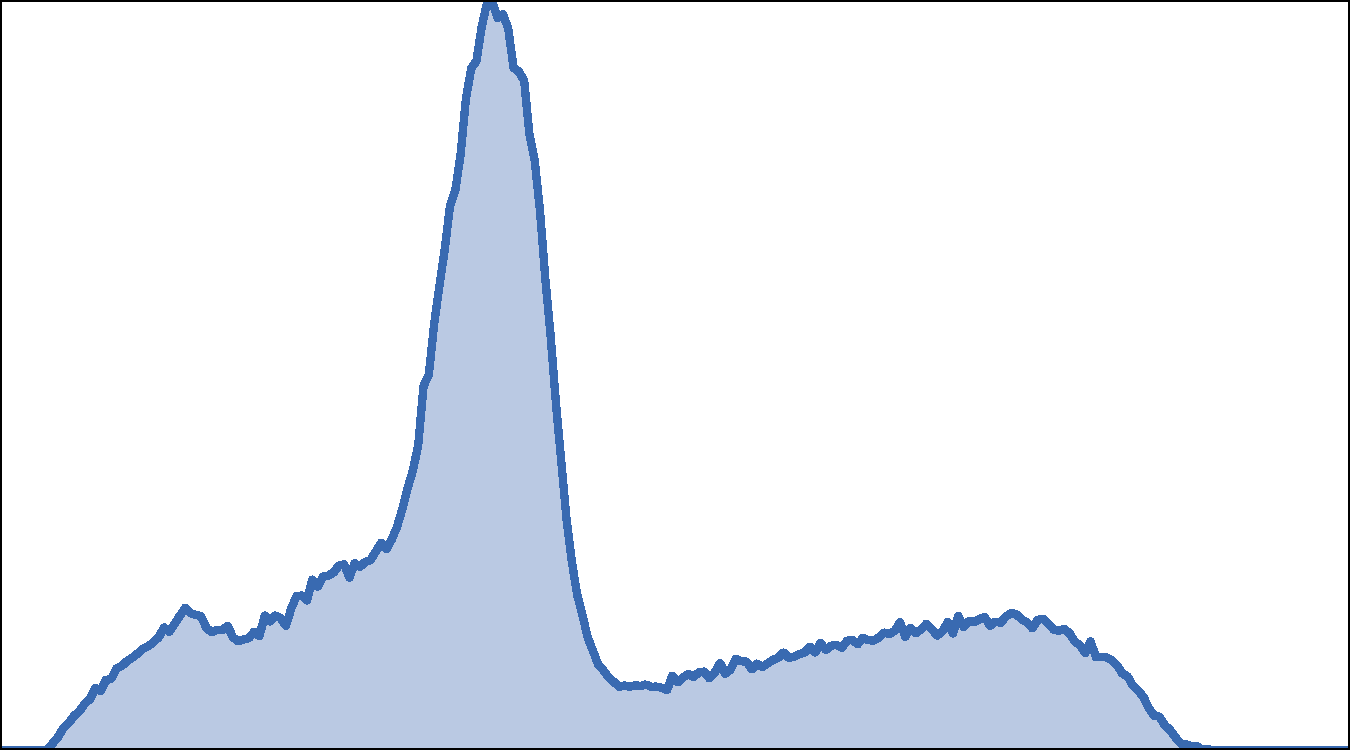
\includegraphics[width=0.3215\textwidth]{figures/hyd1_n00_hist.pdf}}
    \mbox{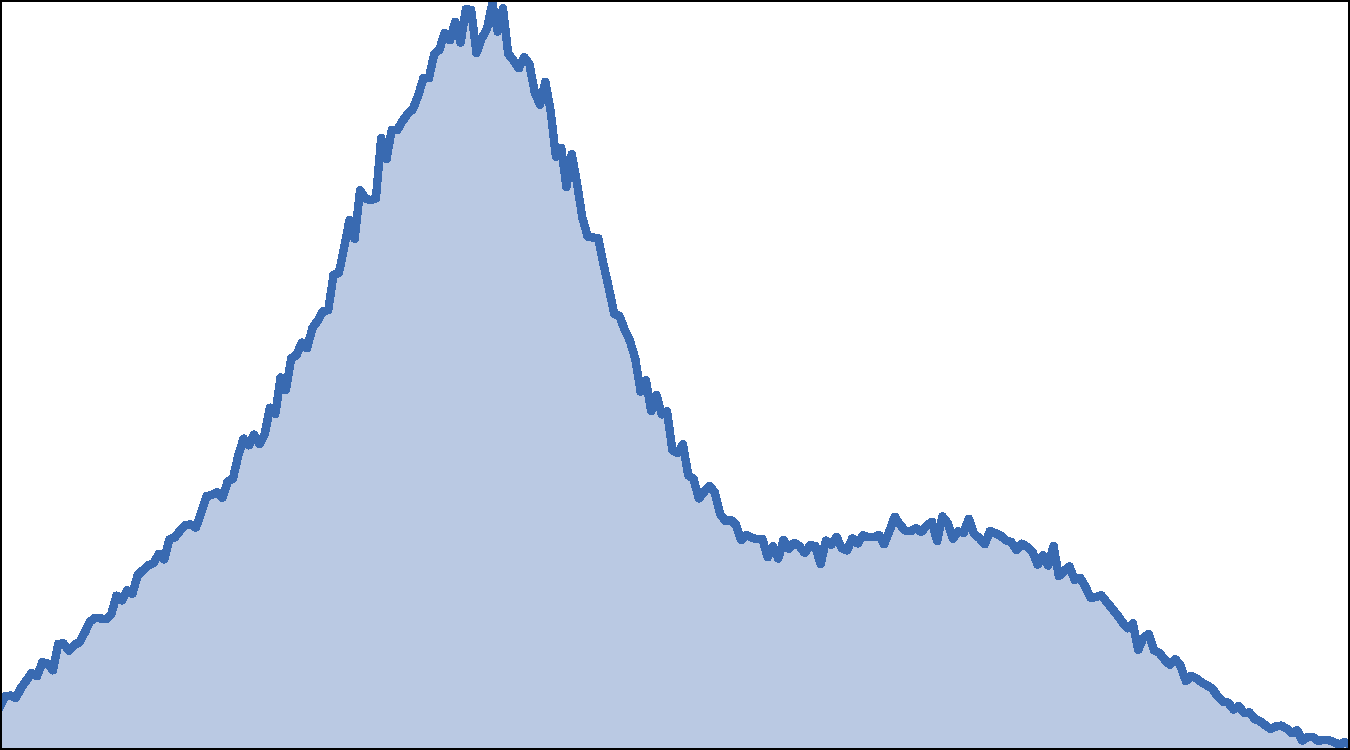
\includegraphics[width=0.3215\textwidth]{figures/hyd1_n20_hist.pdf}}
    \mbox{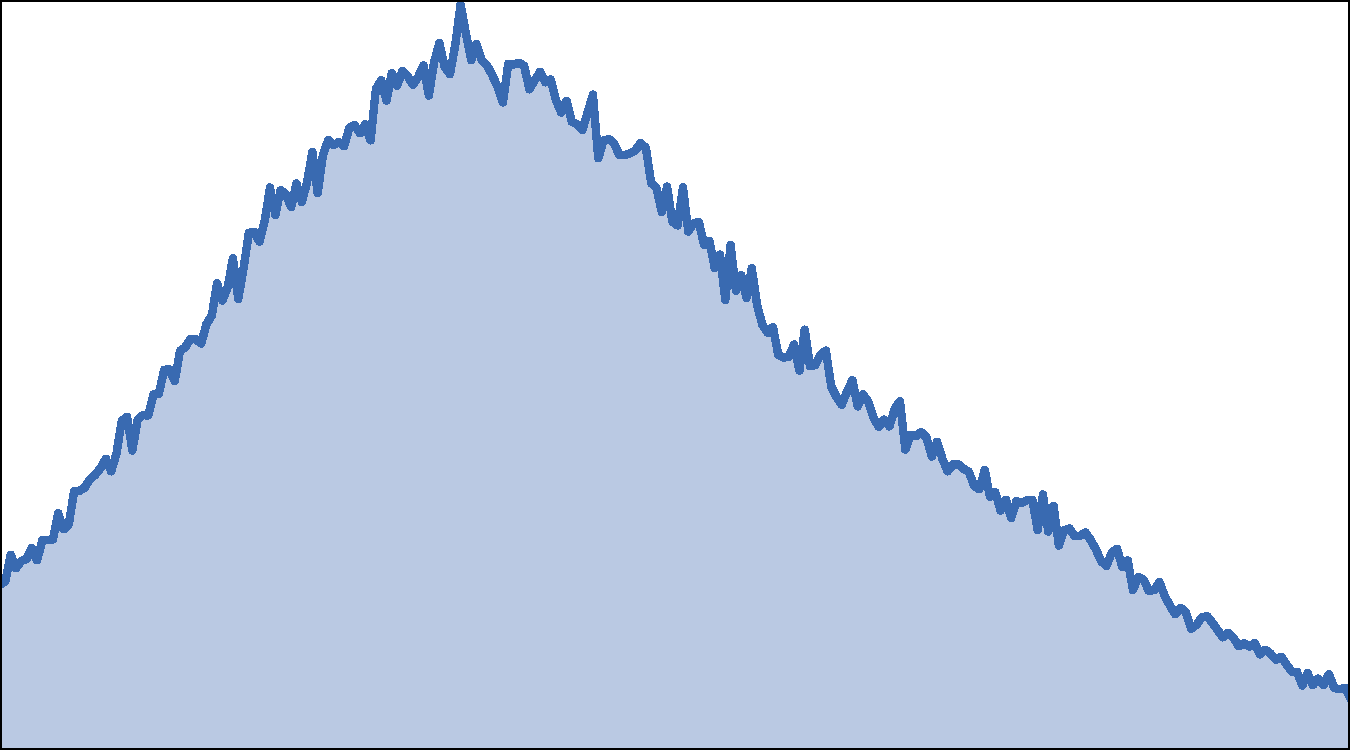
\includegraphics[width=0.3215\textwidth]{figures/hyd1_n40_hist.pdf}}
  }
  
  \centerline{
     	\mbox{
\includegraphics[scale=0.565]{figures/hist.png}}
     	\mbox{\includegraphics[scale=0.565]{figures/hist.png}}
     	\mbox{\includegraphics[scale=0.565]{figures/hist.png}}
  }
  \caption[Modeling noisy datasets]{Modeling noise for the \hyd dataset using the \textit{Gaussian} noise model. \textbf{(a)} First frame of the original image sequence. \textbf{(b)} Image with added Gaussian noise with standard deviation $\sigma = 20$. \textbf{(c)} Image with added Gaussian noise with standard deviation $\sigma = 40$. \textbf{Bottom Row:} Corresponding histograms. Note a dramatic change in the grey value distribution as a result of noise.}
  \label{fig:noisy}
\end{figure*}




\begin{figure*}[h]
%  \centerline{
%    \mbox{\includegraphics[scale=1.0]{figures/plot_noise_level_evaluation.png}}
%  }
    \centering
    \includegraphics[width=\textwidth]{figures/exp_noise_comp_3_datasets.pdf}
  
  \caption[Noise evaluation]{Evaluation of optical flow performance on noisy data with \textit{Gaussian} noise. For all datasets an average endpoint error (AEE) is shown in 3 regions: \textit{All} region is depicted as a green plot; \textit{Untext} region as a blue plot and \textit{Disc} region as a red plot.  \textbf{Left:} \rub dataset. \textbf{Middle:} \hyd dataset. \textbf{Right:} \mar dataset. Method: \textit{Baseline} algorithm (See Section \ref{baseline_method}).}
  \label{fig:noise_evaluation}
\end{figure*}


Datasets with synthetically added noise will be used for the quantitative evaluation in the following sections :
\begin{itemize}
 \item In Section \ref{experiment_noise_reduction} to show how noise affects the performance of \opticalflow and to evaluate different noise reduction approaches presented in Section \ref{contrast_adjustment}.
 
 \item In Section \ref{experiment_data_terms_for_noisy_data} to make a comparison between simple and higher-order data constancy assumptions and draw the conclusions about which of them are more robust w.r.t. to noisy data.
 
 \item In Section \ref{experimen_combined_local_global_approach} we evaluate the influence of incorporating the local information into the data term (CLG approach).
 
 \item In Section \ref{experiment_normalization_data_term} we study the result of data normalisation and its implication on the accuracy of flow computation.
 
\end{itemize}

 

\subsubsection{Contrast Level}
\label{model_contrast_level}

Another important property to evaluate is contrast. Since the X-ray data exhibits a wide range of image contrast levels (depending on imaging parameters), it is crucial to simulate and estimate the influence of image contrast on the performance of \opticalflow methods. 

To implement various contrast levels we take the original image sequence and reduce the contrast via the histogram rebinning while keeping the original values of maximum and minimum of the original histogram. An example of contrast reduction is illustrated in Figure \ref{fig:contrast_level}. 


%\change{Additionally, we estimate the performance of OF on such a image quality metric as Contrast-to-noise ratio and argue that such characteristics is very important while working with X-ray images.}

\begin{figure*}[!ht]
  \centerline{
    \mbox{\includegraphicslabeledw[scale=0.25]{figures/hyd1_c_000.png}{a}}
    \mbox{\includegraphicslabeledw[scale=0.25]{figures/hyd1_c_100.png}{b}}
    \mbox{\includegraphicslabeledw[scale=0.25]{figures/hyd1_c_200.png}{c}}
    }   
     \vspace{3pt}
   \centerline{
   	\mbox{\includegraphics[width=0.3215\textwidth]{figures/hyd1_n00_hist.pdf}}
   	\mbox{\includegraphics[width=0.3215\textwidth]{figures/hyd1_c_100_hist.pdf}}
   	\mbox{\includegraphics[width=0.3215\textwidth]{figures/hyd1_c_200_hist.pdf}}
   }
   
   \centerline{
   	\mbox{\includegraphics[scale=0.565]{figures/hist.png}}
   	\mbox{\includegraphics[scale=0.565]{figures/hist.png}}
   	\mbox{\includegraphics[scale=0.565]{figures/hist.png}}
   }
  \caption[Modeling contrast]{Modeling datasets with low feature contrast. \textbf{(a)} First frame of the original sequence. Contrast level $C = 100\%$. \textbf{(b)} Image with the reduced contrast.  Contrast level $C = 25\%$. \textbf{(c)} Contrast level $C = 12.5\%$. \textbf{Bottom Row:} Corresponding histograms showing a reduction in the dynamic range and, as a result, in the contrast level.}
  \label{fig:contrast_level}
\end{figure*}

To justify the importance of investigation of contrast changes on the results of motion estimation we perform an experiment in a similar fashion as we did with the previous experiment. We take a fixed optical flow model (\textit{baseline} method) and evaluate its performance on the images with different contrast values, varying it from $100\%$ of contrast to $7.5\%$. The evaluation plots are shown in Figure \ref{fig:noise_evaluation}.
Analysing them we can make the following conclusions:
\begin{itemize}
	\item The shrinkage of the dynamic range and a loss of useful information causes a severe degradation of the accuracy of optical flow results. For the substantial decrease in contrast the performance drop is significant and can be compared with the influence of noise. That is why even for low noise image data, an appropriate adjustment of computation parameters is required. 
	
	\item \hyd dataset contains a large amount of textural information in all image regions, as a result it is the easiest dataset to process, even in the case of low-contrast data.
	
\end{itemize}




\begin{figure*}[h]
%  \centerline{
%    \mbox{\includegraphics[scale=1.0]{figures/plot_noise_level_evaluation.png}}
%  }
    \centering
    \includegraphics[width=\textwidth]{figures/exp_contrast_comp_3_datasets.pdf}
  
  \caption[Fixed vs Optimal]{Evaluation of optical flow performance on 
 datasets with degraded  contrast level. For all datasets an average endpoint error (AEE) is shown in 3 regions: \textit{All} region is depicted as a green plot; \textit{Untext} region as a blue plot and \textit{Disc} region as a red plot.  \textbf{Left:} \rub dataset. \textbf{Middle:} \hyd dataset. \textbf{Right:} \mar dataset. Method: \textit{Baseline} algorithm.}
  \label{fig:contrast_evaluation}
\end{figure*}

We will use the datasets with the low-contrast in the following experiments:
\begin{itemize}

 \item In Section \ref{experiment_local_contrast} to show how a decrease in the image contrast affects the performance of \opticalflow, as well as to evaluate different contrast enhancement  approaches presented in Section \ref{contrast_adjustment}.
 
  \item In Section \ref{experiment_data_terms_for_contrast_data} to check the performance of different data terms, make comparison between them and draw conclusions about the data terms which are more robust with respect to low-contrast data.

  \item In Section \ref{experiment_robust_data_term_low_contrast} to evaluate the influence of robustification of the data term for low contrast image data.
 
\end{itemize}



\subsubsection{Brightness Changes}
\label{modeling_brigntenss}

In this section we describe different types of illumination changes, which may occur in X-ray data. Since the assumptions about brightness distribution of the scene and objects is the core information for the construction of data terms, any changes in brightness or illumination are important to take into account for the design of optical flow model or data preprocessing.

In this work we consider the following models of illumination changes:
\begin{itemize}
  \item Global additive illumination. For this case a constant value of $A$ is added to every pixel of the second image of the input sequence.
  \item Global multiplicative illumination. Every pixel of the second image frame is multiplied by a factor $M$. It is important to note, that changes in exposure time are corresponding to global multiplicative brightness change, thus is very important to model.
  \item Smooth spatial variation. We consider two patterns:  \textit{"Spot"}, resembling changing beam spot and \textit{"Strips"} pattern, simulating horizontal brightness flickering due to instability of a monochromator.
\end{itemize}

Two spatial patterns intended to simulate the uneven brightness distribution are presented in Figure \ref{fig:patterns}.

\newcommand{\patternsSize}{0.25}

\begin{figure*}[!ht]
  \centerline{
    \mbox{\includegraphicslabeledw[scale=\patternsSize]{figures/rub1.png}{a}}
    \mbox{\includegraphicslabeledw[scale=\patternsSize]{figures/rub2.png}{b}}
    \mbox{\includegraphicslabeledw[scale=\patternsSize]{figures/diff_original.png}{c}}
  }
  \vspace{3pt}
  \centerline{
    \mbox{\includegraphicslabeledb[scale=\patternsSize]{figures/pattern_circle_transparent.png}{d}}
    \mbox{\includegraphicslabeledw[scale=\patternsSize]{figures/pattern_circle_2.png}{e}}
    \mbox{\includegraphicslabeledw[scale=\patternsSize]{figures/diff_pattern_circle.png}{f}}
  }
  \vspace{3pt}
  \centerline{
    \mbox{\includegraphicslabeledw[scale=\patternsSize]{figures/pattern_strip_1.png}{g}}
    \mbox{\includegraphicslabeledw[scale=\patternsSize]{figures/pattern_strip_2.png}{h}}
    \mbox{\includegraphicslabeledw[scale=\patternsSize]{figures/diff_pattern_strip.png}{i}}
  }
  \caption[Modeling contrast]{Modeling illumination changes. \textbf{(a)} First frame of the original sequence. \textbf{(b)}  Second frame. \textbf{(c)}  Difference between original images that shows amount of brightness changes in a scene due to the actual movement. \textbf{(d)} The brightness pattern  added to the first frame. In this case its is transparent, so there is no modification of pixel values. \textbf{(e)} A \textit{"Spot"} brightness pattern added to the second frame. \textbf{(f)} Image changes due to the \textit{"Spot"} brightness pattern. \textbf{(g)}  The first part of the \textit{"Strips"} brightness pattern, added to the first frame. \textbf{(h)} The second part of the \textit{"Strips"} brightness pattern. \textbf{(i)} Changes due to the \textit{"Strips"} brightness pattern.}
  \label{fig:patterns}
\end{figure*}


We use datasets with the simulated brightness changes for the following evaluation experiments:

\begin{itemize}
	
	\item In Section \ref{experiment_nonuniform_brightness} to show the performance and usefulness of the brightness corrections techniques.
	
	\item In Section \ref{exp_data_terms_brighntness} to check the performance of different data terms for various brightness changes scenarios. 
	
	\item In Section \ref{experiment_robust_data_term_low_contrast} to evaluate the influence of robustification of the data term for low contrast image data.
	
\end{itemize}


\subsubsection{Image Artifacts}

The last step to complete our framework for quantitative evaluation is to provide the simulation of image artifacts. As it was mentioned previously, there are two prevalent artifacts in the X-ray data, which corrupt image data - ring artifacts and star (or streaks) artifacts. The main requirement for the modelling of such artifacts is that their location and the degree to which these artifacts affect the original data must be controlled.    
In this work we employ a simple model using geometric shapes similar to original effects. We control the placement of such artifacts and gradually increase the thickness of shapes to influence the intensity of the artifacts.

In this work we use the following artifacts structures:
\begin{itemize}
	\item Line shapes. These artifacts intended to mimic star artifacts (See Section \ref{image_artifacts}).  
	\item Circular shapes. These artifacts intended to model ring artifacts (See Section \ref{image_artifacts}).
	\item Dead pixels, dust and scratches artifacts. These artifacts are modelled using \textit{Spike} noise and were presented in Section \ref{modeling_image_noise}.
\end{itemize}

Images with the artificially modelled artifacts intended to simulate image degradation by means of ring or star artifacts are presented in Figure \ref{fig:artifacts}.

We use datasets with the simulated artifacts to perform quantitative evaluation in the following experiments:

\begin{itemize}
	
	\item In Section \ref{experiment_robust_data_term_artifacts}  to check the performance of the robust data term in the presence of image artifacts.
	
	\item In Section \ref{exp_flow_median} to evaluate the approach of median filtering and its influence on the accuracy of the optical flow.
	
	\item In Section \ref{exp_data_refinement} to evaluate the performance of the data refinement procedure.
	
\end{itemize}

	
\newcommand{\patternsSizew}{0.25}

\begin{figure*}[!ht]
	\centerline{
		\mbox{\includegraphicslabeledw[scale=\patternsSizew]{figures/rub1.png}{a}}
		\mbox{\includegraphicslabeledw[scale=\patternsSizew]{figures/rub2.png}{b}}
		\mbox{\includegraphicslabeledw[scale=\patternsSizew]{figures/diff_original.png}{c}}
	}
	\vspace{3pt}
	\centerline{
		\mbox{\includegraphicslabeledw[scale=\patternsSizew]{figures/rub1_a_1.png}{d}}
		\mbox{\includegraphicslabeledw[scale=\patternsSizew]{figures/rub2_a_1.png}{e}}
		\mbox{\includegraphicslabeledw[scale=\patternsSizew]{figures/artifacts_a1_diff.png}{f}}
	}
	\vspace{3pt}
	\centerline{
		\mbox{\includegraphicslabeledw[scale=\patternsSizew]{figures/rub1_a_4.png}{g}}
		\mbox{\includegraphicslabeledw[scale=\patternsSizew]{figures/rub1_a_4.png}{h}}
		\mbox{\includegraphicslabeledw[scale=\patternsSizew]{figures/artifacts_a4_diff.png}{i}}
	}
	\caption[Modeling contrast]{Modeling image artifacts. \textbf{(a)} First frame of original sequence. \textbf{(b)}  Second frame of original sequence. \textbf{(c)}  Difference between original images that shows amount of brightness changes in the original scene due to actual movement. \textbf{(d)} First image frame with artifacts. The thickness of artifacts is  $A=1$ pixel.  \textbf{(e)} Second image frame with artifacts $A=1$.  \textbf{(f)} Corresponding image difference which reveals the affected areas. \textbf{(g)} First image frame with artifacts. The thickness of artifacts is  $A=4$ pixels.  \textbf{(h)} Second image frame with artifacts $A=4$.  \textbf{(i)} Corresponding image difference. }
	\label{fig:artifacts}
\end{figure*}


%--------------------------------------------------------
\section{Optimization of Parameters}
\label{parameters_optimization}
%--------------------------------------------------------

In the section dedicated to data taxonomy we described a variety of X-ray data. In the previous section we showed how the performance of optical flow methods can be governed by the choice of model parameters (on the example of noisy images \ref{modeling_image_noise}  and low-contrast data \ref{model_contrast_level}). Therefore, parameters optimization become a critical and challenging task. For example, from the literature on optical flow methods it is well-known that appropriate choice of the smoothness parameter is important to obtain desirable results. However, there is remarkably little work on methods which allow to select or estimate optimal parameters. Only recently in the work of \cite{HarmonyFlow} the authors presented an approach for automatic smoothness parameters estimation based on the optimal prediction principle (See Section \ref{optimal_prediction_principle}). In our work we evaluate more approaches and confidence metrics (See Section \ref{confidence_measures}).
In this section we discuss numerous aspects of parameter optimization. 

%\begin{figure*}[h]
%  \centerline{
%    \mbox{\includegraphics[scale=0.6]{figures/exp_noise_rub.png}}
%  }
%  \caption[Fixed vs Optimal]{\todo{Update image and caption} Comparison between optimized and fixed parameters models on noisy \textit{Dataset 1}  \textbf{Top Left:} First frame of original sequence. \textbf{Top Right:}  Parameter +1. \textbf{Bottom Left:} Parameter +2. \textbf{Bottom Right:} Parameter +3.}
%  \label{fig:noise_fixed_optimal}
%\end{figure*}

%\comment{1. Take baseline algorithm with the best parameters (without optimisations) to show performance drop.
%\textbf{Run:} For each dataset: For all input images (noise): run on fixed parameter set } 
%
%\comment{2. Take baseline algorithm. Parameters: robust, flow-driven, no CLG, no median. Optimize alpha, sigma for each run
%\textbf{Run:} For each dataset: For all input images (noise): run with parameter optimization }


%\change{Another important aspect when showing the results of optical flow computation with or without a ground truth is to present not only the full description of the model used for the computation, but also a  model parameters. However, this is also not enough. If the parameters were optimisazed, a full range of parameters and optimization strategy should also be given.  
%Such situation does not happening in the literature during evaluation of the algorithms, which clearly limits the transparency a of the experimental conditions.}

%\subsection{Optimization of a Single Parameter}
\subsection{Optimization of Individual Parameter}

First we start with the evaluate and discussion of different model parameters of optical flow computation. The aim is to identify the set of paramters which are general and allow to obtain accurate and robust results. Selecting the best paramters we obtain a basis for our \textit{baseline method} which will be presented later in the chapter (See Section \ref{baseline_method}). Moreover, during the evaluation we highlight the importance of such optimization and provide a general guidance to perform it. Here we evaluate the most basis components of optical flow computation, such as derivatives approximation, number of warping levels and warping scale factor.




\subsubsection{Derivatives Approximation}

In Section \ref{discretization} a number of alternatives to represent image derivatives were outlined. Here we  compare different stencil modes and draw the conclusions about their appropriate usage for different image properties. For that, we consider two important aspects from our Data Taxonomy Section \ref{data_taxonomy}, namely the influence of noise and low contrast (low spatial image gradient). To check the performance on noisy data we restrict our study to \textit{Gaussian noise} model \ref{noise_models}, since it introduces sufficient disturbances to the image data.
For the evaluation we fix all the model parameters (which were optimized ahead), and vary only the computation schemes for derivatives approximation. The results for noisy data are shown in Table \ref{tab:derivatives_noise} and for low-contrast data in Table \ref{tab:derivatives_contrast}. 

With respect to noisy data we can make the following observations: 
\begin{itemize}
	\item \textit{Temporal averaging improves the results}. From the evaluation result we conclude that temporal averaging of is useful for both original and noise datasets and provided a robust scheme for derivatives. However, one should be confident that the displacements between corresponding image pairs are small, so such step could be performed. In the presence of large displacements we employ multi-level strategy, discussed in Section \ref{multilevel}. The appropriate choice for the warping scale and number of warping levels we discuss in Section \ref{opt_warping_scale} and Section \ref{opt_warping_levels} respectively. 
	\item \textit{Increased sensitivity of fourth-order derivatives to noise}. Despite the facts, that fourth-order derivatives approximation may lead to a significant improvements in accuracy for the original, noise-free images, it does not perform well on noise data. In the presence of noise a second-order approximation performs better for all noise levels. This might be explained by the increased sensitivity of the fourth order-derivative scheme to noise.
\end{itemize}
    
      
% Table generated by Excel2LaTeX from sheet 'noise'
\begin{table}[ht] \scriptsize
  \centering
  \caption{Comparison between spatial derivatives approximation schemes on noisy \rub dataset. The following computation schemes are compared:  second-order, second-order with temporal averaging, fourth order and fourth-order with temporal averaging. An additive \textit{Gaussian noise} with a zero-mean and standard deviations $\sigma$=0, 5, 10, 20 was introduced.}
    \begin{tabular}{ccccc}
    \toprule
    %\hline
    \multicolumn{1}{c}{noise} & \multicolumn{1}{ c}{model} & \multicolumn{3}{c}{error} \\ 
    \midrule
          &       & \textit{all}    & \textit{disc}   & \textit{untext}  \\ 
    \midrule
     \midrule
    \multicolumn{1}{c}{\multirow{4}[0]{*}{$\sigma$ = 0}} & \multicolumn{1}{l}{2nd order} & 0.172 & 0.683 & 0.135 \\
    \multicolumn{1}{c}{} & \multicolumn{1}{l}{2nd order + temp} & 0.161 & 0.628 & 0.13 \\
    \multicolumn{1}{c}{} & \multicolumn{1}{l}{4th order} & 0.169 & 0.673 & 0.132 \\
    \multicolumn{1}{c}{} & \multicolumn{1}{l}{4th order + temp} & \textbf{0.157} & \textbf{0.605} & \textbf{0.127} \\ 
    \midrule
    \multicolumn{1}{c}{\multirow{4}[0]{*}{$\sigma$ = 5}} & \multicolumn{1}{l}{2nd order} & 0.315 & 0.822 & 0.289 \\
    \multicolumn{1}{c}{} & \multicolumn{1}{l}{2nd order + temp} & \textbf{0.284} & \textbf{0.748} & \textbf{0.264} \\
    \multicolumn{1}{c}{} & \multicolumn{1}{l}{4th order} & 0.343 & 0.841 & 0.311 \\
    \multicolumn{1}{c}{} & \multicolumn{1}{l}{4th order + temp} & 0.304 & 0.751 & 0.273 \\
    \midrule
    \multicolumn{1}{c}{\multirow{4}[0]{*}{$\sigma$ = 10}} & \multicolumn{1}{l}{2nd order} & 0.581 & 1     & 0.544 \\
    \multicolumn{1}{c}{} & \multicolumn{1}{l}{2nd order + temp} & \textbf{0.506} & \textbf{0.921} & \textbf{0.454} \\
    \multicolumn{1}{c}{} & \multicolumn{1}{l}{4th order} & 0.664 & 1.037 & 0.652 \\
    \multicolumn{1}{c}{} & \multicolumn{1}{l}{4th order + temp} & 0.593 & 0.951 & 0.564 \\
    \midrule
    \multicolumn{1}{c}{\multirow{4}[1]{*}{$\sigma$ = 20}} & \multicolumn{1}{l}{2nd order} & 1.414 & 1.584 & 1.508 \\
    \multicolumn{1}{c}{} & \multicolumn{1}{l}{2nd order + temp} & \textbf{1.317} & \textbf{1.502} & \textbf{1.416} \\
    \multicolumn{1}{c}{} & \multicolumn{1}{l}{4th order} & 1.494 & 1.622 & 1.63 \\
    \multicolumn{1}{c}{} & \multicolumn{1}{l}{4th order + temp} & 1.45  & 1.576 & 1.6 \\
    \bottomrule
    \end{tabular}%
  \label{tab:derivatives_noise}%
\end{table}%

We can make the following conclusions about influence of different derivatives approximations on data with low contrast:
\begin{itemize}
	\item \textit{Usefulness of temporal averaging}. The same as for the case of noisy data, temporal averaging show to be effective to improve the accuracy of the optical flow computation. 
	\item \textit{Improved accuracy using fourth-order derivatives}. The accuracy of optical flow computation is improved using fourth-order derivatives approximation.
\end{itemize}

The evaluation of derivatives approximation schemes on \hyd and \mar datasets shows similar outcomes.  
Summarizing both experimental results we may conclude the following: in the presence of substantial noise we choose second-order derivatives with temporal averaging, if noise level is low or can be significantly reduced using preprocessing step we opt to use fourth-order derivatives with temporal averaging. 




% Table generated by Excel2LaTeX from sheet 'contrast'
\begin{table}[ht] \scriptsize
  \centering
  \caption{Comparison between spatial derivatives approximation schemes on  \rub dataset with low contrast. The following computation schemes are compared:  second-order, second-order with temporal averaging, fourth order and fourth-order with temporal averaging. A decrease to a contrast level of $C$=100\%, 50\%, 25\%, 10\% was introduced.}
    \begin{tabular}{ccccc}
    \toprule
    \multicolumn{1}{c}{contrast} & \multicolumn{1}{c}{model} & \multicolumn{3}{c}{error} \\
    \midrule
          &       & \multicolumn{1}{c}{\textit{all}} & \multicolumn{1}{c}{\textit{disc}} & \multicolumn{1}{c}{\textit{untext}} \\
          \midrule
          \midrule
    \multicolumn{1}{c}{\multirow{4}[0]{*}{$C$ = 100\%}} & \multicolumn{1}{l}{2nd order} & 0.172 & 0.683 & 0.135 \\
    \multicolumn{1}{c}{} & \multicolumn{1}{l}{2nd order + temp} & 0.161 & 0.628 & 0.13 \\
    \multicolumn{1}{c}{} & \multicolumn{1}{l}{4th order} & 0.169 & 0.673 & 0.132 \\
    \multicolumn{1}{c}{} & \multicolumn{1}{l}{4th order + temp} & \textbf{0.157} & \textbf{0.605} & \textbf{0.127} \\
     \midrule
    \multicolumn{1}{c}{\multirow{4}[0]{*}{$C$ = 50\%}} & \multicolumn{1}{l}{2nd order} & 0.224 & 0.681 & 0.238 \\
    \multicolumn{1}{c}{} & \multicolumn{1}{l}{2nd order + temp} & 0.214 & 0.667 & 0.223 \\
    \multicolumn{1}{c}{} & \multicolumn{1}{l}{4th order} & 0.207 & 0.662 & 0.213 \\
    \multicolumn{1}{c}{} & \multicolumn{1}{l}{4th order + temp} & \textbf{0.193} & \textbf{0.64} & \textbf{0.195} \\
     \midrule
    \multicolumn{1}{c}{\multirow{4}[0]{*}{$C$ = 25\%}} & \multicolumn{1}{l}{2nd order} & 0.3   & 0.729 & 0.348 \\
    \multicolumn{1}{c}{} & \multicolumn{1}{l}{2nd order + temp} & 0.293 & 0.721 & 0.334 \\
    \multicolumn{1}{c}{} & \multicolumn{1}{l}{4th order} & 0.284 & 0.717 & 0.325 \\
    \multicolumn{1}{c}{} & \multicolumn{1}{l}{4th order + temp} & \textbf{0.275} & \textbf{0.707} & \textbf{0.308} \\
     \midrule
    \multicolumn{1}{c}{\multirow{4}[0]{*}{$C$ = 10\%}} & \multicolumn{1}{l}{2nd order} & 0.41  & 0.797 & 0.48 \\
    \multicolumn{1}{c}{} & \multicolumn{1}{l}{2nd order + temp} & 0.398 & 0.791 & 0.461 \\
    \multicolumn{1}{c}{} & \multicolumn{1}{l}{4th order} & 0.385 & 0.785 & 0.451 \\
    \multicolumn{1}{c}{} & \multicolumn{1}{l}{4th order + temp} & \textbf{0.372} & \textbf{0.776} & \textbf{0.427} \\
    \bottomrule
    \end{tabular}%
  \label{tab:derivatives_contrast}%
\end{table}%




\subsubsection{Warping Levels}
\label{opt_warping_levels}

In order to deal with large displacements  according to our multi-level computation strategy (Section \ref{multilevel}) one has to construct image pyramid. For that purpose a scaling function is used which transfers the original image version to a coarser resolution level and interpolates the obtained results back to the finer computation level. Thus, on each computation level $k$ the image size is determined via:
$$ N^k_{d} = N^{orig} _{d} \eta^k,$$
where $\eta$ is a warping scale parameter, $N_d$ denotes the image size in the dimension $d \in (x,y)$.
In general, to get the best results and capture whole range of displacements (including the fastest motion) one may downscale the image as much as possible. However, for large images with small or moderate displacement values this strategy could result in a substantial loss of performance in terms of computation time. In fact, the aim is to downscale the original image in such a way, that the large displacements become small-scale on the lowest resolution level, so the linearized data constancy assumption can be employed. As soon as it is achieved, further downscaling provide no additional improvement. We illustrate this situation on the \rub dataset in Figure \ref{fig:opt_warping_levels}. Ideally, if the motion model is know or can be deduced from the original image sequence, it is possible to extract the optimal coarsest image size (e.g. number of warping levels) automatically.

\begin{figure*}[ht]
  \centerline{
    \mbox{\includegraphics[width=0.45\textwidth]{figures/opt_warping_levels.pdf}}
    \mbox{\includegraphics[width=0.45\textwidth]{figures/exp_optimize_scaling_factor.pdf}}
  }  
  \caption{Dependence of optical flow accuracy on a number of levels (coarse scale size) and a scaling factor $\eta$. \textbf{Left:} Improvement of average endpoint error for decreased image size on the coarsest resolution level. All the parameters were fixed as for \textit{baseline} method, warping scale factor $\eta$ = 0.95. Note, that these is no further improvement after a certain scale factor is reached. \textbf{Right:} Improvement of average endpoint error for increasing scaling factor. All the parameters were fixed as for \textit{baseline} method, a number of required warping levels is chosen according to a minimum possible coarsest image size.}
  \label{fig:opt_warping_levels}
\end{figure*}

Here we propose to use two strategies:

\begin{itemize}
	\item \textit{Estimation based on maximum velocity}. We compute the coarsest resolution image size via $ N^k = N^{orig}*S_{max}$, where $S_{max}=\frac{1}{max(\textbf{w})}$ is a scale factor and $max(\textbf{w})$ represents maximum displacement value for the current image pair.
	\item \textit{Estimation based on mean velocity}. We compute in a similar manner as a previous measure, but using mean velocity. Such measure can be reasonable in case if it is known that objects are moving with similar velocities. To account for velocity variations we include the standard deviation value of the velocities distribution. The final measure reads  $ N^k = N^{orig}*S_{mean}$, where $S_{mean}=\frac{1}{mean(\textbf{w}) + std(\textbf{w})}$. 
\end{itemize}

We compare both measures in the Table \ref{tab:opt_derivatives}. How we compute $S_{best}$: we increase the amount of warping levels (decreased image size on the coarsest resolution level) as long as there is a substantial improvement (more then 0.001 for AEE measure and 0.1\% for RX1.0 measure).  

\begin{table}[ht] \scriptsize
\centering
\caption{Comparison of methods to select an appropriate number of warping levels for \textit{RubberWhale}, \hyd and \mar datasets.}
\begin{tabular}{ccccccc}
\toprule
dataset & max   & mean & std & $S_{best}$ & $S_{max}$ & $S_{mean}$   \\ 
\midrule
\midrule
\rub     & 4.616 & 1.236 & 0.505 & 0.7 & 0.22 & \textbf{0.57}  \\ 
\hyd     & 11.12 & 3.48 & 1.452  & 0.57 & 0.09 & \textbf{0.2}  \\ 
\mar     & 2.09  & 1.64 & 0.166  & 0.66 & 0.48 & \textbf{0.55} \\ 
\bottomrule
\end{tabular}
\label{tab:opt_derivatives}%
\end{table}

Conclusions about automated selection of coarsest resolution image size:
\begin{itemize}
	\item \textit{Maximum-based measure provides good results}. This measure provides a reasonable precision and adapts to the image size and correctly handles largest displacements,  but computations on the coarsest levels introduced by the measure can be redundant. This can be seen from the comparison between $S_{best}$ and $S_{max}$ for the \hyd dataset. By default, if we are interested in computing an accurate optical flow we choose this measure.
	\item \textit{Mean-value improves the computation time}. This measure improves the computation time by adapting image to the mean velocity magnitudes and consequently considering less image levels. This measure is closer to the $S_{best}$ scale factor, however could provide poor results for large displacements.    
\end{itemize}
  
 

\subsubsection{Warping Scale}
\label{opt_warping_scale}


In general, the warping scaling factor should be as small as possible to guarantee a smooth transfer between warping levels. However, to small value will result in a very large number of warping levels, hence find compromise. An influence of scaling factors on \rub dataset on the overall precision of optical flow is shown in Figure \ref{fig:opt_warping_levels}.

A range of values between 0.9 and 0.95 is a good compromise between accuracy and running time.

%------------------------
% Does not look useful
%------------------------

%
%\subsubsection{Number of Iterations [SKIP?]}
%
%Three strategies to choose an appropriate number of iteration for the optimization procedure: \ref{iterative_methods}:
%\begin{itemize}
%	\item fixed
%	\item adaptive
%	\item stooping criteria
%\end{itemize}
%
%For Rub - the more the better (dense flow), For Mar - inproves on disc, but gets a bit worse in all regions. \todo{Try on a sequence with homogeneous (smooth) background. Situation could be different}


%---------------------------------------------
%---------------------------------------------
% Include section on multiple paramters
%---------------------------------------------
%---------------------------------------------

\subsection{Optimization of Multiple Parameters}

In this section we generalize the idea of parameters optimization and extend it for multiple parameters.
To highlight the importance of optimization of all model parameters we show several experiments related to three modes of smoothness, namely - data smoothness via presmoothing parameter $\sigma$ (See Section \ref{general_model}), flow smoothness $\alpha$ (See Section \ref{smoothness_assumptions}) and integration scale $\rho$.
First, we optimize one individual parameters, then a pair of smoothness paramters, and finally all the paramters related to smoothness. The quantitative results are presented in Table \ref{tab:exp_smooth3}.  

Analysing the results it is evident that all there smoothness parameters are crucial to provide  accurate and reliable optical flow and should be optimized simultaneously.


%\begin{figure*}[ht]
%  
%  \centerline{
%    \mbox{\includegraphics[scale=0.26]{figures/exp_smooth3_a_s.png}}
%    \mbox{\includegraphics[scale=0.26]{figures/exp_smooth3_a_r.png}}
%    \mbox{\includegraphics[scale=0.26]{figures/exp_smooth3_s_r.png}}
%  }
%  \vspace{3pt}
%  \centerline{
%    \mbox{\includegraphics[scale=0.28]{figures/exp_smooth3_flows.png}}
%  }
%  
%  \caption[]{\todo{Change caption} Comparison between three smoothness modes for optical flow computation. \textbf{Left Column:} Optimization of $\alpha$ and $\sigma$ parameters. \textbf{Left Column:} Optimization of $\alpha$ and $\rho$ parameters. \textbf{Left Column:} Optimization of $\sigma$ and $\rho$ parameters. \textbf{Top Row:} The best optical flow result using color coding. \textbf{Bottom Row:} Dependence of corresponding parameters.}
%  \label{fig:exp_smooth3}
%\end{figure*}






\begin{table}[ht] \scriptsize
  \centering
  \caption{Comparison between optimization of a single and simultaneous optimization of several model parameters. As an example we use there kinds of smoothness parameters: data smoothness via presmoothing parameter ($\sigma$), flow smoothness ($\alpha$) and integration scale ($\rho$).}
    \begin{tabular}{rrcrrrrr}
    \toprule
    number & \multicolumn{1}{c}{model} & \multicolumn{3}{c}{error} & \multicolumn{3}{c}{model parameters} \\
    \midrule
              &       & \textit{all} & \multicolumn{1}{c}{\textit{disc}} & \multicolumn{1}{c}{\textit{untext}} & \multicolumn{1}{c}{\textit{alpha}} & \multicolumn{1}{c}{\textit{sigma}} & \multicolumn{1}{c}{\textit{rho}} \\
          \midrule
          \midrule
          
    \multirow{3}[0]{*}{one } & \multicolumn{1}{l}{optimize $\alpha$} & 0.349 & \multicolumn{1}{c}{\textbf{0.773}} & \multicolumn{1}{c}{0.392} & \multicolumn{1}{l}{7.5} & \multicolumn{1}{l}{0.35} & \multicolumn{1}{l}{--} \\
          & \multicolumn{1}{l}{optimize $\sigma$} & 0.437 & \multicolumn{1}{c}{0.876} & \multicolumn{1}{c}{0.362} & \multicolumn{1}{l}{3.5} & \multicolumn{1}{l}{0.6} & \multicolumn{1}{l}{--} \\      
              & \multicolumn{1}{l}{optimize $\rho$} & \textbf{0.305} & \multicolumn{1}{c}{0.833} & \multicolumn{1}{c}{\textbf{0.314}} & \multicolumn{1}{l}{3.5} & \multicolumn{1}{l}{0.35} & \multicolumn{1}{l}{4.6} \\
          
          \midrule
    \multirow{3}[0]{*}{two} & \multicolumn{1}{l}{optimize $\alpha, \sigma$} & 0.342 & \multicolumn{1}{c}{0.773} & \multicolumn{1}{c}{0.351} & \multicolumn{1}{l}{7.0} & \multicolumn{1}{l}{0.5} & \multicolumn{1}{l}{--} \\
    
          & \multicolumn{1}{l}{optimize $\alpha, \rho$} & 0.298 & \multicolumn{1}{c}{\textbf{0.754}} & \multicolumn{1}{c}{0.313} & \multicolumn{1}{l}{5.0} & \multicolumn{1}{l}{0.35} & \multicolumn{1}{l}{2.7} \\
          & \multicolumn{1}{l}{optimize $\sigma, \rho$} & \textbf{0.305} & \multicolumn{1}{c}{0.832} & \multicolumn{1}{c}{\textbf{0.304}} & \multicolumn{1}{l}{3.5} & \multicolumn{1}{l}{0.4} & \multicolumn{1}{l}{4.6} \\
          
          \midrule
          
    three   & \multicolumn{1}{l}{optimize $\alpha, \sigma, \rho$} & \textbf{0.297} & \multicolumn{1}{c}{\textbf{0.757}} & \multicolumn{1}{c}{\textbf{0.299}} & \multicolumn{1}{l}{4.75} & \multicolumn{1}{l}{0.4} & \multicolumn{1}{l}{3.1} \\
    \bottomrule
    \end{tabular}%
  \label{tab:exp_smooth3}%
\end{table}%




\subsection{Confidence-based Optimization}



In the previous two section we have based our parameters optimization procedure on the use of ground truth data, so we were able to compare the computed results with the real ones. For the real life data (tasks) such information is not available. For this purpose a measure based on the confidence can be used. In Section \ref{confidence_measures} a number of possible confidence measures were presented.

Here we demonstrate an example of comparison of metrics to evaluate the correctness of the result using average endpoint error \ref{endpoint_error} and data constancy error \ref{data_constancy_error}. We vary the paramter of the flow regularization $\alpha$ and measure both metrics. The results are presented in Figure \ref{fig:exp_confifance}.
As it can be observed, even without ground truth result it is possible to judge the reliability of the results and choose a sub-optimal parameter based on confidence-based optimization. 

% \begin{figure*}[ht]
% 	\centerline{
% 		\includegraphics[scale = 0.45]{figures/example_confidance_optimization.png} 
% 	}  
% 	\caption{Comparison between distribution of average endpoint error (AEE) for different values of smoothness parameter $\alpha$ using comparison with a ground truth (optimal) and error metric based on confidence measures.  \textbf{Left:} Average endpoint error given by the comparison of the computed flow field with the ground truth result (\textit{aee}). \textbf{Right:} Data Constancy Error measure (\textit{dev}).}
% 	\label{fig:example_confifance}
% \end{figure*} 

 We further evaluate these measures in the experimental section \ref{exp_confidence_evaluation} and draw conclusions about their appropriate usage. 



\subsection{Baseline Method}
\label{baseline_method}


As it was discussed in the introductory part of the current section, dedicated to parameter optimization, the performance of optical flow largely depends on the set of chosen of model parameters. Since advanced optical flow methods tend to incorporate many features into a single model, it is challenging to separate and evaluate the influence of the individual setting. To provide a basis for a systematic comparison of different settings and model parameters here we describe a \textit{baseline} method which we use in the following experiments section. In all parts where we refer to the baseline method we mean this set of settings.


\begin{table}[ht] \footnotesize
\centering
\caption{A list of all model parameters used for the \textit{baseline} method. If not presented explicitly, all the parameters of the \textit{baseline} method  correspond to the ones given in this table.}
\begin{tabular}{lp{3cm}cp{5cm}}
\toprule
Model parameter & Parameter name & Symbol & Value / Expression   \\ 
\midrule
\midrule
Constancy assumption    & grey value & $D_{grey}(I,\textbf{w})$ & $(\nabla_{3}^{\top}I\textbf{w})^2$ \\ 
Smoothness assumption   & flow-driven & $S_{flow}(u,v)$ & $\Psi_{S}(|\nabla u|^2 + |\nabla v|^2)$, $\Psi_{S}(x) = \sqrt{x + \epsilon}$, $\epsilon = 0.001$ \\ 
Robust function  & Charbonnier penalty & $D_{R}(I,\textbf{w})$ & $ \Psi_R ( (\nabla_{3}^{\top}I\textbf{w})^2)$, $\Psi_{R}(x) = \sqrt{x + \epsilon}$, $\epsilon = 0.001$ \\
Derivatives approximation & second-order and time averaging & $I_x, I_y$ & $\frac{(I_{i+1,j,t+1} - I_{i-1,j,t+1}) + (I_{i+1,j,t} - I_{i-1,j,t})  }{4 h_x}$ \\
Data normalization & -- & $ D_{norm}(I,\textbf{w})$ &  $ \frac{(\nabla_{3}^{\top}I\textbf{w})^2}{|\nabla_2 I(x,y,t)|^2 + \eta} $, disabled \\
Combined local-global & -- & $ D_{CLG}(I,\textbf{w})$ &  $K_{\rho} \ast (\nabla_{3}^{\top}I\textbf{w})^2$ , disabled \\
Median filtering & -- & $  M_p (\textbf{dw}^{k})$ &  $ p \in (3,5)$ , disabled \\
Flow regularization & smoothness parameter & $\alpha$ &  $3.5$ \\
Adaptive regularization & -- & $\alpha(k)$ &  $\alpha$, disabled \\
Presmoothing parameter & standard deviation & $\sigma$ &  $0.35$ \\
Multi-level scheme & warping levels & $k$ &  $15$ \\
Warping accuracy & warping scale & $\eta$ &  $0.9$ \\
\bottomrule
\end{tabular}
\label{tab:baseline}%
\end{table}





 
%--------------------------------------------------------
\section{Quantitative Evaluation}
\label{experiments_synthetic_data}
%--------------------------------------------------------

In this section we present a discussion on the performance, influence of preprocessing, modelling of noise and data outliers and the use of confidence measures. For each experimental evaluation we discuss the advantages and shortcomings of the proposed prototypes. All the results are presented in both a quantitative and a qualitative way. 
For all the experiments we outline important observations and draw the conclusions, which we summarize in the last section of the chapter (See Section \ref{experiments_summary}). In the summary table columns \textit{all}, \textit{disc} and \textit{untext} show the \textit{best possible} result for each region of statistics over the whole range of evaluated parameters.






%--------------------------------------------------------
\subsection{Experiments: Noise}
\label{exp_noise}
%--------------------------------------------------------

\subsubsection{Experiment: Data terms for noisy data}
\label{experiment_data_terms_for_noisy_data}


In this experiment we compare different data terms with respect to their performance on noisy data. To model noise we choose there models - Gaussian, Poisson and Spike noise (see Section \ref{noise_models}), which aim to represent different noise scenarios. While \textit{Gaussian noise} is commonly used in the literature on optical flow to test the robustness of methods in the presence of noise, it is still a simplified noise model. \textit{Poisson noise} is a physically based noise model and correctly describes X-ray data. Finally, \textit{Spike noise} represents a special type of noise with a severe level of image degradation and aims to model data artifacts. Details on the implementation of noise models are given in Section \ref{modeling_image_noise}. We evaluate the performance of data constancy assumptions on noisy data and present our results in Table \ref{tab:noise_data_terms}. For the evaluation we use the \textit{baseline} optical flow method with the optimized  smoothness parameter $\alpha$ and presmoothing parameter $\sigma$. 

% Table generated by Excel2LaTeX from sheet '__all__'
\begin{table}[htbp] \scriptsize
  \centering
  \caption{Performance analysis of data terms on noisy data on the \rub dataset. \textit{Gaussian noise} with zero mean and standard deviation values of $\sigma_n$ = 0, 5, 10, 20 was added. \textit{Poisson noise}: Mean value of the Poisson random distribution $P$ is 0, 50, 200, 400. \textit{Spike Noise}: we randomly replace a certain percentage of pixels with black and the same amount of pixels with white grey value. For the experiment an amount of $S=$0\% (no noise), 2.5\%, 5.0\%, 7.5\% replaced pixels was used. Method: \textit{baseline}, optimized for $\sigma=[0.15 .. 2.5]$, $\alpha=[1.0 .. 40]$.}
    \begin{tabular}{crrrrrrrrrrrr}
    \toprule
    model & \multicolumn{4}{c}{Gaussian noise} & \multicolumn{4}{c}{Poisson noise} & \multicolumn{4}{c}{Spike noise} \\
    \midrule
          & \multicolumn{1}{c}{$\sigma_n$} & \multicolumn{3}{c}{error} & \multicolumn{1}{c}{$P$} & \multicolumn{3}{c}{error} & \multicolumn{1}{c}{$S$} & \multicolumn{3}{c}{error} \\
          
          \midrule
          
          
          & \multicolumn{1}{c}{} & \multicolumn{1}{c}{\textit{all}} & \multicolumn{1}{c}{\textit{disc}} & \multicolumn{1}{c}{\textit{untext}} & \multicolumn{1}{c}{} & \multicolumn{1}{c}{\textit{all}} & \multicolumn{1}{c}{\textit{disc}} & \multicolumn{1}{c}{\textit{untext}} & \multicolumn{1}{c}{} & \multicolumn{1}{c}{\textit{all}} & \multicolumn{1}{c}{\textit{disc}} & \multicolumn{1}{c}{\textit{untext}} \\
          
          \midrule
          \midrule
          
    grey  & \multicolumn{1}{r}{\multirow{4}[1]{*}{0}} & \multicolumn{1}{c}{0.159} & \multicolumn{1}{c}{0.622} & \multicolumn{1}{c}{0.13} & \multicolumn{1}{r}{\multirow{4}[1]{*}{0}} & \multicolumn{1}{c}{0.159} & \multicolumn{1}{c}{0.622} & \multicolumn{1}{c}{0.13} & \multicolumn{1}{r}{\multirow{4}[1]{*}{0 \%}} & \multicolumn{1}{c}{0.159} & \multicolumn{1}{c}{0.622} & \multicolumn{1}{c}{0.13} \\
    grad  &       & \multicolumn{1}{c}{\textbf{0.11}} & \multicolumn{1}{c}{\textbf{0.526}} & \multicolumn{1}{c}{\textbf{0.073}} &       & \multicolumn{1}{c}{\textbf{0.11}} & \multicolumn{1}{c}{\textbf{0.526}} & \multicolumn{1}{c}{\textbf{0.073}} &       & \multicolumn{1}{c}{\textbf{0.11}} & \multicolumn{1}{c}{\textbf{0.526}} & \multicolumn{1}{c}{\textbf{0.073}} \\
    lapl  &       & \multicolumn{1}{c}{0.127} & \multicolumn{1}{c}{0.566} & \multicolumn{1}{c}{0.077} &       & \multicolumn{1}{c}{0.562} & \multicolumn{1}{c}{0.075} & \multicolumn{1}{c}{0.13} &       & \multicolumn{1}{c}{0.562} & \multicolumn{1}{c}{0.075} & \multicolumn{1}{c}{0.13} \\
    norm  &       & \multicolumn{1}{c}{0.137} & \multicolumn{1}{c}{0.607} & \multicolumn{1}{c}{0.095} &       & \multicolumn{1}{c}{0.602} & \multicolumn{1}{c}{0.094} & \multicolumn{1}{c}{0.201} &       & \multicolumn{1}{c}{0.602} & \multicolumn{1}{c}{0.094} & \multicolumn{1}{c}{0.201} \\
    
    \midrule
    
    grey  & \multicolumn{1}{r}{\multirow{4}[2]{*}{5}} & \multicolumn{1}{c}{0.26} & \multicolumn{1}{c}{0.722} & \multicolumn{1}{c}{0.261} & \multicolumn{1}{r}{\multirow{4}[2]{*}{50}} & \multicolumn{1}{c}{0.391} & \multicolumn{1}{c}{\textbf{0.798}} & \multicolumn{1}{c}{0.479} & \multicolumn{1}{r}{\multirow{4}[2]{*}{2.5\%}} & \multicolumn{1}{c}{\textbf{0.437}} & \multicolumn{1}{c}{0.838} & \multicolumn{1}{c}{0.576} \\
    grad  &       & \multicolumn{1}{c}{\textbf{0.233}} & \multicolumn{1}{c}{\textbf{0.689}} & \multicolumn{1}{c}{\textbf{0.242}} &       & \multicolumn{1}{c}{\textbf{0.383}} & \multicolumn{1}{c}{0.799} & \multicolumn{1}{c}{\textbf{0.416}} &       & \multicolumn{1}{c}{0.543} & \multicolumn{1}{c}{0.92} & \multicolumn{1}{c}{0.614} \\
    lapl  &       & \multicolumn{1}{c}{0.273} & \multicolumn{1}{c}{0.712} & \multicolumn{1}{c}{0.303} &       & \multicolumn{1}{c}{0.496} & \multicolumn{1}{c}{0.851} & \multicolumn{1}{c}{0.646} &       & \multicolumn{1}{c}{0.965} & \multicolumn{1}{c}{\textbf{0.74}} & \multicolumn{1}{c}{\textbf{0.099}} \\
    norm  &       & \multicolumn{1}{c}{0.269} & \multicolumn{1}{c}{0.729} & \multicolumn{1}{c}{0.272} &       & \multicolumn{1}{c}{0.395} & \multicolumn{1}{c}{0.809} & \multicolumn{1}{c}{0.464} &       & \multicolumn{1}{c}{0.937} & \multicolumn{1}{c}{0.658} & \multicolumn{1}{c}{0.104} \\
    
    \midrule
    
   
    grey  & \multicolumn{1}{r}{\multirow{4}[2]{*}{10}} & \multicolumn{1}{c}{0.346} & \multicolumn{1}{c}{0.774} & \multicolumn{1}{c}{0.359} & \multicolumn{1}{r}{\multirow{4}[2]{*}{200}} & \multicolumn{1}{c}{0.449} & \multicolumn{1}{c}{\textbf{0.848}} & \multicolumn{1}{c}{0.554} & \multicolumn{1}{r}{\multirow{4}[2]{*}{5.0\%}} & \multicolumn{1}{c}{\textbf{0.611}} & \multicolumn{1}{c}{0.902} & \multicolumn{1}{c}{0.683} \\
    grad  &       & \multicolumn{1}{c}{\textbf{0.331}} & \multicolumn{1}{c}{\textbf{0.767}} & \multicolumn{1}{c}{\textbf{0.346}} &       & \multicolumn{1}{c}{\textbf{0.44}} & \multicolumn{1}{c}{0.852} & \multicolumn{1}{c}{\textbf{0.497}} &       & \multicolumn{1}{c}{0.67} & \multicolumn{1}{c}{0.992} & \multicolumn{1}{c}{0.732} \\
    lapl  &       & \multicolumn{1}{c}{0.411} & \multicolumn{1}{c}{0.802} & \multicolumn{1}{c}{0.48} &       & \multicolumn{1}{c}{0.596} & \multicolumn{1}{c}{0.917} & \multicolumn{1}{c}{0.777} &       & \multicolumn{1}{c}{1.04} & \multicolumn{1}{c}{0.904} & \multicolumn{1}{c}{0.101} \\
    norm  &       & \multicolumn{1}{c}{0.351} & \multicolumn{1}{c}{0.791} & \multicolumn{1}{c}{0.377} &       & \multicolumn{1}{c}{0.467} & \multicolumn{1}{c}{0.873} & \multicolumn{1}{c}{0.556} &       & \multicolumn{1}{c}{1} & \multicolumn{1}{c}{\textbf{0.722}} & \multicolumn{1}{c}{\textbf{0.077}} \\
    
    \midrule
    
    grey  & \multicolumn{1}{r}{\multirow{4}[1]{*}{20}} & \multicolumn{1}{c}{0.474} & \multicolumn{1}{c}{0.866} & \multicolumn{1}{c}{0.567} & \multicolumn{1}{r}{\multirow{4}[1]{*}{400}} & \multicolumn{1}{c}{0.538} & \multicolumn{1}{c}{\textbf{0.897}} & \multicolumn{1}{c}{0.634} & \multicolumn{1}{r}{\multirow{4}[1]{*}{7.5\%}} & \multicolumn{1}{c}{\textbf{0.761}} & \multicolumn{1}{c}{0.978} & \multicolumn{1}{c}{0.733} \\
    grad  &       & \multicolumn{1}{c}{\textbf{0.462}} & \multicolumn{1}{c}{\textbf{0.866}} & \multicolumn{1}{c}{\textbf{0.545}} &       & \multicolumn{1}{c}{\textbf{0.53}} & \multicolumn{1}{c}{0.907} & \multicolumn{1}{c}{\textbf{0.589}} &       & \multicolumn{1}{c}{0.761} & \multicolumn{1}{c}{1.031} & \multicolumn{1}{c}{0.71} \\
    lapl  &       & \multicolumn{1}{c}{0.57} & \multicolumn{1}{c}{0.922} & \multicolumn{1}{c}{0.68} &       & \multicolumn{1}{c}{0.748} & \multicolumn{1}{c}{0.98} & \multicolumn{1}{c}{0.955} &       & \multicolumn{1}{c}{1.083} & \multicolumn{1}{c}{0.847} & \multicolumn{1}{c}{0.098} \\
    norm  &       & \multicolumn{1}{c}{0.471} & \multicolumn{1}{c}{0.882} & \multicolumn{1}{c}{0.566} &       & \multicolumn{1}{c}{0.545} & \multicolumn{1}{c}{0.918} & \multicolumn{1}{c}{0.618} &       & \multicolumn{1}{c}{1.044} & \multicolumn{1}{c}{\textbf{0.713}} & \multicolumn{1}{c}{\textbf{0.06}} \\
    \bottomrule
    \end{tabular}%
  \label{tab:noise_data_terms}%
\end{table}%


From the results of quantitative evaluation we can get the following conclusions:
\begin{itemize}
	\item \textit{Gradient constancy assumption with the robust setting provides good results for both Gaussian and Poisson noise models}. It is reasonable to assume that a derivatives-based constancy assumption will be more sensitive to noise, than a simple grey value assumption. In the work of \cite{BruhnThesis} it was shown that, indeed, the gradient based constancy assumption gives worse performance in comparison with the grey value assumption. However, in the evaluation perform in \cite{BruhnThesis} the robust data term was not used. From our performance analysis it is evident, that the gradient constancy assumption in a robust setting provides better results even for large amounts of noise in all image regions. 
	    
	\item \textit{Higher order derivatives are sensitive to noise for the Gaussian, Poisson and Spike noise models}. Both the Laplacian and Gradient norm constancy assumptions are very sensitive to noise and provide poor results. Thus, these data terms are not useful for X-ray data, which usually contains high amounts of noise. However, one should note, that for noise-free images these data terms outperform the grey value constancy assumption. 
	
	\item \textit{Grey value constancy assumption is more robust for the Spike noise model}. For the Spike noise model the situation is different from the Gaussian noise model. In this case, grey value constancy assumption is more robust to corrupted pixel data. One may notice, that in some cases high order constancy assumptions perform better in \textit{Disc} and \textit{Untext} image regions, however, this situation corresponds to the case when the largest values for smoothing parameters $\alpha$ and $\sigma$ are chosen. In this case the image was oversmoothed, which is seen from the values of \textit{AEE} measure in all image regions. 

	\item \textit{Grey value constancy assumption is more robust for the Spike noise model}. For this noise model the situation is different as for the Gaussian noise model. In this case, the grey value constancy assumption is more robust with respect to corrupted pixel data. One may notice, that in some cases high order constancy assumptions perform better in \textit{Disc} and \textit{Untext} image regions, however, this situation corresponds to the case when the largest values for smoothing parameters $\alpha$ and $\sigma$ are chosen. In this case the image was oversmoothed, which is seen from the values of \textit{AEE} measure in all image regions. 
	
	\item \textit{Grey value constancy assumption is more robust for the Poisson noise model in the regions of image discontinues}.  In general, the Poisson noise model is more challenging then the Gaussian noise model. This is due to the fact that the effect of Gaussian noise can be effectively removed with an appropriate image smoothing. Additionally, the evaluation of results shows that the grey value constancy assumption provides better performance in the regions of image discontinues.  
\end{itemize}





\subsubsection{Experiment: Combined local-global approach}
\label{experimen_combined_local_global_approach}


In this experiment we evaluate the performance of the Combined Local-Global (CLG) approach on noisy data. In the literature on optical flow methods such approaches are not commonly used, especially for synthetic datasets. However, as it was shown in the works of \cite{Bruhn02, Bruhn05a}, such approach can be beneficial in the presence of large amount of noise. We extend the evaluation presented in \cite{BruhnThesis} and perform quantitative evaluation for both the grey value and the gradient value constancy assumptions on \textit{Gaussian} and \textit{Spike} noise models. The evaluation results on the \rub dataset are presented in Table \ref{tab:exp_clg}. The evaluation results are similar for the \hyd and the \mar datasets and excluded from presentation. 





% Table generated by Excel2LaTeX from sheet 'res'
\begin{table}[ht] \scriptsize
  \centering
  \caption{Performance of the Combined Local-Global (CLG) approach on the \textit{Gaussian} and \textit{Spike} noise models on \rub dataset. \textit{Gaussian Noise} with zero mean  and standard deviation values of $\sigma_n$ = 5, 10, 20 was added. For \textit{Spike Noise} an amount $S$  of 2.5\%, 5.0\%, 7.5\% replaced pixels was used. Method: \textit{baseline}, optimized $\rho$ in the range $[0.5 .. 2.0]$, optimized $\sigma$ in the range $[0.35 .. 1.5]$, optimized $\alpha$ in the range $[3.0 .. 40]$.}
    \begin{tabular}{rrrrrrrrr}
    \toprule
          &       & \multicolumn{3}{c}{Gaussian noise} &       & \multicolumn{3}{c}{Spike noise} \\
    \midrule
    \multicolumn{1}{c}{model} & \multicolumn{1}{c}{$\sigma_n$} & \multicolumn{3}{c}{error} & \multicolumn{1}{c}{$S$} & \multicolumn{3}{c}{error} \\
    \midrule
    \multicolumn{1}{c}{} & \multicolumn{1}{c}{\textit{}} & \textit{all} & \multicolumn{1}{c}{\textit{disc}} & \multicolumn{1}{c}{\textit{untext}} & \multicolumn{1}{c}{\textit{}} & \textit{all} & \multicolumn{1}{c}{\textit{disc}} & \multicolumn{1}{c}{\textit{untext}} \\
    \midrule
    \midrule
    \multicolumn{1}{l}{grey} & \multicolumn{1}{c}{\multirow{4}[0]{*}{5}} & 0.26  & \multicolumn{1}{c}{0.722} & \multicolumn{1}{c}{0.261} & \multicolumn{1}{c}{\multirow{4}[0]{*}{2.5\%}} & 0.437 & \multicolumn{1}{c}{0.838} & \multicolumn{1}{c}{0.576} \\
    \multicolumn{1}{l}{grey+CLG} &       & \textbf{0.222} & \multicolumn{1}{c}{\textbf{0.706}} & \multicolumn{1}{c}{\textbf{0.219}} &       & \textbf{0.424} & \multicolumn{1}{c}{0.838} & \multicolumn{1}{c}{0.576} \\
    \multicolumn{1}{l}{grad} &       & 0.233 & \multicolumn{1}{c}{0.689} & \multicolumn{1}{c}{0.242} &       & 0.543 & \multicolumn{1}{c}{0.92} & \multicolumn{1}{c}{0.614} \\
    \multicolumn{1}{l}{grad+CLG} &       & \textbf{0.218} & \multicolumn{1}{c}{0.689} & \multicolumn{1}{c}{\textbf{0.235}} &       & \textbf{0.516} & \multicolumn{1}{c}{\textbf{0.916}} & \multicolumn{1}{c}{\textbf{0.588}} \\
    \midrule
    \multicolumn{1}{l}{grey} & \multicolumn{1}{c}{\multirow{4}[0]{*}{10}} & 0.346 & \multicolumn{1}{c}{0.774} & \multicolumn{1}{c}{0.359} & \multicolumn{1}{c}{\multirow{4}[0]{*}{5.0\%}} & 0.611 & \multicolumn{1}{c}{\textbf{0.902}} & \multicolumn{1}{c}{\textbf{0.683}} \\
    \multicolumn{1}{l}{grey+CLG} &       & \textbf{0.299} & \multicolumn{1}{c}{\textbf{0.755}} & \multicolumn{1}{c}{\textbf{0.3}} &       & \textbf{0.609} & \multicolumn{1}{c}{0.909} & \multicolumn{1}{c}{0.685} \\
    \multicolumn{1}{l}{grad} &       & 0.331 & \multicolumn{1}{c}{\textbf{0.767}} & \multicolumn{1}{c}{0.346} &       & 0.67  & \multicolumn{1}{c}{0.992} & \multicolumn{1}{c}{\textbf{0.732}} \\
    \multicolumn{1}{l}{grad+CLG} &       & \textbf{0.308} & \multicolumn{1}{c}{0.769} & \multicolumn{1}{c}{\textbf{0.328}} &       & \textbf{0.657} & \multicolumn{1}{c}{\textbf{0.981}} & \multicolumn{1}{c}{0.744} \\
    \midrule
    \multicolumn{1}{l}{grey} & \multicolumn{1}{c}{\multirow{4}[0]{*}{20}} & 0.474 & \multicolumn{1}{c}{0.866} & \multicolumn{1}{c}{0.567} & \multicolumn{1}{c}{\multirow{4}[0]{*}{7.5\%}} & 0.761 & \multicolumn{1}{c}{\textbf{0.978}} & \multicolumn{1}{c}{0.733} \\
    \multicolumn{1}{l}{grey+CLG} &       & \textbf{0.434} & \multicolumn{1}{c}{\textbf{0.862}} & \multicolumn{1}{c}{\textbf{0.51}} &       & \textbf{0.711} & \multicolumn{1}{c}{0.985} & \multicolumn{1}{c}{\textbf{0.709}} \\
    \multicolumn{1}{l}{grad} &       & 0.462 & \multicolumn{1}{c}{0.866} & \multicolumn{1}{c}{0.545} &       & 0.761 & \multicolumn{1}{c}{1.031} & \multicolumn{1}{c}{\textbf{0.71}} \\
    \multicolumn{1}{l}{grad+CLG} &       & \textbf{0.443} & \multicolumn{1}{c}{\textbf{0.865}} & \multicolumn{1}{c}{\textbf{0.516}} &       & \textbf{0.739} & \multicolumn{1}{c}{\textbf{1.007}} & \multicolumn{1}{c}{0.714} \\
    \bottomrule

    \end{tabular}%
  \label{tab:exp_clg}%
\end{table}%


Performance evaluation of Combined Local-Global (CLG) approach leads to the following conclusion:
\begin{itemize}
	\item \textit{Integration of local information is useful to improve results on noisy data}. For both constancy assumptions and both noise models used for the evaluation, the Combined Local-Global (CLG) approach gives significantly better results. The performance is better even near the boundaries between moving objects (\textit{disc} region). It can be expected  that in these regions a local integration may spoil the result, but it was not the case. Additionally, the CLG model shows better performance on the \textit{Spike} noise model. As a result of this evaluation,  we make a definite conclusion, that the CLG model is useful for noisy X-ray images.     
\end{itemize}


\subsubsection{Experiment: Normalization of data term}
\label{experiment_normalization_data_term}

In this section we investigate the influence of normalization of data terms. Such approach is relatively novel, but is promising to correct the information in data term, which can be corrupted by noise or image artifacts.  For the evaluation we restrict ourselves to a grey value constancy assumption, however, normalization of other data terms can be performed in a similar manner. Furthermore, we show the performance of data normalization only on \textit{Gaussian noise} model.  The evaluation results on \rub dataset are presented in Table \ref{tab:exp_norm}.

% Table generated by Excel2LaTeX from sheet 'res'
\begin{table}[ht] \scriptsize
  \centering
  \caption{Performance analysis of normalization of data term on noisy data for the \rub dataset. \textit{Gaussian Noise} with zero mean and standard deviation values of $\sigma_n$ = 0 (no noise), 5, 10, 20 was added. For the comparison we use a grey value constancy assumption model \textit{without} data normalization and \textit{without} the CLG approach; a model \textit{with} the CLG; model \textit{with} normalization of the data term; model \textit{with} normalization and the CLG approach.  Method: \textit{baseline}, model = $\lbrace$grey, grey + CLG, grey + norm, grey + norm + CLG$\rbrace$,  optimized $\rho$ in the range $[0.5 .. 2.0]$, optimized  $\eta$ in the range $[0.1 .. 5.0]$, optimized  $\sigma$ in the range $[0.35 .. 1.5]$, optimized  $\alpha$ in the range $[0.5 .. 40]$.}
    \begin{tabular}{crcrr}
    \toprule
    \multicolumn{1}{c}{noise} & \multicolumn{1}{c}{model} & \multicolumn{3}{c}{error} \\
    \midrule
    \multicolumn{1}{c}{} & \multicolumn{1}{c}{} & \textit{all} & \multicolumn{1}{c}{\textit{disc}} & \multicolumn{1}{c}{\textit{untext}} \\
    \midrule
    \midrule
    \multicolumn{1}{r}{\multirow{4}[0]{*}{$\sigma_n$ = 0}} & \multicolumn{1}{l}{grey} & 0.159 & \multicolumn{1}{c}{0.622} & \multicolumn{1}{c}{0.13} \\
          & \multicolumn{1}{l}{grey+CLG} & 0.142 & \multicolumn{1}{c}{0.602} & \multicolumn{1}{c}{\textbf{0.11}} \\
          & \multicolumn{1}{l}{grey+norm} & \textbf{0.14} & \multicolumn{1}{c}{\textbf{0.582}} & \multicolumn{1}{c}{0.111} \\
          & \multicolumn{1}{l}{grey+norm+CLG} & 0.143 & \multicolumn{1}{c}{0.615} & \multicolumn{1}{c}{0.113} \\
          
          \midrule
          
    \multicolumn{1}{r}{\multirow{4}[0]{*}{$\sigma_n$ = 5}} & \multicolumn{1}{l}{grey} & 0.26  & \multicolumn{1}{c}{0.722} & \multicolumn{1}{c}{0.261} \\
          & \multicolumn{1}{l}{grey+CLG} & 0.222 & \multicolumn{1}{c}{0.706} & \multicolumn{1}{c}{0.219} \\
          & \multicolumn{1}{l}{grey+norm} & 0.226 & \multicolumn{1}{c}{\textbf{0.706}} & \multicolumn{1}{c}{0.225} \\
          & \multicolumn{1}{l}{grey+norm+CLG} & \textbf{0.218} & \multicolumn{1}{c}{0.711} & \multicolumn{1}{c}{\textbf{0.215}} \\
          
          \midrule
          
    \multicolumn{1}{r}{\multirow{4}[0]{*}{$\sigma_n$ = 10}} & \multicolumn{1}{l}{grey} & 0.346 & \multicolumn{1}{c}{0.774} & \multicolumn{1}{c}{0.359} \\
          & \multicolumn{1}{l}{grey+CLG} & 0.299 & \multicolumn{1}{c}{\textbf{0.755}} & \multicolumn{1}{c}{0.3} \\
          & \multicolumn{1}{l}{grey+norm} & 0.303 & \multicolumn{1}{c}{0.764} & \multicolumn{1}{c}{0.3} \\
          & \multicolumn{1}{l}{grey+norm+CLG} & \textbf{0.29} & \multicolumn{1}{c}{0.772} & \multicolumn{1}{c}{\textbf{0.29}} \\
          
          \midrule
          
    \multicolumn{1}{r}{\multirow{4}[0]{*}{$\sigma_n$ = 20}} & \multicolumn{1}{l}{grey} & 0.474 & \multicolumn{1}{c}{0.866} & \multicolumn{1}{c}{0.567} \\
          & \multicolumn{1}{l}{grey+CLG} & 0.434 & \multicolumn{1}{c}{0.862} & \multicolumn{1}{c}{\textbf{0.51}} \\
          & \multicolumn{1}{l}{grey+norm} & 0.457 & \multicolumn{1}{c}{\textbf{0.854}} & \multicolumn{1}{c}{0.523} \\
          & \multicolumn{1}{l}{grey+norm+CLG} & \textbf{0.448} & \multicolumn{1}{c}{0.859} & \multicolumn{1}{c}{0.513} \\
    \bottomrule
    \end{tabular}%
  \label{tab:exp_norm}%
\end{table}%

Results of performance evaluation of data term normalization approach are:
\begin{itemize}
	\item \textit{Data normalization improves results on noisy data}. As it was reasoned in Section \ref{normalization}, image locations with high gradient provide more contribution to the overall energy of the data term and thus largely influence the estimation of optical flow. Since such image gradient may be caused by data outliers such as noise or image artifacts, the influence of high image gradient can be intentionally suppressed. From the quantitative evaluation one can see, that the normalization step is indeed helps to improve the results of optical flow.
	    
	\item \textit{Data normalization approach outperforms the Combined Local-Global approach on flow boundaries}. It should be noted, that despite the fact that the CLG model gives better overall performance and improves the result in untextured image regions, the approach based on data normalization gives more accurate results on flow discontinuities. This could be explained by the smoothing properties of local integration in the motion tensor used in the CLG approach.   
	
	\item \textit{Data normalization can be further combined with the CLG approach to improve results}. An important advantage of the data normalization approach, is that it can be further combined with a CLG approach to improve the result of optical flow computation. For all noise levels a combination of both approaches lead to a significant improvement of the result in all image regions.    
\end{itemize}


%--------------------------------------------------------
\subsection{Experiments: Preprocessing}
%--------------------------------------------------------

\subsubsection{Experiment: Noise reduction}
\label{experiment_noise_reduction}


In this section we evaluate the performance of noise reduction techniques and their influence on the accuracy of optical flow methods. An important question to answer in this section is - does an advanced preprocessing procedure improves the results of optical flow? The second important aspect is to reveal the most suitable filtering procedure for the noise scenarios which are used in our evaluation.

We do not attempt to evaluate a large set of possible filtering procedure existing in the literature. Instead, we restrict ourselves to a number of popular filters, which are easy to implement. We evaluate four denoising filters, presented in Section \ref{noise_filters}: 
\begin{itemize}
\item Gaussian smoothing
\item Median filter
\item Bilateral filter
\item Anisotropic diffusion
\end{itemize}
For each individual filter we optimized its parameters and show only the best achievable result in the final evaluation table. Quantitative comparison of denoising filters and influence on the accuracy of flow computation is presented in Table \ref{tab:exp_filter_noise} and Table \ref{tab:exp_filter_noise_gauss_spike} and gives us the following results:   
\begin{itemize}
	\item \textit{Noise filtering of initial data can be helpful.} As it can be observed from the resulting tables, for every noise model and all corresponding noise levels, some kind of preprocessing filter always gave better results.
	    
	\item \textit{For each noise model there is an optimal filtering procedure}. Not surprisingly, a Gaussian smoothing performed significantly better then any other methods on the dataset with \textit{Gaussian} noise. The same situation is true for the median filtering, when it is applied on datasets with \textit{Spike} noise. However, both filtering methods failed to provide good results for datasets, for which they are not well suited. 
	
	\item \textit{Gaussian filtering is a simple and effective filtering procedure}. Despite its simplicity, Gaussian smoothing still provides relatively good results. For \textit{Gaussian} noise model no filter could outperform it, even if all the parameters are carefully optimized.

	\item \textit{Gaussian filtering is useful to remove Poisson noise}. Gaussian filtering shows better performance to remove the \textit{Poisson} noise then the other approaches.  

		\item \textit{Usefulness of Anisotropic diffusion filtering for complex noise scenarios}. It is interesting to note, that anisotropic filter which performed relatively poor on both \textit{Gaussian} and \textit{Spike} noise models, provides the best results in the case when both models are combined (see Table \ref{tab:exp_filter_noise_gauss_spike}). This could be explained by the fact that anisotropic filtering combines smoothing properties of the Gaussian smoothing and ability to filter data outliers as of the median filtering.
				
		\item \textit{The appropriate choice of a filtering procedure and its parameters is crucial, however, a challenging task}.  From the extensive evaluation on multiple datasets and noise models, we conclude that preprocessing of initial (raw) data is useful and allows to achieve more accurate results. However, one should carefully investigate a proper choice of appropriate filtering procedure based on extensive evaluation of the given data.
\end{itemize}


% Table generated by Excel2LaTeX from sheet 'Sheet1'
\begin{table}[ht] \scriptsize
  \centering
  \caption{Performance analysis of noise reduction techniques on \textit{Gaussian}, \textit{Poisson} and \textit{Spike} noise models.  \textit{Gaussian} noise with zero mean  and standard deviation values of $\sigma_n$ = 5, 10, 20, 40 was added. \textit{Poisson} noise: Mean value of Poisson random distribution $P$ = 50, 200, 400, 800. For \textit{Spike} noise an amount $S$ = 2.5\%, 5.0\%, 7.5\%, 10\% replaced pixels was used. Method: \textit{baseline}, filter = $\lbrace \text{no filter}, \text{Gaussian}, \text{Median}, \text{Bilateral}, \text{Anisotropic}  \rbrace$, $\sigma=0.35$, optimized $\alpha$ in the range $[0.5 .. 40]$.}
    \begin{tabular}{rrrrrrrrrrrrr}
    \toprule
          & \multicolumn{4}{c}{Gaussian noise} & \multicolumn{4}{c}{Poisson noise} & \multicolumn{4}{c}{Spike noise} \\
    \midrule
    \multicolumn{1}{c}{filter} & \multicolumn{1}{c}{$\sigma_n$} & \multicolumn{3}{c}{error} & \multicolumn{1}{c}{$P$} & \multicolumn{3}{c}{error} & \multicolumn{1}{c}{$S$} & \multicolumn{3}{c}{error} \\
    
    \midrule
    
          &       & \multicolumn{1}{c}{\textit{all}} & \multicolumn{1}{c}{\textit{disc}} & \multicolumn{1}{c}{\textit{untext}} &       & \multicolumn{1}{c}{\textit{all}} & \multicolumn{1}{c}{\textit{disc}} & \multicolumn{1}{c}{\textit{untext}} &       & \multicolumn{1}{c}{\textit{all}} & \multicolumn{1}{c}{\textit{disc}} & \multicolumn{1}{c}{\textit{untext}} \\
          
          \midrule
          \midrule
          
    \multicolumn{1}{l}{No filter} & \multirow{5}[1]{*}{5} & \multicolumn{1}{c}{0.256} & \multicolumn{1}{c}{0.719} & \multicolumn{1}{c}{0.255} & \multirow{5}[1]{*}{50} & \multicolumn{1}{c}{0.323} & \multicolumn{1}{c}{0.761} & \multicolumn{1}{c}{0.361} & \multirow{5}[1]{*}{2.5\%} & \multicolumn{1}{c}{0.427} & \multicolumn{1}{c}{0.835} & \multicolumn{1}{c}{0.598} \\
    \multicolumn{1}{l}{Gaussian} &       & \multicolumn{1}{c}{\textbf{0.256}} & \multicolumn{1}{c}{\textbf{0.719}} & \multicolumn{1}{c}{\textbf{0.248}} &       & \multicolumn{1}{c}{\textbf{0.319}} & \multicolumn{1}{c}{\textbf{0.761}} & \multicolumn{1}{c}{\textbf{0.348}} &       & \multicolumn{1}{c}{0.408} & \multicolumn{1}{c}{0.83} & \multicolumn{1}{c}{0.554} \\
    \multicolumn{1}{l}{Median} &       & \multicolumn{1}{c}{0.279} & \multicolumn{1}{c}{0.753} & \multicolumn{1}{c}{0.263} &       & \multicolumn{1}{c}{0.339} & \multicolumn{1}{c}{0.791} & \multicolumn{1}{c}{0.367} &       & \multicolumn{1}{c}{\textbf{0.206}} & \multicolumn{1}{c}{\textbf{0.7}} & \multicolumn{1}{c}{\textbf{0.169}} \\
    \multicolumn{1}{l}{Bilateral} &       & \multicolumn{1}{c}{0.26} & \multicolumn{1}{c}{0.73} & \multicolumn{1}{c}{0.25} &       & \multicolumn{1}{c}{0.321} & \multicolumn{1}{c}{0.762} & \multicolumn{1}{c}{0.351} &       & \multicolumn{1}{c}{0.453} & \multicolumn{1}{c}{0.849} & \multicolumn{1}{c}{0.631} \\
    \multicolumn{1}{l}{Anisotropic} &       & \multicolumn{1}{c}{0.388} & \multicolumn{1}{c}{0.819} & \multicolumn{1}{c}{0.396} &       & \multicolumn{1}{c}{0.393} & \multicolumn{1}{c}{0.832} & \multicolumn{1}{c}{0.431} &       & \multicolumn{1}{c}{0.377} & \multicolumn{1}{c}{0.819} & \multicolumn{1}{c}{0.358} \\
    
    \midrule
    
    
    \multicolumn{1}{l}{No filter} & \multirow{5}[2]{*}{10} & \multicolumn{1}{c}{0.349} & \multicolumn{1}{c}{0.773} & \multicolumn{1}{c}{0.392} & \multirow{5}[2]{*}{150} & \multicolumn{1}{c}{0.396} & \multicolumn{1}{c}{0.794} & \multicolumn{1}{c}{0.501} & \multirow{5}[2]{*}{5.0\%} & \multicolumn{1}{c}{0.519} & \multicolumn{1}{c}{0.897} & \multicolumn{1}{c}{0.671} \\
    \multicolumn{1}{l}{Gaussian} &       & \multicolumn{1}{c}{\textbf{0.342}} & \multicolumn{1}{c}{0.773} & \multicolumn{1}{c}{\textbf{0.346}} &       & \multicolumn{1}{c}{\textbf{0.392}} & \multicolumn{1}{c}{\textbf{0.794}} & \multicolumn{1}{c}{0.478} &       & \multicolumn{1}{c}{0.516} & \multicolumn{1}{c}{0.895} & \multicolumn{1}{c}{0.65} \\
    \multicolumn{1}{l}{Median} &       & \multicolumn{1}{c}{0.359} & \multicolumn{1}{c}{0.79} & \multicolumn{1}{c}{0.378} &       & \multicolumn{1}{c}{0.412} & \multicolumn{1}{c}{0.816} & \multicolumn{1}{c}{0.5} &       & \multicolumn{1}{c}{\textbf{0.23}} & \multicolumn{1}{c}{\textbf{0.736}} & \multicolumn{1}{c}{\textbf{0.19}} \\
    \multicolumn{1}{l}{Bilateral} &       & \multicolumn{1}{c}{0.346} & \multicolumn{1}{c}{\textbf{0.772}} & \multicolumn{1}{c}{0.354} &       & \multicolumn{1}{c}{0.396} & \multicolumn{1}{c}{0.794} & \multicolumn{1}{c}{\textbf{0.466}} &       & \multicolumn{1}{c}{0.542} & \multicolumn{1}{c}{0.908} & \multicolumn{1}{c}{0.692} \\
    \multicolumn{1}{l}{Anisotropic} &       & \multicolumn{1}{c}{0.407} & \multicolumn{1}{c}{0.817} & \multicolumn{1}{c}{0.43} &       & \multicolumn{1}{c}{0.45} & \multicolumn{1}{c}{0.834} & \multicolumn{1}{c}{0.538} &       & \multicolumn{1}{c}{0.463} & \multicolumn{1}{c}{0.867} & \multicolumn{1}{c}{0.603} \\
    
    \midrule
    
    
    \multicolumn{1}{l}{No filter} & \multirow{5}[2]{*}{20} & \multicolumn{1}{c}{0.489} & \multicolumn{1}{c}{0.865} & \multicolumn{1}{c}{0.599} & \multirow{5}[2]{*}{400} & \multicolumn{1}{c}{0.468} & \multicolumn{1}{c}{0.841} & \multicolumn{1}{c}{0.576} & \multirow{5}[2]{*}{7.5\%} & \multicolumn{1}{c}{0.666} & \multicolumn{1}{c}{0.977} & \multicolumn{1}{c}{0.73} \\
    \multicolumn{1}{l}{Gaussian} &       & \multicolumn{1}{c}{\textbf{0.471}} & \multicolumn{1}{c}{\textbf{0.857}} & \multicolumn{1}{c}{\textbf{0.563}} &       & \multicolumn{1}{c}{\textbf{0.448}} & \multicolumn{1}{c}{\textbf{0.835}} & \multicolumn{1}{c}{0.553} &       & \multicolumn{1}{c}{0.666} & \multicolumn{1}{c}{0.976} & \multicolumn{1}{c}{0.715} \\
    \multicolumn{1}{l}{Median} &       & \multicolumn{1}{c}{0.495} & \multicolumn{1}{c}{0.867} & \multicolumn{1}{c}{0.573} &       & \multicolumn{1}{c}{0.474} & \multicolumn{1}{c}{0.848} & \multicolumn{1}{c}{0.591} &       & \multicolumn{1}{c}{\textbf{0.263}} & \multicolumn{1}{c}{\textbf{0.769}} & \multicolumn{1}{c}{\textbf{0.214}} \\
    \multicolumn{1}{l}{Bilateral} &       & \multicolumn{1}{c}{0.483} & \multicolumn{1}{c}{0.863} & \multicolumn{1}{c}{0.579} &       & \multicolumn{1}{c}{0.45} & \multicolumn{1}{c}{0.835} & \multicolumn{1}{c}{\textbf{0.552}} &       & \multicolumn{1}{c}{0.692} & \multicolumn{1}{c}{0.988} & \multicolumn{1}{c}{0.746} \\
    \multicolumn{1}{l}{Anisotropic} &       & \multicolumn{1}{c}{0.504} & \multicolumn{1}{c}{0.874} & \multicolumn{1}{c}{0.583} &       & \multicolumn{1}{c}{0.486} & \multicolumn{1}{c}{0.849} & \multicolumn{1}{c}{0.599} &       & \multicolumn{1}{c}{0.534} & \multicolumn{1}{c}{0.91} & \multicolumn{1}{c}{0.65} \\
    
    \midrule
    
    
    \multicolumn{1}{l}{No filter} & \multirow{5}[1]{*}{40} & \multicolumn{1}{c}{0.723} & \multicolumn{1}{c}{0.97} & \multicolumn{1}{c}{0.746} & \multirow{5}[1]{*}{800} & \multicolumn{1}{c}{0.563} & \multicolumn{1}{c}{0.9} & \multicolumn{1}{c}{0.659} & \multirow{5}[1]{*}{10\%} & \multicolumn{1}{c}{0.836} & \multicolumn{1}{c}{1.096} & \multicolumn{1}{c}{0.812} \\
    \multicolumn{1}{l}{Gaussian} &       & \multicolumn{1}{c}{\textbf{0.625}} & \multicolumn{1}{c}{0.937} & \multicolumn{1}{c}{0.648} &       & \multicolumn{1}{c}{\textbf{0.537}} & \multicolumn{1}{c}{0.889} & \multicolumn{1}{c}{0.63} &       & \multicolumn{1}{c}{0.834} & \multicolumn{1}{c}{1.093} & \multicolumn{1}{c}{0.771} \\
    \multicolumn{1}{l}{Median} &       & \multicolumn{1}{c}{0.638} & \multicolumn{1}{c}{0.929} & \multicolumn{1}{c}{\textbf{0.644}} &       & \multicolumn{1}{c}{0.554} & \multicolumn{1}{c}{0.904} & \multicolumn{1}{c}{\textbf{0.622}} &       & \multicolumn{1}{c}{\textbf{0.375}} & \multicolumn{1}{c}{\textbf{0.804}} & \multicolumn{1}{c}{\textbf{0.247}} \\
    \multicolumn{1}{l}{Bilateral} &       & \multicolumn{1}{c}{0.639} & \multicolumn{1}{c}{0.931} & \multicolumn{1}{c}{0.697} &       & \multicolumn{1}{c}{0.542} & \multicolumn{1}{c}{0.891} & \multicolumn{1}{c}{0.63} &       & \multicolumn{1}{c}{0.85} & \multicolumn{1}{c}{1.109} & \multicolumn{1}{c}{0.754} \\
    \multicolumn{1}{l}{Anisotropic} &       & \multicolumn{1}{c}{0.631} & \multicolumn{1}{c}{\textbf{0.928}} & \multicolumn{1}{c}{0.647} &       & \multicolumn{1}{c}{0.556} & \multicolumn{1}{c}{\textbf{0.882}} & \multicolumn{1}{c}{0.659} &       & \multicolumn{1}{c}{0.604} & \multicolumn{1}{c}{0.955} & \multicolumn{1}{c}{0.73} \\
    \bottomrule
    \end{tabular}%
  \label{tab:exp_filter_noise}%
\end{table}%





%% Table generated by Excel2LaTeX from sheet 'Sheet1'
%\begin{table}[ht] \footnotesize
%  \centering
%  \caption{Performance analysis of noise reduction techniques on Gaussian and Poisson noise. Method: \textit{baseline}, $\sigma=0.35$ optimized for $\alpha=[0.5 .. 40]$.}
%    \begin{tabular}{rrcrr}
%    \toprule
%    \multicolumn{1}{c}{noise} & \multicolumn{1}{c}{filter} & \multicolumn{3}{c}{error} \\
%    \midrule
%          &       & \textit{all} & \multicolumn{1}{c}{\textit{disc}} & \multicolumn{1}{c}{\textit{untext}} \\
%          \midrule
%    \multirow{5}[0]{*}{$\sigma$ =5} & \multicolumn{1}{l}{No filter} & 0.256 & \multicolumn{1}{c}{0.719} & \multicolumn{1}{c}{0.255} \\
%          & \multicolumn{1}{l}{Gaussian} & \textbf{0.256} & \multicolumn{1}{c}{\textbf{0.719}} & \multicolumn{1}{c}{\textbf{0.248}} \\
%          & \multicolumn{1}{l}{Median} & 0.279 & \multicolumn{1}{c}{0.753} & \multicolumn{1}{c}{0.263} \\
%          & \multicolumn{1}{l}{Bilateral} & 0.26  & \multicolumn{1}{c}{0.73} & \multicolumn{1}{c}{0.25} \\
%          & \multicolumn{1}{l}{Anisotropic} & 0.388 & \multicolumn{1}{c}{0.819} & \multicolumn{1}{c}{0.396} \\
%          \midrule
%    \multirow{5}[0]{*}{$\sigma$ =10} & \multicolumn{1}{l}{No filter} & 0.349 & \multicolumn{1}{c}{0.773} & \multicolumn{1}{c}{0.392} \\
%          & \multicolumn{1}{l}{Gaussian} & \textbf{0.342} & \multicolumn{1}{c}{0.773} & \multicolumn{1}{c}{\textbf{0.346}} \\
%          & \multicolumn{1}{l}{Median} & 0.359 & \multicolumn{1}{c}{0.79} & \multicolumn{1}{c}{0.378} \\
%          & \multicolumn{1}{l}{Bilateral} & 0.346 & \multicolumn{1}{c}{\textbf{0.772}} & \multicolumn{1}{c}{0.354} \\
%          & \multicolumn{1}{l}{Anisotropic} & 0.407 & \multicolumn{1}{c}{0.817} & \multicolumn{1}{c}{0.43} \\
%          \midrule
%    \multirow{5}[0]{*}{$\sigma$ =20} & \multicolumn{1}{l}{No filter} & 0.489 & \multicolumn{1}{c}{0.865} & \multicolumn{1}{c}{0.599} \\
%          & \multicolumn{1}{l}{Gaussian} & \textbf{0.471} & \multicolumn{1}{c}{\textbf{0.857}} & \multicolumn{1}{c}{\textbf{0.563}} \\
%          & \multicolumn{1}{l}{Median} & 0.495 & \multicolumn{1}{c}{0.867} & \multicolumn{1}{c}{0.573} \\
%          & \multicolumn{1}{l}{Bilateral} & 0.483 & \multicolumn{1}{c}{0.863} & \multicolumn{1}{c}{0.579} \\
%          & \multicolumn{1}{l}{Anisotropic} & 0.504 & \multicolumn{1}{c}{0.874} & \multicolumn{1}{c}{0.583} \\
%          \midrule
%    \multirow{5}[0]{*}{$\sigma$ =40} & \multicolumn{1}{l}{No filter} & 0.723 & \multicolumn{1}{c}{0.97} & \multicolumn{1}{c}{0.746} \\
%          & \multicolumn{1}{l}{Gaussian} & \textbf{0.625} & \multicolumn{1}{c}{0.937} & \multicolumn{1}{c}{0.648} \\
%          & \multicolumn{1}{l}{Median} & 0.638 & \multicolumn{1}{c}{0.929} & \multicolumn{1}{c}{\textbf{0.644}} \\
%          & \multicolumn{1}{l}{Bilateral} & 0.639 & \multicolumn{1}{c}{0.931} & \multicolumn{1}{c}{0.697} \\
%          & \multicolumn{1}{l}{Anisotropic} & 0.631 & \multicolumn{1}{c}{\textbf{0.928}} & \multicolumn{1}{c}{0.647} \\
%    \bottomrule
%    \end{tabular}%
%  \label{tab:exp_filter_noise_gauss}%
%\end{table}%


%% Table generated by Excel2LaTeX from sheet 'Sheet1'
%\begin{table}[ht] \footnotesize
%  \centering
%  \caption{Performance analysis of noise reduction techniques. Poisson noise. Method: \textit{baseline}, $\sigma=0.35$ optimized for $\alpha=[0.5 .. 40]$.}
%    \begin{tabular}{rrcrr}
%    \toprule
%    \multicolumn{1}{c}{noise} & \multicolumn{1}{c}{model} & \multicolumn{3}{c}{error} \\
%    \midrule
%          &       & \textit{all} & \multicolumn{1}{c}{\textit{disc}} & \multicolumn{1}{c}{\textit{untext}} \\
%          \midrule
%    \multirow{5}[1]{*}{P=50} & No filter & 0.323 & \multicolumn{1}{c}{0.761} & \multicolumn{1}{c}{0.361} \\
%          & Gaussian & \textbf{0.319} & \multicolumn{1}{c}{\textbf{0.761}} & \multicolumn{1}{c}{\textbf{0.348}} \\
%          & Median & 0.339 & \multicolumn{1}{c}{0.791} & \multicolumn{1}{c}{0.367} \\
%          & Bilateral & 0.321 & \multicolumn{1}{c}{0.762} & \multicolumn{1}{c}{0.351} \\
%          & Anisotropic & 0.393 & \multicolumn{1}{c}{0.832} & \multicolumn{1}{c}{0.431} \\
%          \midrule
%    \multirow{5}[2]{*}{P=150} & No filter & 0.396 & \multicolumn{1}{c}{0.794} & \multicolumn{1}{c}{0.501} \\
%          & Gaussian & \textbf{0.392} & \multicolumn{1}{c}{\textbf{0.794}} & \multicolumn{1}{c}{0.478} \\
%          & Median & 0.412 & \multicolumn{1}{c}{0.816} & \multicolumn{1}{c}{0.5} \\
%          & Bilateral & 0.396 & \multicolumn{1}{c}{0.794} & \multicolumn{1}{c}{\textbf{0.466}} \\
%          & Anisotropic & 0.45  & \multicolumn{1}{c}{0.834} & \multicolumn{1}{c}{0.538} \\
%          \midrule
%    \multirow{5}[2]{*}{P=400} & No filter & 0.468 & \multicolumn{1}{c}{0.841} & \multicolumn{1}{c}{0.576} \\
%          & Gaussian & \textbf{0.448} & \multicolumn{1}{c}{\textbf{0.835}} & \multicolumn{1}{c}{0.553} \\
%          & Median & 0.474 & \multicolumn{1}{c}{0.848} & \multicolumn{1}{c}{0.591} \\
%          & Bilateral & 0.45  & \multicolumn{1}{c}{0.835} & \multicolumn{1}{c}{\textbf{0.552}} \\
%          & Anisotropic & 0.486 & \multicolumn{1}{c}{0.849} & \multicolumn{1}{c}{0.599} \\
%          \midrule
%    \multirow{5}[1]{*}{P=800} & No filter & 0.563 & \multicolumn{1}{c}{0.9} & \multicolumn{1}{c}{0.659} \\
%          & Gaussian & \textbf{0.537} & \multicolumn{1}{c}{0.889} & \multicolumn{1}{c}{0.63} \\
%          & Median & 0.554 & \multicolumn{1}{c}{0.904} & \multicolumn{1}{c}{\textbf{0.622}} \\
%          & Bilateral & 0.542 & \multicolumn{1}{c}{0.891} & \multicolumn{1}{c}{0.63} \\
%          & Anisotropic & 0.556 & \multicolumn{1}{c}{\textbf{0.882}} & \multicolumn{1}{c}{0.659} \\
%    \bottomrule
%    \end{tabular}%
%  \label{tab:addlabel}%
%\end{table}%



%% Table generated by Excel2LaTeX from sheet 'Sheet1'
%\begin{table}[ht] \footnotesize
%  \centering
%  \caption{Performance analysis of noise reduction techniques. Spike noise. Method: \textit{baseline}, $\sigma=0.35$ optimized for $\alpha=[0.5 .. 40]$.}
%    \begin{tabular}{rrrrr}
%    \toprule
%    \multicolumn{1}{c}{noise} & \multicolumn{1}{c}{filter} & \multicolumn{3}{c}{error} \\
%    \midrule
%          &       & \multicolumn{1}{c}{\textit{all}} & \multicolumn{1}{c}{\textit{disc}} & \multicolumn{1}{c}{\textit{untext}} \\
%          \midrule
%    \multirow{5}[1]{*}{$S_1$} & \multicolumn{1}{l}{No filter} & 0.427 & 0.835 & 0.598 \\
%          & \multicolumn{1}{l}{Gaussian} & 0.408 & 0.83  & 0.554 \\
%          & \multicolumn{1}{l}{Median} & \textbf{0.206} & \textbf{0.7} & \textbf{0.169} \\
%          & \multicolumn{1}{l}{Bilateral} & 0.453 & 0.849 & 0.631 \\
%          & \multicolumn{1}{l}{Anisotropic} & 0.377 & 0.819 & 0.358 \\
%          \midrule
%    \multirow{5}[2]{*}{$S_2$} & \multicolumn{1}{l}{No filter} & 0.519 & 0.897 & 0.671 \\
%          & \multicolumn{1}{l}{Gaussian} & 0.516 & 0.895 & 0.65 \\
%          & \multicolumn{1}{l}{Median} & \textbf{0.23} & \textbf{0.736} & \textbf{0.19} \\
%          & \multicolumn{1}{l}{Bilateral} & 0.542 & 0.908 & 0.692 \\
%          & \multicolumn{1}{l}{Anisotropic} & 0.463 & 0.867 & 0.603 \\
%          \midrule
%    \multirow{5}[1]{*}{$S_3$} & \multicolumn{1}{l}{No filter} & 0.666 & 0.977 & 0.73 \\
%          & \multicolumn{1}{l}{Gaussian} & 0.666 & 0.976 & 0.715 \\
%          & \multicolumn{1}{l}{Median} & \textbf{0.263} & \textbf{0.769} & \textbf{0.214} \\
%          & \multicolumn{1}{l}{Bilateral} & 0.692 & 0.988 & 0.746 \\
%          & \multicolumn{1}{l}{Anisotropic} & 0.534 & 0.91  & 0.65 \\
%    \bottomrule
%    \end{tabular}%
%  \label{tab:exp_filter_noise_spike}%
%\end{table}%


% Table generated by Excel2LaTeX from sheet 'Sheet1'
\begin{table}[ht] \scriptsize
  \centering
  \caption{Performance analysis of noise reduction techniques for complex noise scenarios (combination of the \textit{Gaussian} and \textit{Spike} noise models).  For  \textit{Gaussian Noise} with zero mean and standard deviation values of $\sigma_n$ = 5, 10, 20, 40 was added. For \textit{Spike Noise} an amount $S$ = 2.5\% replaced pixels was used. Method: \textit{baseline}, filter = $\lbrace \text{no filter}, \text{Gaussian}, \text{Median}, \text{Bilateral}, \text{Anisotropic}  \rbrace$, $\sigma=0.35$, optimized $\alpha$ in the range $[0.5 .. 40]$.}
    \begin{tabular}{rrcrr}
    \toprule
    \multicolumn{1}{c}{noise} & \multicolumn{1}{c}{filter} & \multicolumn{3}{c}{error} \\
    \midrule
          &       & \textit{all} & \multicolumn{1}{c}{\textit{disc}} & \multicolumn{1}{c}{\textit{untext}} \\
          \midrule
          \midrule
    \multirow{5}[1]{*}{($\sigma$=5) + $S_1$} & \multicolumn{1}{l}{No filter} & 0.468 & \multicolumn{1}{c}{0.84} & \multicolumn{1}{c}{0.618} \\
          & \multicolumn{1}{l}{Gaussian} & 0.459 & \multicolumn{1}{c}{0.839} & \multicolumn{1}{c}{0.579} \\
          & \multicolumn{1}{l}{Median} & \textbf{0.299} & \multicolumn{1}{c}{\textbf{0.774}} & \multicolumn{1}{c}{\textbf{0.274}} \\
          & \multicolumn{1}{l}{Bilateral} & 0.475 & \multicolumn{1}{c}{0.845} & \multicolumn{1}{c}{0.623} \\
          & \multicolumn{1}{l}{Anisotropic} & 0.412 & \multicolumn{1}{c}{0.815} & \multicolumn{1}{c}{0.435} \\
          \midrule
    \multirow{5}[2]{*}{($\sigma$=10) + $S_1$} & \multicolumn{1}{l}{No filter} & 0.508 & \multicolumn{1}{c}{0.866} & \multicolumn{1}{c}{0.619} \\
          & \multicolumn{1}{l}{Gaussian} & 0.493 & \multicolumn{1}{c}{0.863} & \multicolumn{1}{c}{0.579} \\
          & \multicolumn{1}{l}{Median} & \textbf{0.384} & \multicolumn{1}{c}{\textbf{0.801}} & \multicolumn{1}{c}{\textbf{0.43}} \\
          & \multicolumn{1}{l}{Bilateral} & 0.51  & \multicolumn{1}{c}{0.868} & \multicolumn{1}{c}{0.62} \\
          & \multicolumn{1}{l}{Anisotropic} & 0.445 & \multicolumn{1}{c}{0.837} & \multicolumn{1}{c}{0.525} \\
          \midrule
    \multirow{5}[2]{*}{($\sigma$=20) + $S_1$} & \multicolumn{1}{l}{No filter} & 0.602 & \multicolumn{1}{c}{0.935} & \multicolumn{1}{c}{0.697} \\
          & \multicolumn{1}{l}{Gaussian} & 0.579 & \multicolumn{1}{c}{0.928} & \multicolumn{1}{c}{0.665} \\
          & \multicolumn{1}{l}{Median} & 0.544 & \multicolumn{1}{c}{0.902} & \multicolumn{1}{c}{0.63} \\
          & \multicolumn{1}{l}{Bilateral} & 0.6   & \multicolumn{1}{c}{0.934} & \multicolumn{1}{c}{0.694} \\
          & \multicolumn{1}{l}{Anisotropic} & \textbf{0.51} & \multicolumn{1}{c}{\textbf{0.885}} & \multicolumn{1}{c}{\textbf{0.6}} \\
          \midrule
    \multirow{5}[1]{*}{($\sigma$=40) + $S_1$} & \multicolumn{1}{l}{No filter} & 0.799 & \multicolumn{1}{c}{1.007} & \multicolumn{1}{c}{0.775} \\
          & \multicolumn{1}{l}{Gaussian} & 0.7   & \multicolumn{1}{c}{0.965} & \multicolumn{1}{c}{0.664} \\
          & \multicolumn{1}{l}{Median} & 0.687 & \multicolumn{1}{c}{0.953} & \multicolumn{1}{c}{0.656} \\
          & \multicolumn{1}{l}{Bilateral} & 0.741 & \multicolumn{1}{c}{0.972} & \multicolumn{1}{c}{0.733} \\
          & \multicolumn{1}{l}{Anisotropic} & \textbf{0.651} & \multicolumn{1}{c}{\textbf{0.935}} & \multicolumn{1}{c}{\textbf{0.647}} \\
    \bottomrule
    \end{tabular}%
  \label{tab:exp_filter_noise_gauss_spike}%
\end{table}%





\subsubsection{Experiment: Non-uniform brightness correction}
\label{experiment_nonuniform_brightness}

As the next step, we test the possibility to correct non-uniform brightness, which is a crucial image degradation process affecting computation of optical flow. For this purpose we compare performance of the grey value data term without preprocessing and the same data term, but with prior non-uniform brightness correction. For the evaluation we use the following brightness changes scenarios, described in Section \ref{modeling_brigntenss}:

\begin{itemize}

\item Additive brightness change: for this case a constant value of 30 is added to every pixel of the second image of an input sequence.

\item Multiplicative brightness change: every pixel of the second image frame is multiplied by a factor of 1.5. 

\item Pattern \textit{"Spot"}: this pattern simulates a spatial variation of beam intensity and is implemented as an addition of the initial image with a spatially varying brightness pattern (See Figure \ref{fig:patterns}).

\item Pattern \textit{"Stripes"}: this pattern aims to model brightness variation due to spatial fluctuations of a light source and changing beam intensity. Different strip patterns are added to the first and the second frame of the input sequence (See Figure \ref{fig:patterns}).
\end{itemize}
For the preprocessing procedure we use the image leveling approach using the Gaussian filter (see Section \ref{image_leveling}) with an optimized size of the spatial mask. 

Comparison between a model with and without preprocessing of initial image sequence is shown in Table \ref{tab:exp_filter_bright}.


% Table generated by Excel2LaTeX from sheet 'Sheet4'
\begin{table}[ht] \scriptsize
  \centering
  \caption{Performance of non-uniform brightness correction on the \rub dataset. Four brightness patterns are used for the evaluation: additive, multiplicative, pattern \textit{"Spot"} and pattern \textit{"Stripes"}. Method: \textit{baseline}, model = $\lbrace \text{no filter}, \text{Gaussian leveling} \rbrace$, optimized $\sigma$ in the range $[0.15 .. 1.5]$, optimized $\alpha$ in the range $[0.15 .. 40]$.   }
    \begin{tabular}{cccrr}
    \toprule
    \multicolumn{1}{c}{brightness} & model & \multicolumn{3}{c}{error} \\
    \midrule
          & \textit{} & \textit{all} & \multicolumn{1}{c}{\textit{disc}} & \multicolumn{1}{c}{\textit{untext}} \\
          \midrule
          \midrule
    \multicolumn{1}{l}{\multirow{2}[0]{*}{additive}} & \multicolumn{1}{l}{grey}  & 1.179 & \multicolumn{1}{c}{1.234} & \multicolumn{1}{c}{1.137} \\
          & filter + grey & \textbf{0.128} & \multicolumn{1}{c}{\textbf{0.581}} & \multicolumn{1}{c}{\textbf{0.089}} \\
          
          \midrule
          
    \multicolumn{1}{l}{\multirow{2}[0]{*}{multiplicative}} & \multicolumn{1}{l}{grey}  & 2.125 & \multicolumn{1}{c}{2.003} & \multicolumn{1}{c}{2.901} \\
          & filter + grey & \textbf{0.162} & \multicolumn{1}{c}{\textbf{0.613}} & \multicolumn{1}{c}{\textbf{0.103}} \\
          
          \midrule
          
    \multicolumn{1}{l}{\multirow{2}[0]{*}{\textit{"Spot"}}} & \multicolumn{1}{l}{grey}  & 1.839 & \multicolumn{1}{c}{2.246} & \multicolumn{1}{c}{1.699} \\
          & filter + grey & \textbf{0.128} & \multicolumn{1}{c}{\textbf{0.581}} & \multicolumn{1}{c}{\textbf{0.088}} \\
          
          \midrule
          
    \multicolumn{1}{l}{\multirow{2}[0]{*}{\textit{"Stripes"}}} & \multicolumn{1}{l}{grey}  & 1.062 & \multicolumn{1}{c}{1.318} & \multicolumn{1}{c}{0.816} \\
          & filter + grey & \textbf{0.132} & \multicolumn{1}{c}{\textbf{0.584}} & \multicolumn{1}{c}{\textbf{0.093}} \\
    \bottomrule
    \end{tabular}%
  \label{tab:exp_filter_bright}%
\end{table}%

From the evaluation of quantitative results we can make the following conclusion:
\begin{itemize}
\item \textit{Brightness correction procedure significantly improves results of optical flow in the presence of brightness variations}.  It is obvious,  that already for the case of additive brightness change, the constancy assumption of image brightness is violated, which results in a very poor performance of this approach. Addition of a simple preprocessing step allows to correct corrupted images and significantly improves the results.


\item \textit{Multiplicative brightness change is the most complicated brightness change scenario}. From the analysis of results we see that the multiplicative brightness change is the most challenging brightness variation scenario. It affects the results of optical flow computation more severely. This is seen from the results on both original and preprocessed images (see Table \ref{tab:exp_filter_bright}). The reason why \textit{"Spot"} and \textit{"Stripes"} patterns were easier to correct is because these patterns introduce a smooth, gradual spatial variation, which can be effectively corrected.   
\end{itemize}

Quantitative evaluation of non-uniform brightness correction on the \hyd and the \mar image sequences gives similar results. We continue the experiments on datasets with changing brightness in Section \ref{exp_data_terms_brighntness}, where we examine data terms suitable for such imaging situations. Additionally, we include results achieved in this section to answer the question - which optical flow model is more useful to deal with changing brightness - using a simple data term (brightness constancy assumption) and a preprocessing step or using more advanced data terms specifically designed for the case of varying brightness conditions.
 


\subsubsection{Experiment: Contrast enhancement}
\label{experiment_local_contrast}

%\comment{Still missing. Comparison of OF performance. Noise vs Contrast vs Contrast-to-noise ration. CNR measure is not used anywhere!!!}

In the following section we examine the possibility to correct image contrast in order to enhance the visibility of image details and also to improve the accuracy of optical flow computation. To achieve that we use two contrast correction techniques, presented in Section \ref{contrast_adjustment}:
\begin{itemize}
\item Histogram stretching
\item Local contrast enhancement (CLAHE)
\end{itemize}   

% Table generated by Excel2LaTeX from sheet 'Sheet1'
\begin{table}[ht]  \scriptsize
  \centering
  \caption{Performance of local contrast enhancement methods on low-contrast data. Contrast level of $C$ = 100\%, 50\%, 25\%, 12.5\% is used to simulate low-contrast data. For every contrast level two datasets are checked: with no noise and with $\sigma$=5 Gaussian noise added to low-contrast images.  Method: \textit{baseline}, optimized $\sigma$ in the range $[0.15 .. 2.0]$, optimized $\alpha$ in the range $[0.1 .. 40]$.}
    \begin{tabular}{rrcrrcrr}
    \toprule
          &       & \multicolumn{3}{c}{no noise } & \multicolumn{3}{c}{with noise} \\
    \midrule
    \multicolumn{1}{l}{contrast} & \multicolumn{1}{l}{filter} & \multicolumn{3}{c}{error} & \multicolumn{3}{c}{error} \\
     \midrule
     
    \multicolumn{1}{l}{} & \multicolumn{1}{l}{} & \textit{all} & \multicolumn{1}{c}{\textit{disc}} & \multicolumn{1}{c}{\textit{untext}} & \textit{all} & \multicolumn{1}{c}{\textit{disc}} & \multicolumn{1}{c}{\textit{untext}} \\
    
     \midrule
     \midrule
    \multicolumn{1}{l}{\multirow{3}[1]{*}{100\%}} & \multicolumn{1}{l}{no filter} & \textbf{0.167} & \multicolumn{1}{c}{0.622} & \multicolumn{1}{c}{\textbf{0.144}} & 0.426 & \multicolumn{1}{c}{0.826} & \multicolumn{1}{c}{0.512} \\
    \multicolumn{1}{l}{} & \multicolumn{1}{l}{stretch} & 0.168 & \multicolumn{1}{c}{0.625} & \multicolumn{1}{c}{0.146} & \textbf{0.414} & \multicolumn{1}{c}{0.832} & \multicolumn{1}{c}{0.523} \\
    \multicolumn{1}{l}{} & \multicolumn{1}{l}{CLAHE} & 0.173 & \multicolumn{1}{c}{\textbf{0.614}} & \multicolumn{1}{c}{0.153} & 0.421 & \multicolumn{1}{c}{\textbf{0.818}} & \multicolumn{1}{c}{\textbf{0.496}} \\
     \midrule
     
    \multicolumn{1}{l}{\multirow{3}[2]{*}{50\%}} & \multicolumn{1}{l}{no filter} & \textbf{0.185} & \multicolumn{1}{c}{0.64} & \multicolumn{1}{c}{\textbf{0.153}} & 0.528 & \multicolumn{1}{c}{0.878} & \multicolumn{1}{c}{0.647} \\
    \multicolumn{1}{l}{} & \multicolumn{1}{l}{stretch} & 0.186 & \multicolumn{1}{c}{0.645} & \multicolumn{1}{c}{0.156} & 0.515 & \multicolumn{1}{c}{0.878} & \multicolumn{1}{c}{0.656} \\
    \multicolumn{1}{l}{} & \multicolumn{1}{l}{CLAHE} & 0.188 & \multicolumn{1}{c}{\textbf{0.636}} & \multicolumn{1}{c}{0.17} & \textbf{0.507} & \multicolumn{1}{c}{\textbf{0.867}} & \multicolumn{1}{c}{\textbf{0.593}} \\
    
     \midrule
     
    \multicolumn{1}{l}{\multirow{3}[2]{*}{25\%}} & \multicolumn{1}{l}{no filter} & \textbf{0.2} & \multicolumn{1}{c}{\textbf{0.654}} & \multicolumn{1}{c}{\textbf{0.162}} & 0.622 & \multicolumn{1}{c}{0.931} & \multicolumn{1}{c}{0.747} \\
    \multicolumn{1}{l}{} & \multicolumn{1}{l}{stretch} & 0.201 & \multicolumn{1}{c}{0.657} & \multicolumn{1}{c}{0.164} & 0.577 & \multicolumn{1}{c}{0.917} & \multicolumn{1}{c}{0.653} \\
    \multicolumn{1}{l}{} & \multicolumn{1}{l}{CLAHE} & 0.218 & \multicolumn{1}{c}{0.663} & \multicolumn{1}{c}{0.205} & \textbf{0.546} & \multicolumn{1}{c}{\textbf{0.897}} & \multicolumn{1}{c}{\textbf{0.603}} \\
     \midrule
    \multicolumn{1}{l}{\multirow{3}[2]{*}{12.5\%}} & \multicolumn{1}{l}{no filter} & \textbf{0.211} & \multicolumn{1}{c}{\textbf{0.664}} & \multicolumn{1}{c}{\textbf{0.176}} & 0.673 & \multicolumn{1}{c}{0.962} & \multicolumn{1}{c}{0.722} \\
    \multicolumn{1}{l}{} & \multicolumn{1}{l}{stretch} & 0.211 & \multicolumn{1}{c}{0.669} & \multicolumn{1}{c}{0.177} & 0.654 & \multicolumn{1}{c}{0.951} & \multicolumn{1}{c}{0.72} \\
    \multicolumn{1}{l}{} & \multicolumn{1}{l}{CLAHE} & 0.235 & \multicolumn{1}{c}{0.677} & \multicolumn{1}{c}{0.228} & \textbf{0.613} & \multicolumn{1}{c}{\textbf{0.926}} & \multicolumn{1}{c}{\textbf{0.708}} \\
    \bottomrule
    \end{tabular}%
  \label{tab:exp_contrast_filter}%
\end{table}% 

To check the performance of optical flow on low-contrast data and data with low contrast-to-noise ratio (CNR) we use two datasets: low-contrast image data without noise and low-contrast images with added Gaussian noise with standard deviation of $\sigma$ = 5. 
The quantitative comparison of contrast enhancement techniques is shown in Table \ref{tab:exp_contrast_filter}. From the evaluation we can provided the following conclusions:
\begin{itemize}
	\item \textit{Contrast enhancement is not useful for noise-free images}. Evaluation results show that there is no additional gain in performance when the contrast enhancement is used on a low-contrast, noise-free images.
	    
	\item \textit{Contrast enhancement could be helpful for low-contrast images with noise}. Even when a small amount of noise is added to low-contrast images, a contrast-to-noise ratio (CNR) (see Section \ref{contrast_estimation}) decreases dramatically. This results in a severe degradation of image data. As the evaluation results show, contrast enhancement can potentially be beneficial on the expense of amplifying noise. However, with an appropriate use of robust optical flow model and denoising methods (Gaussian smoothing for the case of the \textit{baseline} method used in this evaluation test), this could lead to the improved accuracy of optical flow computation. 
	
	\item \textit{Performance of contrast enhancement depends on the statistics of noise distribution}. It is important to note, that performance of local contrast enhancement in the presence of noise can be unstable, depending on statistical properties of noise distribution. This can limit application of contrast filtering techniques.

	\item \textit{The contrast-to-noise ratio (CNR) is a crucial quality measure for analysis of X-ray data}. For challenging X-ray data, especially for low-exposure  or poor photon statistics conditions, a contrast-to-noise ratio is the most important measure to asses the image quality. This measure relates both image noise and image contrast. 
\end{itemize}






%--------------------------------------------------------
\subsection{Experiments: Artifacts}
%--------------------------------------------------------
\label{experiments_artifacts}

\subsubsection{Experiment: Data terms for low-contrast data}
\label{experiment_data_terms_for_contrast_data}

In this section we check the performance of data terms on low-contrast data. One important aspect of this experiment is to evaluate higher-order data terms, since they might be more robust under degrading image contrast and, as a result, the reduced values of image gradients. We model low-contrast data according to the procedure described in Section \ref{model_contrast_level}.  Numerical results are shown in Table \ref{tab:exp_data_terms_contrast}.


% Table generated by Excel2LaTeX from sheet 'results'
\begin{table}[ht] \scriptsize
  \centering
  \caption{Performance evaluation of different data terms for low-contrast data. Contrast level of $C$ = 100\%, 50\%, 25\%, 12.5\% is used to simulate low-contrast data. Method: \textit{baseline}, data term = $\lbrace \text{grey},  \text{gradient}, \text{Laplacian}, \text{gradient norm} \rbrace$, $\sigma=0.15$,  optimized $\alpha$ in the range $[0.1 .. 10]$.}
    \begin{tabular}{clccc}
    \toprule
    \multicolumn{1}{c}{contrast} & \multicolumn{1}{c}{data term} & \multicolumn{3}{c}{error} \\
    \midrule
          &       & \multicolumn{1}{c}{\textit{all}} & \multicolumn{1}{c}{\textit{disc}} & \multicolumn{1}{c}{\textit{untext}} \\
          \midrule
          \midrule
    \multicolumn{1}{l}{\multirow{4}[1]{*}{100\%}} & grey  & 0.155 & 0.61  & 0.128 \\
          & grad  & \textbf{0.11} & \textbf{0.524} & \textbf{0.075} \\
          & lapl  & 0.137 & 0.561 & 0.083 \\
          & norm  & 0.135 & 0.6   & 0.095 \\
          \midrule
    \multicolumn{1}{l}{\multirow{4}[2]{*}{50\%}} & grey  & 0.165 & 0.612 & 0.147 \\
          & grad  & \textbf{0.121} & \textbf{0.535} & \textbf{0.094} \\
          & lapl  & 0.145 & 0.569 & 0.109 \\
          & norm  & 0.143 & 0.603 & 0.115 \\
          \midrule
    \multicolumn{1}{l}{\multirow{4}[2]{*}{25\%}} & grey  & 0.184 & 0.629 & 0.158 \\
          & grad  & \textbf{0.128} & \textbf{0.549} & \textbf{0.112} \\
          & lapl  & 0.161 & 0.589 & 0.132 \\
          & norm  & 0.147 & 0.611 & 0.134 \\
          \midrule
    \multicolumn{1}{l}{\multirow{4}[1]{*}{12.5\%}} & grey  & 0.219 & 0.654 & 0.18 \\
          & grad  & \textbf{0.154} & \textbf{0.573} & \textbf{0.144} \\
          & lapl  & 0.191 & 0.608 & 0.155 \\
          & norm  & 0.174 & 0.625 & 0.163 \\
    \bottomrule
    \end{tabular}%
  \label{tab:exp_data_terms_contrast}%
\end{table}%

From the performance evaluation of different data terms we have the following results:
\begin{itemize}
	\item \textit{Higher-order data terms provide better results for low-contrast images}. As it could be expected, constancy assumptions based on higher-order derivatives provide better results in all image regions, since these data terms are more sensitive to vanishing image gradients. 
	    
	\item \textit{Gradient value constancy assumption provides the best results for low-contrast data}. Data term based on the gradient constancy assumption outperforms all other data terms in all image regions. Thus, we conclude that it is more suited for low-contrast data.   
	
	\item \textit{Lower values of the smoothness parameter are required for low-contrast data}. From the optimization procedure for the current evaluation we observe, that the lower the image contrast is, the lower value of smoothness parameter should be chosen. This could be in a contradiction with optimization strategy used to process noisy data, where higher smoothness values allow to achieve better results. This fact should be carefully addressed and taken into account in the case of processing low-contrast or low-features image data with noise.
\end{itemize}



\subsubsection{Experiment: Data terms for non-uniform brightness}
\label{exp_data_terms_brighntness}


In the experimental section \ref{experiment_nonuniform_brightness} we evaluated how the preprocessing of initial data could help to overcome problems with non-uniform brightness. In this section we examine data terms and check their performance under different illumination conditions.

For the evaluation we use the same brightness changes scenarios, as were presented in Section \ref{modeling_brigntenss} and employed in the experimental section \ref{experiment_nonuniform_brightness}. Results of quantitative analysis of different data terms on the \rub dataset are shown in Table \ref{tab:exp_bright_data_terms}.

%\begin{itemize}
%
%\item Additive brightness change. For this case a constant value of 30 is added to every pixel of the second image of the input sequence
%
%\item Multiplicative brightness change. Every pixel of the second image frame is multiplied by a factor 1.5  
%
%\item Pattern \textit{"Spot"}. This pattern simulates spatial variation of beam intensity and is implemented as an addition of a spatial varying brightness pattern (See Figure \ref{fig:patterns} x)
%
%\item Pattern \textit{"Stripes"}. This pattern aims to simulate brightness variation due to spatial fluctuations of the light source and changing beam intensity. Different patterns are added to the first and the second frames of the input sequence (See Figure \ref{fig:patterns} x1,x2)
%\end{itemize}
 


As it was already outlined in the experimental section \ref{experiment_nonuniform_brightness}, the most challenging illumination conditions occur for multiplicative brightness changes. Note, that the log-based data term outperformed other data terms for this case. To check the performance of gradient and log-based data terms we evaluate the performance of both approaches for different values of multiplicative factors. Results are shown in Figure \ref{fig:exp_bright_mult_factor}.   

 \begin{figure*}[ht]
  \centerline{
    \includegraphics[width=0.45\textwidth]{figures/exp_mult_factor.pdf} 
  }  
  \caption{Comparison of gradient constancy assumption and log derivatives data terms for different values of multiplicative factor. Log-based data terms are robust under multiplicative brightness changes for all scaling factors.}
  \label{fig:exp_bright_mult_factor}
\end{figure*} 

From the evaluation of data terms and the experiment on the influence of multiplicative factor we can make the following conclusions:

\begin{itemize}

\item \textit{Gradient constancy assumption is the best data constraint for additive illumination changes}. This performance of gradient-based constancy assumption is not surprising, since derivatives are invariant w.r.t. global additive grey value changes. However, such situation is not realistic for X-ray imaging scenarios. For this reason, a performance of data terms on additive brightness change has little value for practical use on X-ray data.     

\item \textit{Log-derivatives based data term is robust with respect to multiplicative brightness changes}. Transformation of image data into logarithmic scale helps to overcome problems with multiplicative brightness changes. Log-derivatives based data term shows significantly better results in comparison with other data terms.

\item \textit{Log-derivatives based data term outperforms gradient data term only for large values of multiplicative factor}. The performance comparison of gradient-based and log-derivatives based constancy assumptions on various multiplicative factors (see Figure \ref{fig:exp_bright_mult_factor}) reveals, that the log-based constancy assumption starts to outperform the gradient constancy assumption for multiplicative factors greater than 1.2. It is important to note, that the brightness changes equivalent to multiplication by a factor greater than 1.5 are unlikely during image acquisition for a stable and well-adjusted imaging setup. However, if it is the case, then the log-based image derivatives data term is a suitable constancy assumption.  

\item \textit{Data preprocessing of initial image data significantly improves robustness against artifacts related to changing brightness conditions}. In the previous Section \ref{experiment_nonuniform_brightness} we evaluated and discussed the usefulness of a non-uniform brightness correction. In this section we compare the preprocessing approach with a model, which employs advanced data terms designed to provide robustness against such kind of conditions. From the quantitative results presented in Table \ref{tab:exp_bright_data_terms} one can observe, that preprocessing approach provides a good general performance. It gives similar results with the gradient constancy assumption on the multiplicative change dataset and outperforms all data terms for patterns "Spot" and "Strips". We want to emphasize that such kind of brightness change conditions are more physically relevant and more frequently occurring for the real life X-ray imaging experiments, then a global additive or strong multiplicative brightness changes.
\end{itemize}


% Table generated by Excel2LaTeX from sheet 'Sheet1'
\begin{table}[ht] \scriptsize
  \centering
  \caption{Performance of non-uniform brightness correction on \rub dataset. Four brightness patterns are used for the evaluation: additive (+30), multiplicative ($\times 1.5$), pattern \textit{"Spot"}, pattern \textit{"Stripes"}. Method: \textit{baseline}, data term = $\lbrace \text{grey}, \text{grey + Gaussian leveling}, \text{gradient}, \text{log-based derivatives}  \rbrace$, optimized $\sigma$ in the range $[0.15 .. 1.5]$, optimized $\alpha$ in the range $[0.005 .. 150]$. }
    \begin{tabular}{rrcrr}
    \toprule
    \multicolumn{1}{c}{brightness} & \multicolumn{1}{c}{data term} & \multicolumn{3}{c}{error} \\
    \midrule
          &       & \textit{all} & \multicolumn{1}{c}{\textit{disc}} & \multicolumn{1}{c}{\textit{untext}} \\
          \midrule   
          \midrule        
    \multicolumn{1}{l}{\multirow{4}[2]{*}{additive}} & \multicolumn{1}{l}{grey} & 1.143 & \multicolumn{1}{c}{1.17} & \multicolumn{1}{c}{1.056} \\
          & \multicolumn{1}{l}{filter + grey} & 0.128 & \multicolumn{1}{c}{0.581} & \multicolumn{1}{c}{0.089} \\
          & \multicolumn{1}{l}{grad} & \textbf{0.117} & \multicolumn{1}{c}{\textbf{0.543}} & \multicolumn{1}{c}{\textbf{0.084}} \\
          & \multicolumn{1}{l}{log} & 0.172 & \multicolumn{1}{c}{0.643} & \multicolumn{1}{c}{0.152} \\
          \midrule
    \multicolumn{1}{l}{\multirow{4}[2]{*}{multiplicative}} & \multicolumn{1}{l}{grey} & 1.212 & \multicolumn{1}{c}{1.204} & \multicolumn{1}{c}{1.12} \\
          & \multicolumn{1}{l}{filter + grey} & 0.162 & \multicolumn{1}{c}{0.613} & \multicolumn{1}{c}{0.103} \\
          & \multicolumn{1}{l}{grad} & 0.161 & \multicolumn{1}{c}{0.685} & \multicolumn{1}{c}{\textbf{0.09}} \\
          & \multicolumn{1}{l}{log} & \textbf{0.136} & \multicolumn{1}{c}{\textbf{0.554}} & \multicolumn{1}{c}{0.105} \\
          \midrule
    \multicolumn{1}{l}{\multirow{4}[2]{*}{\textit{"Spot"}}} & \multicolumn{1}{l}{grey} & 1.238 & \multicolumn{1}{c}{1.219} & \multicolumn{1}{c}{1.113} \\
          & \multicolumn{1}{l}{filter + grey} & \textbf{0.128} & \multicolumn{1}{c}{0.581} & \multicolumn{1}{c}{\textbf{0.088}} \\
          & \multicolumn{1}{l}{grad} & 0.129 & \multicolumn{1}{c}{\textbf{0.562}} & \multicolumn{1}{c}{0.099} \\
          & \multicolumn{1}{l}{log} & 0.221 & \multicolumn{1}{c}{0.723} & \multicolumn{1}{c}{0.224} \\
          \midrule
    \multicolumn{1}{l}{\multirow{4}[1]{*}{\textit{"Stripes"}}} & \multicolumn{1}{l}{grey} & 0.979 & \multicolumn{1}{c}{1.144} & \multicolumn{1}{c}{0.807} \\
          & \multicolumn{1}{l}{filter + grey} & \textbf{0.132} & \multicolumn{1}{c}{\textbf{0.584}} & \multicolumn{1}{c}{\textbf{0.093}} \\
          & \multicolumn{1}{l}{grad} & 0.153 & \multicolumn{1}{c}{0.594} & \multicolumn{1}{c}{0.118} \\
          & \multicolumn{1}{l}{log} & 0.242 & \multicolumn{1}{c}{0.748} & \multicolumn{1}{c}{0.197} \\
    \bottomrule
    \end{tabular}%
  \label{tab:exp_bright_data_terms}%
\end{table}%




\subsubsection{Experiment: Robust data term for low-contrast data}
\label{experiment_robust_data_term_low_contrast}

In this experiment we check the influence of robustification of data terms for low-contrast data. Since low-contrast data is characterized by small values of image derivatives, this might affect the computation of a motion tensor. For such situation the quadratic penalization of a data constancy assumption might be beneficial, since it provides more sensitivity to deviations from constancy assumptions.  In this experiment we test this hypothesis. For the evaluation we use both the grey value and the gradient value constancy assumptions.
The quantitative comparison between the original (quadratic) and the robust penalizer functions of the data term on low-contrast data is shown in Table \ref{tab:exp_robust_contrast}.
 


% Table generated by Excel2LaTeX from sheet 'result'
\begin{table}[ht] \scriptsize
  \centering
  \caption{Comparison of original (quadratic) and robust data term for low-contrast data. Contrast level of $C$ = 100\%, 50\%, 25\%, 12.5\% is used to simulate low-contrast data. Method: \textit{baseline}, model = $\lbrace \text{original}, \text{robust} \rbrace$, $\sigma=0.15$, optimized $\alpha$ in the range $[0.1 .. 10]$.}
    \begin{tabular}{crrcrr}
    \toprule
    \multicolumn{1}{c}{contrast} & \multicolumn{1}{c}{data} & \multicolumn{1}{c}{model} & \multicolumn{3}{c}{error} \\
    \midrule
          &       &       & \textit{all} & \multicolumn{1}{c}{\textit{disc}} & \multicolumn{1}{c}{\textit{untext}} \\
          \midrule
          \midrule
          
    \multicolumn{1}{r}{\multirow{4}[0]{*}{100\%}} & \multicolumn{1}{r}{\multirow{2}[0]{*}{grey}} & \multicolumn{1}{l}{original} & 0.169 & \multicolumn{1}{c}{0.628} & \multicolumn{1}{c}{0.131} \\
          &       & \multicolumn{1}{l}{robust} & \textbf{0.155} & \multicolumn{1}{c}{\textbf{0.61}} & \multicolumn{1}{c}{\textbf{0.128}} \\
          & \multicolumn{1}{r}{\multirow{2}[0]{*}{grad}} & \multicolumn{1}{l}{original} & 0.139 & \multicolumn{1}{c}{0.565} & \multicolumn{1}{c}{0.089} \\
          &       & \multicolumn{1}{l}{robust} & \textbf{0.11} & \multicolumn{1}{c}{\textbf{0.524}} & \multicolumn{1}{c}{\textbf{0.075}} \\
          \midrule
          
    \multicolumn{1}{r}{\multirow{4}[0]{*}{50\%}} & \multicolumn{1}{r}{\multirow{2}[0]{*}{grey}} & \multicolumn{1}{l}{original} & 0.169 & \multicolumn{1}{c}{0.629} & \multicolumn{1}{c}{\textbf{0.128}} \\
          &       & \multicolumn{1}{l}{robust} & \textbf{0.165} & \multicolumn{1}{c}{\textbf{0.612}} & \multicolumn{1}{c}{0.147} \\
          & \multicolumn{1}{r}{\multirow{2}[0]{*}{grad}} & \multicolumn{1}{c}{original} & 0.141 & \multicolumn{1}{c}{0.567} & \multicolumn{1}{c}{\textbf{0.091}} \\
          &       & \multicolumn{1}{l}{robust} & \textbf{0.121} & \multicolumn{1}{c}{\textbf{0.535}} & \multicolumn{1}{c}{0.094} \\
          \midrule
    \multicolumn{1}{r}{\multirow{4}[0]{*}{25\%}} & \multicolumn{1}{r}{\multirow{2}[0]{*}{grey}} & \multicolumn{1}{l}{original} & \textbf{0.169} & \multicolumn{1}{c}{0.63} & \multicolumn{1}{c}{\textbf{0.125}} \\
          &       & \multicolumn{1}{l}{robust} & 0.184 & \multicolumn{1}{c}{\textbf{0.629}} & \multicolumn{1}{c}{0.158} \\        
          
          & \multicolumn{1}{r}{\multirow{2}[0]{*}{grad}} & \multicolumn{1}{l}{original} & 0.14  & \multicolumn{1}{c}{0.57} & \multicolumn{1}{c}{\textbf{0.096}} \\
          &       & \multicolumn{1}{l}{robust} & \textbf{0.128} & \multicolumn{1}{c}{\textbf{0.549}} & \multicolumn{1}{c}{0.112} \\
          \midrule
    \multicolumn{1}{r}{\multirow{4}[0]{*}{12.5\%}} & \multicolumn{1}{r}{\multirow{2}[0]{*}{grey}} & \multicolumn{1}{l}{original} & \textbf{0.171} & \multicolumn{1}{c}{\textbf{0.634}} & \multicolumn{1}{c}{\textbf{0.138}} \\
          &       & \multicolumn{1}{l}{robust} & 0.219 & \multicolumn{1}{c}{0.654} & \multicolumn{1}{c}{0.18} \\
          & \multicolumn{1}{r}{\multirow{2}[0]{*}{grad}} & \multicolumn{1}{l}{original} & \textbf{0.153} & \multicolumn{1}{c}{0.585} & \multicolumn{1}{c}{\textbf{0.131}} \\
          &       & \multicolumn{1}{l}{robust} & 0.154 & \multicolumn{1}{c}{\textbf{0.573}} & \multicolumn{1}{c}{0.144} \\
    \bottomrule
    \end{tabular}%
  \label{tab:exp_robust_contrast}%
\end{table}%

Results of quantitative comparison of both data terms are:
\begin{itemize}
	\item \textit{For low-contrast image data the robust data term performs worse than the original (quadratic) data term}. From the performance analysis of robust data terms (both the grey value and the gradient value constancy assumptions), one may observe that the robust setting is not useful for all contrast levels. Starting from a contrast level of $C$ = 25\% the grey value constancy assumption provides worse results and starting from a level 12.5\% gradient constancy assumption in a robust setting no longer gives better results.   
	    
	\item \textit{Gradient constancy assumption outperforms the grey value constancy assumption in a robust setting for low-contrast data}. As it was already discussed in the previous experiment, the gradient constancy assumption is more suited for low-contrast data, since it is more sensitive to vanishing image gradients (as a result of contrast degradation). The same holds for a model using the gradient based data term in a robust setting. However, when the contrast drops down to 12.5\% both data terms in a robust setting provide worse result in comparison to a simple data term. Therefore, we conclude that for low-contrast image data the original (quadratic) data term should be employed or, alternatively, one may try to enhance the contrast using techniques presented in Section \ref{contrast_enhancement} and examined in the experimental Section \ref{experiment_local_contrast}.
	
%	 We discuss this aspect in the experimental section\ref{experiment_robust_data_term_noise}.  
	

\end{itemize}

% -----------------------------------------------------------
%%
%%
%AE: Comment 1) Not related to artifacts (as contrast and outliers) 2) Not tested on Poisson noise, which could resemble more "artifact-like" noise. It also could be that aonly Gaussian presmoothing helped to cope with noise, when robust settings somehow were less optimal. [SKIP???]
%%
%%
% -----------------------------------------------------------
 
%\subsubsection{Experiment: Robust data term for noisy data}
%\label{experiment_robust_data_term_noise}
%
%In this section we check the performance of a robust data term on noisy data.
%In general, robust setting should be advantageous in presence of image artifacts and data outliers. However, the performance on large scale noise is also interesting.  For evaluation we have use use Gaussian noise model and use \rub dataset.  The results are shown in Table \ref{tab:exp_robust_noise_rub}.
%
%% Table generated by Excel2LaTeX from sheet 'results'
%\begin{table}[ht] \footnotesize
%  \centering
%  \caption{Comparison of original (quadratic) and robust data term for noisy data.  \textit{Gaussian Noise} with zero mean value and standard deviation values of $\sigma$ = 5, 10, 20 was added. Method: \textit{baseline}, data term = $\lbrace \text{grey value}, \text{gradient value} \rbrace$, model = $\lbrace \text{original}, \text{robust} \rbrace$, $\sigma=0.15$,  optimized $\alpha$ in the range $\alpha=[0.1 .. 10]$.}
%    \begin{tabular}{rrrcrr}
%    \toprule
%    \multicolumn{1}{c}{noise} & \multicolumn{1}{c}{data} & \multicolumn{1}{c}{model} & \multicolumn{3}{c}{error} \\
%    \midrule
%          &       &       & \textit{all} & \multicolumn{1}{c}{\textit{disc}} & \multicolumn{1}{c}{\textit{untext}} \\
%          \midrule
%    \multicolumn{1}{r}{\multirow{4}[0]{*}{$\sigma$=0}} & \multicolumn{1}{r}{\multirow{2}[0]{*}{grey}} & original & 0.169 & \multicolumn{1}{c}{0.631} & \multicolumn{1}{c}{0.129} \\
%          &       & robust & \textbf{0.157} & \multicolumn{1}{c}{\textbf{0.615}} & \multicolumn{1}{c}{\textbf{0.129}} \\
%          & \multicolumn{1}{r}{\multirow{2}[0]{*}{grad}} & original & 0.139 & \multicolumn{1}{c}{0.569} & \multicolumn{1}{c}{0.089} \\
%          &       & robust & \textbf{0.11} & \multicolumn{1}{c}{\textbf{0.526}} & \multicolumn{1}{c}{\textbf{0.073}} \\
%          \midrule
%    \multicolumn{1}{r}{\multirow{4}[0]{*}{$\sigma$=5}} & \multicolumn{1}{r}{\multirow{2}[0]{*}{grey}} & original & \textbf{0.245} & \multicolumn{1}{c}{\textbf{0.707}} & \multicolumn{1}{c}{\textbf{0.23}} \\
%          &       & robust & 0.256 & \multicolumn{1}{c}{0.718} & \multicolumn{1}{c}{0.252} \\
%
%          & \multicolumn{1}{r}{\multirow{2}[0]{*}{grad}} & original & 0.245 & \multicolumn{1}{c}{0.699} & \multicolumn{1}{c}{0.251} \\
%          &       & robust & \textbf{0.233} & \multicolumn{1}{c}{\textbf{0.689}} & \multicolumn{1}{c}{\textbf{0.241}} \\
%          \midrule
%    \multicolumn{1}{r}{\multirow{4}[0]{*}{$\sigma$=10}} & \multicolumn{1}{r}{\multirow{2}[0]{*}{grey}} & original & \textbf{0.335} & \multicolumn{1}{c}{\textbf{0.768}} & \multicolumn{1}{c}{\textbf{0.326}} \\
%          &       & robust & 0.342 & \multicolumn{1}{c}{0.773} & \multicolumn{1}{c}{0.352} \\
%          & \multicolumn{1}{r}{\multirow{2}[0]{*}{grad}} & original & 0.345 & \multicolumn{1}{c}{0.778} & \multicolumn{1}{c}{0.37} \\
%          &       & robust & \textbf{0.33} & \multicolumn{1}{c}{\textbf{0.767}} & \multicolumn{1}{c}{\textbf{0.346}} \\
%          \midrule
%    \multicolumn{1}{r}{\multirow{4}[0]{*}{$\sigma$=20}} & \multicolumn{1}{r}{\multirow{2}[0]{*}{grey}} & original & \textbf{0.46} & \multicolumn{1}{c}{\textbf{0.851}} & \multicolumn{1}{c}{\textbf{0.546}} \\
%          &       & robust & 0.472 & \multicolumn{1}{c}{0.858} & \multicolumn{1}{c}{0.563} \\
%          & \multicolumn{1}{r}{\multirow{2}[0]{*}{grad}} & original & 0.479 & \multicolumn{1}{c}{0.877} & \multicolumn{1}{c}{0.565} \\
%          &       & robust & \textbf{0.462} & \multicolumn{1}{c}{\textbf{0.866}} & \multicolumn{1}{c}{\textbf{0.545}} \\
%    \bottomrule
%    \end{tabular}%
%  \label{tab:exp_robust_noise_rub}%
%\end{table}%
%
%Results of performance evaluation are:
%\begin{itemize}
%	\item \textit{Flow median filtering significantly improves optical flow result}. \change{ Not useful for grey value: for all noise levels, robust data term gives worse results. Since gradient constancy assumption is sensitive to noise, robust settings allows to improve the results.}
%\end{itemize}

	

\subsubsection{Experiment: Robust data term for images with artifacts}
\label{experiment_robust_data_term_artifacts}


In this section we test the performance of robust data terms on image data with artifacts. In the literature, the use of robust data term is well-studied for the original data containing natural artifacts, such as occlusions  \cite{Black96, Sun10, Middl, HarmonyFlow}.
An important addition of our study is that we introduce another structures, which aim to simulate artifacts frequently occurring for the real X-ray data. We control the placement of such artifacts and  regulate their effect by varying their thickness. Moreover, we check the performance of optical flow computation in the regions around the artifact structures (denoted as \textit{outliers}). 


Results of quantitative evaluation of the robust data term on different amounts of artifacts on the example of a grey value constancy assumption are shown in Table \ref{tab:exp_robust_artifacts}.


% Table generated by Excel2LaTeX from sheet 'Sheet1'
\begin{table}[ht] \scriptsize
  \centering
  \caption{Comparison of original (quadratic) and robust data term using grey value constancy assumption on images with data artifacts. Artifact structures with thickness of  $A$ = 0 (no artifacts), 1, 2, 3 pixels are added to original images to simulate data outliers. Method: \textit{baseline}, data term = $\lbrace \text{original}, \text{robust} \rbrace$, optimized $\sigma$ in the range $[0.15 .. 2.0]$,  optimized $\alpha$ in the range $[1.0 .. 40]$. }
    \begin{tabular}{rrcrrr}
    \toprule
    \multicolumn{1}{c}{artifacts} & \multicolumn{1}{c}{model} & \multicolumn{4}{c}{error} \\
    \midrule
          &       & \textit{all} & \multicolumn{1}{c}{\textit{disc}} & \multicolumn{1}{c}{\textit{untext}} & \multicolumn{1}{c}{\textit{outliers}} \\        
          \midrule
          \midrule       
    \multicolumn{1}{l}{\multirow{2}[0]{*}{$A_0$}} & \multicolumn{1}{l}{original} & 0.166 & \multicolumn{1}{c}{0.632} & \multicolumn{1}{c}{\textbf{0.127}} & \multicolumn{1}{c}{0.156} \\
          & \multicolumn{1}{l}{robust} & \textbf{0.157} & \multicolumn{1}{c}{\textbf{0.617}} & \multicolumn{1}{c}{0.129} & \multicolumn{1}{c}{\textbf{0.152}} \\
          \midrule
          
    \multicolumn{1}{l}{\multirow{2}[0]{*}{$A_1$}} & \multicolumn{1}{l}{original} & 0.294 & \multicolumn{1}{c}{0.803} & \multicolumn{1}{c}{0.302} & \multicolumn{1}{c}{1.04} \\
          & \multicolumn{1}{l}{robust} & \textbf{0.173} & \multicolumn{1}{c}{\textbf{0.645}} & \multicolumn{1}{c}{\textbf{0.157}} & \multicolumn{1}{c}{\textbf{0.217}} \\
          
          \midrule
    \multicolumn{1}{l}{\multirow{2}[0]{*}{$A_2$}} & \multicolumn{1}{l}{original} & 0.495 & \multicolumn{1}{c}{0.924} & \multicolumn{1}{c}{0.586} & \multicolumn{1}{c}{2.527} \\
          & \multicolumn{1}{l}{robust} & \textbf{0.221} & \multicolumn{1}{c}{\textbf{0.708}} & \multicolumn{1}{c}{\textbf{0.235}} & \multicolumn{1}{c}{\textbf{0.3}} \\
          
          \midrule
    \multicolumn{1}{l}{\multirow{2}[0]{*}{$A_3$}} & \multicolumn{1}{l}{original} & 0.694 & \multicolumn{1}{c}{1.142} & \multicolumn{1}{c}{0.797} & \multicolumn{1}{c}{3.915} \\
          & \multicolumn{1}{l}{robust} & \textbf{0.263} & \multicolumn{1}{c}{\textbf{0.734}} & \multicolumn{1}{c}{\textbf{0.29}} & \multicolumn{1}{c}{\textbf{0.328}} \\
    \bottomrule
    \end{tabular}%
  \label{tab:exp_robust_artifacts}%
\end{table}%

From the  performance evaluation we conclude that:
\begin{itemize}
	\item \textit{Robust data term significantly improves optical flow results in the presence of image artifacts}. As it was expected from the result of previous work, robust data terms  significantly improve the accuracy of optical flow. The performance improvement is especially remarkable in the \textit{outliers} regions. With the increased amount of artifacts the importance of robust data term becomes even more prominent. 
\end{itemize}


\subsubsection{Experiment: Flow median filtering}
\label{exp_flow_median}

We proceed with the experiment to test the performance of a median filtering of the intermediate flow result (see Section \ref{flow_median}). In the work of \cite{Sun10, Sun14} the authors already shown that the intermediate flow filtering allows to significantly improve the accuracy of optical flow. For this reason we skip such evaluation and proceed with a more challenging datasets. We assess the median filtering procedure in the presence of more severe artifacts. For this purpose we use the same approach to distribute data artifacts as in Section \ref{experiment_robust_data_term_artifacts}. For each artifacts level we evaluate the performance of different mask sizes of the median filter. Moreover, we present evaluation results of the median filtering procedure on two image sequences - \rub and \hyd datasets, since these datasets represent scenes with different sizes of moving objects. For the evaluation we use a \textit{baseline} model (see Section \ref{baseline_method}), which includes the usage of a robust data term.

Qualitative results using color coding are shown in Figure \ref{fig:exp_median_filtering}. One can see the improved robustness of optical flow computation, especially in the regions around image artifacts (regions \textit{outliers} in experimental Table \ref{tab:exp_median_filtering})   

\newcommand{\imageSizeb}{0.33}

\begin{figure*}[!ht]
  \centerline{
    \mbox{\includegraphicslabeledw[scale=\imageSizeb]{figures/rub1_a_3.png}{a}}
    \mbox{\includegraphicslabeledw[scale=\imageSizeb]{figures/rub2_a_3.png}{b}}    
  }
%  \vspace{3pt}
%  \centerline{
%    \mbox{\includegraphics[scale=\imageSizeb]{figures/a0_nofilter.png}}
%    \mbox{\includegraphics[scale=\imageSizeb]{figures/a0_m9.png}}
%  }
  \vspace{3pt}
  \centerline{
    \mbox{\includegraphicslabeledw[scale=\imageSizeb]{figures/a3_nofilter.png}{c}}
    \mbox{\includegraphicslabeledw[scale=\imageSizeb]{figures/a3_m9.png}{d}}
  }
  \caption[Modeling contrast]{Performance evaluation of flow median filtering on \rub dataset with image artifacts of thickness $A_3$. \textbf{(a)} First frame of degraded image sequence. \textbf{(b)} Second frame of the sequence. \textbf{(c)} \textit{Baseline} model \textit{without} median filtering. \textbf{(d)} Optical flow model \textit{with} median filtering with a spatial mask size $p=9$.  Flow errors due to image artifacts are significantly reduced. }
  \label{fig:exp_median_filtering}
\end{figure*}  


% Table generated by Excel2LaTeX from sheet 'Sheet1'
\begin{table}[h] \scriptsize
  \centering
  \caption{Performance evaluation of the flow intermediate filtering on images with data outliers. For the evaluation two image sequences are used: the \rub and the \hyd dataset, to check the performance of a median filtering for different sizes of moving objects.  Artifact structures with thickness of  $A$ = 0 (no artifacts), 1, 2, 3 pixels are added to the original images to simulate data outliers. Method: \textit{baseline}, size of a median filter mask $p$ = $\lbrace no filter, 3, 5, 7, 9 \rbrace$, optimized $\sigma$ in the range $[0.15 .. 2.0]$,  optimized $\alpha$ in the range $[1.0 .. 40]$.}
    \begin{tabular}{rrcrrrcrrr}
    \toprule
          &       & \multicolumn{4}{c}{\rub dataset} & \multicolumn{4}{c}{\hyd dataset} \\
    \midrule
           \multicolumn{1}{c}{artifacts} & \multicolumn{1}{c}{filter} & \multicolumn{4}{c}{error}     & \multicolumn{4}{c}{error} \\
          \midrule
          
          &       & \textit{all} & \multicolumn{1}{c}{\textit{disc}} & \multicolumn{1}{c}{\textit{untext}} & \multicolumn{1}{c}{\textit{outliers}} & \textit{all} & \multicolumn{1}{c}{\textit{disc}} & \multicolumn{1}{c}{\textit{untext}} & \multicolumn{1}{c}{\textit{outliers}} \\
          \midrule
          \midrule
    \multicolumn{1}{l}{\multirow{5}[1]{*}{$A_0$}} & \multicolumn{1}{c}{--} & 0.157 & \multicolumn{1}{c}{0.617} & \multicolumn{1}{c}{0.129} & \multicolumn{1}{c}{0.152} & 0.203 & \multicolumn{1}{c}{0.518} & \multicolumn{1}{c}{0.102} & \multicolumn{1}{c}{0.251} \\
    \multicolumn{1}{l}{} & \multicolumn{1}{l}{$p$ = 3} & 0.152 & \multicolumn{1}{c}{0.594} & \multicolumn{1}{c}{0.126} & \multicolumn{1}{c}{0.148} & \textbf{0.2} & \multicolumn{1}{c}{0.51} & \multicolumn{1}{c}{0.101} & \multicolumn{1}{c}{0.247} \\
    \multicolumn{1}{l}{} & \multicolumn{1}{l}{$p$ = 5} & 0.147 & \multicolumn{1}{c}{0.576} & \multicolumn{1}{c}{0.124} & \multicolumn{1}{c}{0.144} & 0.198 & \multicolumn{1}{c}{\textbf{0.504}} & \multicolumn{1}{c}{\textbf{0.1}} & \multicolumn{1}{c}{0.243} \\
    \multicolumn{1}{l}{} & \multicolumn{1}{l}{$p$ = 7} & 0.144 & \multicolumn{1}{c}{0.56} & \multicolumn{1}{c}{0.122} & \multicolumn{1}{c}{0.141} & 0.197 & \multicolumn{1}{c}{0.505} & \multicolumn{1}{c}{0.1} & \multicolumn{1}{c}{\textbf{0.242}} \\
    \multicolumn{1}{l}{} & \multicolumn{1}{l}{$p$ = 9} & \textbf{0.142} & \multicolumn{1}{c}{\textbf{0.556}} & \multicolumn{1}{c}{\textbf{0.121}} & \multicolumn{1}{c}{\textbf{0.14}} & 0.198 & \multicolumn{1}{c}{0.511} & \multicolumn{1}{c}{0.1} & \multicolumn{1}{c}{0.243} \\
    
    \midrule
    
    \multicolumn{1}{l}{\multirow{5}[2]{*}{$A_1$}} & \multicolumn{1}{c}{--} & 0.173 & \multicolumn{1}{c}{0.645} & \multicolumn{1}{c}{0.157} & \multicolumn{1}{c}{0.217} & 0.209 & \multicolumn{1}{c}{0.529} & \multicolumn{1}{c}{0.105} & \multicolumn{1}{c}{0.278} \\
    \multicolumn{1}{l}{} & \multicolumn{1}{l}{$p$ = 3} & 0.163 & \multicolumn{1}{c}{0.61} & \multicolumn{1}{c}{0.143} & \multicolumn{1}{c}{0.199} & 0.206 & \multicolumn{1}{c}{0.522} & \multicolumn{1}{c}{0.105} & \multicolumn{1}{c}{0.275} \\
    \multicolumn{1}{l}{} & \multicolumn{1}{l}{$p$ = 5} & 0.155 & \multicolumn{1}{c}{0.588} & \multicolumn{1}{c}{0.137} & \multicolumn{1}{c}{0.186} & 0.203 & \multicolumn{1}{c}{0.517} & \multicolumn{1}{c}{0.104} & \multicolumn{1}{c}{0.27} \\
    \multicolumn{1}{l}{} & \multicolumn{1}{l}{$p$ = 7} & 0.151 & \multicolumn{1}{c}{0.575} & \multicolumn{1}{c}{0.133} & \multicolumn{1}{c}{0.172} & \textbf{0.202} & \multicolumn{1}{c}{\textbf{0.516}} & \multicolumn{1}{c}{\textbf{0.103}} & \multicolumn{1}{c}{0.266} \\
    \multicolumn{1}{l}{} & \multicolumn{1}{l}{$p$ = 9} & \textbf{0.148} & \multicolumn{1}{c}{\textbf{0.567}} & \multicolumn{1}{c}{\textbf{0.13}} & \multicolumn{1}{c}{\textbf{0.161}} & 0.203 & \multicolumn{1}{c}{0.521} & \multicolumn{1}{c}{0.103} & \multicolumn{1}{c}{\textbf{0.264}} \\
    
    \midrule
    
    \multicolumn{1}{l}{\multirow{5}[2]{*}{$A_2$}} & \multicolumn{1}{c}{--} & 0.221 & \multicolumn{1}{c}{0.708} & \multicolumn{1}{c}{0.235} & \multicolumn{1}{c}{0.3} & 0.219 & \multicolumn{1}{c}{0.539} & \multicolumn{1}{c}{0.114} & \multicolumn{1}{c}{0.312} \\
    \multicolumn{1}{l}{} & \multicolumn{1}{l}{$p$ = 3} & 0.205 & \multicolumn{1}{c}{0.66} & \multicolumn{1}{c}{0.217} & \multicolumn{1}{c}{0.291} & 0.215 & \multicolumn{1}{c}{0.535} & \multicolumn{1}{c}{0.113} & \multicolumn{1}{c}{0.309} \\
    \multicolumn{1}{l}{} & \multicolumn{1}{l}{$p$ = 5} & 0.172 & \multicolumn{1}{c}{0.607} & \multicolumn{1}{c}{0.151} & \multicolumn{1}{c}{0.261} & 0.212 & \multicolumn{1}{c}{0.531} & \multicolumn{1}{c}{0.111} & \multicolumn{1}{c}{0.301} \\
    \multicolumn{1}{l}{} & \multicolumn{1}{l}{$p$ = 7} & 0.157 & \multicolumn{1}{c}{0.579} & \multicolumn{1}{c}{0.137} & \multicolumn{1}{c}{0.194} & \textbf{0.209} & \multicolumn{1}{c}{\textbf{0.529}} & \multicolumn{1}{c}{0.109} & \multicolumn{1}{c}{0.293} \\
    \multicolumn{1}{l}{} & \multicolumn{1}{l}{$p$ = 9} & \textbf{0.151} & \multicolumn{1}{c}{\textbf{0.57}} & \multicolumn{1}{c}{\textbf{0.132}} & \multicolumn{1}{c}{\textbf{0.172}} & 0.209 & \multicolumn{1}{c}{0.531} & \multicolumn{1}{c}{\textbf{0.108}} & \multicolumn{1}{c}{\textbf{0.288}} \\
    
    \midrule
    
    \multicolumn{1}{l}{\multirow{5}[1]{*}{$A_3$}} & \multicolumn{1}{c}{--} & 0.263 & \multicolumn{1}{c}{0.734} & \multicolumn{1}{c}{0.29} & \multicolumn{1}{c}{0.328} & 0.23  & \multicolumn{1}{c}{0.548} & \multicolumn{1}{c}{0.122} & \multicolumn{1}{c}{0.342} \\
    \multicolumn{1}{l}{} & \multicolumn{1}{l}{$p$ = 3} & 0.243 & \multicolumn{1}{c}{0.721} & \multicolumn{1}{c}{0.268} & \multicolumn{1}{c}{0.323} & 0.226 & \multicolumn{1}{c}{0.545} & \multicolumn{1}{c}{0.121} & \multicolumn{1}{c}{0.338} \\
    \multicolumn{1}{l}{} & \multicolumn{1}{l}{$p$ = 5} & 0.201 & \multicolumn{1}{c}{0.649} & \multicolumn{1}{c}{0.177} & \multicolumn{1}{c}{0.314} & 0.22  & \multicolumn{1}{c}{0.542} & \multicolumn{1}{c}{0.119} & \multicolumn{1}{c}{0.33} \\
    \multicolumn{1}{l}{} & \multicolumn{1}{l}{$p$ = 7} & 0.17  & \multicolumn{1}{c}{0.601} & \multicolumn{1}{c}{0.147} & \multicolumn{1}{c}{0.277} & 0.217 & \multicolumn{1}{c}{0.54} & \multicolumn{1}{c}{0.116} & \multicolumn{1}{c}{0.319} \\
    \multicolumn{1}{l}{} & \multicolumn{1}{l}{$p$ = 9} & \textbf{0.158} & \multicolumn{1}{c}{\textbf{0.582}} & \multicolumn{1}{c}{\textbf{0.139}} & \multicolumn{1}{c}{\textbf{0.211}} & \textbf{0.215} & \multicolumn{1}{c}{\textbf{0.54}} & \multicolumn{1}{c}{\textbf{0.114}} & \multicolumn{1}{c}{\textbf{0.309}} \\
    \bottomrule
    \end{tabular}%
  \label{tab:exp_median_filtering}%
\end{table}%

   
Quantitative results are presented in Table \ref{tab:exp_median_filtering}.
Evaluating the obtained results we can make the following conclusions:
\begin{itemize}
	\item \textit{Flow median filtering significantly improves optical flow results}.  As it was discussed earlier, in the case when artifacts are present in image data, errors in the flow estimation which originate already on coarse image scales are propagated via a warping step to the next computation level. Then, the incorrect flow serves as an initialization for optical flow estimation.  As a consequence, errors are accumulated during the incremental computation. The median filtering is an effective correction procedure to suppress flow errors already on earlier computation levels. 
	
	\item \textit{Large sizes of a median mask are useful to filter data outliers and improve overall accuracy of optical flow}. From the evaluation results on the \rub dataset we can conclude that large sizes of a median mask are useful to suppress data artifacts.   Surprisingly, it is also true for the original data with no additional artifact structures. In this case, the best results were given by a robust model with the median filtering with a spatial mask $p=9$.  With the increased amount of artifacts the importance of median filtering becomes even more prominent. As a conclusion - the stronger are the artifacts, the larger size of median mask is required.

	\item \textit{Optimum size of a median mask depends on the size of moving objects and the amount of flow discontinuities}. To compare the performance of a median filtering with different sizes of spatial mask we also evaluated the \hyd dataset. This dataset is characterized by small sizes of moving objects (plant leaves) and large amount of flow discontinuities (See Section \ref{synthetic_data}). As a result, for smaller amount of artifacts, the smaller size of a median mask is optimal (See Table \ref{tab:exp_median_filtering}). However, for the artifact level $A_3$ a median filter with a large mask size of $p=9$ provides the best results.
\end{itemize}

The evaluation of the flow median filtering procedure on the \mar dataset provides similar performance results (not shown here).







\subsubsection{Experiment: Data Refinement}
\label{exp_data_refinement}

In this experiment we evaluate the procedure of data refinement (see Section \ref{refinement}) as an additional correction step. It intends to improve the robustness of optical flow around strong data outliers. For the evaluation we use a \textit{baseline} model, which already includes a robust data term, but excludes other robust settings (e.g. the median filtering and the CLG approach). 

Analyzing qualitative results of optical flow shown in Figure \ref{fig:exp_refine} we can notice, that flow errors due to the strong image artifacts are almost completely eliminated. The visual quality is more appealing than the corresponding results using the median filtering approach (see Section \ref{exp_flow_median} and Figure \ref{fig:exp_median_filtering}).  Quantitative results are given in Table \ref{tab:exp_refine}. 

\newcommand{\imageSizec}{0.33}

\begin{figure*}[!ht]
  \centerline{
    \mbox{\includegraphicslabeledw[scale=\imageSizec]{figures/rub1_a_3.png}{a}}
    \mbox{\includegraphicslabeledw[scale=\imageSizec]{figures/rub2_a_3.png}{b}}    
  }
%  \vspace{3pt}
%  \centerline{
%    \mbox{\includegraphics[scale=\imageSizec]{figures/ref_a0_noref.png}}
%    \mbox{\includegraphics[scale=\imageSizec]{figures/ref_a0_ref.png}}
%  }
  \vspace{3pt}
  \centerline{
    \mbox{\includegraphicslabeledw[scale=\imageSizec]{figures/ref_a3_noref.png}{c}}
    \mbox{\includegraphicslabeledw[scale=\imageSizec]{figures/ref_a3_ref.png}{d}}
  }
  \caption[Modeling contrast]{{Performance evaluation of a data refinement procedure on the \rub dataset with image artifacts $A_3$ = 3 pixels. \textbf{(a)} First frame of degraded image sequence. \textbf{(b)} Second frame of the sequence. \textbf{(c)} \textit{Baseline} model \textit{without} data refinement. \textbf{(d)} Optical flow model \textit{with} data refinement. Flow errors due to image artifacts are almost completely eliminated.}}
  \label{fig:exp_refine}
\end{figure*}





% Table generated by Excel2LaTeX from sheet 'Sheet1'
\begin{table}[ht] \scriptsize
  \centering
  \caption{Performance evaluation of the data refinement procedure on images with data outliers. Artifact structures with thickness of $A$ = 0 (no artifacts), 1, 2, 3 pixels are added to the original images to simulate data outliers. Method: \textit{baseline}, model = $\lbrace \text{no refinement}, \text{with refinement} \rbrace$, optimized $\sigma$ in the range $[0.15 .. 2.0]$,  optimized $\alpha$ in the range $[1.0 .. 40]$.}
    \begin{tabular}{rrcrrr}
    \toprule
    \multicolumn{1}{c}{noise} & \multicolumn{1}{c}{model} & \multicolumn{3}{c}{error} &  \\
    \midrule
          &       & \textit{all} & \multicolumn{1}{c}{\textit{disc}} & \multicolumn{1}{c}{\textit{untext}} & \multicolumn{1}{c}{\textit{outliers}} \\
         \midrule
         \midrule
    \multicolumn{1}{r}{\multirow{2}[0]{*}{$A_0$}} & \multicolumn{1}{l}{no ref} & 0.157 & \multicolumn{1}{c}{0.617} & \multicolumn{1}{c}{0.129} & \multicolumn{1}{c}{0.152} \\
          & \multicolumn{1}{l}{refine} & \textbf{0.156} & \multicolumn{1}{c}{\textbf{0.591}} & \multicolumn{1}{c}{\textbf{0.131}} & \multicolumn{1}{c}{\textbf{0.156}} \\
          \midrule
    \multicolumn{1}{r}{\multirow{2}[0]{*}{$A_1$}} & \multicolumn{1}{l}{no ref} & 0.173 & \multicolumn{1}{c}{0.645} & \multicolumn{1}{c}{0.157} & \multicolumn{1}{c}{0.217} \\
          & \multicolumn{1}{l}{refine} & \textbf{0.163} & \multicolumn{1}{c}{\textbf{0.602}} & \multicolumn{1}{c}{\textbf{0.143}} & \multicolumn{1}{c}{\textbf{0.186}} \\
          \midrule
    \multicolumn{1}{r}{\multirow{2}[0]{*}{$A_2$}} & \multicolumn{1}{l}{no ref} & 0.221 & \multicolumn{1}{c}{0.708} & \multicolumn{1}{c}{0.235} & \multicolumn{1}{c}{0.3} \\
          & \multicolumn{1}{l}{refine} & \textbf{0.163} & \multicolumn{1}{c}{\textbf{0.603}} & \multicolumn{1}{c}{\textbf{0.144}} & \multicolumn{1}{c}{\textbf{0.183}} \\
          \midrule
    \multicolumn{1}{r}{\multirow{2}[0]{*}{$A_3$}} & \multicolumn{1}{l}{no ref} & 0.263 & \multicolumn{1}{c}{0.734} & \multicolumn{1}{c}{0.29} & \multicolumn{1}{c}{0.328} \\
          & \multicolumn{1}{l}{refine} & \textbf{0.168} & \multicolumn{1}{c}{\textbf{0.609}} & \multicolumn{1}{c}{\textbf{0.15}} & \multicolumn{1}{c}{\textbf{0.197}} \\
    \bottomrule
    \end{tabular}%
  \label{tab:exp_refine}%
\end{table}%


Results of our performance evaluation are:
\begin{itemize}
	\item \textit{Data refinement significantly improves the accuracy of optical flow computation in the presence of image artifacts}. Quantitative evaluation of optical flow model with data refinement reveals, that it is useful to weight down the contribution of a data term in the regions of strong image artifacts. As a result, accuracy of optical flow computation significantly improves.
	
	\item \textit{Data refinement outperforms the median filtering approach for smaller sizes of a median mask ($p < 9$)}. From both qualitative (see Figure \ref{fig:exp_refine}) and quantitative (see Table \ref{tab:exp_refine}) we can observe, that the data refinement approach outperforms the robust model based on the flow median filtering (see Figure \ref{fig:exp_median_filtering} and Table \ref{tab:exp_median_filtering}), except for the case when a larger mask of median filter is used ($p = 9$).
	
	\item \textit{Data refinement is especially useful within or around regions with strong data outliers}. When compared with median filtering approach using a large spatial mask size ($p = 9$) data refinement approach provided significantly better results in the \textit{outliers} regions, however was less accurate in other statistics regions (\textit{all}, \textit{disc}, \textit{untext}). A straightforward improvement would be a combination of both approaches into a single optical flow method. We evaluate this possibility in our final experiment (see Section \ref{models_comparison}).    
\end{itemize}

The evaluation of data refinement approach on \hyd and \mar datasets gives similar performance results (not shown here). 





%\subsubsection{[OPTIONAL] Experiment: Isotropic vs Anisotropic} 
%Isotropic vs Anisotropic smoothness \comment{In presence of noise and outliers, the structure is not preserved, so it could be no sense to use anisotropic setting}

%--------------------------------------------------------
\subsection{Experiments: Confidence Measures}
%--------------------------------------------------------
\label{exp_confidence_evaluation}

In this section we switch from the evaluation of different optical flow models to an important topic of automated confidence measures. This quantitative information could be obtained from the input image data and the computed flow field. As it was outlined earlier in our work, this topic is not sufficiently covered in the literature on optical flow. However, for analysis of real life data, especially in the case when it is diverse in its quality  and challenging to analyze, the topic of confidence measures is particularly important. With the appropriate use of such measures it is possible to evaluate the quality of the computed result and automatically optimize the model parameters. In the recent works of \cite{Sun10, HarmonyFlow} the authors demonstrated the benefits of such optimization.  

In this section we evaluate a number of confidence measures presented in Section \ref{confidence_measures}. We do not present the evaluation of such measures as the gradient-based approach and the motion uniqueness criteria in our final results, since these measures did not show an adequate performance. In the current evaluation we test the following confidence measures:
\begin{itemize}
	\item Data Constancy Error (see Section \ref{data_constancy_error})
    \item Forward-Backward Check (see Section \ref{forward_backward_check})
    \item Optimal Prediction Principle (see Section \ref{optimal_prediction_principle})
\end{itemize}

Additionally, we test the performance of confidence measures on different datasets (with varying amount of noise) and optical flow models. We use the \rub dataset and the following list of computation models:
\begin{itemize}
	\item Simple method $C_1$: Horn and Schunck method + multi-level computation 
	\item Advanced method $C_2$: Model $C_1$ + flow-driven smoothness  
	\item Baseline method $C_3$: $C_2$ + robust data term (see Section \ref{baseline_method}) 
	\item Robust method $C_4$: $C_3$ +  median filtering + combined local-global approach
    \item Noisy images $\sigma = 10$: we added \textit{Gaussian} noise 
     with zero mean and standard deviation values of $\sigma_n$ = 10 to the original \rub dataset. Method: robust method $C_4$ 
    \item Noisy images $\sigma = 20$: the same as the previous model, but with an increased level of noise ( $\sigma = 20$). Method: robust method $C_4$
    
\end{itemize}

For the evaluation we vary the value of the smoothness parameter $\alpha$ and compare distribution values of each confidence metric with the distribution of the average endpoint error provided by the ground truth result (AEE). Quantitative evaluation of confidence measures on a selected number of experimental models is presented in Figure \ref{fig:exp_confifance}. 


 \begin{figure*}[ht]
  \centerline{
    \includegraphics[width=0.97\textwidth]{figures/exp_confidance.pdf} 
  }  
  \caption{Comparison of confidence measures for different optical flow models on the \rub dataset. The value of the corresponding confidence metric is plotted over a list of varying smoothness parameters $\alpha$.  \textbf{First Row:}  Baseline method $C_3$.  \textbf{Second Row:}  Robust method $C_4$.  \textbf{Third Row:} Robust method $C_4$ on noisy images ($\sigma = 10$).  \textbf{Forth Row:}  Robust method $C_4$ on noisy images ($\sigma = 20$). \textbf{First Column:} Average endpoint error given by the comparison of the computed flow field with the ground truth result (\textit{aee}). \textbf{Second Column:} Data Constancy Error measure (\textit{dev}). \textbf{Third Column:} Confidence measure based on the Optimal Prediction Principle (\textit{opp}). \textbf{Forth Column:} Forward-Backward consistency check (\textit{fbd}).}
  \label{fig:exp_confifance}
\end{figure*} 

A summary of comparison between automatically selected smoothness parameter $\alpha$ using a confidence measure and the optimal parameter given by the ground truth is presented in Table \ref{tab:exp_confidance}.


% Table generated by Excel2LaTeX from sheet 'Sheet1'
\begin{table}[ht] \scriptsize
  \centering
  \caption{Comparison of confidence measures for optical flow models $C_1 - C_4$ on the original \rub dataset and datasets with noise. \textit{Gaussian} noise with zero mean value and standard deviation values of $\sigma_n$ = 10, 20 was added. The optimal value of a smoothness parameter $\alpha$ selected using the corresponding confidence measure approach is shown. Methods: Simple method $C_1$ (Horn and Schunck method + multi-level computation); Advanced method $C_2$ (Model $C_1$ + flow-driven smoothness);  Baseline method $C_3$ ($C_2$ + robust data term); Robust method $C_4$ ($C_3$ +  median filtering + combined local-global approach). No optimization of model parameters $\sigma, \rho$ was performed.}
    \begin{tabular}{rcccc}
    \toprule
       Method   & \textit{optim} & \textit{dev} & \textit{opp} & \textit{fbd} \\
    \midrule
    \midrule
    \multicolumn{1}{l}{Method $C_1$} & 55    & 15    & \textbf{24} & 15 \\
    \multicolumn{1}{l}{Method $C_2$} & 20    & 15    & \textbf{22} & 15 \\
    \multicolumn{1}{l}{Method $C_3$} & 4.4   & 1.4   & \textbf{1.6} & 1.4 \\
    \multicolumn{1}{l}{Method $C_4$} & 3.6   & 1.8   & \textbf{2} & 0.8 \\
    \multicolumn{1}{l}{Method $C_4$ + noise ($\sigma=$10)} & 6.1   & 0.7   & \textbf{4.5} & 0.5 \\
    \multicolumn{1}{l}{Method $C_4$ + noise ($\sigma=$20)} & 10.5  & 1.7   & \textbf{8.7} & 1.1 \\
    \bottomrule
    \end{tabular}%
  \label{tab:exp_confidance}%
\end{table}%

Results of performance evaluation are:
\begin{itemize}
	\item \textit{Confidence measure based on the Optimal Prediction Principle is more accurate to predict quality of optical flow computation}. Based on the evaluation of all optical flow models (see Table \ref{tab:exp_confidance}) we conclude that OPP measure gives the best results to describe the quality of the computed flow field in the case when ground truth result is not known.
	
	\item \textit{Performance of confidence measures depends on the optical flow model and input data}. Such measures as the Data Constancy Error (\textit{dev}) and Forward-Backward Check (\textit{fbd}) failed to provide optimal results. With an increase of noise this effect magnifies. Note, that we do not optimized other parameters, such as $\sigma$, to show the influence of an individual parameter. In general, all confidence measures performed less stable on the datasets with noise, which could potentially limit their application.   
	
	\item \textit{If a confidence measure based on the Optimal Prediction Principle cannot be applied due to violation of its assumptions the next optimal confidence measure is based on the Data Constancy Error}. This measure performed less accurate in comparison with OOP metric (see Table \ref{tab:exp_confidance}). However, this measure has a number of advantages: there are no assumptions about an image sequence and a motion model, except the ones incorporated in the data constancy assumption;  it is general and could be applied for any optical flow model.
\end{itemize}


%--------------------------------------------------------
\section{Models Comparison}
\label{models_comparison}
%--------------------------------------------------------


So far we have experimented on individual components of optical flow models. In this section we put all the successful model into a single technique.
We examine step by step how additional optical flow features improve the accuracy of results. We do not provide the performance analysis on the original data, because it does not comply with the purpose of this work, which is focused on a challenging X-ray data. Instead, we use a dataset with a simulated Poisson noise (P = 200) and substantial amount of image artifacts.  Starting from the simplest approach - the Horn and Schunck method we gradually include other optical flow features and end up with the most advanced and robust model.



For a shorter model notation we use the name of the previously introduced model and give names of additional features. The final model combines all the robust features. We evaluate the following optical flow models:
\begin{itemize}
	\item Model $M_1$: Classical Horn and Schunck model (see Section \ref{general_model})
	\item Model $M_2 = M_1$ + flow-driven smoothness term (see Section \ref{flow_driven})
    \item Model $M_3 = M_2$ + multi-level computation (see Section \ref{multilevel})
	\item Model $M_4 = M_3$ + robust data term (see Section \ref{robust})   
    \item Model $M_5 = M_4$ + combined local-global approach (CLG) (see Section \ref{clg})
    \item Model $M_6 = M_5$ + median filtering of an intermediate flow result
    \item Model $M_7 = M_6$ + data refinement step (see Section \ref{refinement}) using the forward-backward check method as a confidence map (see Section \ref{forward_backward_check})
\end{itemize}






% Table generated by Excel2LaTeX from sheet 'res'
\begin{table}[ht] \scriptsize
  \centering
  \caption{Comparison of optical flow models $M_1 - M_7$ on the \rub dataset with added noise and image artifacts. \textit{Poisson noise}: Mean value of Poisson random distribution $P$ = 200. Artifact structures with thickness of  $A$ = 2 pixels are added to original images to simulate data outliers. In addition to a common average enpoint error (AEE) we provide a robust statistics metric R1.0 (see Section \ref{error_statistics}), which helps to judge about qualitative performance. Method: according to model $M_i$, optimized $\rho$ in the range $[0.5 .. 2.0]$, optimized $\sigma$ in the range $[0.35 .. 2.5]$, optimized $\alpha$ in the range $[3.0 .. 2000]$.}
    \begin{tabular}{rcrrrcrrr}
    \toprule
    \multicolumn{1}{c}{model} & \multicolumn{4}{c}{AEE error} & \multicolumn{4}{c}{R1.0 statistics} \\
    \midrule
          & \textit{all} & \multicolumn{1}{c}{\textit{disc}} & \multicolumn{1}{c}{\textit{untext}} & \multicolumn{1}{c}{\textit{outliers}} & \textit{all} & \multicolumn{1}{c}{\textit{disc}} & \multicolumn{1}{c}{\textit{untext}} & \multicolumn{1}{c}{\textit{outliers}} \\
          \midrule
          \midrule
    \multicolumn{1}{l}{$M_1$ = HS} & 0.599 & \multicolumn{1}{c}{0.963} & \multicolumn{1}{c}{0.72} & \multicolumn{1}{c}{0.704} & 17.9  & \multicolumn{1}{c}{36.7} & \multicolumn{1}{c}{24.8} & \multicolumn{1}{c}{25.1} \\
    \multicolumn{1}{l}{$M_2 = M_1 + $ flow-driven} & 0.784 & \multicolumn{1}{c}{1.011} & \multicolumn{1}{c}{1.014} & \multicolumn{1}{c}{1.125} & 26.6  & \multicolumn{1}{c}{35} & \multicolumn{1}{c}{41.2} & \multicolumn{1}{c}{41.2} \\
    \multicolumn{1}{l}{$M_3 = M_2 + $ warping} & 0.51  & \multicolumn{1}{c}{0.904} & \multicolumn{1}{c}{0.637} & \multicolumn{1}{c}{0.745} & 13.1  & \multicolumn{1}{c}{31.8} & \multicolumn{1}{c}{13.5} & \multicolumn{1}{c}{18} \\
    \multicolumn{1}{l}{$M_4 = M_3 + $ robust data term} & 0.43  & \multicolumn{1}{c}{0.834} & \multicolumn{1}{c}{0.522} & \multicolumn{1}{c}{0.462} & 9.8   & \multicolumn{1}{c}{29.6} & \multicolumn{1}{c}{9.4} & \multicolumn{1}{c}{9.9} \\
    \multicolumn{1}{l}{$M_5 = M_4 + $ CLG} & 0.378 & \multicolumn{1}{c}{0.829} & \multicolumn{1}{c}{0.406} & \multicolumn{1}{c}{0.416} & 9.4   & \multicolumn{1}{c}{29.4} & \multicolumn{1}{c}{9} & \multicolumn{1}{c}{10.2} \\
    \multicolumn{1}{l}{$M_6 = M_5 + $ median filtering} & 0.376 & \multicolumn{1}{c}{0.82} & \multicolumn{1}{c}{0.395} & \multicolumn{1}{c}{0.409} & 9.1   & \multicolumn{1}{c}{28.3} & \multicolumn{1}{c}{8.9} & \multicolumn{1}{c}{9.7} \\
    \multicolumn{1}{l}{$M_7 = M_6 + $ refinement} & \textbf{0.353} & \multicolumn{1}{c}{\textbf{0.821}} & \multicolumn{1}{c}{\textbf{0.351}} & \multicolumn{1}{c}{\textbf{0.386}} & \textbf{8.8} & \multicolumn{1}{c}{\textbf{28.1}} & \multicolumn{1}{c}{\textbf{8.6}} & \multicolumn{1}{c}{\textbf{9.5}} \\
    \bottomrule
    \end{tabular}%
  \label{tab:exp_model_comp}%
\end{table}%

\newcommand{\imageSizea}{0.35}

\begin{figure*}[!ht]
	\centerline{
		\mbox{\includegraphicslabeledw[scale=\imageSizea]{figures/rub_art_1.png}{a}}
		\mbox{\includegraphicslabeledw[scale=\imageSizea]{figures/rub_art_2.png}{b}}    
	}
	\vspace{3pt}
	\centerline{
		\mbox{\includegraphicslabeledw[scale=\imageSizea]{figures/rub_gt.png}{c}}
		\mbox{\includegraphicslabeledw[scale=\imageSizea]{figures/models_comp_1_hs.png}{d}}
	}
	\vspace{3pt}
	\centerline{
		\mbox{\includegraphicslabeledw[scale=\imageSizea]{figures/models_comp_2_flow.png}{e}}
		\mbox{\includegraphicslabeledw[scale=\imageSizea]{figures/models_comp_3_warp.png}{f}}
	}
	\vspace{3pt}
	\centerline{
		\mbox{\includegraphicslabeledw[scale=\imageSizea]{figures/models_comp_5_clg.png}{g}}
		\mbox{\includegraphicslabeledw[scale=\imageSizea]{figures/models_comp_7_refine.png}{h}}
	}
	\caption[Modeling contrast]{Comparison of optical flow models $M_1 - M_7$ on the \rub dataset with added noise and image artifacts. \textbf{(a)} First frame of degraded image sequence. \textbf{(b)} Second frame of the sequence. \textbf{(c)} Ground truth result. \textbf{(d)} Model $M_1$: Classical Horn and Schunck. \textbf{(e)} Model $M_2 = M_1$ + flow-driven smoothness term. \textbf{(f)} Model $M_3 = M_2$ + multi-level computation. \textbf{(g)}  Model $M_5 = M_4$ + robust data term + combined local-global approach. \textbf{(h)} Model $M_7 = M_5$ + median filtering + data refinement step.}
	\label{fig:models_comparison}
\end{figure*}

Analyzing the results which are given in Figure \ref{fig:models_comparison} and the corresponding quantitative performance metrics from Table \ref{tab:exp_model_comp} we can make the following observations:
\begin{itemize}
	\item  As it was expected, the simplest optical flow model gives the worst accuracy. The flow magnitudes were not captured correctly, since no strategy to cope with large displacements were employed. The optimal model parameters are the large presmoothing parameter $\sigma$ and the large smoothness regularization parameter $\alpha$.  By oversmoothning the initial data this helped to reduce the influence of data outliers (see Figure \ref{fig:models_comparison}d).
	
	\item  An interesting aspect of our evaluation is that the flow-driven smoothness approach performed significantly worse then a simple method using the homogeneous regularization. Adaptive smoothness regularization was not sufficient to cope with data outliers (see Figure \ref{fig:models_comparison}e) and provide filling-in effect in homogeneous image regions (see Figure \ref{fig:models_comparison}e).  

	\item With the incorporation of a multi-level computation technique the flow in homogeneous regions is estimated correctly (see Figure \ref{fig:models_comparison}f). Moreover, the estimation of the magnitude of the flow field improves.
	
	\item The use of the combined local-global approach significantly improves the robustness of the optical flow method under noise and data artifacts (see Figure \ref{fig:models_comparison}g). 

	\item Addition of the median filtering of intermediate flow results between levels of a coarse-to-fine computation strategy and subsequent selective refinement of the data term weight according to the automated confidence measure further improves robustness against artifacts (see Figure \ref{fig:models_comparison}h).
		
\end{itemize}

To summarize, for all testing datasets with artifacts (Poisson noise $P=200$ and artifact structures $A_2$) we compare the performance of a \textit{baseline}  method $M_3$ (see Section \ref{baseline_method}) with a robust optical flow method $M_7$.
The quantitative comparison is presented in Table \ref{tab:exp_model_comp_3datasets} and qualitative visualization of computed flow fields is given in Figure \ref{fig:exp_model_comp_3datasets}.
For all dataset the robust model, designed for challenging X-ray data provides significantly better results as measured using the average endpoint error metric for the entire image.
   


% Table generated by Excel2LaTeX from sheet 'Sheet1'
\begin{table}[ht] \scriptsize
  \centering
  \caption{Comparison of optical flow models $M_3$ and $M_7$ on the \textit{RubberWhale}, \hyd and \mar  datasets with added noise and image artifacts. \textit{Poisson noise}: Mean value of Poisson random distribution $P$ = 200. Artifact structures with thickness of  $A$ = 2 pixels are added to the original images to simulate data outliers. Average endpoint error and Robust statistics are shown. Methods: according to models $M_3$ and $M_7$, optimized $\rho$ in the range $[0.5 .. 2.0]$, optimized $\sigma$ in the range $[0.35 .. 2.5]$, optimized $\alpha$ in the range $[3.0 .. 40]$.} 
    \begin{tabular}{rrcrrrcrrr}
    \toprule
          &       & \multicolumn{4}{c}{AEE error} & \multicolumn{4}{c}{R1.0 statistics} \\
    \midrule
          &       & \textit{all} & \multicolumn{1}{c}{\textit{disc}} & \multicolumn{1}{c}{\textit{untext}} & \multicolumn{1}{c}{\textit{outliers}} & \textit{all} & \multicolumn{1}{c}{\textit{disc}} & \multicolumn{1}{c}{\textit{untext}} & \multicolumn{1}{c}{\textit{outliers}} \\
          \midrule
          \midrule
    \multirow{2}[0]{*}{\rub} & baseline & 0.43  & \multicolumn{1}{c}{\textbf{0.834}} & \multicolumn{1}{c}{0.522} & \multicolumn{1}{c}{0.462} & 9.83  & \multicolumn{1}{c}{\textbf{29.59}} & \multicolumn{1}{c}{9.44} & \multicolumn{1}{c}{\textbf{9.93}} \\
          & robust & \textbf{0.353} & \multicolumn{1}{c}{0.845} & \multicolumn{1}{c}{\textbf{0.351}} & \multicolumn{1}{c}{\textbf{0.39}} & \textbf{9.1} & \multicolumn{1}{c}{30.26} & \multicolumn{1}{c}{\textbf{8.8}} & \multicolumn{1}{c}{10.2} \\
          \midrule
    \multirow{2}[0]{*}{\hyd} & baseline & 0.728 & \multicolumn{1}{c}{\textbf{0.63}} & \multicolumn{1}{c}{0.737} & \multicolumn{1}{c}{0.918} & 18.32 & \multicolumn{1}{c}{16.45} & \multicolumn{1}{c}{17.05} & \multicolumn{1}{c}{27.49} \\
          & robust & \textbf{0.343} & \multicolumn{1}{c}{0.632} & \multicolumn{1}{c}{\textbf{0.279}} & \multicolumn{1}{c}{\textbf{0.413}} & \textbf{5.84} & \multicolumn{1}{c}{\textbf{15.98}} & \multicolumn{1}{c}{\textbf{4.19}} & \multicolumn{1}{c}{\textbf{8.02}} \\
          \midrule
    \multirow{2}[0]{*}{\mar} & baseline & 0.077 & \multicolumn{1}{c}{\textbf{0.492}} & \multicolumn{1}{c}{0.054} & \multicolumn{1}{c}{0.096} & \textbf{0.29} & \multicolumn{1}{c}{\textbf{10.87}} & \multicolumn{1}{c}{0} & \multicolumn{1}{c}{\textbf{0.55}} \\
          & robust & \textbf{0.067} & \multicolumn{1}{c}{0.523} & \multicolumn{1}{c}{\textbf{0.051}} & \multicolumn{1}{c}{\textbf{0.086}} & 0.41  & \multicolumn{1}{c}{14.81} & \multicolumn{1}{c}{0} & \multicolumn{1}{c}{0.74} \\
    \bottomrule
    \end{tabular}%
  \label{tab:exp_model_comp_3datasets}%
\end{table}%



\newcommand{\imageSized}{0.27}
\newcommand{\imageSizee}{0.307}

\begin{figure*}[!ht]

  \centerline{
    \mbox{\includegraphicslabeledw[scale=\imageSized]{figures/rub_grounfTruth_bruhn_scale_2px.png}{a}}
    \mbox{\includegraphicslabeledw[scale=\imageSized]{figures/models_rub_basic.png}{b}}
    \mbox{\includegraphicslabeledw[scale=\imageSized]{figures/models_rub_robust.png}{c}}
  }
  \vspace{3pt}
  \centerline{
    \mbox{\includegraphicslabeledw[scale=\imageSized]{figures/hyd_groundTruth_bruhn_scale_2px.png}{d}}
    \mbox{\includegraphicslabeledw[scale=\imageSized]{figures/models_hyd_basic.png}{e}}
    \mbox{\includegraphicslabeledw[scale=\imageSized]{figures/models_hyd_robust.png}{f}}
  }
  \vspace{3pt}
  \centerline{
    \mbox{\includegraphicslabeledw[scale=\imageSizee]{figures/marble_groundTruth_bruhn_scale_2px.png}{g}}
    \mbox{\includegraphicslabeledw[scale=\imageSizee]{figures/models_mar_basic.png}{h}}
    \mbox{\includegraphicslabeledw[scale=\imageSizee]{figures/models_mar_robust.png}{i}}
  }
  \caption[Modeling contrast]{Comparison of advanced optical flow model $M_4$ and robust optical flow model $M_7$ on \rub dataset with added noise and image artifacts. \textbf{(a)} Ground truth flow result for the \rub dataset. \textbf{(b)} Flow field computed using $M_4$ optical flow model. \textbf{(c)} Flow field computed using the robust $M_7$ optical flow model. \textbf{(d)} Ground truth flow result for the \hyd dataset. \textbf{(e)} Flow field computed using $M_4$ optical flow model. \textbf{(f)} Flow field computed using the robust $M_7$ optical flow model. \textbf{(g)} Ground truth flow result for the \mar dataset. \textbf{(h)} Flow field computed using $M_4$ optical flow model. \textbf{(i)} Flow field computed using the robust $M_7$ optical flow model.}
  \label{fig:exp_model_comp_3datasets}
\end{figure*}



%\section{Experiments on Real Data}
%
%\comment{Skip? GT in not available anyway}
%Real dataset (Semi-solid alloys) using manual annotation.
%
%Figure. Getting GT for real data. Left: Original image. Middle left: Labeled 1, Middle right: Labeled 2, Right: GT flow field.


\newpage

\section{Evaluation Summary}
\label{experiments_summary}

In this section we provide a summary list of our quantitative experiments with synthetic data presented in the current chapter. We enlist all the conclusions as it is stated in the corresponding experimental section. This list of justified principles should serve us as a general reference for the choice of appropriate optical flow models and their parameters.    

\subsection*{Experiments: Noise}

\begin{itemize}
	\item Gradient constancy assumption with the robust setting provides good results for both Gaussian and Poisson noise models.
	    
	\item Higher order derivatives are sensitive to noise for the Gaussian, Poisson and Spike noise models. 
	
	\item Grey value constancy assumption is more robust for the Spike noise model.
	
	\item Grey value constancy assumption is more robust for the Poisson noise model in the regions of image discontinue.
	
	\item Integration of local information is useful to improve results on noisy data.
	
	\item Data normalization improves results on noisy data.
	    
	\item Data normalization approach outperforms the Combined Local-Global approach (CLG) on flow boundaries.   
	
	\item Data normalization can be further combined with the CLG approach to improve results.
\end{itemize}
	
\subsection*{Experiments: Preprocessing}

\begin{itemize}	
	\item Noise filtering of initial data can be helpful. 
	    
	\item For each noise model there is an optimal filtering procedure.
	
	\item Gaussian filtering is a simple and effective filtering procedure. 
	
	\item Gaussian filtering is useful to remove Poisson noise.

	\item Usefulness of Anisotropic diffusion filtering for complex noise scenarios.
		
	\item The appropriate choice of a filtering procedure and its parameters is crucial, however, a challenging task. 
\end{itemize}
	
\subsection*{Experiments: Artifacts}
\begin{itemize}	
	
	\item Brightness correction procedure significantly improves results of optical flow in the presence of brightness variations
	
	\item Multiplicative brightness change is the most complicated brightness change scenario.
	
	\item Contrast enhancement is not useful for noise-free images.
	
	\item Contrast enhancement could be helpful for low-contrast images with noise.
	
	\item Performance of contrast enhancement depends on the statistics of noise distribution.
	
	\item The contrast-to-noise ratio (CNR) is a crucial quality measure for analysis of X-ray data.
	
	\item Higher-order data terms provide better results for low-contrast images.
	
	\item Gradient value constancy assumption provides the best results for low-contrast data.
	
	\item Lower values of the smoothness parameter are required for low-contrast data.
	
	\item Gradient constancy assumption is the best data constraint for additive illumination changes.
	
	\item Log-derivatives based data term is robust with respect to multiplicative brightness changes.
	
	\item Log-derivatives based data term outperforms gradient data term only for large values of multiplicative factor.
	
	\item Data preprocessing of initial image data significantly improves robustness against artifacts related to changing brightness conditions.
	
	\item For low-contrast image data the robust data term performs worse than the original (quadratic) data term.
	
	\item Gradient constancy assumption outperforms the grey value constancy assumption in a robust setting for low-contrast data.
	
	\item Robust data term significantly improves optical flow results in the presence of image artifacts.
	
	\item Flow median filtering significantly improves optical flow results.
	
	\item Large sizes of a median mask are useful to filter data outliers and improve overall accuracy of optical flow.
	
	\item Optimum size of a median mask depends on the size of moving objects and the amount of flow discontinuities.
	
	\item Data refinement significantly improves the accuracy of optical flow computation in the presence of image artifacts.
	
	\item Data refinement outperforms the median filtering approach for smaller sizes of a median mask ($p < 9$).
	
	\item Data refinement is especially useful within or around regions with strong data outliers.
	
	
\end{itemize}
	
\subsection*{Experiments: Confidence Measures}


\begin{itemize}
	\item Confidence measure based on the Optimal Prediction Principle is more accurate to predict quality of optical flow computation.
	
	\item Performance of confidence measures depends on the optical flow model and input data. 
	
	\item If a confidence measure based on the Optimal Prediction Principle cannot be applied due to violation of its assumptions (linear motion, more then two frames available) the next optimal confidence measure is based on Data Constancy Error.
\end{itemize}




   


%\comment{Info from Secrets paper, in the similar manner}
%\comment{Make a table or block diagram of the best models, options, refer to experiments and previous work of \cite{Middl}, \cite{Secrets}, \cite{HarmonyFlow}}




%******************************************************************
%******************************************************************
\chapter {Applications in X-ray Imaging}
%******************************************************************
%******************************************************************
\label{applications}


In this chapter we show the application of the developed \opticalflow and data analysis methods on a number of scientific problems from different research fields. For each application we start by giving a short introduction to the subject of investigation. We describe important aspects of the X-ray imaging setup and sample preparation. Then, we give a short description of a problem and specify our tasks for data processing. We evaluate each dataset according to our data taxonomy presented in Section \ref{data_taxonomy}. Then we provide a detailed discussion on the usage of appropriate data preprocessing  routines, derive a suitable \opticalflow model, optimize model parameters and perform data analysis, visualization and interpretation of the results.



%--------------------------------------------------------
\section{Motion Analysis}
%--------------------------------------------------------

\subsection{Particles Fluid Dynamics in Semi-Solid Metals}

\subsubsection{Introduction}

Semi-solid metals are two-phase mixtures, which exhibit unusual rheological properties \cite{Flemings91}.
Without stress they behave like elastic solids, but when a shear force is applied a transition into a viscous mixture takes place. 

The transition from a solid phase filled by liquid to a viscous state is accompanied by the breakup of
the solid skeleton into individual particles and clusters which can flow independently. This breakup process is known as a \textit{thixotropic effect} \cite{Spencer72}. In comparison to high pressure die casting, semi-solid casting (SSC) is performed at lower temperature conditions, which has a number of advantages \cite{Zabler13}. 

The liquid phase is well-studied and can be described as a Newtonian fluid. However, the flow properties and rheology of a solid-liquid mixture are poorly understood. As an example, such characteristics as size and distribution of particles and their clusters, flow properties, morphology of particle groups and events of breaking apart and solidify are crucial to be considered for semi-solid casting.  

A typical approach to study rheology of semi-solid metals is to use experimental rheometers by measuring viscosity of a system. With the use of this technique systematic studies were performed to evaluate the dependence on various parameters.  However, these studies are only statistical and do not provide enough information to describe and predict the actual casting process. 
Therefore, in order to investigate more complex phenomena an \textit{in situ} imaging method is required. For this purpose  X-ray imaging
methods are highly appropriate due to the penetrating
ability of the radiation.






\subsubsection{Experimental Setup}

The experiment was performed at a beamline station ID15a of the European Synchrotron Radiation Facility (ESRF). For our experiment a high absorption contrast is required to allow for high acquisition rates. For this purpose the high flux beamline ID15a was chosen to carry out this study.
ID15a beamline was operated in a white beam mode: the radiation from the source was filtered by approximately 20 mm of silicon, resulting in a photon flux density of approximately $10^{15}$ photons/mm/s.

The X-ray detector was an indirect system: an optical lens projects the luminescence image of a scintillator screen via a mirror system onto the sensor of a CMOS camera.  In order to acquire images with high frame rates, a Photron SA1 camera is used, which is based on a CMOS
sensor with 1024 $\times$ 1024 pixels (size 20 $\mu$m) and a true dynamic range of 800:1 grey levels (10 bit, with a 12 bit digitalization) (see Section \ref{digital_image} for details).

The experimental setup is shown in Figure \ref{fig:app_thixo_setup}.
It consists of an \textit{in situ} furnace with a linear motor driving injection of the sample material and an imaging system. The furnace is an
aluminium case covered with vermiculite plates to shield the heat 
produced by four Osram Xenophot 64635 HLX heating lamps (150 Watts, 15 Volts). A sheet of stainless steel is attached to a linear stepping motor and serves as a piston, pushing downwards into the sandwich structure at 20 mm/s velocity,
thereby injecting the semi-solid material into the channel.

\begin{figure*}[ht]
  \centerline{
    \mbox{\includegraphics[scale = 0.314]{figures/app_thixo_setup1.PNG}}
    \mbox{\includegraphics[scale = 0.314]{figures/app_thixo_setup2.PNG}}  
  }  
  \caption{Setup for fast radiography experiment on semi-solid alloys. \textbf{(a)}  Experimental hutch of the ID15a high energy beamline at the ESRF synchrotron facility with an in-situ furnace and a detector system. \textbf{(b)}
Close-up view into the sample environment: open in-situ furnace, four Xenophot heating lamps, a linear stepping motor drives down the piston into the
sandwich structure, thus injecting the semi-solid material during in-situ experiment. Image: \cite{Zabler13}}.
  \label{fig:app_thixo_setup}
\end{figure*}

The alloy Al-Ge32(wt.) was chosen for the experiment. The temperature for the SSC process is 420C for solidus temperature and liquidus temperature of 550C. After each experiment the samples were cooled down at the room temperature, extracted from the sandwich structure and carried for metallographic investigation under the light microscope (see Figure \ref{fig:app_thixo_radios}). Further details on sample preparation and sample environment can be found in the original publication \cite{Zabler13}.

\begin{figure*}[ht]
  \centerline{
    \mbox{\includegraphicslabeledw[scale = 0.30]{figures/app_thixo_radios1.PNG}{a}}
    \mbox{\includegraphicslabeledw[scale = 0.30]{figures/app_thixo_radios2.PNG}{b}}  
  } 
  \vspace{3pt}
  \centerline{
  	\mbox{\includegraphicslabeledw[scale = 0.30]{figures/app_thixo_radios3.PNG}{c}}
  	\mbox{\includegraphicslabeledw[scale = 0.30]{figures/app_thixo_radios4.PNG}{d}}  
  }  
  \caption{Radiographic sequence showing frames 250, 350 and 450 of the right-angle turn geometry. Images from \textbf{(a)} to \textbf{(c)} are 0.2 seconds apart. \textbf{(d)} Metallographic section obtained after the experiment to verify structural changes. Image: \cite{Zabler13}.
  \label{fig:app_thixo_radios}}
\end{figure*}


The employed Photron SA1 camera can acquire up to 5400 images/s in a full frame
mode. Due to the optical magnification, the detector system operates with an effective pixel sampling of 5.5 $\mu$m, which results in a spatial resolution of R $>$ 11 $\mu$m (see Section \ref{digital_image}). For the current study the acquisition rate was 500 images/s for the bottle-neck geometry (Figure \ref{fig:app_thixo_radio_filtered}) and 1000 images/s for the right-angle (Figure \ref{fig:app_thixo_radios}). 



\subsubsection{Task for Data Processing}

The main task for data processing is a quantitative investigation of complex flow dynamics in semi-solid alloy systems. For this purpose we perform:
\begin{itemize}
	\item Quantitative motion estimation to measure  the velocity of solid particles, clusters and air bubbles.
	
	\item Visualize trajectories to reveal flow patterns and interesting events during the casting process.
	
	\item Perform motion-based segmentation (using magnitude of the flow or flow direction as a measure) to classify particles and allow for extensive morphological analysis.
	  
\end{itemize}

\subsubsection{Data Evaluation}


Prior to data processing and optical flow computation we perform an input data characterisation according to our data taxonomy \ref{data_taxonomy}:

\begin{itemize}
	\item \textit{Image noise}: The dataset contains high amount of noise due to non-optimal imaging conditions, in particular short exposure time. As a result we obtained image data which is contaminated with high amount of Poisson noise. Additionally, there is small amount of saturated ("dead") pixels within image data. A proper treatment of noise is mandatory. Moreover, an optical flow model which is robust under noise is required.
	
	\item \textit{Contrast level}:  The image contrast is low, the solid particles and air bubbles are hardly distinguishable from the background. A proper treatment of low-contrast data is needed.
	
	\item \textit{Object size}: The solid particles, clusters and air bubbles are of average size.  There are no small and large objects.
	
	\item \textit{Object distribution}: Particles are distributed normally. In some cases the objects are close to each other and in some cases they are distributed sparsely. The object distribution should not pose a concern for data processing. 
	
	\item \textit{Object details}: Individual particles are of a homogeneous contrast, no details are present. As a result, the main source of information for the data term are the boundaries of each particles. In the case of particle clusters, which are moving conjointly the amount of details is higher and is composed of details of each individual particle. In general, the amount of details within particles is not sufficient, that is why the appropriate design of the smoothness term becomes important.
	
	\item \textit{Image artifacts}: There are very strong variations of brightness both in the space and time. There artifacts may pose a major problem for the optical flow estimation. A proper data correction technique is mandatory.
	
	\item \textit{Motion type}: The motion model may be classified as rigid. However, most of the circular particles cannot undergo the rotational motion (it is not captured for circular shapes). More complex clusters of particles may rotate, which frequently occurs during the solidification stage.
	
	\item \textit{Motion range}: Motion of particles thorough out the process is slow, thanks to the correctly chooses parameters for data acquisition, which allowed adequately sample the process, yet avoid significant motion blur.
	
	\item \textit{Motion discontinuities}: There is a certain amount of discontinuities between the moving particles and clusters. However, this should not affect the computation of flow fields in a substantial way.  A more dangerous scenario is the presence of occlusions between moving particles and their clusters, which can happen on later stages of the thixocasting process.
\end{itemize}




A summary of evaluation of this dataset is given in Table \ref{tab:eval_thixo}.
\begin{table}[ht] \footnotesize
	\centering
	\caption{Evaluation of the semi-solid alloys dataset.}
	\begin{tabular}{ccc}
		\toprule
		\textbf{Image} & \textbf{Data}   & \textbf{Motion}   \\ 
		\midrule
		\cellcolor{bad} noise: high       & \cellcolor{good} size:  average  & \cellcolor{good}type: rigid    \\ 
		\cellcolor{bad} contrast: low      & \cellcolor{good} dist: norm            & \cellcolor{good} range: small  \\ 
		\cellcolor{bad} artifacts: brightness   & \cellcolor{bad}detail: low  &  \cellcolor{norm} disc: occlusions   \\ 
		\bottomrule
	\end{tabular}
	\label{tab:eval_thixo}%
\end{table}


\textbf{Requirements on the Results}
\\
\\
\textit{Accuracy}: For this dataset we do not need sub-pixel accuracy. The error in the range of 1-3 pixels is sufficient to accomplish the task for data processing.
\\
\\
\textit{Density}: Dense flow fields are not mandatory. The correct estimation of the flow vector for each particle is sufficient. The fact that this requirement is relaxed gives some degree of freedom for the data preprocessing step - we can use much stronger filters to get rid of noise and artifacts. 
\\
\\
\textit{Motion components}: The full flow is required, i.e. both the flow magnitude and the flow direction. 
\\
\\
\textit{Consistency}: We do not pose any consistency constraints.
\\
\\
\textit{Motion boundaries}: We do not aim to capture strict flow on the boundaries of particles and particle cluster. Again, this gives us the possibility to increase the influence of the smoothness term and outcome the problem of low feature details.
\\
\\
\textit{Computation time}: Computation time is not an issue, the processing is done offline.
\\
\\
\textit{Data size}: A typical size of a single image frame is 1024 $\times$ 1024 pixels. An image sequence can consist of up to 1000 time frames. There is no restriction on processing due to the size of the input data - both image pairs are fitted into the memory and the processing is done sequentially.    


 

\subsubsection{Data Analysis: Preprocessing}


In order to improve the raw data and meanwhile preserve spatial and temporal details we develop an preprocessing routine.
\\
\\
\textit{Flat- and dark-field correction}. The routine starts with dark field filtering (\ref{flat_field_correction}) to correct for the fixed-pattern noise, including "dead" and saturated pixels. Flat-field radiograms are not available for this type of experiment, which is a typical limitation for fast \textit{in situ} experiments. Thus, temporal brightness variations have to be corrected by a dedicated filtering step.
\\
\\
\textit{Artifacts removal}. Next we proceed with applying a 3D Hybrid median filter (Section \ref{noise_filters}) to eliminate the high contrast speckle noise and small image artifacts caused by dust and scratches on the scintillator screen. For this procedure a number of time-lapse frames are used (N = 5). The procedure effectively removes small artifacts.
\\
\\
\textit{Brightness variation correction}. In order to equalize  non-uniform brightness variations we perform an image leveling using the median filter with a large spatial mask (Section \ref{image_leveling}). This part of the filtering process removes varying large-scale brightness patterns, but retains local details. 
\\
\\
\textit{Noise removal}. Finally, we use an anisotropic diffusion filtering (Section \ref{noise_filters}) to eliminate the image noise and at the same time to enhance particle edges.
\\
\\
\textit{Background subtraction}. To improve visual appearance of the filtered radiographs we subtract background which contains no structural details to reveal only the semi-solid material. 

\noindent On Figure \ref{fig:app_thixo_radio_filtered}we show  the result of our preprocessing procedure.

\begin{figure*}[ht]
  \centerline{
    \mbox{\includegraphicslabeledw[scale=0.32]{figures/app_thixo_radio_orig.png}{a}}
    \mbox{\includegraphicslabeledw[scale=0.32]{figures/app_thixo_radio_filtered.png}{b}}
  }
  %\vspace{3pt}
  
  \caption{Preprocessing  of the original radiographic sequence. \textbf{(a)}  Original radiograph. \textbf{(b)} Filtered radiograph. The filtering procedure consists of noise removal, brightness normalization, anisotropic diffusion filtering and background subtraction.}
  \label{fig:app_thixo_radio_filtered}
\end{figure*}

\subsubsection{Data Analysis: Flow Computation}

In order to compute flow fields we employed an advanced optical flow model, which takes into account multiple image features (Section \ref{assumptions_on_multiple_image_features}) and a priori information about motion model. For the construction of the data term we assume the constancy of image brightness (Section \ref{brightness_constancy_assumption}) and constancy of spatial intensity
gradients (Section \ref{gradient}). This joined assumption is more suitable for the motion estimation, if there is a small amount of spatial images features and objects are of low contrast. To provide robustness against noise and data artifacts that remain after a preprocessing step, the data term is extended by a combined local-global approach (Section \ref{clg}). Since we do not aim to capture fine details of moving particles, air bubbles and particle clusters, and the correct estimation on a more coarse scale (particle shape) is sufficient, a large value of the integration parameter in the range of $\rho$=[0.7...1.5] can be used. 


For the motion constraint we choose a flow-driven smoothness approach (Section \ref{flow_driven}). The rather high image acquisition rate (500 images/s and 1000 images/s) results in a smooth gradual motion of the constituents, from
which we can benefit by introducing an additional spatio-temporal smoothness constraint (Section  \ref{spatial_temporal}). In this way, the final optical flow model takes into account motion between more than two successive frames (N = 3).
Furthermore, to separate the motion of the liquid front from the flow of adjacent particles, the
smoothness is adapted (see Section \ref{adaptive_smoothness}) to a spatial mask covering the air-liquid interface. 

In order to cope with a large range of flow velocities a coarse-to-fine computation strategy is used (Section \ref{multilevel}). In order to visualize the resulted flow fields we use a color pseudo coding, which indicates the direction by color and the velocity by its brightness.


\begin{figure*}[ht]
  \centerline{
    \mbox{\includegraphicslabeledw[scale=0.32]{figures/app_thixo_radio_filtered.png}{a}}
    \mbox{\includegraphicslabeledw[scale=0.32]{figures/app_thixo_flow.png}{b}}
    \mbox{\includegraphicslabeledw[scale=0.32]{figures/app_thixo_flow_trajectories.png}{c}}
  }
  %\vspace{3pt}  
  \caption{\todo{Put arrows as in paper, put scale} Flow computation during semi-solid casting using optical flow. \textbf{(a)} Filtered radiographic projection. \textbf{(b)}  Calculated flow map. According to the color wheel at the bottom right a color shows direction and brightness encodes velocity. Arrows: (1) air bubbles, (2) cluster of particles moving at high speed on the crest of the liquid front, (3) a static particle around solidified region, (4) slowly moving bulk skeleton. \textbf{(c)}  Projected average velocity, integrated from frame 50 to frame 250. It shows the curved trajectories of air bubbles, as well as several solid particle clusters which can be seen at the lower right.}
  \label{fig:app_thixo_flow}
\end{figure*}



\subsubsection{Data Analysis: Flow Analysis}

The results of optical flow computation on a bottle-neck sequence are shown in Figure \ref{fig:app_thixo_flow}. One can clearly distinguish between the liquid and the solid phase whereby the latter appears darker due to the lower
X-ray density of aluminium compared to the Ge-rich liquid matrix. Air bubbles are difficult to distinguish from aluminium particles. Compared to the latter, they descend at higher velocities and appear darker in the radiographs (arrow 1 in Figure \ref{fig:app_thixo_flow}b). \todo{Make arrows in figures} Two or three small clusters of solid particles detached from the bulk and move freely through the channel following the liquid-air interface (arrow 2 Figure \ref{fig:app_thixo_flow}b).
One isolated particle appears to be completely static on this frame (arrow 3). The expanding liquid forms a semi-circular crest of constant velocity, as it can be expected for a Newtonian fluid. The movement of the solid bulk in the upper part of the radiograph is slow, which is captured by the computed flow field in Figure \ref{fig:app_thixo_flow}c (indicated by arrow 4). Evaluating the quantitative flow amplitude the liquid is found to advance at a maximum speed of 3.1 mm/s, with the air bubbles descending at relatively high speed, up to 3.9 mm/s. The velocity of the particle cluster at the lower liquid-air interface is 1.6 mm/s, and the average speed of the solid bulk in the upper part of Figure \ref{fig:app_thixo_flow}b remains less then 0.3 mm/s. 

A projected time evolution of interior of semi-solid alloy is shown in Figure \ref{fig:app_thixo_flow}c. Here, the average velocity was projected for each pixel over several hundred time frames, i.e. integrating from frame 50 to frame 250, while removing the velocities of the liquid front with a automatically extracted contour mask. The resulting color-coded
velocity projection shows dynamics of solid particles, clusters and air bubbles. The latter follow a curved trajectory until the downwards directed pressure is balanced by the buoyant force and their motion describes a hook trajectory.


\begin{figure*}[ht]
  \centerline{
    \mbox{\includegraphicslabeledw[scale = 0.38]{figures/app_thixo_turbulence1.PNG}{a}}
    \mbox{\includegraphicslabeledw[scale = 0.38]{figures/app_thixo_turbulence2.PNG}{b}}
  }  
  \caption{Example of turbulent motion in the right angle turn channel. \textbf{(a)} Input radiograph with magnified region of
interest. \textbf{(b)} Color-coded turbulent motion of a single particle recorded over 23 frames. The arrows
indicate the direction of particle motion as well as the velocity amplitude (arrow length).}
  \label{fig:app_thixo_turbulence}
\end{figure*}

When the experiment is carried out with a different channel geometry (right-angle turn) the flow behavior changes dramatically. The right-angle mold geometry was chosen to create a more turbulent flow, in the hope that the flow of both liquid and solid phases would be more conjoint compared to the bottleneck geometry. 
Judging from the metallographic sections of the final structure (see Figure \ref{fig:app_thixo_radios}d) the solid phase appears indeed to stay closer to the liquid front. Furthermore, evaluation of visualized flow fields reveals numerous particles which exhibit turbulent, Brownian-like motion. An example of such event can be seen in Figure \ref{fig:app_thixo_turbulence}. 


A spontaneous break-up of a larger particle cluster from the solid skeleton is displayed in Figure \ref{fig:app_thixo_break}. A large region of the solid phase, approximately 1.5 mm in diameter remains frozen for approximately
35 ms (Figure \ref{fig:app_thixo_break}), then suddenly the upper half of this cluster moves at high speed into separate directions, indicated by velocity magnitude flares, while the lower part of material remains still.



\begin{figure*}[ht]
  \centerline{
    \mbox{\includegraphicslabeledb[scale=0.22]{figures/app_thixo_break1.png}{a}}
    \mbox{\includegraphicslabeledb[scale=0.22]{figures/app_thixo_break2.png}{b}}
    \mbox{\includegraphicslabeledb[scale=0.22]{figures/app_thixo_break3.png}{c}}
  }
  %\vspace{3pt}  
  \caption{Example of sudden breakup of a larger cluster of particles, visualizing thixotropic effect. Images show radiographs of the right-angle turn geometry with the super-imposed velocity amplitude with brightness. \textbf{(a)} Frame 270, rectangle indicates a region where only little motion of the solid phase is observed. \textbf{(b)} In frame 296 the solid skeleton in the same region has become complete static (i.e. solidifies). \textbf{(c)} 34 frames later (frame 330, 35 ms apart) the static structure breaks up into many parts.}
  \label{fig:app_thixo_break}
\end{figure*}


%\comment{\subsubsection{Data Analysis: Motion-based Segmentation}}
%
%\comment{Make it. Motion-based Segmentation including Particle Analysis.}
%
%


\subsubsection{Results}

\textit{In situ} experiments by means of fast X-ray radiography with the optical flow analysis revealed a multitude of dynamical effects, particularly for right-angle turn geometry of the flow channel. Here, isolated turbulent particle motion and transition from a frozen solid skeleton to moving particle / clusters could be observed. This, we believe, is the \textit{first visual proof} of the thixotropic break-up during semi-solid injection. 

For the bottleneck channel in the narrow part only few particles traverse the bottleneck, the remains accumulate at the entrance. The solid movement comes to a complete halt, when the liquid has fully filled the recipient and compressed solid particles block further flow through the channel. Our results clearly show the inter-particle as well as the particle-wall friction to be the hindering force during semi-solid injections through thin cavities.

On the contrary, both solid and liquid phase moved relatively conjointly through the right-angle turn in the second experiment, which was found to locally exhibit turbulent flow resulting in Brownian-like particle motion and breakup of larger clusters into smaller particles. It appears that the less laminar flow of the liquid which takes place in such channel-turns and -corners allows the solid skeleton to advance at a similar speed with the liquid. 

These investigation extended by others geometries or introduction of additional compounds, as well as temperature dependence studies should advance the understanding of semi-solid casting technology.  









%--------------------------------------------------------
\subsection{Analysis of Morphogenesis in Frog Embryos}
%--------------------------------------------------------

\subsubsection{Introduction}

A primary goal in biology is to understand the behavior of cells during the development of an organism. One way to reach it is to image the actual morphological changes of embryonic structures \textit{in vivo} with sub-cellular resolution. Many morphogenetic events take place in the process of embryogenesis. One particularly important stage is \textit{gastrulation}, a stage when a series of dramatic changes occur and coordinated cell movements results in a transformation of a simple, homogeneous ball of cells into a complex multi-layered organism \cite{Keller03}. 

In model organisms, such as \textit{Xenopus laevis} and zebrafish, cell movements, tissue and organ formation have been studied by a number of well-established imaging methods: microscopy for explants and fixed embryos, \textit{in vivo} using fluorescence microscopy \cite{Keller08, Huisken09} or microscopic magnetic resonance imaging \cite{Papan07}. However, these methods do not allow to visualize \textit{in vivo} cell behavior in \textit{optically opaque} living embryos with micrometre-scale spatial resolution. 

To overcome these limitation we use in vivo time-lapse X-ray microtomography, based on a single-distance phase contrast and supplemented with a multi-scale motion analysis to examine the process of embryonic development. 

Phase-contrast imaging exploits high coherence and high intensity properties of the radiation produced by modern synchrotrons. During early developmental stages vertebrate embryos are composed of
light chemical elements (comparable with water). As a result, for hard X-rays phase changes in the transmitted wave dominate the effects of attenuation of the intensity. This allows to avoid high dose deposition attributed to a conventional X-ray absorption imaging, which is a crucial aspect for investigation of living organisms. Due to a high
penetration depth, high spatial and temporal resolution phase-contrast microtomography is a genuine 3D imaging modality to visualize the whole scale of embryonic structures: from organs, tissues and single cells, down to subcellular structures such as nuclei and yolk platelets.



\subsubsection{Experimental Setup}

The experiment described in this work was performed at beamline station 2-BM-B of Advanced Photon Source synchrotron facility (X-ray beam energy $E$ = 30 keV, photon flux density is $ \sim 10^{12}  \text{photons/s/mm}^2$). The experimental setup was optimized for a low dose deposition and longer observation time. Additionally, in order to avoid blurring artifacts due to cells motion and obtain sufficient image contrast a compromise between parameters of the acquisition process had to be made. After the phase retrieval algorithm was applied on projection radiography, a filter-back projection tomographic reconstruction method was used to obtain a 3D distribution of electronic density of the sample. The following parameters were used during the acquisition procedure: expose time per projection is 15 $ms$, number of projections $N=2000$, which yields a 18 $s$ acquisition time for one tomogram with the continuous rotation of the sample. To obtain a time-lapse images of the development process the waiting time between subsequent tomograms was 10 minutes. These time intervals were long enough to provide an adequate observation time and sufficiently short to result in a gradual cell movement between the subsequent time frames, which permits a reliable motion estimation. The steps of sample preparation, such as in vitro fertilisation, embryo culture and staging were carried out as described in \cite{Kashef09}. The X-ray phase-contrast microtomography setup is shown in Figure \ref{fig:app_embryo_setup}. 


\begin{figure*}[ht]
  \centerline{
    \includegraphics[scale = 0.25]{figures/app_embryo_setup.PNG} 
  }  
  \caption{Experimental setup for phase-contrast X-ray microtomography. A parallel photon beam is produced by a synchrotron source. A monochromator is used to change the properties of the beam. X-rays propagate over a distance $d=50 m$ and interact with a living Xenopus laevis embryo immersed in a buffer solution and suspended by agarose. The sample is mounted on a rotation stage to perform a tomographic scan. The 2D detector consists of a scintillator, converting X-rays into visible light, a mirror system, an optical lens, and a 
CMOS camera with 2016 $\times$ 2016 pixel resolution and pixel size 11 $\times$ 11 $\mu m^2$, \todo{Check correctness} which yields an effective pixel size of $\Delta x = 2.2 \mu m$.}
  \label{fig:app_embryo_setup}
\end{figure*}

Figure \ref{fig:app_embryo_renderings} shows 3D renderings of a mid-sagittally cut tomographic volumes of an embryo at the developmental stages 11.5, 12.0 and 12.5.
Single cells, tissue layers and important embryonic structures are distinguishable, including the
blastopore, archenteron, ventral and dorsal blastopore lips, blastocoel, blastocoel roof and floor, and the porous cell network between archenteron and blastocoel. A detailed, step by step protocol for the sample preparation, description of the experimental setup and data acquisition pipeline could be found in \cite{Moosmann14}. 

\begin{figure*}[ht]
  \centerline{
    \includegraphics[scale = 0.22]{figures/app_embryo_renderings.PNG} 
  }  
  \caption{3D time-lapse series of \textit{Xenopus laevis} embryo during gastrulation stage. Mid-sagittal \textbf{(a-c)} and mid-horizontal \textbf{(d-f)} cuts of embryo 3D renderings
at stages 11.5 (0 min), 12 (62 min) and 12.5 (114 min). Tissue layers are labeled as follows:  ectoderm (blue),
mesoderm (orange), and endoderm (green). The following structures are identified:  Animal pole (AP), Archenteron (ARC),
Brachet’s cleft (BC), blastocoel (BLC), blastocoel floor (BLCF), blastocoel roof
(BLCR), blastopore (BP), dorsal and ventral sides (D, V), dorsal and ventral
blastopore lip (DBL, VBL), porous cell system between archenteron and
blastocoel (PS), ventral animal pole (VAP) and vegetal pole (VP).}
  \label{fig:app_embryo_renderings}
\end{figure*}



\subsubsection{Task for Data Processing}

Morphogenesis is a complex process, it involves many diverse and tightly coupled cell movements and tissue changes. The whole underlying dynamics can be captured by optical flow methods. To analyze the entire multitude of morphogenetic movements and events we use a multi-scale approach. In this approach we distinguish the following steps:
\begin{itemize}
	\item Perform dense, quantitative motion estimation of individual cells and tissues. Visualize global patterns of morphogenesis during mid-gastrulation stage.
	
	\item Distinguish collective motion and motion of individual cells. Discriminate between passive and active movements. Draw conclusions about cause-and-effect and dependency of morphogenetic processes.
	
	\item Track individual cells, analyze their dynamics to investigate interaction mechanisms between cells.
	
\end{itemize}


\subsubsection{Data Evaluation}

First, we evaluate our embryo datasets to identify possible problems and gather useful information for the design of an effective data processing pipeline. This data classification according to our data taxonomy \ref{data_taxonomy} reads:

\begin{itemize}
	\item \textit{Image noise}: The original radiograms contain high amount of noise due the short exposure time, which was necessary to limit radiation damage to the sample. After the tomographic reconstruction the noise issue is partially solved. However, the data may still suffer from the presence of noise, that is why optical flow models which are robust with respect to noise should be used. 
	
	\item \textit{Contrast level}:  The image contrast in the reconstructed tomograms after the phase-retrieval is sufficient.  It is possible to distinguish between tissues, organs, individual cells and even subcellular structures, such as nuclei. The good constrast level is strong point of the dataset. (See Figure \ref{fig:app_embryo_flow_analysis} a).
	
	\item \textit{Object size}: The structures of each tissue or organ are individual cells of different types. Most of the calls are small, some of the cells types (ectoderm) are even hardly resolved. The size of objects can be a major problem for optical flow estimation. (See Figure \ref{fig:app_embryo_flow_analysis} a).	
	
	\item \textit{Object distribution}: Cells are closely packed to form a tissue or an organ. The cells distribution can be classified as dense. Such allocation in a combination with the small size of cells pose a major challenge for data processing. (See Figure \ref{fig:app_embryo_flow_analysis}).
	
	\item \textit{Object details}: The amount of feature in tissues, organs or individual cells is high (except very small cells of ectoderm). Again, this property is a strong point of the dataset. (See Figure \ref{fig:app_embryo_flow_analysis} a).
	
	\item \textit{Image artifacts}: There are very strong variations of brightness in the original radiographs (See Figure \ref{fig:embryo_brightness_correction}). The variations appear as horizontal stripes which are shifting in time. The artifacts are severely degrading the original data. After the reconstruction brightness inhomogeneities cause very pronounced ring artifacts.  There artifacts pose a major problem for the optical flow estimation. The use of proper brightness and ring artifacts correction  techniques is mandatory.
	
	\item \textit{Motion type}: The motion of tissues, organs and individual cells is non-rigid. Cells may deform and change their shape. Such changes, however, do not occur rapidly and can be assumed to be locally smooth.
	
	\item \textit{Motion range}: Motion of cells is slow and there is not much variation in the motion range. The frame rate of the detector system was adequate to capture morphogenetic movements.
	
	\item \textit{Motion discontinuities}: There are a lot of motion discontinuities between the moving cells. Adjusted structures can move in completely different direction.
\end{itemize}




A summary of evaluation of embryo dataset is given in Table \ref{tab:eval_embryo}.
\begin{table}[ht] \footnotesize
	\centering
	\caption{Evaluation of the embryo dataset.}
	\begin{tabular}{ccc}
		\toprule
		\textbf{Image} & \textbf{Data}   & \textbf{Motion}   \\ 
		\midrule
		\cellcolor{norm} noise: average         & \cellcolor{bad} size:  small  & \cellcolor{norm}type: non-rigid    \\ 
		\cellcolor{good} contrast: high         & \cellcolor{bad} dist: dense            & \cellcolor{good} range: small  \\ 
		\cellcolor{bad} artifacts: brightness, rings   & \cellcolor{good} detail: high  &  \cellcolor{bad} disc: high   \\ 
		\bottomrule
	\end{tabular}
	\label{tab:eval_embryo}%
\end{table}


\textbf{Requirements on the Results}
\\
\\
\textit{Accuracy}: For this dataset we require accurate results. The error in the range of 1-2 pixels would be sufficient, but exceeding values should be eliminated from the results or indicated.
\\
\\
\textit{Density}: Dense flow fields are mandatory to capture differences in cells motion. 
\\
\\
\textit{Motion components}: The full flow is required, i.e. both the flow magnitude and the flow direction. 
\\
\\
\textit{Consistency}: We do not pose any consistency constraints.
\\
\\
\textit{Motion boundaries}: We aim to capture strict flow on the boundaries of moving cells. This information is crucial to analyze cell-to-cell behaviour.  
\\
\\
\textit{Computation time}: Computation time is not an issue, the processing is done offline. But taking into account he size of tomographic datasets (see next point), it would be a big advantage to perform the computation on GPU to speed up the process.
\\
\\
\textit{Data size}: The original size of a single tomogram is 2016 $\times$ 2016 $\times$ 2016, which corresponds to 32 Gb of floating-point data. This tremendous amount of data is impossible to process on CPU in a reasonable time. That is why data should be reduced or processed using GPU technology. Even in this case memory management is a major challenge.   



\subsubsection{Data Analysis: Preprocessing}
For the experiment described in this section the imaging conditions were optimized for a low-dose scenario and a strict compromise have been made between data quality and embryo viability. As a consequence, the dataset possess all kind of image degradation artifacts and is very challenging to analyze. 
Here we enlist data preprocessing steps to remove artifacts and improve signal-to-noise ratio as a preparation step for further data analysis. 
\\
\\
\textit{Removal of hot/dead pixels and brightness variations}. The procedure starts with a removal of hot and dead pixels (Section \ref{flat_field_correction}). A single dark field image $D$ is computed using a median of 60 dark-field images $D_1 ... D_{60}$, recorded independently (to acquire image statistics). \change{Then, flat-field images and original radiographs are dark-field corrected by taking a difference between the image $D$ every flat field image, as well as with the original radiograph.}
Due to cooling-induced thermal instabilities of the multilayer monochromator at the 2-BM-B beamline a temporally varying horizontal stripe brightness pattern significantly degrades the image quality. A crucial step is the correction of the initial radiographs and the flat-field images prior to any image reconstruction procedure.
\change{For this purpose before the flat-field correction grey values in each pixel along a given horizontal line are normalized to the mean value in this line} (Section \ref{image_leveling}). After the image leveling of flat-fields images a single flat-field image $F$ is calculated as a median. Normalized radiographs are then flat-field corrected using image $F$. Individual steps of the filtering procedure are shown in Figure \ref{fig:embryo_brightness_correction}.
\begin{figure*}[ht]
  \centerline{
    \includegraphics[scale = 0.55]{figures/embryo_brightness_correction.png} 
  }  
  \caption{Removal of brightness variation artifacts, flat-field and dark-field correction. \textbf{(a)} Raw projection radiograph. \textbf{(b)} Flat-field image. \textbf{(c)} Dark-field image.
\textbf{(d)} Projection radiograph with brightness artifacts removed. \textbf{(e)} Flat field image with brightness artifacts removed. \textbf{(f)} Flat- and dark-field corrected projection image with brightness artifacts removed.}
  \label{fig:embryo_brightness_correction}
\end{figure*}
\\
\\
\textit{Ring-artifact removal}. Because of short exposure times and, as a consequence, low count rates, the CMOS camera sensor produces characteristic vertical stripe artifacts. Since such patterns are sensor related and independent of the angle of rotation, they give rise to ring artifacts in the reconstructed volume. Ring artifacts can be effectively filtered in polar coordinates, in which circular brightness patterns become straight lines and can be easily identified. To implement this a filtering procedure is performed in the Fourier domain. As a first step, the Fourier transformation along horizontal and angular coordinates is done. Then, grey values of the plane corresponding to a zero angle are substituted by median values of adjacent planes \todo{reformulate, check refs}. As a final step, an inverse Fourier transformation is computed to obtain a stack of filtered sinograms. Figure \ref{fig:embryo_rings_removed} shows results of the ring artifacts removal procedure. 
\begin{figure*}[ht]
  \centerline{
    \mbox{\includegraphicslabeledw[scale = 0.45]{figures/embryo_rings_removed1.png}{a}}
    \mbox{\includegraphicslabeledw[scale = 0.45]{figures/embryo_rings_removed2.png}{b}}
    \mbox{\includegraphicslabeledw[scale = 0.45]{figures/embryo_rings_removed3.png}{c}}
  }  
  \caption{Removal of ring artifacts. \textbf{(a)} A horizontal slice through the reconstructed volume  (no ring artifacts filtering was used). \textbf{(b)} Reconstructed slice with the ring artifacts reduction procedure applied. \textbf{(c)} Difference between processed and unprocessed images shows the removed ring artifacts.}
  \label{fig:embryo_rings_removed}
\end{figure*}
\\
\\
\textit{Phase retrieval}. To extract a 3D distribution of refractive index a simple linear phase retrieval is performed \cite{Paganin98}.
\\
\\
\textit{Tomographic Reconstruction}. The final step of data processing is 3D  tomographic reconstruction using the filtered back-projection method (See Section \ref{computed_tomography}). Since the number of acquired projections is sufficient and an efficient data preprocessing pipeline is established, we achieve a good quality tomographic reconstruction. 


\subsubsection{Data Analysis: Flow Computation}

Even after an extensive pre-processing procedure, time-lapse sequences are still challenging to analyze in terms of automated techniques. For the reliable computation of flow fields we use a robust 3D variational optical flow method. For the modeling of the data term we choose the constancy of pixel brightness (Section \ref{brightness_constancy_assumption}). Since embryonic structures contain a lot of image details which are highly textured, and the grey value constancy assumption is more robust in the presence of noise, there is no benefit to use the gradient constancy assumption (as we concluded in our experimental evaluation). For the regularization of the motion field we use the flow-driven smoothness assumption (Section \ref{flow_driven}). 

Before motion computation the input images are smoothed using a Gaussian filter with a large spatial mask (optimal choice is in the range $\sigma=[1.2 \ldots 2.0]$).
To further improve the performance with respect to noisy data, we incorporate a local-global approach (Section \ref{clg}), that takes into account image data from a local neighborhood. The optimal values for the integration scale parameter are in the range $\rho = [0.5 \ldots 1.2]$. We use a multi-level
computation procedure (Section \ref{multilevel}) to capture the entire range of cell velocities. The number of warping levels and the warping scale parameter are the same as for the \textit{baseline} method (Section \ref{baseline_method}).  A median filtering of the flow fields at the intermediate computation levels is a crucial step to exclude data outliers due to the existing image artifacts. In general, we can also use a forward-backward checking as an automated confidence measure (Section  \ref{forward_backward_check}) to discard flow vectors which are not reliable. As a result of optical flow computation, we obtain a dense 3D velocity field, which we use for further analysis.  A visualization of the computed optical flow is given in Figure \ref{fig:app_embryo_velocity}, using sparse 3D vector glyphs. The assessment of the accuracy of the optical flow computation we present in the section, dedicated to cell tracking (See Section \ref{embryo_tracking}).

\begin{figure*}[ht]
  \centerline{
    \includegraphics[scale = 0.22]{figures/app_embryo_velocity.PNG} 
  }  
  \caption{3D time-lapse series of Xenopus laevis embryo during mid-gastrulation.
\textbf{(a-c)} Mid-sagittally  halved embryo renderings at stages 11.5 (0 min), 12 (62 min) and 12.5 (114 min). \textbf{(d-f)} Velocity fields on a 180-mm thick 3D slab centred about the cutting planes of \textbf{(a-c)}. Colour bar indicates velocity magnitude representation.}
  \label{fig:app_embryo_velocity}
\end{figure*}

\subsubsection{Data Analysis: Flow Analysis}

As  we already mentioned when stating the tasks for data processing , morphogenesis involves hierarchical, multi-scale cell movements. The whole range of underlying dynamics can be captured by the optical flow method and expressed as a dense motion field $\overrightarrow{v}$. We pursuit a multi-level strategy for motion analysis and investigate: i) global, collective aspects of the displacement field $\overrightarrow{v}$, ii) its local differential behavior and iii) a long range individual cells behavior using cell trajectories.

The computed motion fields for time-lapse series of \textit{Xenopus laevis} embryo during a mid-gastrulation  reveal global patterns of cell movements. These patterns comprise several morphogenetic processes, including rotation of the vegetal endoderm
(white arrowhead in Figure \ref{fig:app_embryo_velocity}g), involution of
the mesendoderm at the dorsal and ventral blastopore lips (white
arrows in Figure \ref{fig:app_embryo_velocity}d), and migration of the mesendoderm on the blastocoel roof towards the animal pole (red arrowhead in Figure  \ref{fig:app_embryo_velocity}d). By stage 12, prominent horizontal
movement within the endoderm layer is observed on the ventral side of the embryo (Figure \ref{fig:app_embryo_velocity}e). Additionally, a number of interesting events can be observed:  rapid migration of leading-edge head mesendodermal cells on the blastocoel roof, a bulk movement of the mesendoderm towards the animal pole, and local
cell dispersion due to the onset of archenteron formation. After the dorsal
and ventral edges of the mesendodermal mantle make contact and
cover the blastocoel, an overall halt of cell movements is observed on
the ventral side (Figure \ref{fig:app_embryo_velocity}f, stage 12.5). 
It is important to note, that before these studies, most of such morphogenetic processes in \textit{Xenopus laevis} were never captured \textit{in-vivo} and quantitatively analyzed with high resolution and accuracy.



For the next level in our hierarchical motion analysis approach, we examine a differentiated cell and tissue movements using a phase of the motion field (See Section \ref{phase}). This measure defined as a magnitude of the spatial gradient of the motion field $\textbf{v}=(v_x, v_y)$ and is given by $ P = |\nabla \textbf{v}|^2 $, where  $|f| = \sqrt{f^2_x + f^2_y}$ denotes the spatial magnitude and $\nabla = (\partial_{x}, \partial_{y})$ the spatial gradient.
Small values of measure $P$ indicate smooth, collective motion, while large values capture local changes in velocity magnitude and/or variations in the direction of $\textbf{v}$. In addition, we use a magnitude of the motion field $|\textbf{v}|$ (See Section \ref{magnitude}) to analysis an activity level of cells in a particular time point. 

\begin{figure*}[ht]
  \centerline{
    \includegraphics[scale = 0.333]{figures/app_embryo_flow_analysis.PNG} 
  }  
  \caption{Collective/differentiated motion and cells activity analysis. \textbf{(a, d)} 2D slices through tomographic volumes at times 0 and 52 min.  \textbf{(b, e)} Magnitude $|\textbf{v}|$ of the velocity field on a sagittal slice for two subsequent time frames. \textbf{(c, f)}: Field $P$ for the same slice and times frames.}
  \label{fig:app_embryo_flow_analysis}
\end{figure*}

Figure \ref{fig:app_embryo_flow_analysis} shows a mapping of magnitude and phase of the motion field measures. Using these visual maps it is possible to analyze, interpret and draw conclusions about casual relations between  different morphogenetic movements and events. Contour $C$ encloses a large, collectively moving cell mass
(Figure  \ref{fig:app_embryo_flow_analysis}a), extending from the vegetal region ($C1$, Figure \ref{fig:app_embryo_flow_analysis}c) along the
posterior–anterior axial mesendoderm and endoderm on the dorsal
side ($C2$, Figure \ref{fig:app_embryo_flow_analysis}c).



The movement of cells within the $C1$ region is mostly collective (small values of $P$), driven by blastopore closure. But in region the $C2$, a similar velocity magnitude is a result of involution of the dorsal mesendoderm (note the transition from $C1$ to $C2$ in Figure \ref{fig:app_embryo_flow_analysis}c).

Interestingly, despite the fact that the motion magnitude in region $C2$ is similar, cells do not move coherently. The relative cell motion within
$C2$ can be attributed to mediolateral intercalation associated with
convergent extension. This can explain the acceleration (Figure \ref{fig:app_embryo_flow_analysis} g, h) of
the anterior cells within $C$ (Figure \ref{fig:app_embryo_flow_analysis}a) towards the animal pole. Another interesting observation is a velocity gap (i.e. discontinuity) in region $C3$ (Figure \ref{fig:app_embryo_flow_analysis}a). It is seen from comparing Figures \ref{fig:app_embryo_flow_analysis}a and \ref{fig:app_embryo_flow_analysis}b in $C3$ region. This gap indicates active migration of the leading-edge cells in the
small region $A$ (Figure \ref{fig:app_embryo_flow_analysis}a,b) which was reported in the studies with explants.

Cells with individual movements are also discernible:  cells ($I1$) crawl on the blastocoel
floor (Figure \ref{fig:app_embryo_flow_analysis}c,d), and a single cell
($I2$) migrates on the endodermal cell mass (Figure \ref{fig:app_embryo_flow_analysis}f). 



\subsubsection{Data Analysis: Tracking}
\label{embryo_tracking}

In order to analyze individual cells behaviour for a longer time period we perform cell tracking. We use an automated tracking algorithm based on points tracking and optical flow (See Section \ref{tracking}).  Cell trajectories are obtained by time integration of a 3D flow field, starting with manually selected initial positions. As objects we identify the centers of  cell nucleus, lining both sides of archenteron walls (Figure \ref{fig:app_embryo_tracking}). We checked the accuracy of the optical flow algorithm by comparing automatically estimated cell trajectories with the corresponding trajectories tracked manually by the user expert. For an average traveled distance 58 $\mu$m over four successive volumes used for the trajectory computation, the average error was 4 $\mu$m, which roughly matches the resolution limit of 4.4 $\mu$m. This indicates a reliability of the optical flow computation.

\begin{figure*}[ht]
  \centerline{
    \includegraphics[scale = 0.33]{figures/app_embryo_tracking.PNG} 
  }  
  \caption{Trajectories and velocities of single cells lining the archenteron. \textbf{(a)} parasagittal slice at 52 min with highlighted cell pairs lining the region along the archenteron. \textbf{(b-e)}, trajectories of these cell pairs (top row) and associated velocity components in x-y (parasagittal) plane (bottom row; left cell: red, right cell: blue; solid: x-component, dashed: y-component).}
  \label{fig:app_embryo_tracking}
\end{figure*}

After trajectories of moving cells are estimated by our automated tracking procedure, parameters of their dynamics and interaction can be studied.
The two cell pairs most proximal to the animal pole (Figure \ref{fig:app_embryo_tracking}a,b) and the blastopore (Figure \ref{fig:app_embryo_tracking}a,e) display near-parallel trajectories in the direction of mesendodermal mantle, which is an indicator of collective motion.
In contrast, for cell pairs occupying more medial positions along the posterior-anterior extent of elongation a distinct directional variation is prominent (Figure \ref{fig:app_embryo_tracking}c,d).  For the anterior cells (Figure \ref{fig:app_embryo_tracking}c) there is a large difference between radial and tangential displacement. This large horizontal displacement is a consequence of the onset of archenteron inflation and vertical component is a result of active push from the side of vegetal cell mass. The dynamical characteristics are quantified and visualized in Figure \ref{fig:app_embryo_tracking}.


\subsubsection{Results}

The results presented in this section demonstrate that phase-contrast X-ray microtomography, combined with optical flow and multi-level motion analysis, is a powerful tool for 4D \textit{in vivo} investigation of embryonic
development. Analysis of differentiated motion allows to distinguish between active or passive tissue and cell movements, giving
insights into how collective morphogenetic events are powered by individual cell behaviour. Such studies can advance our understanding of the molecular mechanisms and biomechanical processes which drive embryogenesis.





%\subsection{Studying motion patterns of mating tsetse flies}
%
%\comment{Possibly could be skipped.}
%  
%\subsubsection{Introduction}
%
%An important and highly discussed question in morphological evolution of tsetse flies is why male genitalia diverge differently than other structures. 
%One of the suggestion is that male genitalia function are under sexual selection by female choice to induce female responses that will increase the possibility to fertilize the female's eggs.
%
%Testing this hypothesis has been difficult process because the inner structures are not visible and genital behavior of the coupling process in hidden inside the female.
%
%The current work aims to reveal completely new insights about functioning of male structures by the use of synchrotron X-ray imaging.
%
%\subsubsection{Scientific Task}
%Perform velocimetry analysis to study kinematics of motion patterns during coupling process.
%Study and highlight stereotyped, rhythmic movements of male's genitalia parts deep within the female organs. Distinguish the differences of the behavioral activity between different species. 
%
%\subsubsection{Scientific results}
%Optical flow computation is applied to a sequence of radiographic images to obtain dense displacement field between subsequent frames.
%In order to study kinematics of the particular genitalia parts the motion field could be visualized directly using vector representation.


%\subsection{Kinematics of feeding mechanisms in living insects}
%
%\subsubsection{Introduction}
%In insects, locomotory mechanisms such as walking or flying
%are well known for their highly coordinated nature; their rhythmicity
%and movement patterns are controlled by centralized neuronal circuits.
%This makes them ideal model systems for studying comparative functional morphology and biomechanics.
%
%\subsubsection{Scientific Task}
%Perform velocimetry analysis to study kinematics of feeding mechanisms in living insects.
%Highlight the mouthparts moving with the faster velocities on different feeding cycles.
%Analyze overall activity during the feeding process. Perform tracking of the individual mouthparts to analyze complex motion patterns. Use user-defined landmarks for the optical flow computation to adjust dense flow field computation with a ground truth tracking information provided by a user. 
%
%
%\subsubsection{Scientific results}
%Optical flow computation was applied to a sequence of radiographic images to obtain dense displacement field. In order to study kinematics of the particular mouthparts (acceleration, relative motion) magnitude of the motion field is superimposed with the original radiograph.
%
%In order to enhance the result of the optical flow computation we employ a semi-automated tracking approach, which is based on the combination of manual tracking information provided by the user and automatic optical flow computation. It is done by setting known landmarks directly to the computational scheme as a ground truth data. As a result, the optical flow computation is adopted and combined with a manual tracking information to provide much more reliable user-driven solution.



\section{Temporal Changes Detection}


\subsection{Stability Study During Foaming Process}
\label{application_foams}

\subsubsection{Introduction}

The production, characterization and application of foams and cellular structures has attracted increasing attention in the recent decade. Foams and cellular structures exhibit remarkable properties, such as high strength and mechanical stiffness, low density and the ability to absorb large amounts of energy. The porous materials are widely used for a broad range of industrial, medical and scientific applications.

During a foaming process a complex interplay of different physical phenomena takes place. Such processes include: liquid drainage,
coalescence, coarsening, topological reorganization, pore
inflation and many others. A sudden instability in a film leading to its disappearance is called \textit{coalescence}. Such process triggers two (or more) neighbor bubbles to merge onto a single one by the rupture of separating film walls. Coalescence events are the major phenomena which affects the spatio-temporal stability of the foam. 

An understanding of the underlying processes of foaming dynamics is a challenging task that is important for future technological progress.
Theoretical models of drainage and
coalescence are available in the literature \cite{Bhakta97, Ireland09}.  However, the adequacy of these models with real physical phenomena is still far from being completely established.
A number of experimental studies for different variety of foams have been performed to investigate coalescence events, for example, using
conductivity profiles, acoustic measurements, neutron and visible-light scattering \cite{Myagotin12}. Bubble collapses in transparent aqueous
foams can also be captured  using a visible-light system \cite{Rouyer03}). However, these techniques have their limitations and do not allow to detect and quantify coalescence with high spatial and temporal resolution.

X-ray imaging is particularly well-suited for the study of opaque
materials. High-intensity synchrotron X-ray radioscopy was exploited to obtain real-time images of foaming metals \cite{Banhart01}.

The use of computed tomography already has proven to be a powerful tool to study the 3D structure of foams, with the primary focus on morphological and physical properties \cite{Helfen05, Rack09} . However, tomography imposes constraints on the temporal resolution due to the requirement of 3D data acquisition.  Therefore, \textit{in situ} 3D imaging could be realized only for sufficiently stable foams, in which structural changes occur on a time scale that is longer than the duration of a single tomography scan. 
Compared with the coarsening process due to gas diffusion
between bubbles, coalescence is a much faster event and
therefore requires higher data acquisition rates for an adequate process representation.

Sample environment (e.g. heat chambers, high-pressure devices) could also restrict the rotation of a sample during tomographic acquisition.

In this work we employ \textit{in situ} synchrotron radiography to observe the evolution of foams with high temporal and spatial resolution \cite{GarciaMoreno08, Rack10}. To perform an
automated and reliable quantification of coalescence
events in radiographic images we develop a detection procedure based on optical flow methods.




\subsubsection{Experimental Setup}


The experiments were conducted at the ID19 beamline \cite{Weitkamp10} of the European Synchrotron Radiation
Facility (ESRF) in Grenoble, France. The details of a sample preparation and experimental conditions are given in Table \ref{tab:foams_exp}.

\begin{table}[ht] \footnotesize
\centering
\caption{Experimental conditions and sample environment used for the studies of different foams at ID19 beamline \cite{Weitkamp10}}
\begin{tabular}{p{1.7cm}p{3.5cm}p{1.5cm}p{1.4cm}p{1.2cm}p{3.5cm}}
\toprule
Foam & Sample & X-ray energy & Detector pixel size & Frame rate & Conditions   \\ 
\midrule
Aqueous foam \ref{foam_aqueous}  & Aqueous solution with 0.1\%
dishwasher liquid & 17.7 keV & 1.75 $\mu$m & 3 Hz & Foaming in a test tube at
room temperature  \\ 
\midrule

Metal foam \ref{foam_metal}  & AlSi7 powder mixed with
$\text{TiH}_{2}$ (0.5 wt\%) & 33 keV & 40 $\mu$m & 2 Hz & Foaming in a steel mold,
and furnace at T $\simeq$ 998 K  \\ 
\midrule

Polymer foam \ref{foam_polymer}  & Polydimethylsiloxane (PDMS) & 20 keV & 2.8 $\mu$m & 10 Hz & Foaming in a test tube at room temperature  \\ 

\bottomrule
\end{tabular}
\label{tab:foams_exp}%
\end{table}



To identify coalescence events, a data acquisition frame rate is an important aspect. In the current work, in order to implement a coalescence event detection procedure, we assume that we are able to follow the structural changes which are not related to a sudden film ruptures (e.g. foam expansion, coarsening, smooth displacements, etc). Thus, the coalescence events can be  attributed to the discontinuous (untrackable) part of the foaming process.     


\subsubsection{Task for Data Processing}
\label{app_foams_task}

Perform estimation of coalescence event in metal foams during formation process using a sequence of radiographic images. Evaluate spatial and temporal distribution of coalescence events.

In order to perform estimation of coalescence events a previously described occlusion detection approach was applied.
The following list of aims should be accomplished:
\begin{itemize}
	\item Quantify a number of coalescence events within a single pair of subsequent images
	\item Evaluate quantitative distribution of coalescence events during foam evolution
	\item Perform analysis of spatial distribution of coalescence events
	\item Study different visualization and analysis approaches to get insights about overall foam stability: in both temporal and spatial domain. 
\end{itemize}


\subsubsection{Data Evaluation}

Prior to any data processing steps we evaluate the metal foam dataset according to our data taxonomy \ref{data_taxonomy}:

\begin{itemize}
	\item \textit{Image noise}: The original radiograms contain low amount of noise.  
	
	\item \textit{Contrast level}:  The image contrast in is sufficient.  It is possible to distinguish between different bubbles and identify borders. (See Figure \ref{fig:foam_performance}).
	
	\item \textit{Object size}: Foam bubbles are of different sizes, ranging from very large to very small. Additionally, an important structure to identify are bubbles boundaries, which are typically several pixels thick. This means that the objects sizes are mixed and we should pay additional attention to preserve such structures during image preprocessing and optical flow computation stages.	
	
	\item \textit{Object distribution}: Foam constituents are distributed densely, which complicates the task of bubbles identification and optical flow computation.
	
	\item \textit{Object details}: Despite the fact, that the foam itself is highly textured, the individual bubbles are homogeneous and contain no details. The most characteristic feature of each bubble is its outline.
	
	\item \textit{Image artifacts}: A number of saturated pixels, as well as artifacts caused by dust and scratches on the scintilator screen are present. That is why an artifact removal procedure is required. 
	
	\item \textit{Motion type}: The motion of foam and its constituents is non-rigid, non-linear, including expansion and contraction. During bubble collapses events a dramatic rearrange of foam bubbles may occur. Tracking of such events is the core idea behind our approach on coalescence events estimation (see next sections).
	
	\item \textit{Motion range}: The arrangements (when linear) and foam expansion is a slow, smooth event. However, during coalescence events very large displacements are possible. 
	
	\item \textit{Motion discontinuities}: There are a lot of motion discontinuities between bubbles. During coalescence events the temporal continuity of object motion is highly violated.
\end{itemize}




A summary of evaluation of foams dataset is given in Table \ref{tab:eval_foams}.
\begin{table}[ht] \footnotesize
	\centering
	\caption{Evaluation of foam datasets.}
	\begin{tabular}{ccc}
		\toprule
		\textbf{Image} & \textbf{Data}   & \textbf{Motion}   \\ 
		\midrule
		\cellcolor{norm} noise: average         & \cellcolor{bad} size:  mixed  & \cellcolor{bad}type: non-rigid, non-linear    \\ 
		\cellcolor{norm} contrast: average      & \cellcolor{bad} dist: dense    & \cellcolor{good} range: small  \\ 
		\cellcolor{norm} artifacts: low          & \cellcolor{bad} detail: low  &  \cellcolor{bad} disc: high   \\ 
		\bottomrule
	\end{tabular}
	\label{tab:eval_foams}%
\end{table}


\textbf{Requirements on the Results}
\\
\\
\textit{Accuracy}: For this dataset we do not require accurate for optical flow estimation itself. As it is stated in the task for data processing (See Section \ref{app_foams_task}), we aim to estimate the coalescence events instead.
\\
\\
\textit{Density}: Dense flow fields are mandatory to capture differences temporal flow and recognise the shape of collapsed bubbles. 
\\
\\
\textit{Motion components}: In general, no flow components are required for the final result. However, the estimation technique employed in this work makes use of a full vector representation.
\\
\\
\textit{Consistency}: The assumption, that the flow vectors are consistent in the forward and backward directions is the main idea behind our estimation approach.
\\
\\
\textit{Motion boundaries}: We do not aim to capture strict flow boundaries of moving bubbles.
\\
\\
\textit{Computation time}: Computation time is not an issue, the processing is done offline.
\\
\\
\textit{Data size}: The original size of a single radiographic image is 2016 $\times$ 2016 \todo{Put number}. The processing is done sequentially and can be performed either on CPU or GPU.  


\subsubsection{Data Analysis: Preprocessing}


In order to correct uneven brightness patterns and get rid of artifacts, caused by the dust and scratches on the scintillator screen, we perform flat- and dark-filed correction as described in Section \ref{flat_field_correction}. Further data pre-processing is not required, since the noise level and image contrast allow to proceed with the data analysis.   


\subsubsection{Data Analysis: Events Detection}

The violation of data constancy assumption attributed to coalescence events  results in errors in optical flow computation. The image features which cause this are treated by conventional optical flow methods as data outliers which should be eliminated or suppressed, e.g. using robust data term \ref{robust}.
In our approach we employ the detection or evaluation of discontinuous
features in optical flow field to capture coalescence events.


A naive approach for the event detection is to assume a slow motion of objects, such as pixels displacements $u,v$ are small. Thus, a high value of difference between the successive
image frames, which is greater than a predefined threshold:
$$ |f(x,y,t+1) - f(x,y,t)| > T,$$
indicates for the position $x,y$ an occurrence of a coalescence
event. The naive approach fails to discriminate between
foam motion accompanied by geometrical distortions (e.g. expansion, coarsening)
and bubble collapses, thus it is restricted to relatively static foams.


The naive detection model can be extended by applying a
set of morphological operators on the result of difference image to
filter structures presumably originated from foam's motion. In the work of \cite{GarciaMoreno04} a similar approach was used to improve the detection of coalescence events by means of image difference. As a result, the amount of incorrectly detected events is reduced. However, this approach discriminates
changing structures only based on their shape and size and still do not take into account motion, thus is prone to fail for fast movements within foam constituents.


The concept of a static or slowly changing foam can be extended by a more
physically realistic assumption of linear motion. For a local image region it is assumed that objects can shift globally. The computed displacements $\Delta x, \Delta y$  are then used to perform a \textit{motion-compensated difference}: 
$$ |f(x + \Delta x ,y + \Delta y,t+1) - f(x,y,t)| > T,$$
which indicates motion-aware temporal changes at the image location $x,y$.
A popular choices for global motion estimation are correlation-based techniques. In general, simple implementations of correlation approach show only average performance. In order to cope with rotational motion, large
pixel displacements, more sophisticated modifications of the
correlation method are required. 


An alternative method to deal with large displacements
is based on Fourier analysis. According to the Fourier
shift theorem the moving image regions have identical amplitude spectra. 
Exploiting this, a high difference value:
$$|FT \lbrace f(x,y,t+1) \rbrace | - |FT \lbrace f(x,y,t) \rbrace | > T,$$
indicates the presence of a coalescence event. This
approach was used by \cite{Myagotin09}.
The major drawback of the method is similar to that of correlation-based methods, i.e. non-linear distortions or motion are not taken into account, despite the fact that such events are highly probable
owing to expansion and deformation of pores. This leads to
mistaken attribution of these deformations/movements to coalescence
events.


In this work for the motion computation we use variational optical flow
methods, extensively discussed in Chapter \ref{optical_flow_methods}. Two alternative approaches might by used to detect coalescence events: motion-compensated difference and forward-backward check \ref{forward_backward_check}.
We propose to use a forward–backward check for the construction
of an improved coalescence event detector. For
trackable (only motion, no film ruptures) image features the vector fields should be consistent in forward and backward direction. High values of the forward-backward discrepancy vector are give a robust indicator revealing bubble collapses.
The advantages of the proposed optical flow based
approach are: a high accuracy of motion estimation, robustness against noise and small artifacts, and the possibility to select an appropriate model for the given imaging conditions and motion types.

\subsubsection{Data Analysis: Motion Estimation}


For the data term we choose brightness constancy assumption \ref{brightness_constancy_assumption}, since this constraint is highly violated during coalescence event. An important optical flow model setting is the integration of combined local-global approach \ref{clg} into a data term. This allow to reduce artifacts arising from superposition of internal foam structures on the radiographic image plane. A large integration scale parameter should be used in an optimal range of $\rho = [0.7 ... 2.0]$.
A crucial design aspect of our coalescence detector is that we intentionally choose
a non-robust setting (quadratic) for data term over a robust one. In this way, optical flow model becomes more sensitive for violation of data constraints, which  significantly improves the performance of the forward–backward check method. 
In order to solve for large displacements a multi-level computation scheme is
employed \ref{multilevel} according to baseline algorithm \ref{baseline_method}.





\subsubsection{Data Analysis: Performance}
\label{app_foams_performance}

To evaluate the performance of coalescence detection methods we consider these techniques as binary classifiers, which decide for each pixel location 
whether or not coalescence event happened. For each classifier we count ‘hits’ and ‘false alarm’ events (Wickens, 2001). With this approach we define the \textit{true positive rate} (TPR, sensitivity) as:
$$TPR = TP / P,$$
where $TP$ is the number of correctly attributed events normalized by the total area of coalescence event $P$, and the \textit{false positive rate} (FPR, fall-out) as:
$$FPR = FP / N,$$
where $FP$ is the number of mistakenly attributed events normalized by the total area of no coalescence $N$. 
To make quantitative performance analysis we employ a simple simulation model which takes into account
foaming with linear, fast motion and expansion, accompanied
with coalescence event. To implement it, we take a 3D tomographic image of a real metal foam and generate a radiographic projection using a ray-tracing algorithm (Figure \ref{fig:foam_performance}). Then, the dataset was translated with a constant velocity and elastic deformation was performed to model foam expansion. A coalescence event is modelled by setting the material density to zero within a
spherical region. A series of radiographic images, emulating temporal evolution of foams, is generated in this way. 

\begin{figure*}[ht]
  \centerline{
    \mbox{\includegraphics[scale=0.635]{figures/sim_foam.png}}
    \mbox{\vspace{15pt} \includegraphics[scale=0.26]{figures/image_roc_all_methods_v3.png}}
  }
  \caption[]{Example of ROC curves analysis of coalescence detection methods. \textbf{Left:} Simulated radiograph. \textbf{Right:} ROC curves on simulated data for the simple difference approach \textbf{(d)}, the difference approach extended with morphological
operations \textbf{(c)}, the Fourier shift detection approach \textbf{(b)} and variational
optical flow with the forward-backward check \textbf{(a)}.}
  \label{fig:foam_performance}
\end{figure*} 

The quantitative evaluation of several coalescence detectors is given in Figure \ref{fig:foam_performance}. The curves represent the
receiver operation characteristic (ROC) of a given method,
which maps the false positive (fall-out) and true positive rates (sensitivity) for different thresholds parameters. The dashed line denotes the
ROC curve for the worst possible detector, which classifies the events equivalently to a random guess with the uniform distribution.

For the comparison we check the performance of four coalescence
detectors: (i) a simple difference approach, (ii) difference
extended by morphological filtering, (iii) Fourier shift detection
method \cite{Myagotin09}, and (iv) our proposed
variational optical flow approach combined with a forward–
backward check.

Inspecting the ROC characteristics it is evident that both difference-based approaches are unable to provide high detection quality. As a single measure of method accuracy we may use an area under the ROC curve (AUC). For difference-based methods it does not attain 0.7, while based on the theory of signal detection the value 0.75 assumed to be a acceptable classifier \cite{Swets88}. Motion-aware Fourier shift detection is
much more reliable even for the sequence with non-linear distortions (AUC = 0.93).
The proposed method, based on high
accuracy optical flow based, significantly outperforms other methods. Its estimated AUC value is in the range of 0.97-0.98 for all input sequences, which is close to ideal detector.  

In the next section we demonstrate a number of studies, in which
optical flow combined with the forward–backward
check is used as an analysis tool to perform
coalescence studies and to assess the stability of evolving
foams. In particular, we consider aqueous, metal and polymer
foam samples monitored by X-ray radiography.
 


\subsubsection{Results: Aqueous Foams}
\label{foam_aqueous}

The first application example of the devised optical flow detection technique is an automatic detection and registration of individual pore
collapses. For our X-ray experiment on aqueous foams we generated a long radiographic sequence consisting of 500 frames and depicting the
evolution of foam. Due to high stability of the
sample only a few collapses occur throughout the whole sequence. 
On Figure \ref{fig:foam_aqua} we present two typical cases of bubble rearrangements.


\begin{figure*}[ht]
  \centerline{
    \mbox{\includegraphics[scale=0.51]{figures/foam_aqua.png}}
  }
  \caption[]{Detection of single coalescence events in aqueous foam. \textbf{Top Row:} Displacement of foam constituents, no coalescence events. \textbf{Bottom Row:} Collapse of a bubble
combined with the motion of foam interior. \textbf{(a, b)} and \textbf{( f, g):} original successive radiographs; \textbf{(c, h):} difference
images between the two successive frames; \textbf{(d, i):} coalescence maps produced by the Fourier shift detection; \textbf{(e, j):} coalescence maps produced by the optical flow based. Both difference images (c, h) contain strong motion-related artifacts, which are also partly present in (d, i), while the map (j) correctly identifies the underlying bubble collapse and gives no false detections}
  \label{fig:foam_aqua}
\end{figure*}

The top row of Figure \ref{fig:foam_aqua}(a)–(e) corresponds to the case where only displacements
of foam constituents are present and no coalescence events happen. The images in the bottom row in Figure \ref{fig:foam_aqua}(f)–(j) show the collapse of a bubble
combined with the motion of surrounding constituents between the successive frames Figure \ref{fig:foam_aqua}(f, g). The difference method  in Figure \ref{fig:foam_aqua}(c, h) do not make the detection correctly since it produces a lot of false alarms because of structural motion and distortions. The detection method using Fourier analysis 
(Myagotin et al. 2009) performs better (Figure \ref{fig:foam_aqua}(d, i)),
but still includes a number of artifacts. The developed approach is able to distinguish pore collapses from simple rearrangements in
a much reliable manner (Figure \ref{fig:foam_aqua}(e, j)) This is also constituent with the results of performance evaluation using ROC curves analysis on synthetic dataset (see Section \ref{app_foams_performance}).


\subsubsection{Results: Metal Foams}
\label{foam_metal}

In this section we show \textit{in situ} coalescence analysis of metal 
foaming and capture spatial distribution of bubble collapses, which allows to assess evolution of foams for different mold geometries. In the following experiment two baking cups made from steel are used. We select two mold geometries for which completely different foaming behavior is presumed - wedge-shaped and L-shaped molds, each 10 mm in depth. On Figure \ref{fig:app_foams_maps} a time-lapse sequences of foaming process and estimated velocity vector fields are shown. 
\begin{figure*}[ht]
  \centerline{
    \mbox{\includegraphics[scale=0.95]{figures/app_foams_maps.png}}
  }
  \caption[]{Estimated velocity fields for two metal foaming geometries at different expansion stages. \textbf{Left column:} foaming in a wedge-shaped mold. \textbf{Right column:} foaming in an L-shaped mold. Plots \textbf{(e)} and \textbf{(j)} show integral coalescence distributions. The vertical coalescence event profiles reveal a lower events fraction in the bottom foam layers, where
film thinning is slowed down by a liquid material flow from upper layers.}
  \label{fig:app_foams_maps}
\end{figure*}
At the beginning samples expand mostly on the left-hand
side producing bumps of semi-liquid material. This is a result of
a non-uniform heating inside the molds. With the
course of time the right-hand foam front overtakes that on the
left-hand side. In the final expansion stage we observe a slow
continuous flow of the foamed material oriented parallel to
the inclined border in the wedge-shaped mold (Figure \ref{fig:app_foams_maps}(d)) and along
the cavity to the left and upwards in the L-shaped one (Figure \ref{fig:app_foams_maps}(i)). As expected, foams in wedge-shaped and L-shaped molds behaved differently.


Now we investigate spatial distribution of coalescence events. For this purpose we constructed integral coalescence maps for both samples.
The corresponding plots are demonstrated in Figure \ref{fig:app_foams_maps}(e) and
Figure \ref{fig:app_foams_maps}(j). Additionally, the horizontal and vertical integral coalescence
distribution histograms are plotted. A vertical event distribution
reflects a smaller number of collapses on the bottom and a higher fraction of events in the middle part of samples, as to be expected. The downward liquid flows (induced mostly by gravitational forces) supply the bottom layers of the foam with liquid melt. This delays the thinning of the bottom foam films, and produces the vertical gradient of coalescence events. The estimated data
are well in accordance with data estimated earlier (Babcsa´n et al., 2007).


The horizontal plots reveal an
anomalous and unpredictable effect. One recognizes
a high fraction of coalescence
events on the right-hand side of the
wedge-shaped sample (Figure \ref{fig:app_foams_maps}e)); in the plot (j) in Figure \ref{fig:app_foams_maps}
we observe an increased fraction of
coalescence events in the middle and on
the left- and right-hand sides of the
mold. The corresponding image regions
are highlighted by the grey rectangles in Figure \ref{fig:app_foams_maps}.
The possible interpretation of this effect
could be a low foam stability due to
 significant friction forces between
the upward moving foam front and the
steel mold. Friction forces promote film
stretching and additional topological
rearrangements of the foam films which
destabilize the foam structure, especially
at the mold’s faces. The important result of this
observation is that already
during the manufacturing stage of lightweight
components one can predict the
locations of possible detachments of the
metal foam from the requested profile.




\subsubsection{Results: Polymer Foams}
\label{foam_polymer}

A common receipt to improve the stability of foams is to include solid particles in the liquid phase. The particles are thought to increase the viscosity of the liquid and thus stabilize cell walls (Verdejo et al., 2009). In this section we analyze this technique by comparing
unfilled and filled silicone polymer foams. To provide quantitative information about foam stability we analyze temporal distribution of coalescence events.

For the experiment foaming takes place at room temperature as an exothermic reaction. Foaming takes place at room temperature as an exothermic reaction. Aligned multiwalled carbon nanotubes (MWNT) were synthesized in-house
by a chemical vapour deposition (CVD) technique. 
The carbon nanotubes were dispersed by high shear mixing in the polymethylhydrogensilane reactant. The two compounds were then mixed at a 1:1 ratio for 1 min. To study foam stability we consider two samples containing 0 and 0.2 wt\% of nanotubes (MWNT), called hereafter CONT and CVD, respectively.


In order to quantify coalescence processes, a running average for the coalescence rate (a)(t) and integral coalescence
fraction A(t) are plotted for both samples in Figure \ref{fig:foam_polymer}.

\begin{figure*}[ht]
  \centerline{
    \mbox{\includegraphics[scale=0.9]{figures/app_polymer_1.png}}
    \mbox{\includegraphics[scale=0.9]{figures/app_polymer_2.png}}
  }
  \caption[]{Coalescence rates for two kinds of polymer foams. \textbf{Left:} CONT sample (0 wt\% of MWNT  nanotubes). \textbf{Right:} CVD sample (0.2 wt\% of MWNT  nanotubes)  (all characteristics
are given in arbitrary units). A lower slope of the integral coalescence
fraction A(t) in the case of the CVD foam shows evidence of a higher
stability of the foam filled with nanoparticles.}
  \label{fig:foam_polymer}
\end{figure*}

The former  measure corresponds to the number of pixels covering
detected coalescence area. The latter is the total coalescence
rate (a)(t) integrated over a time period [0, t]. The
formal definitions and interpretations for these characteristics are given in
Myagotin et al. (2009). For both samples, already short after the onset of foaming the first coalescence events are detected which are
represented by peaks on the coalescence rate (a)(t) plot. With the course of time the two samples evolve differently. Exploring the plots, it becomes evident that in the case of CONT foam sample relatively rare events happen with rather high amplitude (large detected area) which indicates large coalescing bubbles.


The integral coalescence of the CVD sample, in contrast, is
a more linearly increasing function, which shows an almost constant
number of low-intensity film ruptures per unit time. Comparing the two samples one may notice that the CONT foam exhibits a significantly higher integral coalescence than CVD sample.
These observations support the hypothesis that, owing to an
increased viscosity of the liquid or decoration of the cell walls
by the nanoparticles, capillary drainage in the filled sample is
significantly reduced. This in turn leads to a reduced film
thinning rate and to more stable liquid films separating the
bubbles, and consequently to more stable foams.

By the systematic use of X-ray radiography combined with optical flow it is possible to analyze coalescence processes for
a diversity of foam types. By introducing a concept of the
forward–backward check we are able to increase reliability of detection
reliability and improve quantification of coalescence events.
The presented approach is suitable for the detection and
localization of individual film or bubble collapses, as well as for
the estimation of spatial and temporal distributions of the
coalescence events. These studies can provide insights about the underlying processes of foaming dynamics which is important for understanding of physics of foams and their production.







         
%\subsection{[OPTIONAL] Inspection of flip chip devices}


%\section{Registration of joints movement in insect}
%            Image registration

\newpage


\section{Tracking}

\subsection{Kinematics Analysis of Joint Parts in Living Insect}
\label{app_kinematics_insects}


\subsubsection{Introduction}

\textit{Arthropods} are the most numerous species and constitute more then 80\% of all animals. Biologists have a major interest in studying their morphological diversity and related physiology. However, remarkably little is known about their functional morphology. The main reason is, until recently there has been no imaging method, which allows \textit{in vivo} investigation of internal structures in 3D and real-time for non-transparent organisms such as most arthropods.  

For optically opaque living organisms X-ray imaging methods are ideal techniques due to the high penetration ability of the radiation. For \textit{static} specimens synchrotron-based X-ray computed microtomography (SR-$\mu$CT) has proven to be a powerful tool to study arthropod morphology \cite{Westneat08}. To analyze \textit{in vivo} dynamics of internal structures sequences of 2D X-ray projection radiographs were recorded \todo{Change}[Ref 7,8]. However, in this case the depth information is lost, structures are superimposed, which complicates their identification and analysis.  

Recently, a system for in vivo X-ray cine-tomography was designed, which aims to  investigate previously inaccessible 3D morphological dynamics with feature sizes in the micron range and with temporal resolution down to a fraction of a millisecond \cite{dosSantosRolo14}.  An important component of the X-ray 4D cine-tomography is not only an image acquisition system, realized by means of ultra-fast SR-$\mu$CT, but also an automated data processing and motion analysis procedures. This combination allows to provides complete 4D quantitative information on the functional morphology of the living specimen.


\subsubsection{Experimental Setup}

Data acquisition was performed at the TOPO-TOMO
beamline at the ANKA synchrotron facility operated by Karlsruhe Institute of Technology. A white X-ray beam was filtered by 0.2 mm aluminum plate giving a photon energy window of 9.6 - 24 keV with the maximum flux density at 14.5 keV.

The indirect X-ray detector system was optimized to achieve an effective pixel size of was 1.2 $\mu$m, with a field of view of 2.464 mm. A camera system is a pco.dimax CMOS camera with 2016$\times$2016 pixel resolution.



\begin{figure*}[ht]
  \centerline{
    \includegraphics[scale = 0.225]{figures/app_bug_setup.PNG} 
  }  
  \caption{In vivo X-ray 4D cine-tomography experiment. \textbf{(a)} Photograph of Sitophilus granarius, dorsal
view. \textbf{(b)} Experimental set-up for ultra-fast X-ray microtomography showing bending magnet (1),
rotation stage (2), fixed specimen (3) and detector system (4). \textbf{(c)} Radiographic projection. \textbf{(d)} 3D
rendering of the reconstructed volume with thorax cut open and revealing hip joints (arrows).}
  \label{fig:app_bug_setup}
\end{figure*}

Static overview radiographs (Figure \ref{fig:app_bug_setup}c) and reconstructed tomographic images (Figure \ref{fig:app_bug_setup}d) were acquired using a detector system
equipped with a Photron SA1.1 camera. The resulting pixel size was 6.6 $\mu$m,
with a field of view of 6.6 mm. These images were used to examine the insect's internal structures and identify location of the region of interest (screw-and-nut joint system, see arrows in Figure \ref{fig:app_bug_setup}d).




To acquire \textit{in vivo} tomograms of moving weevil and roughly estimate parameters of its motion, the specimen was imaged with a temporal resolution of 20 tomograms per second by 
continuous rotation with 10 revolutions per second. The camera recording frame rate was 5.000 frames per second and 250 projections were used per tomogram. The distance between sample to detector was 50 cm.

As the last level of our data acquisition pipeline we recorded high resolution radiographs of moving hip joint region (Figure \ref{fig:app_bug_motion_seg}a-c) while the specimen was continuously rotating with 3.25 revolutions per second.
The images were recorded with a rate of 1500 frames per second. To acquire one tomogram we used 200 radiographs, instead of 250 for high-speed tomographic setup, the resulting temporal resolution was 7.5 tomograms per second. The sample to detector distance was 20 cm.
A combination of these parameters was a good compromise between fast acquisition time and image resolution, which allowed us to study both structure and dynamics of the screw joint. 

Additionally, after \textit{in vivo} data acquisition, the same specimen was scanned \textit{post mortem} (Figure \ref{fig:app_bug_motion_seg}d) to obtain high-quality static
volumes of the joint region. For this case we increased the exposure time and 1000 projections were collected with a frame rate of 100 frames per second.


\subsubsection{Task for Data Processing}

The main task for data processing is a quantitative kinematics analysis of two parts of a hip joint: coxa (hip)
and trochanter. 

For this purpose we perform:
\begin{itemize}
	\item Motion estimation to track individual parts of the hip joint.
	
	\item Visualize morphological structures in 3D.
	
	\item Extract kinematics parameters: global coxa movement, rotation of the trochanter and translation of the trochanter inside the coxa.
	
\end{itemize}


\subsubsection{Data Evaluation}

Before we proceed with a development of a data processing workflow, which is required to accomplish the task of quantitative estimation of kinematics in the joint system of a living bug, we evaluate the screw joint dataset according to our data taxonomy: \ref{data_taxonomy}:

\begin{itemize}
	\item \textit{Image noise}: The original radiograms contain high amount of noise due the short exposure time, which was necessary to limit radiation damage to the sample. After the tomographic reconstruction the amount of noise is reduced. However, the image data still suffers from the presence of noise. Therefore a dedicated preprocessing routine to perform noise reduction is required. Moreover, an optical flow model which is robust with respect to noise should be used. 
	
	\item \textit{Contrast level}:  The image contrast is low, different structures of the joint system are hardly resolved between each other (See Figure \ref{fig:app_bug_motion_seg}). A proper treatment of low-contrast data is needed. The employed optical flow model should be adjusted to low-contrast data. The insufficient contrast is the major challenge of this dataset.
	
	\item \textit{Object size}: The structures the joint system are of different sizes. In general, according to our data classification, they can be describe as average. 
	
	\item \textit{Object distribution}: Different parts of the joint system are distributed normally.
	
	\item \textit{Object details}: The amount of feature in various parts of inner structures is not sufficient. All parts are depicted as homogeneous structures (See Figure \ref{fig:app_bug_motion_seg}). Low amount of image details is the second main challenge of this dataset.
	
	\item \textit{Image artifacts}: The main source of image artifacts is motion blur. Since during this in vivo experiment, the bug was moving, the acquisition parameters were adjusted in such a way that to achieve a compromise between dose, temporal resolution, image contrast and signal-to-noise ratio. As a result, temporal resolution was not sufficient to allow to follow fast movements in real time. After the image reconstruction motion-related artifacts emerge.  In order to compute reliable optical flow the artifacts should treated. Otherwise, the artifacts could obstruct the successful application of optical flow methods.  
	
	\item \textit{Motion type}: The motion of the screw joint and other structures is strictly rigid. The trochanter (an actual screw) undergoes fast rotation, as well as the translation within the coxa part (a box that contains the screw). Using the rigidity assumption we can design a special tracking procedure, which allows to overcome problem with image artifacts or insufficient amount of image details (see next sections).
	
	\item \textit{Motion range}: Rotation of the trochanter structure is very fast, depending on a distance to the axis of rotation. However, the translational part of the movement is relatively slow. These aspects should be taken into account when modeling a motion estimation procedure.
	
	\item \textit{Motion discontinuities}: The amount of motion discontinuities is normal and should not cause any problems for the optical flow estimation.
\end{itemize}




A summary of evaluation of screw joint dataset is given in Table \ref{tab:eval_screw}.
\begin{table}[ht] \footnotesize
	\centering
	\caption{Evaluation of the screw joint dataset.}
	\begin{tabular}{ccc}
		\toprule
		\textbf{Image} & \textbf{Data}   & \textbf{Motion}   \\ 
		\midrule
		\cellcolor{bad} noise: high         & \cellcolor{norm} size:  average  & \cellcolor{good} type: rigid    \\ 
		\cellcolor{bad} contrast: low         & \cellcolor{norm} dist: norm            & \cellcolor{bad} range: mixed  \\ 
		\cellcolor{bad} artifacts: motion   & \cellcolor{bad} detail: low  &  \cellcolor{good} disc: norm   \\ 
		\bottomrule
	\end{tabular}
	\label{tab:eval_screw}%
\end{table}


\textbf{Requirements on the Results}
\\
\\
\textit{Accuracy}: For this dataset we require accurate results. Since the main task is to reconstruct the kinematics of the screw joint system over period of time, we require accuracy not only between two successive frames, but also for the whole motion cycle.  The error in the range of 1-2 pixels would be sufficient for a pair of images, but exceeding values should be eliminated from the results or indicated. For the whole sequence the error of more then 5-7 pixels is already a substantial mistake, if the structure have displaced for around 20 pixels. In other world the total error depends on the total displacement and should not exceed 25\%.
\\
\\
\textit{Density}: Dense flow fields are not required, since the main task is to reconstruct motion components (rotation and translation) during the movement. The fact that this requirement is relaxed gives the possibility to evaluate the computed flow field, filter unreliable flow vectors using internal confidence measures and perform analyses of flow components using a sparse flow field. 
\\
\\
\textit{Motion components}: The full flow is required, i.e. both the flow magnitude and the flow direction. 
\\
\\
\textit{Consistency}:  The assumption, that the flow vectors are consistent in the forward and backward directions is the main idea behind our approach to filter unreliable flow vectors (see the description of data processing workflow).
\\
\\
\textit{Motion boundaries}: We do not aim to capture strict flow on the boundaries of moving structures. Only general information about each structure is required - location, translation and rotation from the previous frame.
\\
\\
\textit{Computation time}: Computation time is not an issue, the processing is done offline. Taking into account the size of tomographic datasets, it is advantageous to perform the computation on GPU.
\\
\\
\textit{Data size}: The original size of a single tomogram is 2016 $\times$ 2016 $\times$ 2016, \todo{Check numbers} which corresponds to 32 Gb of floating-point data. Each pair of the image sequence can be stored in the memory both on CPU and GPU. 



\subsubsection{Data Analysis: Preprocessing}

\noindent \textit{Flat-filed correction}. Before tomographic reconstruction, the original radiographs were normalized by flat field correction \ref{flat_field_correction}. 
\\
\\
\textit{Noise filtering}. Due to the short exposure time during fast acquisition
process the images are contaminated with high amount of noise. Prior to tomographic reconstruction we perform a noise filtering. 
Another challenge with respect to image quality is a low separation contrast between different structures. This should be taken into account for the design of filtering procedure. As an example, image denoising using the Gaussian low-pass filtering is a common approach (see Section  \ref{noise_filters}). However, the filter restores the pixel value by averaging its
spatial neighborhood, thus blurring important image details. For this reason an edge-preserving filtering approach is desirable.

In the review of image denoising algorithms a non-local means algorithms (NLM) was presented \cite{Buades05}. It was shown that NLM algorithm gives minimum mean-square error between the noisy and the uncorrupted image for signal-independent additive white
noise. Additionally, in the comparison with other methods such as Gaussian filter, anisotropic filter and total variations (TV), NLM algorithm showed better performance.  

However, as we discussed in Section \ref{noise_filters} for X-ray data the most influential noise model is described by a Poisson distribution, and
Poisson noise is not independent of the signal intensity, as required for NLM methods.
For this reason we perform a noise variance
equalizing transformation \todo{cite} before noise filtering \todo{Ask Tomy what is that}. After the noise removal by NLM algorithm, feature details are preserved and high-frequency noise is significantly decreased.
\\
\\
\textit{Tomographic reconstruction}. 3D image reconstruction is performed using the filtered back-projection method (see Section \ref{computed_tomography}) using a Ramp filter \cite{Buzug08}. This approach differs from a conventional filtering during back projection procedure, when Shepp-Logan or the Hamming filters are used \cite{Buzug08}. Both filters allow to reduce noise by dumping high spatial
frequencies. However, in our preprocessing procedure we use a separate noise filtering step, which allows us to employ a non-windowed
filter function. As a consequence, image feature are better preserved, as required for motion estimation.
The reconstructed 3D images can still be degraded by motion artifacts, since no motion-aware reconstruction was used. To tackle with the remaining artifacts a robust optical flow computation method is employed.



\subsubsection{Data Analysis: Motion Computation}

To capture dynamics of the screw-and-nut system we develop a robust 3D variational optical flow method. It is designed to be
robust against image artifacts and yet be sensitive to low-contrast image
details represented different structures. For the data term we use constancy of image brightness \ref{brightness_constancy_assumption}. Instead of
using a common total variation (TV) approach to model the data term (robust approach \ref{robust}), we employ
quadratic penalization to enhance the contribution of image gradients
(representing boundaries between structures), which were deliberately and carefully preserved throughout the entire image processing and reconstruction pipeline (see noise filtering and reconstruction steps).
Since motion artifacts could still appear within image data, to discard them we selectively model data constancy using an automated confidence measure based on cross-checking \ref{forward_backward_check}.  A first computation of optical flow  is performed to localize data outliers and construct a confidence map for each pixel position.  This confidence map is then applied during the second run of optical flow algorithm to reduce the contributions from problematic image areas and thus to refine the
motion field \ref{refinement}.
We further improve robustness of data term against noise using
a combined local–global approach \ref{clg}, which takes in account an information from a local region. Large value of integration scale is used, with the optimal value in the range $\rho = [0.7 \ldots 1.5]$. 
For the regularization of the motion field we use a combined image
and flow-driven smoothness method \ref{image_flow_smoothness}. This approach imposes more
strict smoothness constraints inside homogeneous image regions, but preserves
motion boundaries near separate structures. Again, large values of smoothness parameters are required to give reliable results.  

To capture the entire range of movements, including fast rotation of the
trochanter, we use a multi-level computation procedure. The parameters are the same as for \textit{baseline} model \ref{baseline_method}.  Between computation levels we use median filtering \ref{flow_median} with large spatial mask ($m=5$) to suppress data outliers from coarser levels.

\begin{figure*}[ht]
  \centerline{
    \includegraphics[scale = 0.228]{figures/app_bug_motion_seg.PNG} 
  }  
  \caption{Morphological dynamics and kinematics analysis of the screw joint during defensive movement. \textbf{(a-c)} Time-lapse
sequence of tomographic slices for times 0, 400 and 800 ms, respectively. \textbf{(d)} Tomographic slice of \textit{post
mortem} scan with increased exposure time and, as a result, image contrast. \textbf{(e)} Manual labeling of coxa (green) and trochanter
(yellow). \textbf{(f)} 3D model of the screw joint based on manual labeling. \textbf{(g)} 3D motion field computed
from 0 ms and 130 ms and represented as 3D glyphs colored according to magnitude}
  \label{fig:app_bug_motion_seg}
\end{figure*}

\subsubsection{Data Analysis: Tracking}

To perform a fully automated tracking of individual parts of the screw joint we use the results of optical flow computation on subsequent volume images.
For the first frame of in vivo image sequence we automatically distribute 70 and 130 landmarks for coxa and trochanter, respectively. Part of the landmarks (50 \%) were placed using a grid with equal spacing to uniformly cover both joint parts. The locations for rest of landmarks were selected based on image edges \ref{tracking}. For each landmark $L_t(\textbf{x})$ at a
time frame $t$, the corresponding landmark on time frame $t+1$ is provided by the displacement vector $\textbf{u}(\textbf{x})$. 

In order to improve accuracy of the tracking procedure we filter unreliable trajectories using a forward-backward
cross-check \ref{forward_backward_check}. This method ensures consistency of tracking results computed in forward and reversed directions by evaluating the difference between the location of initial landmark and its position followed in
opposite direction a possible errors could be identified (see Figure \ref{fig:app_bug_cross_checking}). We eliminate data points with the discrepancy of forward-backward check of more then 3 pixels tracked throughout the entire sequence. 
As an additional constraint we perform rigidity
check by analyzing relative spatial arrangement of landmarks \ref{object_tracking}. We filter out  30\% of landmarks showing the most
deviations from rigidity constraint. The remaining high-confidence landmarks  are used to estimate global transformations of moving joint parts.


\begin{figure*}[ht]
  \centerline{
    \includegraphics[width=0.6\textwidth]{figures/fig_620_p185.pdf} 
  }  
  \caption{Cross-checking principle.}
  \label{fig:app_bug_cross_checking}
\end{figure*}


\subsubsection{Data Analysis: Kinematics}
\label{bug_kinematics}

For the estimation of global transformation between two sets of landmarks and
extraction of motion components we use a dedicated Python module for matrix transformations \url{http://www.lfd.uci.edu/~gohlke/}.  A transformation matrix $M_t$, which performs rigid transform of landmark positions between successive time frames, was calculated using Kabsch algorithm \cite{Kabsch76} (See Section \ref{transform_estimation}). The resulting
matrix was then decomposed to extract translational and rotational components (Figure \ref{fig:app_bug_kinematics}i). 

For the trochanter part, displacement towards the coxa and rotation angles are evaluated with respect to its longer axis on the first time frame.
To check the accuracy of automated tracking via motion analysis we compared it with a manual tracking performed by the expert.  We achieved an average error for coxa displacement of 0.7 pixels with the average
/ maximum actual displacement of 3.7 / 5.2 pixels; an average error for trochanter displacement of
3.7 pixels with the average / maximum actual displacement of 10.7 / 18.0 pixels; an average error of
trochanter rotation of 2.5 degrees with the average / maximum actual rotation of 55.4 / 94.8 degrees. Such performance in terms of accuracy was sufficient for a fully automated tracking procedure.


\begin{figure*}[ht]
  \centerline{
    \includegraphics[scale = 0.228]{figures/app_bug_kinematics.PNG} 
  }  
  \caption{Morphological dynamics and kinematics analysis of the moving screw joint. \textbf{Top row}: \textit{In vivo} dynamics of joint parts based on the 3D segmented static model \ref{fig:app_bug_motion_seg}f and automated tracking with motion analysis \ref{fig:app_bug_motion_seg}g. \textbf{Bottom row}: Analysis of kinematics. Global
displacement of the whole screw-and-nut system with respect to the main body (green plot); fast translation of the trochanter inside the coxa (blue plot);
linear rotation (screwing process) of the trochanter (yellow plot).}
  \label{fig:app_bug_kinematics}
\end{figure*}

To visualize morphological parts in dynamics the 3D volumes of the static and the first frame of in-vivo scans were imported into the data analysis software Amira 5.4. Coxa and trochanter parts were then labeled manually. Next, coxa and trochanter from the static scan were aligned manually to match the first frame of the in vivo scan. The high quality labeled data from the static scan was then transformed according to its actual
motion calculated during kinematics analysis from the previous step \ref{bug_kinematics}. 
As a result we obtain an \textit{in vivo} quantitative morphological dynamics of moving joint parts.




\subsubsection{Results}


In this work we capture 4D spatio-temporal information about complex kinematics in living insect using optical flow and automated tracking, which allows us to visualize the functionality of internal structures (Figure \ref{fig:app_bug_kinematics}). To determine quantitative characteristics of screwing process we separate the angular velocities from translational motion of trochanter inside the coxa. 
The results show that the trochanter rotated within 0.8 s around 92.9 degrees clockwise (from the view point of
an outside observer) \ref{fig:app_bug_kinematics}. The rotation was accompanied with an inward translation along the axis of
rotation of 94.4 $\mu$m (Figure \ref{fig:app_bug_kinematics}). The relation between rotary and translatory movements appears to be nonlinear,
which can be a consequence of comparatively wide opening space observed between the trochanteral
and coxal thread. Such type of motion is unlikely for the narrow hip
joints described for \textit{Trigonopterus oblongus} \cite{vandeKamp11}, as the defensive strategy of the genus relies on
more narrow type of screw joints. Therefore, the current studies also provide an evidence for the functional
variability of the constriction of leg joints in weevils, which can be closely related to their ecology.

A X-ray 4D cine-tomography has been proven to be a promising tool to
study morphological dynamics in millimeter-sized animals such as insects and can be employed to investigator other biological
specimens and processes.


%\section{[OPTIONAL] Image Registration}
%\comment{Skip the whole section? Or maybe mention very briefly}
%\subsection{[OPTIONAL] Inspection of flip chip devices}


%\section{Registration of joints movement in insect}
%            Image registration

%\subsection{Water transport analysis in living bamboo plants}
%
%\comment{Could be skipped?}





%******************************************************************    
%******************************************************************
\chapter {Summary and Outlook}
%******************************************************************
%******************************************************************

\section{Conclusions}
\label{conclusions}

In this work we investigated the application of optical flow methods in the field of X-ray Imaging. We conclude that optical flow methods are well suited for \textit{automated} analysis of time-resolved X-ray data for a wide range of scientific problems. As a core technique we use the \textit{variational} optical flow methods. A variety of existing models - both for the design of data terms and the flow field regularization, the robustness under noise and changing brightness conditions, the subpixel precision, the well-posdeness of a solution and possibility to compute all types of motion, makes variational optical flow a flexible and an effective tool. 

Depending on an application, an imaging technique, a data acquisition protocol and a type of the investigated process, the input X-ray data may be immensely diverse. That is why, in contrast to classical optical flow applications, where a visible light imaging is used to obtain a high-resolution, low-noise, color images, no single optical flow method can be universally and effectively used. Therefore, a dedicated motion estimation procedure should be developed and implemented  for each application class. This procedure should take into account all properties related to the input data, the process of investigation and requirements on the results.   

To get insights about the performance of each optical flow model for a particular imaging condition, we performed  quantitative studies on the synthetic data.  Based on an extensive evaluation of experimental data we learned a number of principles and aspects which are integral for the analysis of X-ray images:

\begin{itemize}

\item The gradient based approach, compared with the image brightness constancy, has an advantage of robustness under spatio-temporal brightness variations. However, it is reasonable to assume that derivatives-based gradient constancy assumption will be more sensitive to noise, than the data assumption on brightness values. Our performance analysis revealed that  gradient constancy assumption in a robust setting provides better results then the grey value constancy  even for large amounts of noise. This makes gradient based data term a superior model for most cases.

\item Our experiments show that the robust data term provides worse performance for low-contrast data, then the quadratic terms. This is in contradiction to popular state-of-the-art optical flow models \cite{Middl}, which employ robust data term as a default setting for most application scenarios. We conclude, that in the case of a low-contrast data a dedicated optical flow model should be employed. Furthermore, the preprocessing step to enhance the image contrast shows to be a useful strategy. However, a special care should be devoted to the noise properties of the input data, especially to such parameter as a contrast-to-noise ratio (CNR).

\item The usage of quadratic data term can be beneficial to capture data outliers, if one is interested to recognize appearing/disappearing information. This can be useful for various applications such as analysis of bubble collapses in foams, crack propagation in materials or structures, and changes in other morphological properties.

\item  Usefulness of data preprocessing. For difficult image quality scenarios - high noise, low-contrast, presence of artifacts - it makes sense to augment the optical flow computation with a dedicated image preprocessing. Our experiments with the synthetic datasets clearly indicate this. Interestingly, in some cases, a simpler optical flow model with a highly optimized preprocessing step may provide better results then an advanced method with the explicit modeling of challenging data. This can be explained by a more efficient decoupling of interrelated problems - denoising, brightness correction and motion estimation. As a result, such decoupling may give more degrees of freedom for the optimization process. 

\end{itemize}

To justify the choice of a processing workflow we provide a systematic data taxonomy on which we base the selection of the appropriate optical flow model. 

Additional advantage of optical flow methods which we evaluated in this work is a possibility to use  confidence measures to ensure the accuracy of results and to simplify optimization of model parameters.  Such feature is crucial for practical applications, especially taking into account the variability of X-ray data.

On top of the optical flow techniques, we implemented an extensive framework for further analysis of optical flow results. Based on the result of optical flow we are able to perform motion analysis, object tracking, image registration and motion-based object recognition. 

The implementation of the developed techniques incorporates advanced numerical schemes and computations on Graphical Processing Units (GPU). Thereby, the processing of a vast amount of X-ray data is feasible. This is especially important for analysis of 3D tomographic datasets.

After we establish methods for motion estimation and data analysis, and implement efficient computation routines we apply the devised techniques to a number of exemplary scientific problems from various research fields. These examples include flow analysis and particle segmentation in semi-solid alloys, analysis of morphogenesis in living frog embryos, coalescence events estimation and stability studies during the foaming process, and tracking of morphological dynamics in living insects. For all presented applications an automated, robust and accurate analysis of time-resolved  data was central to get important insights about the given research topic. Therefore, we conclude that optical flow is a promising tool for automated data analysis, which can be effectively used for a wide range of other scientific problems in the fields of Medical Imaging, Material and Life Sciences, and Quality Engineering.  

\newpage

\section{Further work}

Despite the fact that nowadays the optical flow is the established field, there is still a plenty of space for further development.  Here we describe a number of promising directions and aspects, which could improve the accuracy of optical flow methods and advance their applicability for challenging data, such as X-ray images.
\\
\\
\textit{Advanced optical flow techniques}. Novel optical flow methods are constantly being developed in the field of Computer Vision, as well in the applied fields (e.g. Medical Image Processing). Some of the promising methods include - modeling temporal coherence \cite{Volz11}, motion and segmentation methods \todo{Refs}, optical flow based on superpixels \cite{Amat13}.
\\
\\  
\textit{Modeling of motion blur}. A proper modeling of motion blur within the optical flow framework could significantly improve the results and allow to perform quantitative motion analysis for faster processes and events, thus reducing the limiting factor of the maximum possible frame rate. Some works already propose a number of possibilities using a special optimization strategy \cite{Seitz09}. 
\\
\\
\textit{Joint motion estimation and segmentation}. If images can be segmented into coherently moving regions, many of the presented methods can be used to accurately estimate the flow within such regions. From the other hand, if the flow were accurately known, segmenting it into coherent regions would be feasible. Therefore, a joint motion estimation and image segmentation should be a major improvement for both tasks.
\\
\\
\textit{Motion in multilayers}. The use of parametric models that estimate motion in layers \cite{Jepson93, Wang93, Ju96} is a promising concept to properly apply optical flow on radiographic images, where 3D structures overlap due to the protective geometry.
\\
\\   
\textit{Incorporation of geometrical constraints on motion}. In the case when a sparse optical flow result is sufficient (e.g. for estimation of rigid motion), the use of geometrical constraints on a set of sparse landmarks could improve the robustness of the results. A similar approach was used in this work in Section \ref{app_kinematics_insects}. It was implemented as separate post-processing step. However, such procedure can be explicitly modelled within a variational optical flow framework. 
\\
\\
\textit{Fusion of different contrast modalities}. Multiple image assumptions might be useful in order to incorporate information obtained using different contrast mechanisms, for example an absorption contrast and contrast from phase- and dark- field imaging. Taking into account more physically meaningful information should enhance the credibility of the data term.
\\
\\   
\textit{Learning optical flow methods}. Instead of tuning parameters of the optical flow manually or using a brute-force search, one may use learning methods to train the optical flow on a set of training datasets. A number of such methods already been proposed \cite{Sun08}.
\\
\\  
\textit{Combination of optic flow with ART reconstruction methods}. Incorporate the problem of dense optical flow estimation with algebraic reconstruction techniques \cite{Gordon70} into a single computational framework. 
\\
\\   
\textit{Data correction using motion-based in-painting}. Recover missing information in radiographic images (e.g. corrupted by dust or scratches in the detector optics) using a motion based in-painting \cite{Werlberger11}
\\
\\  
\textit{Database for medical and microscopy imaging and optical flow}. Middlebury database for the evaluation of optical flow techniques has led to rapid improvements and understanding of optical flow methods \cite{Middl}. A similar approach could be of great use for the field of Medical Imaging.     Such work on for the X-ray data is ongoing.
\\
\\  
\textit{More applications of optical flow methods}. As we stated in the concluding section of our work, optical flow methods are general and well-suited for a number of scientific tasks in various research fields. Therefore, more application from the fields outside of the native Computer Vision are foreseen and expected to give useful results. The fields which can benefit from a thorough and systematic use of optical flow methods are Medical Imaging, Material Science and Quality Engineering. 

\todo{More effective vizualization methods. Interactive and advanced vizualization techniques}

\todo{Multigrid methods. \cite{Stuben82, Bornemann96} }


%\todo{Motion estimation and Segmentation. From: \cite{Middl}. If the image can be segmented into coherently moving regions,
%many of the methods above can be used to accurately estimate the flow within the regions. Further, if the flow were accurately known, segmenting it into coherent regions
%would be feasible. One of the reasons \opticalflow has
%proven challenging to compute is that the flow and its segmentation
%must be computed together.
%Several methods first segment the scene using nonmotion
%cues and then estimate the flow in these regions
%(Black and Jepson 1996; Xu et al. 2008; Fuh and Maragos
%1989). Within each image segment, Black and Jepson
%(1996) use a parametric model (e.g., affine) (Bergen et al.
%1992), which simplifies the problem by reducing the number
%of parameters to be estimated. The flow is then refined
%as suggested above. Give a reference on motion-segmentation methods. Clustering, long sequence analysis, shape priors and so on.}


%******************************************************************
%******************************************************************
\appendix
%******************************************************************
%******************************************************************

%******************************************************************
%******************************************************************
\chapter {List of Publications}
%******************************************************************
%******************************************************************
\begin{enumerate}

\item K. Heim, A. Ershov, F. Garc\'ia-Moreno, A. Rack, J. Banhart.
Investigation of particle movements and drainage in liquid metallic films by synchrotron radioscopy. 
\\
\textit{International Conference on Porous Metals and Metallic foams Technology, "MetFoam 2015"} submitted (2015)

\item T. dos Santos Rolo, A. Ershov, T. van de Kamp, and T. Baumbach.
In vivo X-ray cine-tomography for tracking morphological dynamics. 
\textit{Proceedings of the National Academy of Sciences} 111(11):3921-3926 (2014)

\item J. Moosmann, A. Ershov, V. Weinhardt, T. Baumbach, M. Prasad, C. LaBonne, X. Xiao, J. Kashef, R. Hofmann. Time-lapse X-ray phase-contrast microtomography for in vivo imaging and analysis of morphogenesis.
\textit{Nature Protocols} 9 (2) , 294--304 (2014). 

\item J. Moosmann, A. Ershov, V. Altapova, T. Baumbach, M. Prasad, C. LaBonne, X. Xiao, J. Kashef, R. Hofmann. X-ray phase-contrast in vivo microtomography probes new aspects of Xenopus gastrulation.
\textit{Nature} 497 (7449) , 374--377(2013). 

\item T. van de Kamp, A. Ershov, T. dos Santos Rolo, A. Riedel, T. Baumbach. Insect imaging at the ANKA Synchrotron Radiation Facility.
\textit{Entomologie heute} 25, 147--160(2013). 

\item S. Zabler, A. Ershov, A. Rack, F. Garc\'ia-Moreno, T. Baumbach, J. Banhart.
Particle and liquid motion in semi-solid aluminium alloys: a quantitative in situ micro-radioscopy study.
\textit{Acta Materialia}, vol. 61, issue 4, 1244–1253 (2013)

\item A. Myagotin, A. Ershov, L. Helfen, R. Verdejo, A. Belyaev and T. Baumbach.
Coalescence analysis for evolving foams via optical flow computation on projection image sequences.
\textit{Journal of Synchrotron Radiation}, 19, 483-491 (2012)

\item V. R. Altapova, A. Ershov, T. d. S. Rolo, E. Reznikova, J. Mohr, Yu. L. Pivovarov, V. F. Pichugin, G. T. Baumbach. Imaging Methods and Their Application at ANKA Light Source.
\textit{Journal of Surface Investigation: X-ray, Synchrotron and Neutron Techniques}. Volume 6, Number 3 394-397 (2012)

\item A. Rack, F. Garc\'ia-Moreno, C. Schmitt, O. Betz, A. Cecilia, A. Ershov, T. Rack, J. Banhart, S. Zabler.
On the possibilities of hard X-ray imaging with high spatio-temporal resolution using polychromatic synchrotron radiation. \textit{Journal of X-Ray Science and Technology}, vol. 18, issue 4, 429-441 (2010)

\item S. Zabler, A. Rack, F. Garc\'ia-Moreno, A. Ershov, T. Baumbach, J. Banhart.
Th. Kannengiesser, S.S. Babu, Y.-I. Komizo, A.J. Ramirez (Eds.).
Imaging fast processes in liquid metal foams and semi-solid alloys using synchrotron radioscopy with spatio-temporal micro-resolution in: \textit{In-situ Studies with Photons, Neutrons and Electrons Scattering}, Springer, ISBN 978-3-642-14793-7, p. 149-158 (2010)

\item T. Baumbach, T. dos Santos Rolo, A. Ershov, L. Helfen, D. L\"ubbert, P. Modregger, D. Pelliccia, P. Vagovic, F. Xu.
Moderne 2-D und 3-D abbildende Röntgenverfahren mit Synchrotronstrahlung.
\textit{MP Materials Testing} 51 10 (2009)

\item O. Betz, A. Rack, C. Schmitt, A. Ershov, A. Dieterich, L. K\"orner, D. Haas, T. Baumbach.
High-Speed X-ray Cineradiography for Analyzing Complex Kinematics in Living Insects.
\textit{Synchrotron Radiation News} 21 (5), 34-38 (2008)

\end{enumerate}


%******************************************************************
%******************************************************************
%\chapter {[OPTIONAL] Optical Flow Framework}
%******************************************************************
%******************************************************************

%\comment{Provide as part of future work}
%
%\section{Developer Manual}
%
%
%\begin{itemize}
%	\item  Class diagram
%  \item  Modules
%  \item  Image and data types
%\end{itemize}
%
%
%\section{User Manual}
%
%\subsection{Features list}
%
%- Features list
%\\
%-Description of all settings
%
%\subsection{Examples}
%
%\subsubsection{Example 1: Flow analysis}
%
%Liquid flow of particles
%
%\subsubsection{Example 2: Temporal changes analysis}
%
%Foams
%
%\subsubsection{Example 3: 3D - Which?}
%
%Xenopus
     


\bibliography{biblio}

\end{document}
